% June 2015 (TOC contents linked in blue in pdf file)
% This template was prepared by Dorothea F. Brosius of the 
% Institute for Electronics and Applied Physics, University of Maryland, College Park, MD
% The template was last updated in June 2015
% Thesis Main Page used with thesis.sty based on the
% University of Maryland Electronic Thesis and Dissertation (ETD) Style Guide (2014)

% The YourInformation file was created by Freja Nordsiek, 2014.
% Code for linking the TOC titles to the text in the pdf file was created by Freja Nordsiek, 2014.

% Modified by Francisco Salces-Carcoba 2018.

% This file contains a number of user defined commands
% used throughout the main file. To add use the notation
% \newcommand{NAME_OF_COMMAND}[NO_OF_ARGS]{COMMAND_ACTION}

%%%%%%%%%%%%%%%%%%%%%%%%%%%%%%%%%%%%%%%%%%%%%%%%%%%%%%%%%%%%%%%%%%%%%%%%
% Select the version that fits how you are making this LaTeX document (its driver).
% The first two are the most likely ones to be needed.

\newcommand{\mydriver}{pdftex}
% \newcommand{\mydriver}{dvipdfmx}
% \newcommand{\mydriver}{dvipdfm} 
% \newcommand{\mydriver}{dvips} 
% \newcommand{\mydriver}{dvipsone} 
% \newcommand{\mydriver}{ps2pdf} 

%%%%%%%%%%%%%%%%%%%%%%%%%%%%%%%%%%%%%%%%%%%%%%%%%%%%%%%%%%%%%%%%%%%%%%%%
% Unit formatter for inline math.
\newcommand{\units}[3]{${#1 #2 \,\rm{#3}}$}

% Used to get a vertical distance after \hline
\newcommand{\tbsp}{\rule{0pt}{18pt}}

 

\documentclass[12pt,\mydriver]{umdthesis-2}

\usepackage{titlesec}
   \titleformat{\chapter}
      {\normalfont\large}{Chapter \thechapter:}{1em}{}

\usepackage{graphicx}
\usepackage{cite}
\usepackage{lscape}
\usepackage{indentfirst}
\usepackage{latexsym}
\usepackage{multirow}
\usepackage{tabls}
\usepackage{wrapfig}
\usepackage{slashbox}
\usepackage{longtable}
\usepackage{supertabular}
% \usepackage{subeqn}
\usepackage{subfigure}
\usepackage{setspace}
\usepackage{hyperref}
\usepackage{units}  
\usepackage{todonotes}
\usepackage[separate-uncertainty=false]{siunitx}
\usepackage{amsmath}
\usepackage{dsfont}
\hypersetup{
    colorlinks,
    citecolor=blue,
    filecolor=blue,
    linkcolor=blue,
    urlcolor=blue
}
% The command below works with PcTex. You may have to choose the appropriate driver if dvips does not work.
% \usepackage[dvips, bookmarks, colorlinks=true, plainpages=false, 
%			citecolor=blue, urlcolor=blue, filecolor=blue, 
%			linkcolor=blue]{hyperref}
% This file contains a number of user defined environments
% used throughout the main file. To add use the notation
% \newenvironment{NAME_OF_ENV}{BEFORE}{AFTER}

%%%%%%%%%%%%%%%%%%%%%%%%%%%%%%%%%%%%%%%%%%%%%%%%%%%%%%%%%%%%%%%%%%%%%%%%
\newenvironment{title_env}
{\setstretch{1}
\setlength{\textwidth}{5.9in}
\setlength{\textheight}{9in}
\setlength{\topmargin}{-.50in}
    %\setlength{\topmargin}{0in} % Use if printer makes top margin 1/2 inch.
\setlength{\oddsidemargin}{.55in}
\setlength{\parindent}{.4in}
\pagestyle{empty}}
{\ignorespacesafterend}
%%%%%%%%%%%%%%%%%%%%%%%%%%%%%%%%%%%%%%%%%%%%%%%%%%%%%%%%%%%%%%%%%%%%%%%%
\newenvironment{preface_env}
{\pagestyle{plain}
\pagenumbering{roman}
\setcounter{page}{2}}
{\ignorespacesafterend}
%%%%%%%%%%%%%%%%%%%%%%%%%%%%%%%%%%%%%%%%%%%%%%%%%%%%%%%%%%%%%%%%%%%%%%%%
\newenvironment{lists_env}
{\setstretch{1}
\small
\normalsize}
{\ignorespacesafterend}
%%%%%%%%%%%%%%%%%%%%%%%%%%%%%%%%%%%%%%%%%%%%%%%%%%%%%%%%%%%%%%%%%%%%%%%%
\newenvironment{chapter_env}
{\setlength{\parskip}{0em}
\setstretch{2}
\small\normalsize
\setcounter{page}{1}
\pagenumbering{arabic}}
{\ignorespacesafterend}
%%%%%%%%%%%%%%%%%%%%%%%%%%%%%%%%%%%%%%%%%%%%%%%%%%%%%%%%%%%%%%%%%%%%%%%%
\newenvironment{bib_env}
{\setstretch{1}
\small\normalsize}
{\ignorespacesafterend}
%%
%% macros.tex
%%

% \newcommand{\onlinecite}[1]{\nocite{#1}\citenum{#1}}
% Changes
\def\cs{{\ {\clubsuit}}}

% Length

\def\nm{{\ {\rm nm}}}						% nm
\def\mm{{\ {\rm mm}}}						% mm
\def\cm{{\ {\rm cm}}}						% cm
\def\micron{{\ \mu{\rm m}}}					% Microns
\def\angstrom{{\ \mbox{{\rm \AA}}}}			% Angstroms

% Electrons
\def\tesla{{\ {\rm T}}}						% tesla
\def\nohm{{\ {\rm n}\Omega}}				% nohm
\def\uohm{{\ \mu\Omega}}					% uohm
\def\mohm{{\ {\rm m}\Omega}}				% mohm
\def\ohm{{\ \Omega}}						% ohm
\def\kohm{{\ {\rm k}\Omega}}				% Kohm
\def\Mohm{{\ {\rm M}\Omega}}				% Mohm
\def\conductance#1{{\times{#1}\ \Omega^{-1}}} % Mhos

\def\density#1{{\times{#1}\ {\rm cm}^{-2}}}				% Density
\def\mobility#1{{\times{#1}\ {\rm cm}^{2}/{\rm V s}}} 	% Mobility
\def\microvolt{{\ \mu{\rm V}}}				% Microvolts
\def\volt{{\ {\rm V}}}						% volts

% Current
\def\pA{{\ {\rm pA}}}						% pA
\def\nA{{\ {\rm nA}}}						% nA
\def\uA{{\ \mu{\rm A}}}						% uA
\def\mA{{\ {\rm mA}}}						% mA
\def\amp{{\ {\rm A}}}						% A
\def\kA{{\ {\rm kA}}}						% kA
\def\MA{{\ {\rm MA}}}						% MA
\def\GA{{\ {\rm GA}}}						% GA
\def\TA{{\ {\rm TA}}}						% TA

% Vots
\def\volt{{\ {\rm V}}}						% V
\def\mV{{\ {\rm mV}}}						% mV
\def\uV{{\ \mu{\rm V}}}					% uV
\def\nV{{\ {\rm nV}}}						% nV
\def\pV{{\ {\rm pV}}}						% pV
\def\fV{{\ {\rm fV}}}						% fV

% Energy
\def\eV{{\ {\rm eV}}}						% eV
\def\meV{{\ {\rm meV}}}						% meV
\def\ueV{{\ \mu{\rm eV}}}					% ueV
\def\neV{{\ {\rm neV}}}						% neV

% Frequency
\def\uHz{{\ \mu{\rm Hz}}}					% uHz
\def\mHz{{\ {\rm mHz}}}						% mHz
\def\Hz{{\ {\rm Hz}}}						% Hz
\def\kHz{{\ {\rm kHz}}}						% kHz
\def\MHz{{\ {\rm MHz}}}						% MHz
\def\GHz{{\ {\rm GHz}}}						% GHz
\def\THz{{\ {\rm THz}}}						% THz

% Time
\def\fs{{\ {\rm fs}}}						% fs
\def\ps{{\ {\rm ps}}}						% ps
\def\ns{{\ {\rm ns}}}						% ns
\def\us{{\ \mu{\rm s}}}						% us
\def\ms{{\ {\rm ms}}}						% ms
\def\second{{\ {\rm s}}}					% s

% Temperature
\def\kelvin{{\ {\rm K}}}					% K
\def\mK{{\ {\rm mK}}}						% mK
\def\uK{{\ \mu{\rm K}}}						% uK
\def\nK{{\ {\rm nK}}}						% nK

% mass
\def\kg{{\ {\rm kg}}}					% kg
\def\gram{{\ {\rm g}}}					% g
\def\mg{{\ {\rm mg}}}						% mg
\def\ug{{\ \mu{\rm g}}}						% ug
\def\ng{{\ {\rm ng}}}						% ng


% Magnetic Field
\def\gauss{{\ {\rm G}}}					% T
\def\tesla{{\ {\rm T}}}					% T
\def\mT{{\ {\rm mT}}}						% mT
\def\uT{{\ \mu{\rm T}}}						% uT
\def\nT{{\ {\rm nT}}}						% nT

% AMO abbriviations
\def\Er{{{E_R}}}	
\def\El{{{E_{\rm L}}}}						% Er
\def\kr{{{k_{\rm R}}}}
\def\kl{{{k_{\rm L}}}}								% kr
\def\Rb87{^{87}\rm{Rb}}					% Rb 87
\def\UoverTC{(U/t)_{\rm c}}					% t/U_c

\def\nbar{\left<{\hat n}_k\right>}					% average number
\def\nbarexpt{\left<n(k_x,k_y)\right>}				% average number

% Specific Symbols
\def\DeltaSAS{{\Delta_{{\rm SAS}}}}			% DeltaSAS
\def\HeFour{{^4{\rm He}}}					% Helium 4
\def\HeThree{{^3{\rm He}}}					% Helium 3
\def\lb{{l_B}}								% Magnetic Length
\def\DoverL{{d/\lb}}						% d/l
\def\DoverLcrit{{\DoverL_{\rm crit}}}		% d/l_crit
\def\Bpar{{B_{\|}}}							% B Parallel
\def\Bperp{{B_{\perp}}}						% B Perpindicular
\def\AlGaAs#1#2{{{\rm Al}_{#1}{\rm Ga}_{#2}{\rm As}}} % Al_xGa_{1-x}As
\def\Schrodinger{{Schr\"odinger\ }}

% Basic mathematical symbols
\def\ex{{\mathbf e}_x}                            % e_x
\def\ey{{\mathbf e}_y}                            % e_y
\def\ez{{\mathbf e}_z}                            % e_z
\def\epos{{\mathbf e}_+}                            % e_z
\def\eneg{{\mathbf e}_-}                            % e_z
\def\shorttimes{\!\times\!}                            % e_z
\def\e1{{\mathbf e}_1}                            % e_1
\def\e2{{\mathbf e}_2}                            % e_2
\def\e3{{\mathbf e}_3}                            % e_3
\def\e{{\mathbf e}}                            % e
\def\k{{\mathbf k}}                            % k
\def\x{{\mathbf x}}                            % x
\def\q{{\mathbf q}}                            % x
\mathchardef\Im="023D



\def\shorteq{\! = \!}                            % e_z
\DeclareMathAlphabet\mathbfcal{OMS}{cmsy}{b}{n}

% Operators
\def\fx{\hat{F}_x}  
\def\fy{\hat{F}_y}  
\def\fz{\hat{F}_z}  
\def\fp{\hat{F}_+}  
\def\fm{\hat{F}_-}  

% RF dressed state symbols
\def\Omrf{\Omega_{RF}}
\def\omrf{\omega_{RF}}
\def\xyz{\ket{xyz}}
\def\XYZ{\ket{XYZ}}

%bra/ket commands
\def\bra#1{\mathinner{\langle{#1}|}}
\def\ket#1{\mathinner{|{#1}\rangle}}
\newcommand{\braket}[2]{\langle #1|#2\rangle}
\def\Bra#1{\left<#1\right|} 
\def\Ket#1{\left|#1\right>}
{\catcode`\|=\active
  \gdef\Braket#1{\left<\mathcode`\|"8000\let|\BraVert {#1}\right>}}
\def\BraVert{\egroup\,\mid@vertical\,\bgroup}



% Other useful stuff
\newcommand{\note}[1]{\textcolor{red}{[\textrm{#1}]}} % Make 


%set footnote separation
%onehalfspacing baselineskip looks like double spaced for footnote size text
\singlespacing
\setlength{\footnotesep}{\baselineskip}

%setup the document margins etc.
\doublespacing
\renewcommand{\baselinestretch}{2}
\setlength{\textwidth}{5.9in}
\setlength{\textheight}{9in}
\setlength{\topmargin}{-.50in}
%\setlength{\topmargin}{0in}    %use this setting if the printer makes the the top margin 1/2 inch instead of 1 inch
\setlength{\oddsidemargin}{.55in}
\setlength{\parindent}{.4in}
%\pagestyle{empty}

\begin{document}

	\begin{title_env} 
		% !TEX root = mainthesis.tex
%Abstract Page 

\hbox{\ }

\renewcommand{\baselinestretch}{1}
\small \normalsize

\begin{center}
\large{{ABSTRACT}} 

\vspace{3em} 

\end{center}
\hspace{-.15in}
\begin{tabular}{ll}
Title of dissertation:   
&				      {\large  EXPERIMENTS WITH} \\
&				      {\large  STUFF IN THE LAB} \\
\ \\
&                     {\large  Ana Valdés-Curiel,} \\
&					  {\large  Doctor of Philosophy, 2019} \\
\ \\
Dissertation directed by: & {\large  Professor Ian Spielman} \\
&  							{\small	 Joint Quantum Institute,} \\
&  							{\small	 National Institute of Standards and Technology and} \\
&  							{\small	 University of Maryland College Park} \\
\end{tabular}

\vspace{3em}

\renewcommand{\baselinestretch}{2}
\large \normalsize

This thesis describes some of the work I did. It doesn't include work I didn't do. It mentions some of the work I had others do for me and finally some of the work others had me do for them.


  
		%Titlepage

\thispagestyle{empty}
\hbox{\ }
\vspace{1in}
\renewcommand{\baselinestretch}{1}
\small\normalsize
\begin{center}

\large{{EGINEERING TOPOLOGICAL MATTER WITH ULTA-COLD ATOMS}}
\ \\
\ \\
\large{by} \\
\ \\
\large{Ana Vald\'es Curiel}%Your full name as it appears in University records.
\ \\
\ \\
\ \\
\ \\
\normalsize
Dissertation submitted to the Faculty of the Graduate School of the \\
University of Maryland, College Park in partial fulfillment \\
of the requirements for the degree of \\
Doctor of Philosophy \\
2019
\end{center}

\vspace{7.5em}

\noindent Advisory Committee: \\
Dr. Ian Spielman, Advisor \\
Rattata, cites Meowth \\
Meowth, cites Pikachu \\
Squirtle, cites self \\
Pikachu, cites Meowth
 
		%Copyright

\thispagestyle{empty}
\hbox{\ }

\vfill
\renewcommand{\baselinestretch}{1}
\small\normalsize

\vspace{-.65in}

\begin{center}
\large{\copyright \hbox{ }Copyright by\\
Francisco Salces-Carcoba  %Type your name as it appears in University records
\\
2018}
\end{center}

\vfill

	\end{title_env}

	\begin{preface_env}
		\addcontentsline{toc}{chapter}{Preface}
		%Preface

\renewcommand{\baselinestretch}{2}
\small\normalsize
\hbox{\ }
 
\vspace{-.65in}

\begin{center}
\large{Preface} 
\end{center} 

A few weeks after I had started writing this thesis Ian came to me and asked if I had learned all the physics I wish I had known while I was doing my PhD. I felt a bit puzzled. I had been operating the lab, analyzing data and writing papers for a while, of course I already knew the physics relevant to my research! It finally hit me when I was writing the introductory chapters how many subtleties I had missed and how much I still didn't know. As experimental physicists being in the lab can give us some physical intuition and a sense of understanding but sometimes that is not enough. This was a very striking and unexpected side effect of the thesis and I invite experimentalists reading this to challenge their lab intuition. 

In the end, I actually found it very enjoyable to look back at the history of our field and to put my research into a bigger context. I never thought the words thesis and  enjoyable could go well together! My advice for a graduate student starting to write a thesis is try to enjoy the ride, it will definitely be stressful and overwhelming but try to make the best of it. 

Finally, I would like to mention that I wrote a lot of this thesis with new students in the lab in mind hoping it will be a useful reference in their research.  %(if present, start at lower-case Roman number ii)
		% \addcontentsline{toc}{chapter}{Foreword}
		% %Foreword

\renewcommand{\baselinestretch}{2}
\small\normalsize
\hbox{\ }
 
\vspace{-.65in}

\begin{center}
\large{Foreword} 
\end{center} 

If needed.
 %(if present, lower-case Roman)
		\addcontentsline{toc}{chapter}{Dedication}
		%Dedication

\renewcommand{\baselinestretch}{2}
\small\normalsize
\hbox{\ }
 
\vspace{-.65in}

\begin{center}
\large{Dedication}
\end{center} 

If needed.
 %(if present, lower-case Roman)
		\addcontentsline{toc}{chapter}{Acknowledgements}
		%Acknowledgments

\renewcommand{\baselinestretch}{2}
\small\normalsize
\hbox{\ }
 
\vspace{-.65in}

\begin{center}
\large{Acknowledgments} 
\end{center} 

\vspace{1ex}

I owe my gratitude to all the people who have made this thesis possible and because of whom my graduate experience has been one that I will cherish forever.

First and foremost I'd like to thank my advisor, Professor Rajarshi Roy for giving me an invaluable opportunity to work on challenging and extremely interesting projects over the past four years. He has always made himself available for help and advice and there has never been an occasion when I've knocked on his door and he hasn't given me time. It has been a pleasure to work with and learn from such an extraordinary individual.

I would also like to thank my co-advisor, Dr. Parvez Guzdar. Without his extraordinary theoretical ideas and computational expertise, this thesis would have been a distant dream. Thanks are due to Professor Robert Gammon, Professor Edward Ott and Professor Thomas Antonsen for agreeing to serve on my thesis committee and for sparing their invaluable time reviewing the manuscript.

My colleagues at the nonlinear optics laboratory have enriched my graduate life in many ways and deserve a special mention. David DeShazer helped me start-off by rewriting the basic simulation code in a user-friendly format. Christian Silva provided help by setting up the GRENOUILLE apparatus and performing some of the simulations. My interaction with  Rohit Tripathi, Ryan McAllister, Vasily Dronov, Min-Young Kim, Elizabeth Rogers, William Ray, Jordi Garcia Ojalvo, Riccardo Meucci, Atsushi Uchida, and Fabian Rogister has been very fruitful. I'd also like to thank Wing-Shun Lam and Benjamin Zeff for providing the LaTex style files for writing this thesis.

I would also like to acknowledge help and support from some of the staff members. Donald Martin's technical help is highly appreciated, as is the computer hardware support from Edward Condon, LaTex and software help from Dorothea Brosius and purchasing help from Nancy Boone.

I owe my deepest thanks to my family - my mother and father who have always stood by me and guided me through my career, and have pulled me through against impossible odds at times. Words cannot express the gratitude I owe them. I would also like to thank Dr. Mohan Advani, Dr. Vasudeo Paralikar and Dr. Vinod Chaugule who are like family members to me.

My housemates at my place of residence have been a crucial factor in my finishing smoothly. I'd like to express my gratitude to Sivasankar Pandeti, Jayakumar Patil, Amit Trehan and Punyaslok Purakayastha for their friendship and support.

I would like to acknowledge financial support from the Office of Naval Research (ONR), Physics, for all the projects discussed herein.

It is impossible to remember all, and I apologize to those I've inadvertently left out.

Lastly, thank you all and thank God!
 %(if present, lower-case Roman)	
	\end{preface_env}
	
	\begin{lists_env}
		\tableofcontents 
		\newpage
		\listoftables 
		\newpage
		\listoffigures 
		\newpage
		\addcontentsline{toc}{chapter}{List of Abbreviations}
		%List of Abbreviations

\renewcommand{\baselinestretch}{1}
\small\normalsize
\hbox{\ }

\vspace{-3em}


\begin{center}
\large{List of Abbreviations}
\end{center} 

\vspace{3pt}

\begin{tabular}{ll}
Abbreviation & Full meaning \\
BEC & Bose-Einstein condensate \\
SOC & spin-orbit coupling \\
RbLi & Rubidium-Lithium \\
DD & dynamical decoupling \\  
CDD & continuous dynamical decoupling \\
TOF & time of flight \\
OD & optical depth \\
TF & Thomas-Fermi \\
MOT & magneto optical trap \\
RF & radio frequency \\
ARP & adiabatic rapid passage \\
RWA & rotating wave approximation \\
PTAI & partial transfer absorption imaging \\
PSD & power spectral density \\
TTL & transistor-transistor logic \\
CCD & charge-coupled device \\
AOM & acousto-optic modulator \\
SG & Stern-Gerlach \\
DDS & direct digital synthesizer \\
1D & one-dimensional \\
2D & two-dimensional \\
3D & three-dimensional \\
DC & direct current \\
VNA & vector network analyzer \\
FWHM & full width at half maximum \\
NIST & National Institute of Standards and Technology \\
JQI & Joint Quantum Institute
\end{tabular}

		\newpage
	\end{lists_env}

	\begin{chapter_env}
		% \section{Theorems}

\newtheorem{theorem}{Theorem}[chapter]
\begin{theorem}
This is my first theorem.
\end{theorem}


\section{Axioms}
\newtheorem{axiom}{Axiom}[chapter]
\begin{axiom}
This is my first axiom.
\end{axiom}

\begin{axiom}
This is my second axiom in chapter 1.
\end{axiom}

\section{Tables}

This is my table. 

\renewcommand{\baselinestretch}{1}
\small\normalsize

\begin{table}[h]
\caption[Short title]{Overview of test cases used in this study.}
\begin{center}
\begin{tabular}{|c|c|c|c|}
\hline
Test & Quality & Setpoint & Manipulated \\
case & variable (QV) & for QV & variables (MVs)\\
\hline \hline
TE & G/H ratio & 1.226 & D-feed SP and Reactor Level SP\\
AZ & xB($H_2O$) & & Reflux flow and $5^{th}$ Tray temperature SP\\  
\hline
\end{tabular}
\end{center}
\label{test_over}
\end{table}

\renewcommand{\baselinestretch}{2}
\small\normalsize

My table is shown above.   Normally it is double-spaced but I have inserted a command (marked in blue) to make it single-spaced and then inserted a command (again in blue) to change the text back to double-spacing.

\

\subsection{Adding Extra Space between Text and Horizontal Lines}

\renewcommand{\baselinestretch}{1}
\small\normalsize

\setlength{\tablinesep}{5ex}

\begin{table}[h]
\caption{Table with Extra Space between the Text and Horizontal Lines.}
\begin{center}
\begin{tabular}{|p{.5in}|p{1in}|c|p{2.25in}|}
\hline
Test case& Quality variable QV)& Setpoint for QV & Manipulated  variables (MVs)\\
\hline \hline
TE & G/H ratio & 1.226 & D-feed SP and Reactor Level SP\\ \hline
AZ & xB($H_2O$) & & Reflux flow and $5^{th}$ Tray temperature SP \\
\hline
\end{tabular}
\end{center}
\label{test_over}
\end{table}

\renewcommand{\baselinestretch}{2}
\small\normalsize

The line \begin{verbatim}\usepackage{tabls}\end{verbatim} must be inserted in the preamble of your document.
The table is set up to be single-spaced by \begin{verbatim} \renewcommand{\baselinestretch}{1} \small\normalsize\end{verbatim} before \begin{verbatim}\begin{table}\end{verbatim}.  I set the first, second, and fourth columns as paragraphs, .5in, 1in, and 2.25in wide, respectively.  I then adjusted the separation between the words and the horizontal lines to 5ex by also adding \begin{verbatim}\setlength{\tablinesep}{5ex}\end{verbatim} before the \begin{verbatim}\begin{table}\end{verbatim} command.

After typing the table I change the document to be double-spaced from this point on.

\newpage


\section{Figures}

The figure on the following page is centered and the figure caption is indented and single-spaced.  Make sure you copy the last two lines \begin{verbatim}
\renewcommand{\baselinestretch}{2}\\
\small\normalsize\end{verbatim} to return to double-spacing of your text.

\begin{figure}
\begin{center}
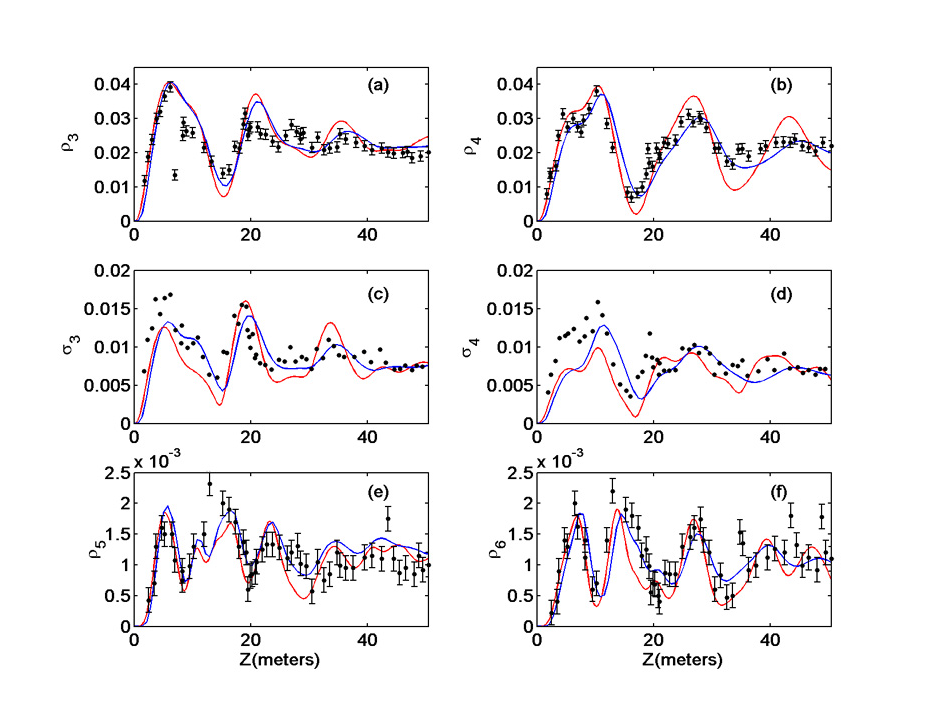
\includegraphics[width=6in]{nlsez55phaseornot.eps}
\end{center}
\renewcommand{\baselinestretch}{1}
\small\normalsize
\begin{quote}
\caption[Figure with caption indented]{This figure caption is indented and single-spaced.  Comparison between the experimental measurements \cite{hart1} (black), the random initial condition NLSE model excluding phase noise (dashed curves) and the stochastic phase noise NLSE model (solid curves) showing the first- and second-order sideband evolution as a function of fiber length for P$_{0} = 5.5$\,W, $\Omega = 366$\,GHz, $\Delta\nu = 0.5$\,GHz, $\gamma = 0.019$\,W$^{-1}$m$^{-1}$, and $\beta^{(2)} = 55$\,ps$^2$/km: dynamical evolution of the: (a) power in the first-order blue-shifted sideband, (b) power in the first-order red-shifted sideband, (c) fluctuations in the first-order blue-shifted sideband, (d) fluctuations in the first-order red-shifted sideband, (e) power in the second-order blue-shifted sideband, (f) power in the second-order red-shifted sideband. \label{fig:fig27}}
\end{quote}
\end{figure} 
\renewcommand{\baselinestretch}{2}
\small\normalsize

The first figure is Fig.\ref{fig:fig27}.   Please note that the figure label should be placed inside the figure caption.  
\newpage

The next figure is placed landscape.  It is Fig.~\ref{fig:mpc}.

\begin{landscape}
\renewcommand{\baselinestretch}{1}
\small\normalsize
\begin{quote}
\begin{figure}
\begin{center}
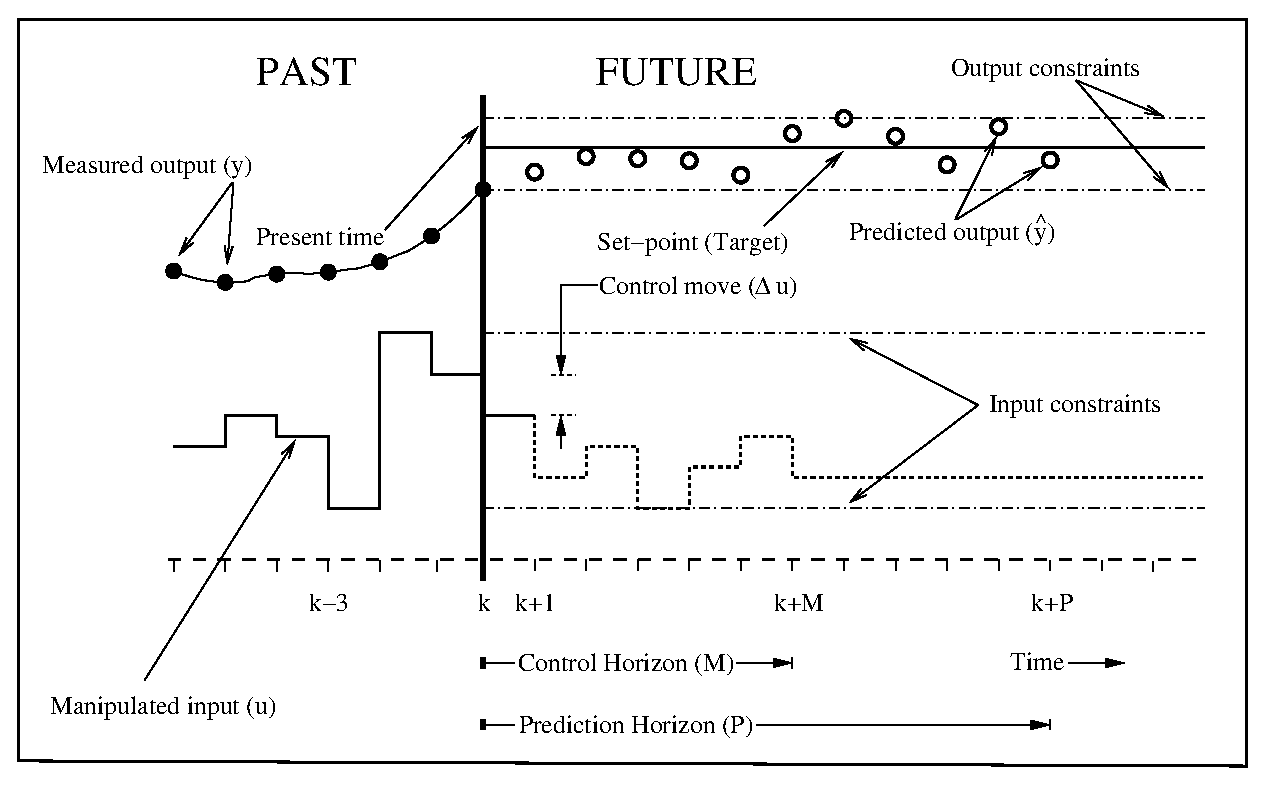
\includegraphics[width=8.2in]{mpc.eps}
\end{center}
\caption{Schematic illustrating receding horizon control.
\label{fig:mpc} }
\end{figure}
\end{quote}
\renewcommand{\baselinestretch}{2}
\small\normalsize
\end{landscape}

This is a my second figure which was placed landscape.  Although I have used the same figure, I have renamed the label to fig:mpc-1.  The second figure now becomes Figure~\ref{fig:mpc-1}.
\begin{landscape}
\renewcommand{\baselinestretch}{1}
\small\normalsize
\begin{quote}
\begin{figure}
\begin{center}
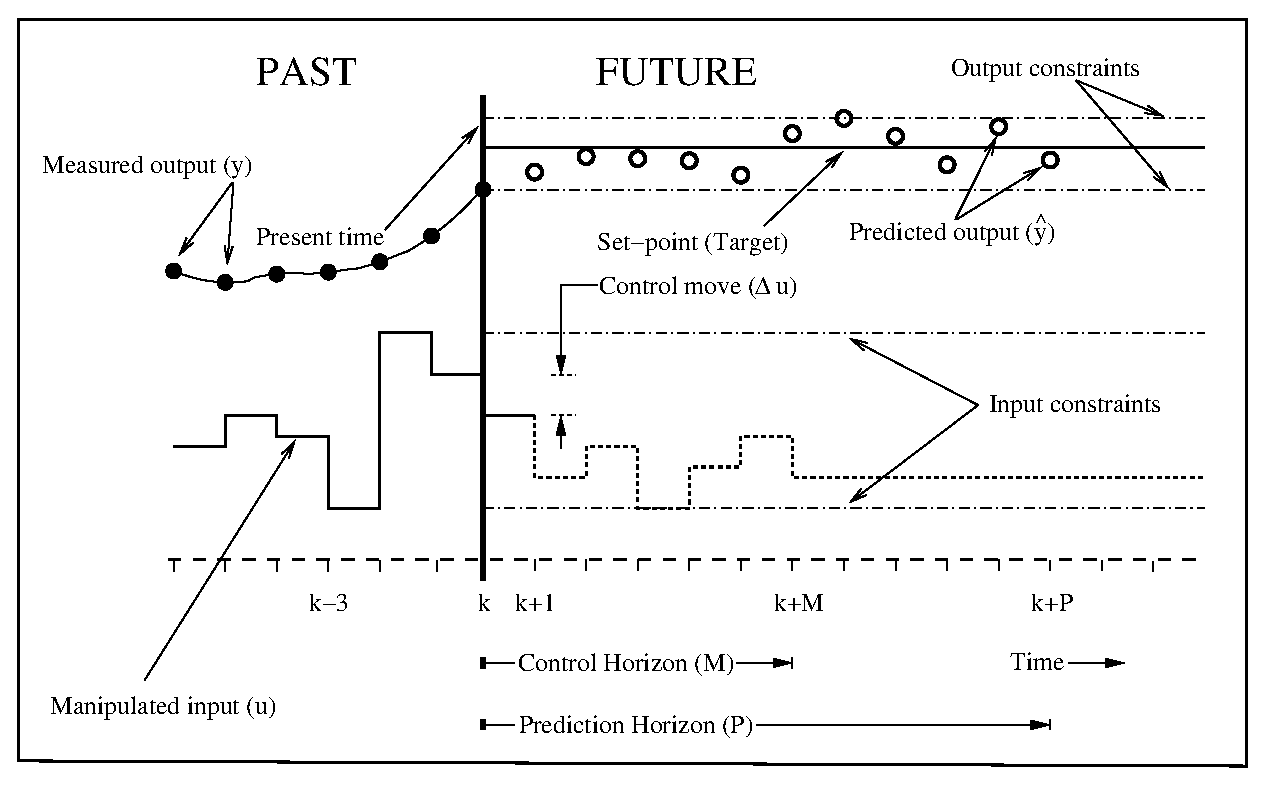
\includegraphics[width=8.2in]{mpc.eps}
\end{center}
\caption[Figure placed landscape on page]{Schematic illustrating receding horizon control. \label{fig:mpc-1}}
\end{figure}
\end{quote}
\renewcommand{\baselinestretch}{2}
\small\normalsize
\end{landscape}

\subsection{Numbering Figures}

If you wish your figures to be numbered 1-100 without any reference to the chapter (e.g., Figure 1.1, 2.1, etc.), change the first line of your mainthesis.tex file to read \begin{verbatim}"\documentclass[12pt]{thesis-2}".\end{verbatim}  

\subsubsection{This is a Subsubsection}

This is my first subsubsection in Chapter 1.


\section[Short Titles]{Short Titles in the Table of Contents, List of Figures, or List of Tables}

The Table of Contents, List of Figures, or List of Tables usually show the entire title of a section, subsection, etc. or table, or the entire caption of a figure.  If you put a short title in square brackets after \begin{verbatim} \section, \table, or \figure, \end{verbatim} the short title will show in your Table of Contents or lists.

\renewcommand{\baselinestretch}{1}
\small\normalsize

\begin{verbatim}
\section[Short Title]{Title of Section} 
\subsection[Short Title]{Title of Subsection} 
\end{verbatim}

or when using a caption in a figure or table
\begin{verbatim}
\caption[Short Caption]{Full text of the caption.}
\end{verbatim}

\renewcommand{\baselinestretch}{2}
\small\normalsize


\section{Figures on Text Page}

Normally figures in the thesis are placed on a page by themselves.  The following figure is placed on the page with text before and after the figure by adding [!!h] after \begin{verbatim} \begin{figure}[!!h] \end{verbatim}.  Please note that the figure label is placed within the caption.

\renewcommand{\baselinestretch}{1}
\large\normalsize

\begin{verbatim}
\begin{figure}[!!h]
 \begin{center}
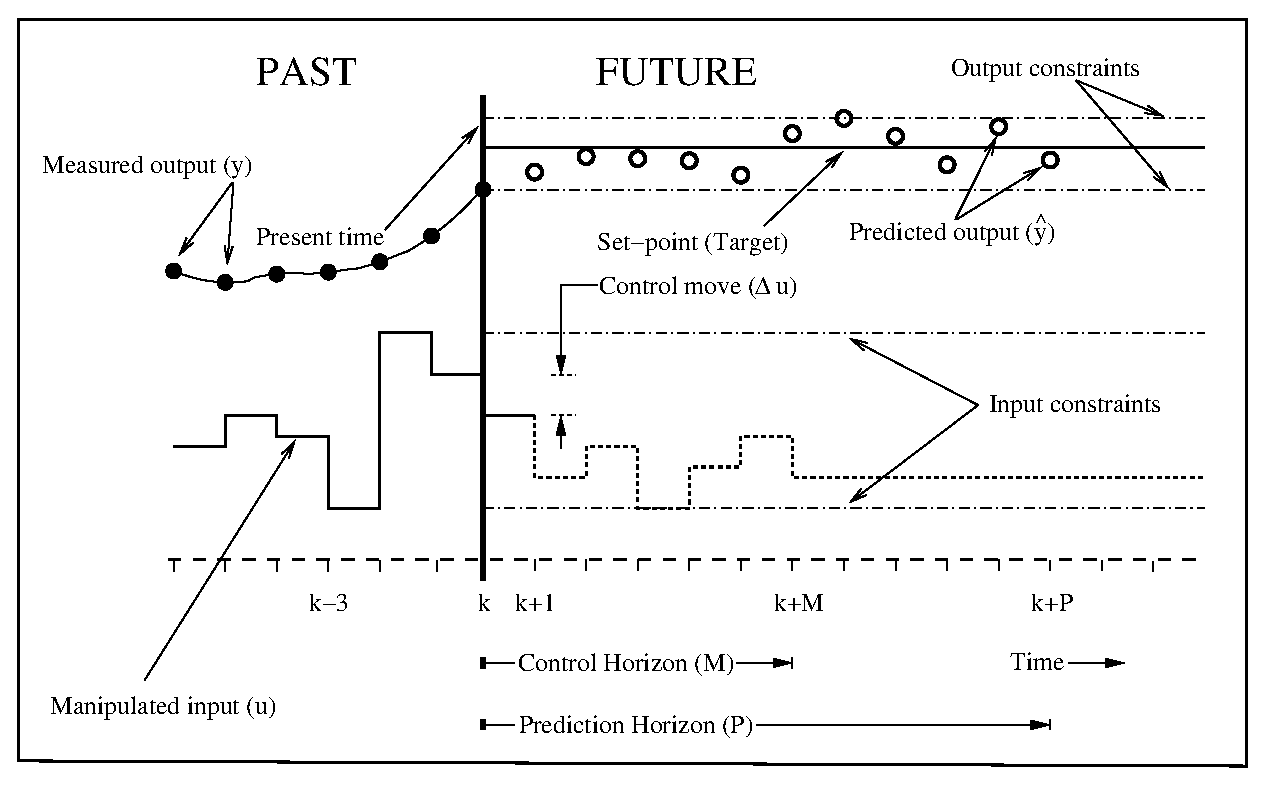
\includegraphics[width=5in]{mpc.eps}
\end{center}
\caption[Short title]{Schematic illustrating receding horizon control.
\label{fig:mpc-2}}
\end{figure}
\end{verbatim}

\begin{figure}[!!h]
 \begin{center}
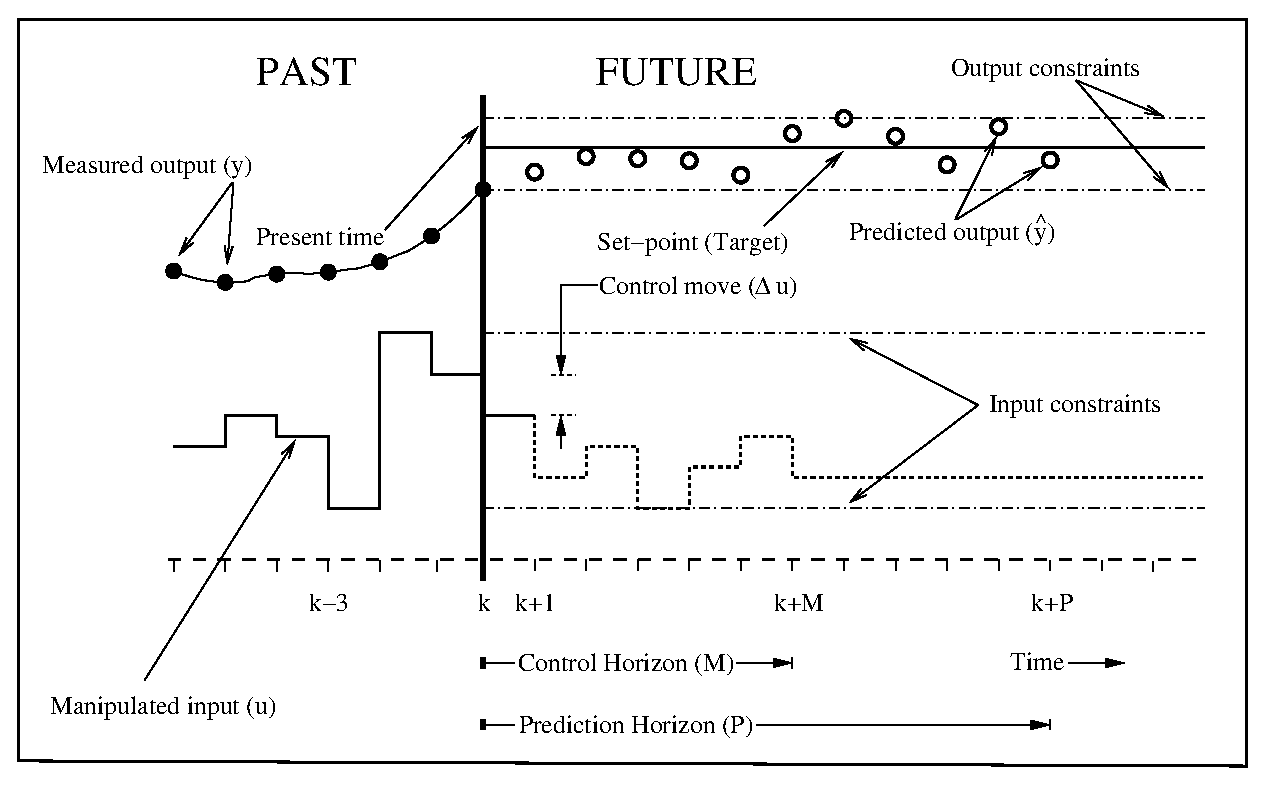
\includegraphics[width=5in]{mpc.eps}
\end{center}
\caption{Schematic illustrating receding horizon control. \label{fig:mpc-2}}
\end{figure}

\renewcommand{\baselinestretch}{2}
\large\normalsize

This does not necessarily mean that the text before and after the figure will be exactly what you want.  Remember Latex will place the figure where it will fit on the page the best.   The previous figure is Figs.~\ref{fig:mpc-2}. 

\section{Wrapping Text around Figure}


\renewcommand{\baselinestretch}{1}
\begin{wrapfigure}{r}{0.4\textwidth}
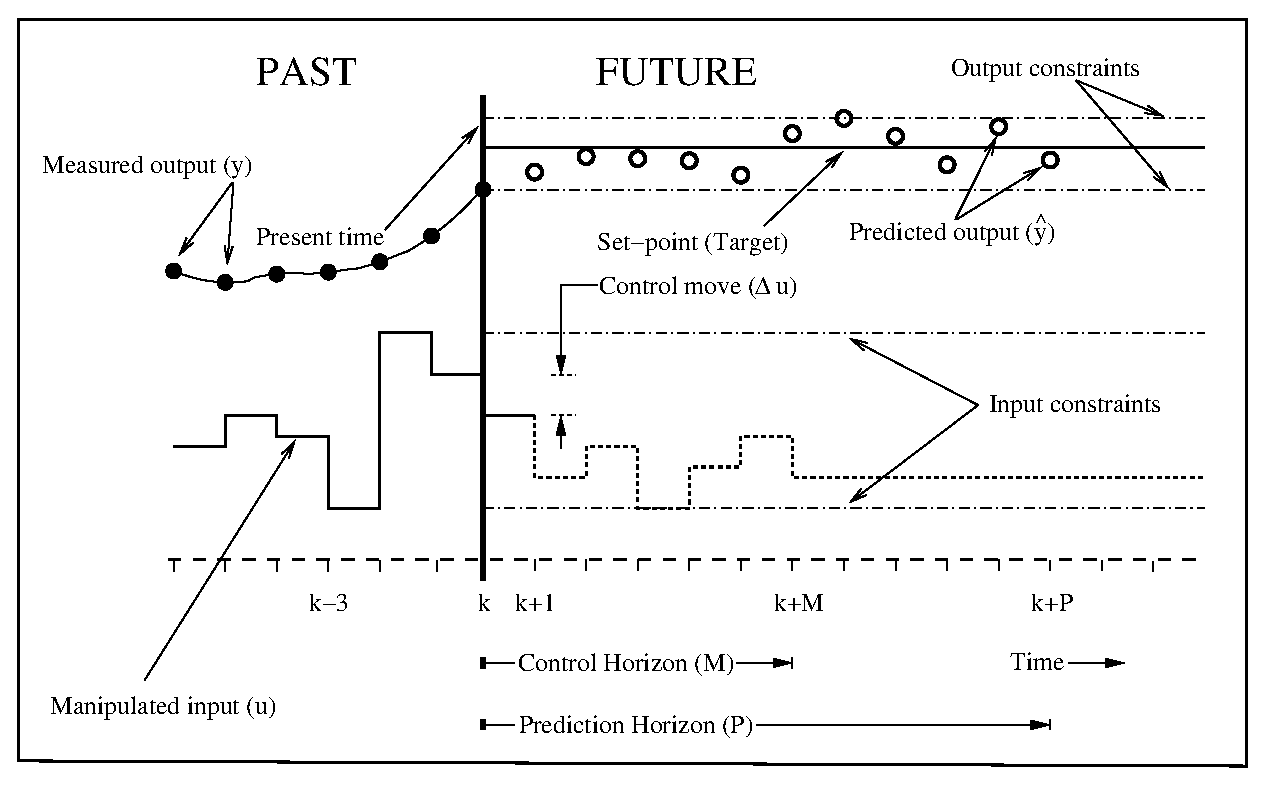
\includegraphics[width=0.4\textwidth]{mpc.eps}
\caption{ Text wrap around figure. \label{fig:test}}
\end{wrapfigure}

\renewcommand{\baselinestretch}{2}
\large\normalsize

By way of summary, at the end of the activity, I reminded the class of what we'd done:  by considering relatively nearby galaxies whose distance we had measured by some other means, we were able to establish a relationship locally between redshift and distance.  
By way of summary, at the end of the activity, I reminded the class of what we'd done:  by considering relatively nearby galaxies whose distance we had measured by some other means, we were able to establish a relationship locally between redshift and distance.  
By way of summary, at the end of the activity, I reminded the class of what we'd done:  by considering relatively nearby galaxies whose distance we had measured by some other means, we were able to establish a relationship locally between redshift and distance.  
By way of summary, at the end of the activity, I reminded the class of what we'd done:  by considering relatively nearby galaxies whose distance we had measured by some other means, we were able to establish a relationship locally between redshift and distance.  See Fig.~\ref{fig:test}.


\section{LaTeX -- A Typesetting Program}

A 13-page explanation of some of the features of LaTeX can be downloaded from http://www.jgsee.kmutt.ac.th/exell/General/LaTeX.html.


\section{Using Bibtex}

Using Bibtex with Latex documents is not difficult.  The bulk of the work is organizing your bibtex file, which is a data base compiled by you of the articles, books, etc. which you use in the bibliographies or reference sections of your publications.  

I have linked several files to this webpage, which will be helpful when you are using Bibtex.  These files can be downloaded from \newline
http://www.ireap.umd.edu/ireap/theses/bibtex.  Please read the file "BibtexInstructions.pdf".  The first two pages explain how to set up and run Bibtex; the remaining pages were taken from a published article and show how the references were cited in the .tex file.   The files BibtexInstructions.tex, Galactic.bib, Dottie.bib are the original .tex files used for BibtexInstructions.pdf.  The file BibtexSamples.tex contains examples of the information needed for the various publications you wish to reference (e.g., articles in refereed journals, books, unpublished articles, conference proceedings, etc.).

If you have questions concerning Bibtex, please contact me at 301-405-4955 or dbrosius at umd.edu.

\section{Using Natbib}

Another option of citing references in the bibliography is using Natbib instead of Bibtex.  You must still create a bibtex file, as noted above.  The command "backslash cite" cannot be used with natbib; instead "backslash citet" and "backslash citep" must be used.    "backslash citet" is used to show reference in the text (e.g., Eq.\ 8 in Reiser,1996 shows ...); "backslash citep" is used in the parenthetical (e.g., Eq.\ 8 (Reiser, 1996) shows ...).  

\begin{verbatim}
Add in preamble -- \usepackage[option]{natbib} 

Add at bottom of mainthesis.tex file --
\bibliography{name of your bibtex file}
\bibliographystyle{plainnat, abbrnat, or unsrtnat}
\end{verbatim}

Typesetting:   Latex, Bibtex, Latex, Latex

The reference sheet for natbib usage can be found at \newline "http://merkel.zoneo.net/Latex/natbib.php".

\section{APS Physical Review Style and Notation Guide}

The following style guide may be downloaded from The American Physical Society at http://forms.aps.org/author/styleguide.pdf:  Physical Review Style and Notation Guide, published by The American Physical Society, compiled and edited by Anne Waldron, Peggy Judd, and Valerie Miller, February 1993.  It may be old, but it is very useful.

			%Chapter 1

\renewcommand{\thechapter}{1}

\chapter{Ultracold Atomic Systems}

\section{Degenerate quantum gases}

Degenerate quantum gases rock. Many years have passed since a handful of really smart people realized that the macroscopic properties comprising the thermodynamic state of a system can emerge from the right statistical ensembles of single particle behaviour or misbehaviour. For most models the math is relatively simple and the physics are intuitive, so in part thanks to the wonders of quantum degeneracy, things are kept rather simple in this thesis. 

A definition for quantum degeneracy is that the motional state of an ensemble of particles in equilibrium becomes maximally degenerate. Bosons, who are famous for liking each other, bunch in some state while fermions, in a more discriminaory fashion, occupy states according to the Pauli exclusion principle.

Quantum degeneracy has been experimentally realized for a couple of systems, most notably for dilute clouds of very cold atoms, where energy can take various forms ranging a couple of different energy scales. For instance if we pick an alkali atom (first column of your favorite periodic table), the known atomic structure has energy splittings of no more than a couple $\rm{eV}$ which is roughly $1/10 ^{22}$ of the energy input needed to fill the battery of a smartphone. If this was not ridiculous enough, the temperatures at which these gases finally become degenerate are close to $100 \, \rm{nK}$ which is roughly a trillionth of that. The diluteness of these gases only adds to their finesse, as typical densities range a few tens of trillions of particles per cubic centimeter, which compared to the air we breathe is about a hundred thousand times less dense. 

The aspect of these sysems can be really diverse, but it useful for now to imagine a $10\, \rm{\mu m}$ blob, close to the actual size of a white-blood cell (or a tenth of the width of a human hair), floating around an ultra high vacuum (UHV) environment isolated from everything while being held by an optical trap. How one goes about making one of these is the subject of the next section.


\section{Making a quantum degenerate gas}

Mathematically speaking, in the classical limit, pulse propagation in an
optical fiber is governed by Maxwell's equations \cite{Agrawal2,Diament}, 
%1.5
\begin{eqnarray} 
\vec{\nabla}\times\vec{E} & = &- {\partial \vec{B} \over \partial t} \nonumber\\
\vec{\nabla}\times\vec{H} & = & \vec{J}+ {\partial \vec{D} \over \partial t}
\nonumber\\ 
\vec{\nabla}\cdot\vec{D} & = & \rho_{f} \nonumber\\
\vec{\nabla}\cdot\vec{B} & = & 0 ,
\end{eqnarray}
where $\vec{E}$ and $\vec{H}$ are electric and magnetic field
vectors, and
$\vec{D}$ and $\vec{B}$ are electric and magnetic flux densities, 
respectively. $\vec{J}$ is the current density and $\rho_{f}$ is the free
charge density.

This is the second equation array.
\begin{eqnarray}
W & = & \int d^3{\rm r} \left[ \sum_s \left( \int d^3{\rm v} \right){T_{s} \langle h^2_s \rangle {\rm r} \over 2F_{0s}} \right] + {|\delta \rm B|^2 \over 8\pi} \nonumber \\ 
& = & \int d^3 
\end{eqnarray}

Under the following assumptions \cite{Agrawal2} -
\begin{enumerate}
\item[(a)]
there are no free charges ($\vec{J}=\rho_{f}=0$), a good approximation for an optical fiber, 
\item[(b)] the medium is non-magnetic ($\vec{M}=0$), which an optical fiber is,
\item[(c)] the wavelength of light propagated is away from any material
resonances (0.5 - 2 $\mu$m), the results described in this thesis lie in this wavelength range, i.e., the results presented in Chap.\ 2 and Chap.\ 3 lie in the 600-700\,nm regime and the results presented in Chap.\ 4 lie in the 800\,nm regime,
\item[(d)] the electric-dipole approximation is valid, due to which the second-order parametric processes such as three-wave-mixing and second harmonic generation can be neglected (in practice they do occur because of quadrupole and magnetic-dipole effects but with a very low efficiency),
\item[(e)] the medium only responds locally, which is a valid approximation for the projects considered herein,
\item[(f)] the nonlinear polarization $\vec{P}_{NL}$ can be taken as a
perturbation to the total induced polarization $\vec{P}$, which is justified as the nonlinear effects are relatively weak for the results presented in this thesis,
\item[(g)] only 3rd order nonlinear effects need to be taken into
account, which is valid up to 5th order in ${\bf E}$ since the 2nd and 4th order effects are absent due to the centrosymmetric nature of the disordered liquidlike state of fused silica,
\item[(h)] the imaginary part of the dielectric constant
$\epsilon(\omega)$ is small compared to the real part (low loss, which is a good approximation for the wavelength regimes and fiber lengths considered here),
\item[(i)] the wavelength of light is higher than the cutoff wavelength
of the fiber so that the single transverse mode condition is satisfied (or else there would be multimode propagation and nonuniform modal dispersion would have to be taken into account),
\item[(j)] the optical fiber is polarization maintaining and the light
pulse is traveling along one of the 2 principal axes of the fiber, a very good approximation for the results of Chap.\ 2, and Chap.\ 3, in the case of Chap.\ 4, this approximation is relaxed as the incident light travels along both axes of the fiber, thus requiring a set of two coupled NLSEs for simulation, one for each axis,
\item[(k)] the slowly varying envelope approximation is valid, i.e.,
$\Delta\omega/\omega_{0} \ll 1$ where $\Delta \omega$ is the spectral
width of the pulse spectrum which is centered at $\omega_{0}$, this approximation is valid for the studies considered in Chap.\ 2 and Chap.\ 4, in Chap.\ 3, the Raman Stokes wave is considered as a separate slowly varying envelope from the pump wave, as the two taken together would not satisfy this condition,
\item[(l)] the nonlinear response of the medium is instantaneous, an
approximation valid for pulse widths greater than $\sim$70\,fs, which amounts to neglecting the contribution of molecular vibrations to $\chi^{(3)}$ (the Raman effect), which have been included in the study presented in Chap.\ 4 since the pulse width was $\sim$ 140\,fs.
\end{enumerate}
The propagation of the slowly varying envelope A(z,t) of a light
pulse
along an optical fiber is governed by the nonlinear partial
differential equation \cite{Agrawal2} -
%1.6
\begin{equation}
{\partial A \over \partial z} + \beta_{1} {\partial A \over \partial t} + {i \beta_{2} \over 2} {\partial^{2} A \over \partial t^{2}} = i \gamma |A|^{2}A,
\end{equation}
where $v_{g}=1/\beta_{1}$ is the group velocity of the pulse,
$\beta_{2}$
is the group velocity dispersion coefficient, %$\alpha$ is the fiber loss,
and $\gamma$ is the nonlinearity coefficient given by
%1.7
\begin{equation}
\gamma = {n_{2}\omega_{0} \over c A_{eff}} .
\end{equation}

Here $\omega_{0}$ is the central angular frequency of the pulse and
A$_{eff}$, the effective core area of the fiber.

Under transformation to  a frame of reference moving at the group
velocity of the pulse, the above equation takes the form of the so-called
`nonlinear Schr\"odinger equation' (NLSE), i.e.,
%1.8
\begin{equation}
{\partial A \over \partial z} + {i\beta_2 \over 2} {\partial^2
A \over \partial \tau^2} = i \gamma |A|^2A ,
\end{equation}
where
%1.9
\begin{equation}
\tau = t - {z \over v_g}
\end{equation}
is time measured in a frame of reference moving at the group
velocity
v$_g$ of the pulse.

\section{Numerical Pulse Propagation}

The NLSE, like most nonlinear partial differential equations, is not
amenable to analytical solution except in certain special cases where the
inverse scattering transform can be used \cite{Zakharov}. Thus a
numerical approach is necessary for understanding the physics of phenomena
governed by the NLSE. The numerical methods available can be classified as
finite-difference techniques and pseudo-spectral techniques. Usually
pseudo-spectral methods are an order of magnitude faster, the most
popular method being the Split-Step Fourier Method (SSFM) \cite{Agrawal2,Hardin,
Fisher}. The speed of the SSFM can be partly attributed to the use
of the finite fast-Fourier transform (FFT) algorithm
\cite{Cooley}.For an algorithmic description of the SSFM the reader is
referred to Chap.\ 2, Sec.\ 2. Therein is also described an
unconditionally stable scheme for including linear multiplicative noise into
the SSFM without disturbing the conservative properties of the NLSE. In the
projects described in Chap.\ 3, simulations were carried out using a
combination of the SSFM and finite difference schemes. The SSFM is also used 
 to arrive at the simulated results described in Chap.\ 4.

\section{Experimental Pulse Diagnostics}

With the advent of frequency resolved optical gating
(FROG) \cite{Trebino,Kanejqe,Kaneoptlett}, it has become possible to not
only measure the optical spectrum and optical time trace of a light pulse
but to measure the full electric field envelope (intensity and phase) of the
light pulse. The two fields of nonlinear fiber optics and frequency resolved
optical gating (FROG) are yet to undergo cross pollination to their fullest
potential since the inception of FROG 10 years ago. This novel experimental
technique adds new dimensions to pulse measurement techniques, one of which
is the ability to measure how asymmetric a pulse is, i.e., measure its
skewness, kurtosis and all higher order moments. Asymmetric pulse
propagation is a subject of interest in Chap.\ 4, where a highly simplified
version of FROG \cite{OShealett} is used to measure pulse characteristics
before and after a fiber.

\section{Group Velocity Dispersion}

Group velocity dispersion \cite{Agrawal3} (GVD) involves the temporal broadening of a pulse as it propagates through an optical fiber. From the NLSE (Eq.\ 1.6) one can derive length scales relevant to linear dispersion (L$_{D}$=T$_{0}^{2}$/$\beta_{2}$) and nonlinearity (L$_{NL}$=1/$\gamma$P$_{0}$). Here T$_{0}$ is the pulse width and P$_{0}$ is the peak power of the pulse. The regime in which the effects of GVD dominate and the effects of nonlinearity are negligible is given by -
%1.10
\begin{equation}
{L_{D} \over L_{NL}}={\gamma P_{0} T_{0}^{2} \over |\beta_{2}|} \ll 1 .
\end{equation}

In this regime, optical pulses propagate as they undergo symmetric temporal broadening and linear chirping without any spectral broadening. The sign of the GVD parameter $\beta_{2}$ determines the sign of the induced chirp. If the input pulse is chirped, then it may undergo some initial pulse compression followed by temporal broadening. Unlike the second-order dispersion associated with GVD, third-order dispersion causes asymmetric temporal broadening with leading and trailing edges. It becomes important, when the operating wavelength is near the zero dispersion wavelength of the fiber (the wavelength at which $\beta_{2}$=0). GVD starts to limit optical fiber communication systems when consecutive pulses broaden so much that they start to overlap.   

\section{Self-Phase Modulation}

Self-phase modulation \cite{Agrawal4} (SPM) is a phenomenon that leads to spectral broadening and modulation of optical pulses. In the absence of GVD, SPM induced spectral broadening occurs without change in the temporal pulse shape. The spectral broadening occurs as a consequence of an intensity dependent phase-shift. The project described in Chap.\ 2 has the property that L$_{NL}$ $<$ L $\ll$ L$_D$, i.e., the nonlinear term representing SPM dominates. In the regime where both SPM and GVD are non-negligible (as in Chap.\ 4), phenomena qualitatively different from those described in this section and the previous section can occur. Both temporal and spectral broadening can occur simultaneously. In the regime of femtosecond pulse propagation (as in Chap.\ 4), GVD, third-order dispersion, intrapulse Raman scattering (discussed in Chap.\ 2) and higher order nonlinear effects have to be taken into account. If the input pulse is asymmetric, then SPM effects dominate over all other effects, as is observed in Chap.\ 3. In some cases SPM can lead to pulse compression, and in the anomalous dispersion regime ($\beta_2 < 0$), the balance between GVD and SPM can lead to soliton formation. 

\section{Four-wave-mixing}

Four-wave-mixing (FWM) \cite{Agrawal10} is a parametric process involving
the interaction
between four photons at different frequencies. Two different kinds of
four-wave-mixing processes are possible -
%1.11
\begin{eqnarray}
\omega_4 = \omega_1 + \omega_2 + \omega_3 \\
\omega_3 + \omega_4 = \omega_1 + \omega_2 .
\end{eqnarray}

The former process results in third harmonic generation for the special case
when $\omega_1 = \omega_2 = \omega_3$. Both processes require phase
matching to occur, in order to be efficient. For the latter case, with
the partial degeneracy of $\omega_1 = \omega_2$, it is relatively easy
to satisfy the phase matching condition of
%1.12
\begin{equation}
\Delta k = k_3 + k_4 - k_1 - k_2 = 0 .
\end{equation}

This process is of great interest to nonlinear dynamicists as the
evolution of the FWM process could constitute a route to chaos further
down-stream in the fiber. It is also of great interest to people working in
the field of optical communication systems, as it can cause cross-talk
between neighboring channels in a wavelength division multiplexing scheme
of communication.

\section{Cross-Phase Modulation}

Cross-phase modulation (XPM) \cite{Agrawal7} occurs in optical fibers when
two or more optical pulses having different central wavelengths propagate 
simultaneously inside a fiber, interacting through the fiber
nonlinearity which couples the two pulses nonlinearly.  The evolution of the
two pulses depends on the group velocity mismatch between them by virtue of 
their being centered at different wavelengths, although this is a linear
phenomenon. The group velocity mismatch also exists between light pulses
traveling along orthogonal polarization axes of a fiber, and centered around
identical wavelengths, since the slow axis and fast axis of the fiber have
different group velocities. In this case, too, the two polarizations interact
nonlinearly \cite{Agrawal6} through degenerate XPM (degenerate since the
central wavelengths are the same). In the case of degenerate XPM the 2nd order 
and higher dispersion parameters, and the nonlinear parameters (all of which
depend only on the wavelength), are also the same unlike in general XPM. The 
effects of XPM are more pronounced when one of the pulses (the pump) has much 
higher power than the other (the probe). Otherwise, the effects of self-phase 
modulation (SPM) tend to dominate.

\section{Stimulated Inelastic Scattering} 

Other nonlinear effects (apart from those due to the cubic $\chi^{(3)}$
nonlinearity) arise due to the interaction between the light
traveling in the fiber and the fiber medium. Interactions between
the light field and the vibrational levels of the fiber medium lead to
stimulated Brillouin scattering (SBS) and stimulated Raman
scattering (SRS). SRS and SBS were among the first nonlinear effects
studied in optical fibers \cite{Stolen,Ippen,Smith}.  In a simple quantum
mechanical picture \cite{Agrawal1} applicable to
both SRS and SBS, a photon of the incident field (called the pump) is
annihilated to create a photon at a lower frequency (belonging to the
Stoke's wave) and a phonon to conserve energy and momentum. SBS involves
an acoustic phonon whereas SRS involves an optical phonon, thus they have
qualitatively different dispersion relations. SBS has a much
lower threshold power and manifest itself through a backward propagating
wave in contrast to SRS which can involve both forward and backward
traveling waves. SBS has a maximum gain at a frequency 10\,GHz \cite{Agrawal9}
(down-shifted with respect to the pump) and
requires a very narrow bandwidth pump to manifest itself. SRS, in
contrast, has a maximum gain at a frequency 13\,THz \cite{Agrawal8} downshifted with
respect to the pump. For pulse-bandwidths larger than 13\,THz, the
phenomenon of Intrapulse Raman Scattering (IRS) manifests itself,
involving a self-frequency shift within the pulse from higher frequency
components to lower frequency components. Thus, SRS
becomes more important for shorter pulses (larger bandwidth) unlike SBS
which nearly ceases to occur for pulses shorter than 10\,ns. In both SRS
and SBS, the optical fiber plays an active role in the nonlinear process,
unlike the case of cross- and self-phase modulation, four-wave-mixing and
third harmonic generation, where the fiber plays a passive role by
mediating the interaction between several optical waves.

\section{Outline of Thesis}

In Chap.\ 2, we present the results of a computational study of the
influence of stochasticity on the dynamical evolution of multiple 
four-wave-mixing processes in a single mode optical fiber with spatially
and temporally $\delta$-correlated phase noise. A generalized nonlinear
Schr\"odinger equation (NLSE) with stochastic phase fluctuations along the
length of the fiber is solved using the Split-step Fourier method
(SSFM). Good agreement is obtained with previous experimental and
computational results based on a truncated-ODE (Ordinary Differential
Equation) model in which stochasticity was seen to play a key role in
determining the nature of the dynamics. The full NLSE allows for
simulations with high frequency resolution (60\,MHz) and frequency span (16
THz) compared to the truncated ODE model (300\,GHz and 2.8\,THz,
respectively), thus enabling a more detailed comparison with
observations. A physical basis for this hitherto phenomenological phase
noise is discussed and quantified.

In Chap.\ 3, we discuss the implications of spontaneous and stimulated
Raman scattering on the project discussed in Chap.\ 2, namely, the dynamical evolution of 
stochastic four-wave-mixing processes in an optical fiber.
The following question is asked - can stimulated Raman scattering be a mechanism by which
adequate multiplicative stochastic phase fluctuations are introduced in the 
electric field of light undergoing four-wave-mixing as? Adequately checked numerical
algorithms of stimulated Raman scattering (SRS), spontaneous Raman generation and intrapulse 
Raman scattering (IRS) are used while exploring this issue. The algorithms are described in detail, as also are 
the results of the simulations. It is found that a 50-meter length of fiber (as used in the experiments),
is too short to see the influence of Raman scattering, which is found to eventually 
dominate for longer fiber lengths.

In Chap.\ 4, self- and cross-phase modulation (XPM) of femtosecond pulses ($\sim$ 810
nm) propagating through a birefringent single-mode optical fiber ($\sim$ 6.9
cm) is studied both experimentally (using GRENOUILLE - Grating Eliminated 
No Nonsense Observation of Ultrafast Laser Light Electric Fields) 
%(using second harmonic
%generation-frequency resolved optical gating or SHG-FROG) 
and numerically
(by solving a set of coupled nonlinear Schr\"odinger equations or
CNLSEs). An optical spectrogram representation is derived from the
electric field of the pulses and is linearly juxtaposed with the
corresponding optical spectrum and optical time-trace. The effects of
intrapulse Raman scattering (IRS) are discussed and the question whether 
it can be a cause of asymmetric tranfer of pulse energies towards longer 
wavelengths is explored. The simulations are shown to be in good qualitative 
agreement with the experiments. Measured input pulse asymmetry, when incorporated 
into the simulations, is found to be the dominant cause of output spectral 
asymmetry. \renewcommand{\baselinestretch}{1} \small\footnotesize
\footnote{These averages are reported
for $45$ `detailed occupational codes', which is an intermediate
occupational classification (between two and three-digit codes)
given by the Current Population Survey (CPS).}
\renewcommand{\baselinestretch}{2} \small\normalsize
The results indicate that it is possible to modulate short pulses both temporally and spectrally by passage through polarization maintaining 
optical fibers with specified orientation and length. The modulation technique is very direct and straightforward. No frequency components of the broadband pulse have to be rejected as the entire spectrum is uniformly modulated. The technique is flexible as the modulation spacing can be varied by varying the fiber length.

Chapter 5 provides the conclusion to the thesis.

\section{Theorems}

\newtheorem{theorem}{Theorem}[chapter]
\begin{theorem}
This is my first theorem.
\end{theorem}


\section{Axioms}
\newtheorem{axiom}{Axiom}[chapter]
\begin{axiom}
This is my first axiom.
\end{axiom}

\begin{axiom}
This is my second axiom in chapter 1.
\end{axiom}

\section{Tables}

This is my table. 

\renewcommand{\baselinestretch}{1}
\small\normalsize

\begin{table}[h]
\caption[Short title]{Overview of test cases used in this study.}
\begin{center}
\begin{tabular}{|c|c|c|c|}
\hline
Test & Quality & Setpoint & Manipulated \\
case & variable (QV) & for QV & variables (MVs)\\
\hline \hline
TE & G/H ratio & 1.226 & D-feed SP and Reactor Level SP\\
AZ & xB($H_2O$) & & Reflux flow and $5^{th}$ Tray temperature SP\\  
\hline
\end{tabular}
\end{center}
\label{test_over}
\end{table}

\renewcommand{\baselinestretch}{2}
\small\normalsize

My table is shown above.   Normally it is double-spaced but I have inserted a command (marked in blue) to make it single-spaced and then inserted a command (again in blue) to change the text back to double-spacing.

\

\subsection{Adding Extra Space between Text and Horizontal Lines}

\renewcommand{\baselinestretch}{1}
\small\normalsize

\setlength{\tablinesep}{5ex}

\begin{table}[h]
\caption{Table with Extra Space between the Text and Horizontal Lines.}
\begin{center}
\begin{tabular}{|p{.5in}|p{1in}|c|p{2.25in}|}
\hline
Test case& Quality variable QV)& Setpoint for QV & Manipulated  variables (MVs)\\
\hline \hline
TE & G/H ratio & 1.226 & D-feed SP and Reactor Level SP\\ \hline
AZ & xB($H_2O$) & & Reflux flow and $5^{th}$ Tray temperature SP \\
\hline
\end{tabular}
\end{center}
\label{test_over}
\end{table}

\renewcommand{\baselinestretch}{2}
\small\normalsize

The line \begin{verbatim}\usepackage{tabls}\end{verbatim} must be inserted in the preamble of your document.
The table is set up to be single-spaced by \begin{verbatim} \renewcommand{\baselinestretch}{1} \small\normalsize\end{verbatim} before \begin{verbatim}\begin{table}\end{verbatim}.  I set the first, second, and fourth columns as paragraphs, .5in, 1in, and 2.25in wide, respectively.  I then adjusted the separation between the words and the horizontal lines to 5ex by also adding \begin{verbatim}\setlength{\tablinesep}{5ex}\end{verbatim} before the \begin{verbatim}\begin{table}\end{verbatim} command.

After typing the table I change the document to be double-spaced from this point on.

\newpage


\section{Figures}

The figure on the following page is centered and the figure caption is indented and single-spaced.  Make sure you copy the last two lines \begin{verbatim}
\renewcommand{\baselinestretch}{2}\\
\small\normalsize\end{verbatim} to return to double-spacing of your text.

\begin{figure}
\begin{center}
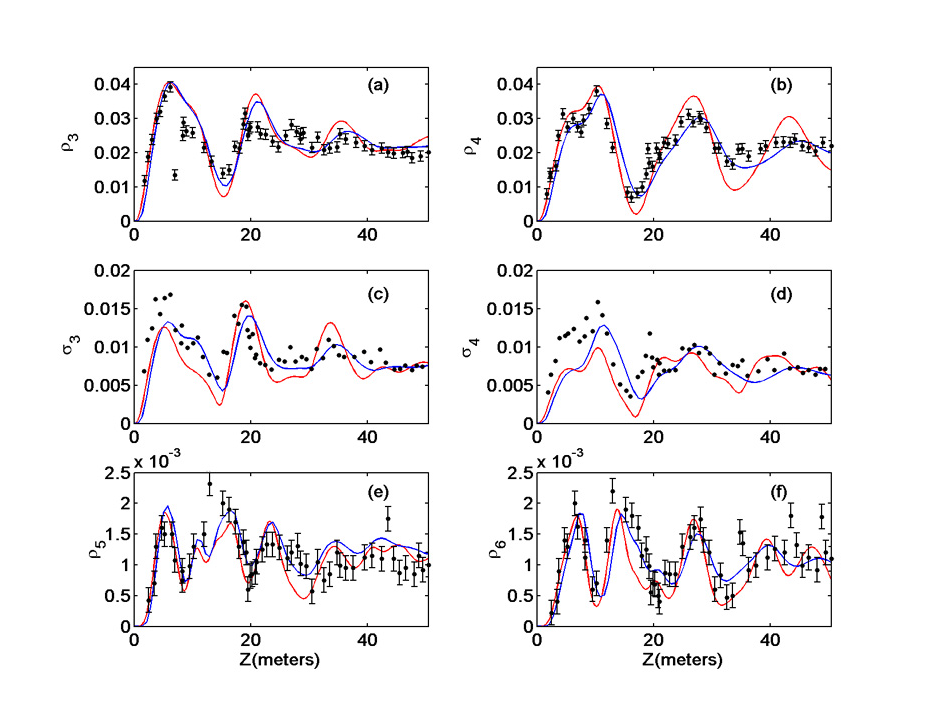
\includegraphics[width=6in]{nlsez55phaseornot.eps}
\end{center}
\renewcommand{\baselinestretch}{1}
\small\normalsize
\begin{quote}
\caption[Figure with caption indented]{This figure caption is indented and single-spaced.  Comparison between the experimental measurements \cite{hart1} (black), the random initial condition NLSE model excluding phase noise (dashed curves) and the stochastic phase noise NLSE model (solid curves) showing the first- and second-order sideband evolution as a function of fiber length for P$_{0} = 5.5$\,W, $\Omega = 366$\,GHz, $\Delta\nu = 0.5$\,GHz, $\gamma = 0.019$\,W$^{-1}$m$^{-1}$, and $\beta^{(2)} = 55$\,ps$^2$/km: dynamical evolution of the: (a) power in the first-order blue-shifted sideband, (b) power in the first-order red-shifted sideband, (c) fluctuations in the first-order blue-shifted sideband, (d) fluctuations in the first-order red-shifted sideband, (e) power in the second-order blue-shifted sideband, (f) power in the second-order red-shifted sideband. \label{fig:fig27}}
\end{quote}
\end{figure} 
\renewcommand{\baselinestretch}{2}
\small\normalsize

The first figure is Fig.\ref{fig:fig27}.   Please note that the figure label should be placed inside the figure caption.  
\newpage

The next figure is placed landscape.  It is Fig.~\ref{fig:mpc}.

\begin{landscape}
\renewcommand{\baselinestretch}{1}
\small\normalsize
\begin{quote}
\begin{figure}
\begin{center}
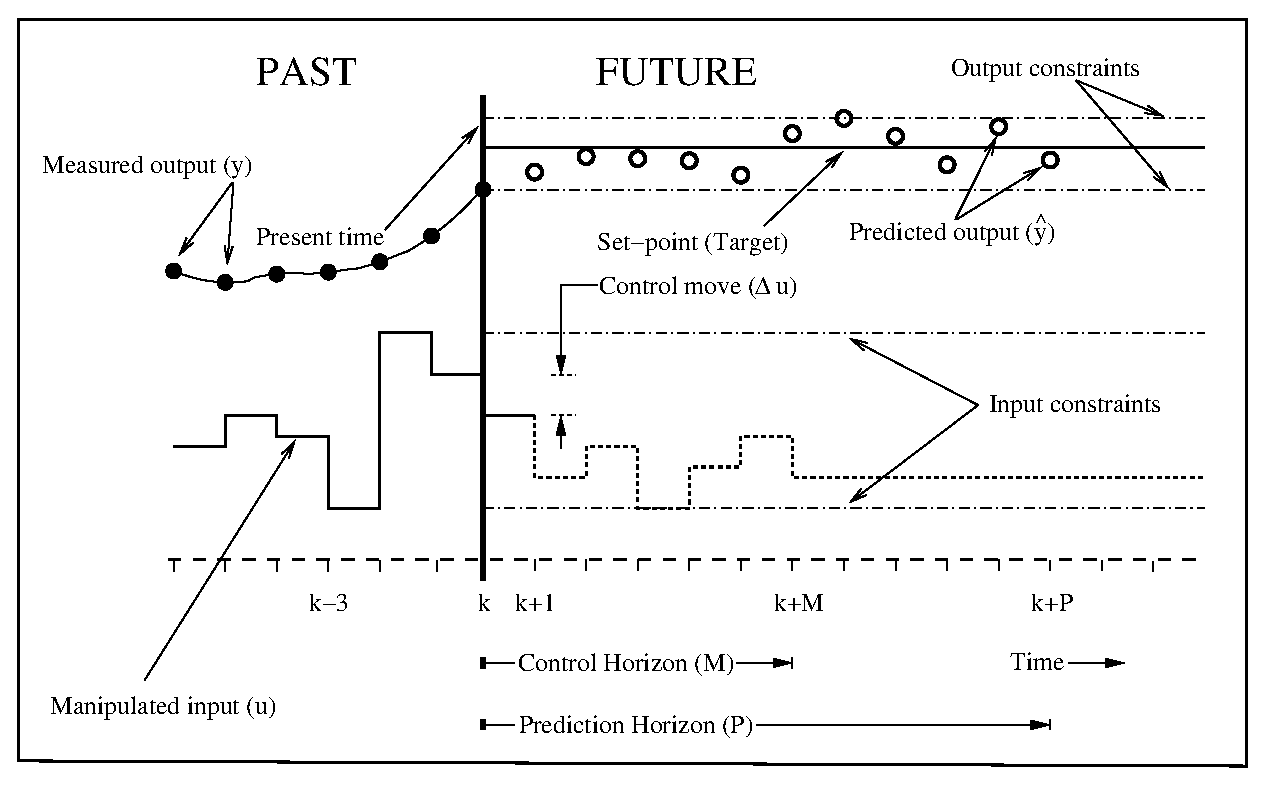
\includegraphics[width=8.2in]{mpc.eps}
\end{center}
\caption{Schematic illustrating receding horizon control.
\label{fig:mpc} }
\end{figure}
\end{quote}
\renewcommand{\baselinestretch}{2}
\small\normalsize
\end{landscape}

This is a my second figure which was placed landscape.  Although I have used the same figure, I have renamed the label to fig:mpc-1.  The second figure now becomes Figure~\ref{fig:mpc-1}.
\begin{landscape}
\renewcommand{\baselinestretch}{1}
\small\normalsize
\begin{quote}
\begin{figure}
\begin{center}
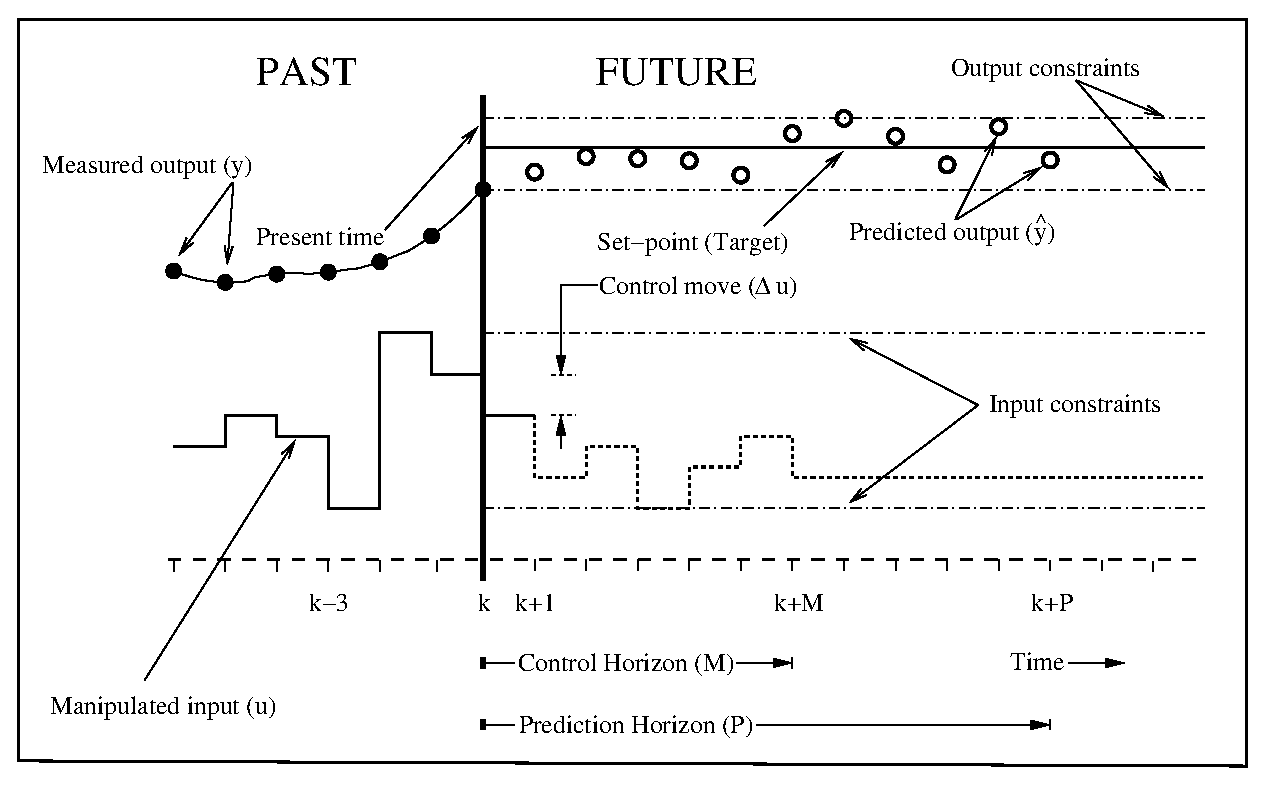
\includegraphics[width=8.2in]{mpc.eps}
\end{center}
\caption[Figure placed landscape on page]{Schematic illustrating receding horizon control. \label{fig:mpc-1}}
\end{figure}
\end{quote}
\renewcommand{\baselinestretch}{2}
\small\normalsize
\end{landscape}

\subsection{Numbering Figures}

If you wish your figures to be numbered 1-100 without any reference to the chapter (e.g., Figure 1.1, 2.1, etc.), change the first line of your mainthesis.tex file to read \begin{verbatim}"\documentclass[12pt]{thesis-2}".\end{verbatim}  

\subsubsection{This is a Subsubsection}

This is my first subsubsection in Chapter 1.


\section[Short Titles]{Short Titles in the Table of Contents, List of Figures, or List of Tables}

The Table of Contents, List of Figures, or List of Tables usually show the entire title of a section, subsection, etc. or table, or the entire caption of a figure.  If you put a short title in square brackets after \begin{verbatim} \section, \table, or \figure, \end{verbatim} the short title will show in your Table of Contents or lists.

\renewcommand{\baselinestretch}{1}
\small\normalsize

\begin{verbatim}
\section[Short Title]{Title of Section} 
\subsection[Short Title]{Title of Subsection} 
\end{verbatim}

or when using a caption in a figure or table
\begin{verbatim}
\caption[Short Caption]{Full text of the caption.}
\end{verbatim}

\renewcommand{\baselinestretch}{2}
\small\normalsize


\section{Figures on Text Page}

Normally figures in the thesis are placed on a page by themselves.  The following figure is placed on the page with text before and after the figure by adding [!!h] after \begin{verbatim} \begin{figure}[!!h] \end{verbatim}.  Please note that the figure label is placed within the caption.

\renewcommand{\baselinestretch}{1}
\large\normalsize

\begin{verbatim}
\begin{figure}[!!h]
 \begin{center}
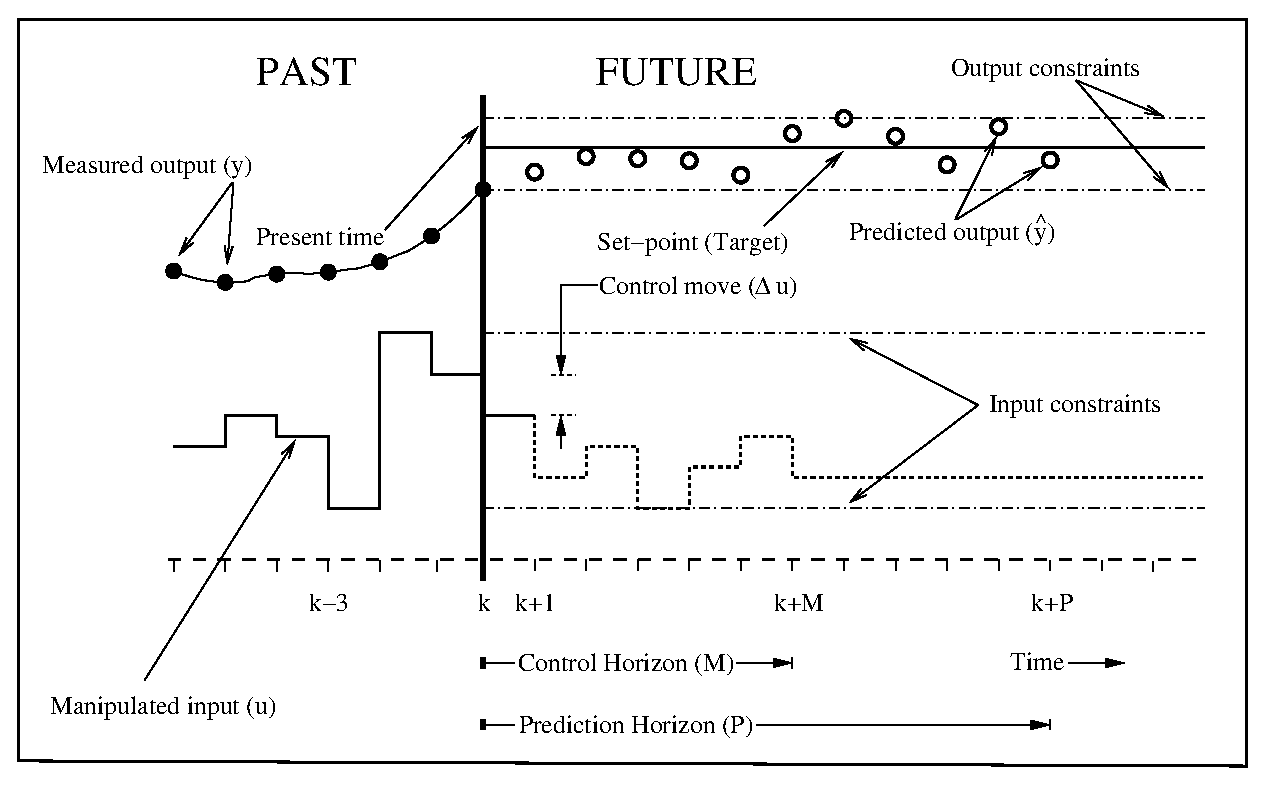
\includegraphics[width=5in]{mpc.eps}
\end{center}
\caption[Short title]{Schematic illustrating receding horizon control.
\label{fig:mpc-2}}
\end{figure}
\end{verbatim}

\begin{figure}[!!h]
 \begin{center}
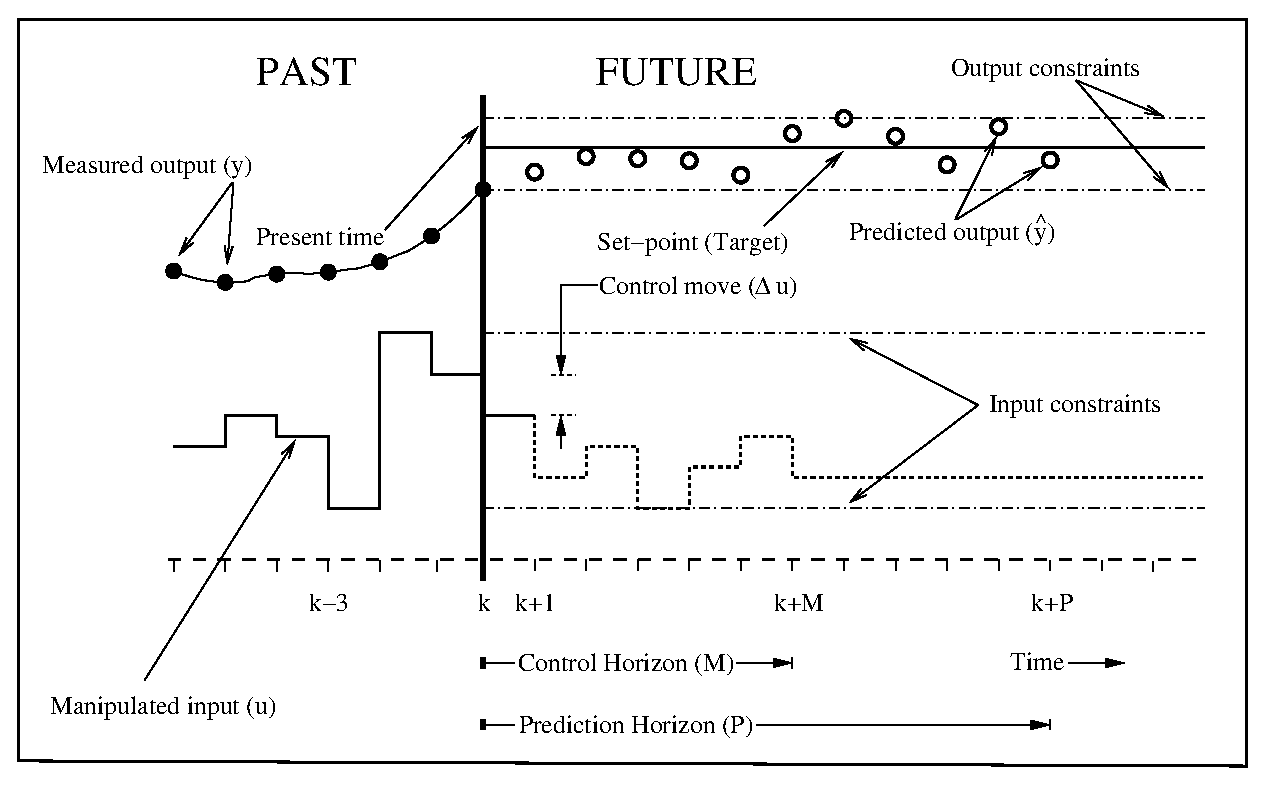
\includegraphics[width=5in]{mpc.eps}
\end{center}
\caption{Schematic illustrating receding horizon control. \label{fig:mpc-2}}
\end{figure}

\renewcommand{\baselinestretch}{2}
\large\normalsize

This does not necessarily mean that the text before and after the figure will be exactly what you want.  Remember Latex will place the figure where it will fit on the page the best.   The previous figure is Figs.~\ref{fig:mpc-2}. 

\section{Wrapping Text around Figure}


\renewcommand{\baselinestretch}{1}
\begin{wrapfigure}{r}{0.4\textwidth}
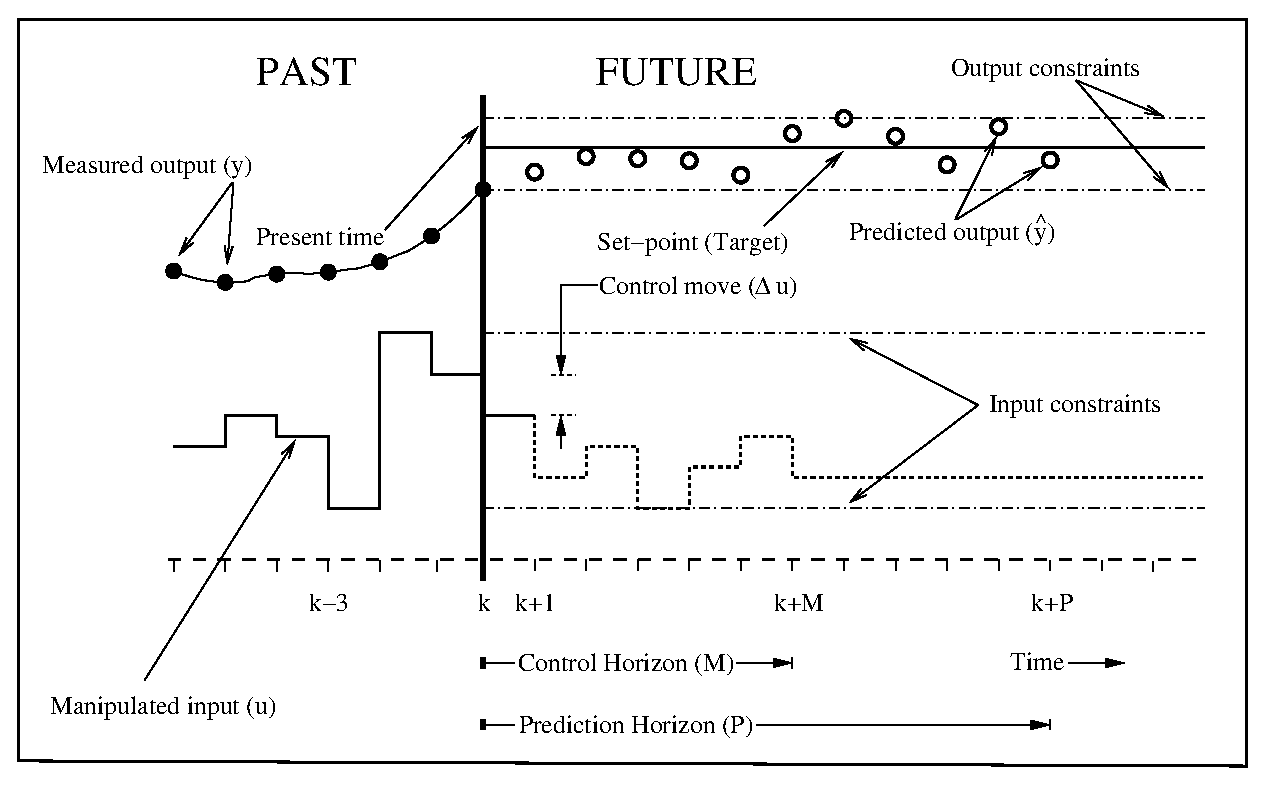
\includegraphics[width=0.4\textwidth]{mpc.eps}
\caption{ Text wrap around figure. \label{fig:test}}
\end{wrapfigure}

\renewcommand{\baselinestretch}{2}
\large\normalsize

By way of summary, at the end of the activity, I reminded the class of what we'd done:  by considering relatively nearby galaxies whose distance we had measured by some other means, we were able to establish a relationship locally between redshift and distance.  
By way of summary, at the end of the activity, I reminded the class of what we'd done:  by considering relatively nearby galaxies whose distance we had measured by some other means, we were able to establish a relationship locally between redshift and distance.  
By way of summary, at the end of the activity, I reminded the class of what we'd done:  by considering relatively nearby galaxies whose distance we had measured by some other means, we were able to establish a relationship locally between redshift and distance.  
By way of summary, at the end of the activity, I reminded the class of what we'd done:  by considering relatively nearby galaxies whose distance we had measured by some other means, we were able to establish a relationship locally between redshift and distance.  See Fig.~\ref{fig:test}.


\section{LaTeX -- A Typesetting Program}

A 13-page explanation of some of the features of LaTeX can be downloaded from http://www.jgsee.kmutt.ac.th/exell/General/LaTeX.html.


\section{Using Bibtex}

Using Bibtex with Latex documents is not difficult.  The bulk of the work is organizing your bibtex file, which is a data base compiled by you of the articles, books, etc. which you use in the bibliographies or reference sections of your publications.  

I have linked several files to this webpage, which will be helpful when you are using Bibtex.  These files can be downloaded from \newline
http://www.ireap.umd.edu/ireap/theses/bibtex.  Please read the file "BibtexInstructions.pdf".  The first two pages explain how to set up and run Bibtex; the remaining pages were taken from a published article and show how the references were cited in the .tex file.   The files BibtexInstructions.tex, Galactic.bib, Dottie.bib are the original .tex files used for BibtexInstructions.pdf.  The file BibtexSamples.tex contains examples of the information needed for the various publications you wish to reference (e.g., articles in refereed journals, books, unpublished articles, conference proceedings, etc.).

If you have questions concerning Bibtex, please contact me at 301-405-4955 or dbrosius at umd.edu.

\section{Using Natbib}

Another option of citing references in the bibliography is using Natbib instead of Bibtex.  You must still create a bibtex file, as noted above.  The command "backslash cite" cannot be used with natbib; instead "backslash citet" and "backslash citep" must be used.    "backslash citet" is used to show reference in the text (e.g., Eq.\ 8 in Reiser,1996 shows ...); "backslash citep" is used in the parenthetical (e.g., Eq.\ 8 (Reiser, 1996) shows ...).  

\begin{verbatim}
Add in preamble -- \usepackage[option]{natbib} 

Add at bottom of mainthesis.tex file --
\bibliography{name of your bibtex file}
\bibliographystyle{plainnat, abbrnat, or unsrtnat}
\end{verbatim}

Typesetting:   Latex, Bibtex, Latex, Latex

The reference sheet for natbib usage can be found at \newline "http://merkel.zoneo.net/Latex/natbib.php".

\section{APS Physical Review Style and Notation Guide}

The following style guide may be downloaded from The American Physical Society at http://forms.aps.org/author/styleguide.pdf:  Physical Review Style and Notation Guide, published by The American Physical Society, compiled and edited by Anne Waldron, Peggy Judd, and Valerie Miller, February 1993.  It may be old, but it is very useful.


			% !TEX root = mainthesis.tex
%Chapter 2

\renewcommand{\thechapter}{2}

\chapter{Basic theory of Bose-Einstein condensation}

Bose-Einstein condensation (BEC) is a quantum state of mater in which particles with integer valued spin all tend to occupy or `condense' into the ground state. In dilute gases, condensation occurs when the temperature of the system goes bellow a critical temperature where the bosons become indistinguishable particles and quantum statistics become relevant. 

BECs enable the observation of macroscopic quantum phenomena and there have been a number of fascinating experiments studying the properties of this systems, from measuring interference fringes from a macroscopic wave function to studying collective effects such as the propagation of sound~\cite{ketterle_w._making_1999}, as well as extensive theoretical developments~\cite{dalfovo_theory_1999}. In our experiments however BECs are not the primary object of study, instead they are used as the platform for performing quantum simulations. 

In this Chapter I describe the basic properties of Bose-Einstein condensation in dilute atomic gases. First I will describe the case of an ideal gas and then consider the effects of interactions and a trapping potential. A reader interested in learning about this subject in more depth is advised to read~\cite{Pethick} and~\cite{noauthor_bose-einstein_2003}.

\section{Bose-Einstein condensation of an ideal gas}

At low temperatures and in thermodynamic equilibrium, the mean occupation number of non-interacting identical bosons occupying the state with energy $E$ is given by the Bose distribution
%
\begin{equation}
	n(E_j)=\frac{1}{e^{(E_j-\mu)/k_BT}-1}
	\label{eq:Bose_distribution}	
\end{equation}
%
where $T$ is the temperature, $\mu$ is the chemical potential (the energy cost of adding or removing a particle) and $k_B$ is the Boltzmann constant. In the limit of large temperatures the Bose distribution can be approximated by the Maxwell-Boltzmann distribution
%
\begin{equation}
	n(E_j)\approx e^{-(E_j-\mu)/kT}
\end{equation}
%
which applies to classical, distinguishable particles. The chemical potential is determined by the condition that the total number of particles $N$ is equal to the sum over all states in the distribution $N=\sum_jn(E_j)$ and is therefore a function of $N$ and $T$. Additionally, in order for $n(E_j)$ to be positive definite we must have $\mu\leq E_0$ where $E_0$ is the energy of the ground state. From the Bose distribution we can see that the occupation number of the ground state is unbounded when $\mu\rightarrow0$. As shown in Figure \note{TODO: make figure of Bose distribution} the temperature decreases the occupation number in the ground state increases until all atoms collapse into the lowest energy level and Bose condense. 

\subsection{Critical temperature}
Now I will derive an analytical expression for the critical temperature at which atoms condense. For closely spaced energy levels (compared to $k_B T$) the sum representing the total number of particles can be replaced by the integral
%
\begin{equation}
	N=\int_0^\infty n(E) g(E) dE
	\label{eq:N(E)}
\end{equation}
%
where $g(E)$ is the density of states and $g(E)dE$ corresponds to the number of available states with energy between $E$ and $E+dE$. For a free particle in three dimensions the density of states is
%
\begin{equation}
	g(E)=\frac{V m^{3/2}}{\sqrt{2}\pi^2\hbar^2}E^{1/2},
	\label{eq:free_particle_dos}
\end{equation}
%
and in general the density of states can be expressed as a power of energy $g(E)=C_\alpha E^{\alpha-1}$. 

The integral in Equation~\ref{eq:N(E)} is not analytically solvable, however we can make the simplifying assumption $\mu=0$. The critical temperature $T_c$ is determined by the condition that all particles are in the excited states
%
\begin{align}
	N&=N_{\rm{ex}}(T_c, \mu=0) \nonumber \\
	&=\int_0^{\infty}\frac{g(E)dE}{e^{E/k_BT_c}-1} \nonumber \\
	&= C_\alpha(k_BT_c)^\alpha\int_0^\infty\frac{x^{\alpha-1}}{e^x-1} \nonumber \\
	&= c_\alpha (k_BT_c)^\alpha\Gamma(\alpha)\zeta(\alpha)
	\label{eq:finding_Tc}
\end{align}
%
where I made the substitution $x=E/k_BT_c$, $\Gamma(\alpha)=\int_0^\infty x^{\alpha-1}e^{-x}dx$ is the Gamma function and $\zeta(\alpha)=\sum_{n=1}^\infty n^{-\alpha}$ is the Riemann zeta function. From Equation~\ref{eq:finding_Tc} we find that the critical temperature for Bose-Einstein condensation is
%
\begin{equation}
	k_BT_c=\left(\frac{N}{C_\alpha\Gamma(\alpha)\zeta(\alpha)}\right)^{1/\alpha}.
\end{equation}

As mentioned earlier, Bose-Einstein condensation can be understood in terms of the de Broglie waves associated to particles. The thermal de Broglie wavelength is defined as
%
\begin{equation}
	\lambda_{\rm{th}}=\left(\frac{2\pi\hbar^2}{mk_BT}\right)^{1/2}
\end{equation}
%
and it characterized the spatial extension of the wave packet an individual particle at temperature $T$. Condensation occurs when $\lambda_{\rm{th}}$ becomes comparable with the inter-particle separation $n^{-1/3}$, where $n=N/V$. Using the density of states for a free particle in 3D (Equation~\ref{eq:free_particle_dos})in combination with the expression for the critical temperature (Equation~\ref{eq:finding_Tc}) we find that indeed when $T=T_c$
%
\begin{equation}
	n\lambda_{\rm {th}}^3=\zeta\left(\frac{3}{2}\right)\approx 2.612
\end{equation}
%
both quantities are comparable. The quantity $n\lambda_{\rm{th}}^3$ is known as the phase space density which describes the number of particles contained in a box with volume $\lambda_{\rm{th}}^3$. In order to experimentally produce BECs, a combination of laser and evaporative cooling techniques are deployed such that we can increase the density while minimizing the temperature and therefore maximize the phase space density. The densities for BECs of Alkali atoms typically range in of order $10^{13}$ to $10^{15}$ atoms/cm$^{-3}$.

\subsection{Condensate fraction}

Now we look at the fraction of particles occupying the ground state at temperatures below $T_c$. The total number of particles is given by $N=N_0+N_{\rm{ex}}$. The number of particles in the excited state will be given by the integral in Equation~\ref{eq:N(E)}. For $g(E)=C_\alpha E^{\alpha-1}$and  $\alpha>0$ the integral converges and we get
%
\begin{align}
	N_{\rm{ex}}&=c_\alpha (k_BT)^\alpha\Gamma(\alpha)\zeta(\alpha) \nonumber \\
	&=N\left(\frac{T}{T_c}\right)^\alpha,
\end{align}
%
where I used the expression for the total number of particles at $T_c$ from Equation~\ref{eq:finding_Tc}. The number of particles in the ground state is therefore
%
\begin{align}
	N_0&=N-N_{\rm{ex}} \nonumber \\
	&= N\left[1-\left(\frac{T}{T_c}\right)^\alpha\right]
\end{align}

\subsection{Bose gas in a harmonic trapping potential}

I consider the particular case of particles confined in a three dimensional harmonic potential
%
\begin{equation}
V(\r)=\frac{m}{2}\left(\omega_x^2x^2+\omega_y^2y^2+\omega_z^2z^2\right)
\label{eq:ho}
\end{equation}
%
as it is the most relevant to our experiments that are performed in harmonic traps. The density of states is given by 

\begin{equation}
	g(E)=\frac{E^2}{2\hbar^2\omega_x\omega_y\omega_z},
\end{equation}
%
which corresponds to $\alpha=3$ and $C_3=(2\hbar^3\omega_x\omega_y\omega_z)^{-1}$. Using Equation~\ref{eq:finding_Tc}, the transition temperature is
%
\begin{equation}
 	k_B T_c=\frac{\hbar \bar{\omega}N^{1/3}}{\zeta(3)^{1/3}}\approx0.94\hbar\bar{\omega}N^{1/3}
 \end{equation} 
%
where $\bar{\omega}=(\omega_x\omega_y\omega_z)^{1/3}$ is the geometric mean of the oscillation frequencies. Similarly we find that the condensed fraction is
%
\begin{equation}
	N_0=N\left[1-\left(\frac{T}{T_c}\right)^3\right]
\end{equation}

Condensates in harmonic traps have some striking features that will be further explored in more detail in the following sections. The confining potential makes the BECs both finite sized and inhomogeneous which means that the BEC can be observed both in momentum space and in coordinate space. Another consequence of the inhomogeneity of these systems is the role of two-body interactions, which gets enhanced and leads to noticeable effects in measurable quantities (see~\cite{dalfovo_theory_1999,castin_bose-einstein_1996}).

\section{Bose-Einstein condensation with atomic interactions}

Even though atomic BECs are made from very dilute gases, the system is far from being an ideal gas and interactions need to be taken into account for a complete treatment of the system. 

The collisional properties of particles at low energies, such as cold atoms in a condensate, are dominated by $s$-wave scattering which can be described in terms of a single parameter the scattering length $a$ that determines both the scattering cross section $\sigma=4\pi a^2$ and the . 

The magnitude of the scattering length is determined by the interatomic interaction potentials. For Alkali atoms at large distances, the two-body interactions are dominated by an attractive Van der walls interaction $U(r)=-C_6/r^6$ that arises from dipole-dipole interactions. At smaller distances the attractive potential is replaced by a strong repulsive electron-exchange interaction. This minimal model captures the most important properties of the inter-atomic potential and can be solved analytically~\cite{gribakin_calculation_1993}. 

If the range of the interaction is much shorter than the mean inter-atomic distance the interaction can be approximated by an effective pseudo-potential $U_{\rm{eff}}(\r-\r')$ such that
%
\begin{equation}
	a=\frac{m}{4\pi\hbar^2}\int U_{\rm{eff}}(\r-\r')d \r
\end{equation}
%
which determines
%
\begin{equation}
	U_{\rm{eff}}(\r-\r')=\frac{4\pi\hbar^2a}{m}\delta(\r-\r')=g\delta(\r-\r').
\end{equation}
%
This is a nice approximation as it allows us to model the scattering between atoms as a hard sphere scattering process instead of considering the more complicated inter-atomic potentials. The sign of the scattering length determines the attractive or repulsive nature of the interactions and it  plays an important role in the experimental production of BECs as it determines the rate at which atoms thermalize during evaporative cooling.  For  $\Rb87$ at zero magnetic field $a=103 a_0$ where $a_0=\unit[5.29\times10^{-11}]{m}$ is the Bohr radius while for the more abundant isotope $^85$Rb $a=-\unit[23.44]{nm}$ which means that a BEC with density beyond a critical value can collapse~\cite{gerton_direct_2000}. \note{TODO: try to find references for the values of scattering lengths}

\subsection{Gross-Pitaevskii equation}

The effective Hamiltonian describing $N$ identical bosons with contact interactions can be written as
%
\begin{equation}
	\hat{H}=\sum_{i=1}^N\left[\frac{\mathbf{p}_i^2}{2m}+V(\r_i)\right]+g\sum_{i<j}\delta(\r_i-\r_j),
	\label{eq:many_body_h}
\end{equation}
%
where $V(\r)$ is an external potential and $\mathbf{p}_i=-i\hbar\nabla_i$. We now consider a normalized eigenstate of the Hamiltonian $\Psi(\r_1, \r_2, ..., \r_N)$. We can simplify this state by taking a mean field approach. If we assume that the system has undergone condensation so that the majority of the particles share the same single particle ground state $\psi_0(\r)$ the wavefunction can be approximated by a symmetrized product
%
\begin{equation}
	\Psi(\r_1, \r_2, ..., \r_N)=\prod_{i=1}^N\phi(\r_i),
	\label{eq:mean_field_psi}
\end{equation}
%
where $\psi_0$ is normalized to unity. The energy of the state from Equation~\ref{eq:mean_field_psi} is given by the expectation value
%
\begin{align}
	E&=\int\Psi^*\hat{H}\Psi \,d\r \nonumber \\
	&=N\int\left[-\frac{\hbar^2}{2m}\vert \nabla\phi(\r)\vert^2+V(\r)\vert\phi(\r)\vert^2+\frac{(N-1)}{2}g\vert \phi(\r)\vert^4\right]d\r,
	\label{eq:mean_field_E}
\end{align}
%
where $N(N-1)/2\approx N^2/2$ is counting the number of terms in the interaction energy. Now we introduce the wave function of the condensate $\psi(\r)=N^{1/2}\phi(\r)$, which when inserted in Equation~\ref{eq:mean_field_E} makes the $N$ factors disappear. The optimal form of $\psi$ should minimize the energy subject to the normalization condition $N=\int\vert\psi(\r)\vert^2\,d\r$. This can be done by introducing a Lagrange multiplier $\mu$
%
\begin{align}
	\frac{\delta}{\delta \psi^*(\r)}\left(E-\mu\int\vert\psi\vert^2\,d\r \right) 
	&= \left[-\frac{\hbar^2}{2m}\nabla^2+V(\r)+g\vert\psi(\r)\vert^2-\mu\right]\psi(\r)
	=0
\end{align}
%
and we thus find that the condensate wave function obeys a non-linear Schr\"odinger equation known as the Gross-Pitaevskii (GP) equation
\footnote{The GP equation is very minimally relevant to my experiment but it still feels good knowing where it comes from.}.  
%
\begin{equation}
	\left[-\frac{\hbar^2}{2m}\nabla^2+V(\r)+g\vert\psi(\r)\vert^2\right]\psi(\r)=\mu\psi(\r)
\end{equation}
%
where $\mu$ plays the role of the chemical potential. The dynamics of the condensate will similarly be described by the time-dependent GP equation
%
\begin{equation}
	i\hbar\frac{\partial}{\partial t}\psi(\r,t)=\left[-\frac{\hbar^2}{2m}+V(\r)+g\vert\psi(\r,t)\vert^2\right]\psi(\r,t)
\end{equation}

The GP equation describing the relevant phenomena associated
with BECs, for example the propagation of collective excitations and the expansion of the condensate when released from a trap. The crucial assumption when deriving these equations was the mean field approximation which should be valid for dilute BECs in which the condensate fraction is close to unity. The excitations of the system (deviations from the mean field) can be treated using Bogoliubov theory for weakly interacting bosons\cite{Pethick}. 

\subsection{Thomas-Fermi approximation}

For systems with large $N$, the interaction term in the GP equation is very large compared to the kinetic energy\footnote{It can be shown that the ratio of kinetic energy to interactions scales like $N^{-4/5}$}. As the kinetic energy becomes less important we enter the Thomas-Fermi (TF) regime where the energy of the system is given only by the external potential and the mean field energy and the GP equation is considerably simplified 
%
\begin{equation}
	\left[V(\r)+g\vert\psi(\r)\vert\psi(\r)\vert^2\right]\psi(\r)=\mu\psi(\r).
\end{equation}
%

In the TF regime the density distribution of the condensate $n(\r)=\vert\psi(\r)\vert^2$ reflects the shape of the external potential
%
\begin{equation}
	n(\r)=g^{-1}[\mu-V(\r)],
\end{equation}
%
when $\mu-V(\r)>0$ and is otherwise zero. For a harmonic confining potential (Equation~\ref{eq:ho}) as is typical in our experiments we find that the length scale that characterizes the size of the condensate is the Thomas-Fermi radius
%
\begin{equation}
	R_j=\sqrt{\frac{2\mu}{m\omega_j^2}}, \ \ \ j=x,y,z.
\end{equation}
%
The density of the condensate is described by an inverted parabola
%
\begin{equation}
	n(\r)=\frac{\mu}{g}\left(1-\frac{x^2}{R_x^2}-\frac{y^2}{R_y^2}-\frac{z^2}{R_z^2}\right).
	\label{eq:n_tf}
\end{equation}
 %
 
By integrating over Equation~\ref{eq:n_tf} we find that
 %
 \begin{equation}
 	N=\frac{8\pi}{15}\frac{\mu}{g}R_xR_yR_z,
 \end{equation}
 %
 which is a useful quantity for determining the number of atoms in the condensate based on density profiles. In practice our images are taken after the atoms are released from the trap and the density profile is modified due to interactions. This will be discussed in more detail in the next following section. 

\section{Density distributions}

Most ultracold atoms experiments are probed by directly imaging the atoms (e.g. with absorption imaging, Section~\ref{sec:absorption imaging}). If the atoms are imaged in-situ we gain access to their spatial density profiles. If the atoms are released from the trap and allowed to expand in time of flight (TOF) we can measure their momentum distribution. In this section I summarize the signatures in the density distributions of BECs and thermal atoms confined in a harmonic potential both in-situ and after TOF. 

For a thermal gas in a harmonic potential at temperatures higher than the level spacing $k_BT>\hbar\omega_{x,y,z}$ the density is given by~\cite{ketterle_w._making_1999}
%
\begin{equation}
	n_{\rm{th}}(\r)=\frac{1}{\lambda_{\rm{th}}^3}g_{3/2}(z(\r))
\end{equation}
%
where $z(\r)=\exp(\mu-V(\r)/\k_BT$, $V(\r)$ is given by Equation~\ref{eq:ho}, $\mu$ is the chemical potential and $g_j(z)=\sum_iz^i/i^j$ is the Bose function. The Bose function introduces effects of quantum statistics and compared to a distribution of distinguishable particles, the peak density of a Bose gas is increased by $g_{3/2}(z)/z$, a phenomenon known as Bose-enhancement.

The distribution after TOF can be calculated considering that the trapped atoms fly ballistically from their position in the trap. An atom starting initially at the point $\r_0$ moves to the point $\r$ after a time $t$ if its momentum is given by $\mathbf{p}=m(\r-\r0)/t$, and it can be shown that
%
\begin{align}
	n_{\rm{tof}}&=\frac{1}{\lambda_{\rm{th}}}\prod_{i=1}^3g_{3/2}\left(\exp\left[\mu-\frac{m}{2}\sum_{i=1}^3x_i^2\left(\frac{\omega_i^2}{1+\omega_i^2t^2}\right)\right]\right) \nonumber \\
	&\approx \frac{1}{\lambda_{\rm{th}}}g_{3/2}\left(\exp\left[(\mu-\frac{mr^2}{2t^2})/k_BT\right]\right)
\end{align}
%
where the approximation in the second line is valid for $t\gg \omega_i^{-1}$. The temperature of the atoms can be estimated by looking at the wings of the density distribution after TOF. Even with the case of Bose enhancement, the density of the wings still decays exponentially as $\exp(-x_i^2/\sigma_i^2)$ and the temperature of the cloud can be determined using
%
\begin{align}
	k_BT&=\frac{m}{2}\left(\frac{\omega_i^2}{1+\omega_i^2t^2}\sigma_i^2\right) \nonumber \\
	&\approx \frac{m}{2}\left(\frac{\sigma_i}{t}\right)^2
\end{align}

For the case of a BEC at zero temperature (no thermal fraction) the in-situ density distribution is described by the Thomas-Fermi distribution 
%
\begin{align}
	n(\r)&=n_0\left(1-\frac{x^2}{R_x^2}-\frac{y^2}{R_y^2}-\frac{z^2}{R_z^2}\right) \nonumber \\  
	&= \frac{15N}{8\pi R_xR_yR_z}\left(1-\frac{x^2}{R_x^2}-\frac{y^2}{R_y^2}-\frac{z^2}{R_z^2}\right) .
\end{align}

Even though the BEC is in the motional ground state, it will expand during TOF as a consequence of interactions. The expansion can be determined using the time dependent GP equation. A detail account of the procedure can be found in \cite{castin_bose-einstein_1996}, the procedure relies on using the ansatz that the TF radii expand as
%
\begin{equation}
	R_i(t)=\lambda_i(t)R_i(t=0),
	\label{eq:castin_dum_radius}
\end{equation}
%
where I assumed that the condensate is in the trap at $t=0$ which implies that $\lambda_i(0)=1$. If the trap is suddenly turned off at $t>0$ from inserting the TF wave function with radii given by Equation~\ref{eq:castin_dum_radius} into the time-dependent GP equation we find a series differential equations
%
\begin{equation}
	\frac{d^2\lambda_i}{dt^2}=\frac{\omega_i^2}{\lambda_i\lambda_x\lambda_y\lambda_z}
\end{equation}
%
which can be used to determine the density profile of the BEC in TOF. Alternatively if the density profile of the BEC is known from an image, these relations can used to back-propagate what the original TF radii of the confined condensate was. 

For partially condensed clouds the density profiles will be given by a combination of the thermal density profiles and the Thomas-Fermi density profile. 




% were when the condensate
% was confined.
% or by measuring the
% TOF radii via absorption imaging, back-propagate what the original radii were when the condensate
% was confined.
% %
% \begin{align}
% 	n(\r)&=n_0e^{-(\frac{x^2}{2\sigma_x^2}+\frac{y^2}{2\sigma_y^2}+\frac{z^2}{2\sigma_z^2})}\nonumber \\
% 	&= \frac{15N}{8\pi R_xR_yR_z},
% \end{align}
% %
% where $\sigma_i=\omega_i^{-1}\sqrt{k_BT/m}$. Using the equipartition theorem we find that the spatial extension of the cloud and the temperature are related by 
% %
% \begin{equation}
% 	T=\frac{m}{k_B}\sigma_i^2\omega_i^2
% \end{equation}

% \note{TODO: what is my chemical potential?}


% For a given trapping potential $U(\r)$, the density distribution of a thermal ensamble is
% \begin{equation}
% 	n(\r) = n_0 e^{-\frac{U(\r)}{k_BT}}.
% \end{equation}
% %
% The temperature $T$ can be derived from the density distribution. For a 3D harmonic trap


			% !TEX root = mainthesis.tex

%Chapter 3


\renewcommand{\thechapter}{3}

\chapter{Manipulation and detection of ultra-cold atoms}
\label{ch:Ch3}

All of the experiments described in this thesis were performed using ultracold clouds of $\Rb87$. Both the cooling and trapping of atoms as well as the engineering of interesting potentials and detection of atoms rely on the interaction of atoms with electromagnetic fields as well as with static and oscillating magnetic fields. 

In this Chapter I describe the techniques and interactions that make our experiments possible. This Chapter is not meant to be an extensive survey of atomic physics but rather covers the topics that are most relevant to the experiments presented in this thesis. The references I included are helpful if the reader is interested in the details of the derivations or wants to expand on a given topic. I start by describing the electronic structure of $\Rb87$. Then I review the interactions of atoms with magnetic fields which allows us to shift the energies of different atomic states. I describe the foundations of atom-light interactions that make possible both laser cooling and trapping of atoms and gives rise to Raman induced transitions. Finally I discuss the absorption imaging technique that we use to detect atoms after all our experiments are performed. 

\section{Electronic structure of $^{87}$Rb}
\label{sec:electronic_structure}

Rb is an Alkali metal (also Li, which exists in our vacuum chamber but was never used). Alkali metals correspond to the first group (leftmost column) of the periodic table and are characterized by having a single valence electron, which makes the description of their internal structure much simpler than that of other elements. We can describe the state of an electron in an atom by its angular momentum $\mathbf{\hat{L}}$ and its spin $\mathbf{\hat S}$. Because of Pauli's exclusion principle there can not be two electrons with the same quantum numbers and in multi-electron atoms they tend to fill `shells' of different angular momentum values, historically labeled by the letters $S,\ P,\ D,\ F,\ ...$\footnote{This terms were used to describe the lines in the emission spectra when they were first discovered. $S$ stands for sharp, $P$ for principal $D$ for diffuse and $F$ for further noted} (corresponding to $L=1,\ 2,\ 3,\ 4,\ ...$). In particular Rb has 4 filled shells and one electron in the $5S$ 
shell, where the number $5$ corresponds to the principal quantum number $n$. Figure \note{TODO: make figure of atomic energy levels} shows the energy levels of the ground state $5S$ and its closest $5P$ orbital. %In the absence of interactions, the $m_l$ sublevels within an orbital are degenerate.

The atomic level structure is modified by relativistic effects. In particular the relativistic treatment of the electron's motion gives rise to an interaction between the electron's intrinsic magnetic moment (the spin) $\mathbf{\hat S}$ and the orbital angular momentum $\mathbf{\hat L}$. This spin-orbit coupling interaction $\hat H_{\rm {fs}} \propto \mathbf{L}\cdot\mathbf{S}$ causes the fine structure splitting of the electronic orbitals into levels with different total electronic angular momentum $\mathbf{J}=\mathbf{\hat L}\cdot\mathbf{\hat S}$. Figure~\ref{fig:fs_hfs}b show the $5^2S_{1/2}$, $5^2P_{1/2}$ and $5^2P{3/2}$ electronic configurations that arise from this splitting, where the subscript indicates the value of $J$. For $S$ ($L=0$) orbitals $J=1/2$ is the only possible value and the levels are not split. For the $P$ orbital ($L=1$) $J$ and a single electron with $S=1/2$, $J$ can be $1/2$ or $3/2$ and the $P$ orbital splits into two levels. The $5S_{1/2}\rightarrow 5P_{1/2}$ is known as the D1 line and has wavelength $\lambda=\unit[794.979]{nm}$ and $5S_{1/2}\rightarrow 5P_{3/2}$ transition is known as the D2 line and has $\lambda=\unit[790.241]{nm}$ \cite{Steck}. 

The atomic level structure gets further modified by the magnetic interaction of the electronic magnetic flux density with the nuclear spin $\mathbf{I}$. This is another kind of spin-orbit interaction that gives rise to the hyperfine splitting of the atomic levels which can be described by the Hamiltonian $\hat H_{\rm{hfs}} = A_{\rm{hfs}}\mathbf{I}\cdot\mathbf{J}$. A complete derivation of $\hat H_{\rm{hfs}}$ can be found in~\cite{schwartz_theory_1955}. The hyperfine levels correspond to different values of the total angular momentum $\hat F=\hat J+\hat I$. For $\Rb87$ $I=3/2$~\cite{Steck} which results in the level structure shown in Figure~\ref{fig:fs_hfs}c 

\note{TODO: talk about cooling and repumping transitions which is relevant for the absorption imaging section.}

\section{Interaction between atoms and magnetic fields}
\label{sec:zeeman_effect}

Atoms have have an intrinsic magnetic moment that is given by the sum of nuclear and electronic moments
%
\begin{equation}
	\boldsymbol{\hat \mu}=-\frac{g_J\mu_B}{\hbar} \mathbf{\hat J}+\frac{g_I\mu_N}{\hbar}\mathbf{\hat I}=\frac{\mu_B g_F}{\hbar} \mathbf{\hat F}
\end{equation}
%
where $\mu_B$ is the Bohr magneton, $\mu_N$ \footnote{$\mu_N\ll\mu_B$ and therefore $\boldsymbol{\hat \mu}\approx-\mu_Bg_J/\hbar\mathbf{\hat J}$} is the nuclear magneton and $g_J$, $g_I$ and $g_F$ are the Land\'e $g$-factors corresponding to the electronic, nuclear and total angular momentum. In the presence of an external magnetic field $\mathbf B$, the internal levels of an atom get modified due to the Zeeman~\cite{Zeeman_effect} interaction
%
\begin{equation}
	\hat{H}_{\rm{Zeeman}}=-\boldsymbol{\hat \mu}\cdot\mathbf{B}
	\label{eq:zeeman_hamiltonian}
\end{equation}
%
which has the effect of lifting the degeneracy of the different $m_F$ states. We take advantage of this effect for making (state-dependent) magnetic traps for the atoms by using magnetic field gradients and for the experiments presented in Chapters~\ref{ch:Fourier_spectroscopy},~\ref{ch:clock_states} and \ref{ch:Rashba} the shifts in the $m_F$ energies allowed us to treat each state as a pseudospin that we then coherently manipulated using the techniques described in Section~\ref{sec:quantum_coherent_dynamics}.

The total energy shifts are calculated by diagonalizing the full atomic Hamiltonian including the fine and hyperfine structure terms. For a small magnetic field the Zeeman term can be treated as a perturbation and the energy split is linear with the magnitude of the field $\Delta E_{\rm{Zeeman}}=g_F\mu_B m_FB$, what is known as the `linear Zeeman regime' where $F$ and $m_F$ are good quantum numbers. In contrast, in the `Pachen-Back regime' large magnetic fields the Zeeman term dominates over the fine and hyperfine terms and therefore the good quantum numbers of the system are $J$ and $m_J$. Our experiments typically operate in an intermediate regime ($B\sim 10-30\,\rm{G}$)energies where the magnetic field and as a result the energy of $m_F=0$ gets a small shift in energy that is quadratic in $B$. For atoms in $F=1$ we define this quadratic Zeeman shift as $\epsilon=E_0-(E_{+1}-E_{-1})/2$, where $E_{m_F}$ is the Zeeman shift for state $m_F$.

For the particular case of $J=1/2$ (like the ground state of Alkalis) the Zeeman energies can be found analytically using the Breit-Rabi formula~\cite{breit_measurement_1931}
%
\begin{equation}
	E_{m_F}=-\frac{1}{2(2I+1)}+\frac{\mu_Bg_Im_FB}{\Delta E_{\rm{hf}}}+\frac{1}{2}\sqrt{1+\frac{4m_F}{2I+1}x+x^2},
	\label{eq:Breit_rabi}
\end{equation}
%
where $\Delta E_{\rm{hf}}=A_{\rm{hf}}(J+1/2)$ and $x=(g_J-g_I)\mu_B B_z/\Delta E_{\rm{hf}}$. Figure \note{TODO:make figure} shows the energies of the $m_F$ levels for the $F=1$ and $F=2$ manifolds of $\Rb87$.

\section{Interaction between atoms and electric fields}
\label{sec:atom-lignt_interactio n}

In this section I will discuss the interaction between atoms and electromagnetic radiation (light). After laying the foundations I will discuss applications using off-resonant light such as optical dipole traps and Raman transitions. I will not cover laser cooling which has been covered extensively in the literature~\cite{metcalf_deceleration_1999,phillips_nobel_1998} and PhD theses from previous lab members~\cite{CampbellThesis,PriceThesis}. 

In the presence of an electric field $\mathbf E$ an atom can become polarized and therefore its energy levels get modified by the Stark effect~\cite{stark_beobachtungen_1914}. If the electric field is spatially uniform with respect to the atom's size we consider the electric field as a classical object and its effect on the atom can be described by the the Hamiltonian~\cite{Cohen-Tanoudji}  
%
\begin{equation}
\hat{H}_{\rm{dip}} = -\mathbf{\hat d}\cdot\mathbf{E},
\label{eq:dipole_ham}	
\end{equation}
%
where $\mathbf{\hat d}=-e\sum_j r_j$ is the atomic dipole operator, $e$ is the electron charge and $\hat r_j$ are the position operators of the atom's electrons relative to the center of mas of the atom. This approximation, known as the dipole approximation, is valid for electromagnetic radiation when the wavelength is much larger than the size of an atom $\lambda\gg r_{\rm{atom}}$~\cite{SteckTextbook}. 

For a coherent electromagnetic field $\mathbf{E}(\omega,t)$ with angular frequency $\omega$, the dipole Hamiltonian can be written in terms of a dynamic polarizability
%
\begin{equation}
	\hat{H}_{\rm{dip}}=-\alpha_{\mu\nu}(\omega)E_{\mu}^{(+)}E_{\nu}^{(-)}
\end{equation}
%
where $\mathbf{E}^{(\pm)}$ are the possitive/negative frequency components of the field. $\alpha_{\mu\nu}(\omega)$ can be found by looking at the (time averaged) shift in the energy of the a given state state using second order time-dependent perturbation theory~\cite{SteckTextbook,deutsch_quantum_2010}. For the ground state $\ket{g}$ the polarizability takes the form
%
\begin{equation}
	\alpha_{\mu\nu}(\omega)=\sum_j\frac{2\omega_{jg}\bra{g}d_\mu\ket{e_j}\bra{e_j}d_\nu\ket{e_j}}{\hbar(\omega_{jg}^2-\omega^2)},
\end{equation}
%
where $\ket{e_j}$ represent the excited states and $\omega_{jg}=(E_j-E_g)/\hbar$. The dipole operator is a rank-1 tensor and can be represented by 3 irreducible tensor operators\footnote{A rank $k$ tensor can be represented by $2k+1$ irreducible tensor operators, which are collection of operators that transforms under
rotations like the spherical harmonics $Y_{kq}(\theta, \phi)$} (see~\cite{SteckTextbook} for a complete derivation). In the limit of small magnetic fields so that $F$ and $m_F$ are good quantum numbers describing the state of the atom $\ket{n, F, m_F}$ the dipole Hamiltonian in this representation takes a convenient form
%
\begin{align}
	\hat{H}_{\rm{dip}}= &\alpha^{(0)}(\omega)(\mathbf{E}^{(-)}\cdot\mathbf{E}^{(+)}) 
	+\alpha^{(1)}(\mathbf{E}^{(-)}\times\mathbf{E}^{(+)})\cdot\mathbf{\hat{F}}  \nonumber \\ 
	&+ \alpha^{(2)}E_i^{(-)}E_j^{(+)}	\left(\frac{1}{2}(F_iF_j+F_jF_i)-\frac{1}{3}\mathbf{\hat F}^2\delta_{i,j}\right)\Big],
	\label{eq:light_matter_coupling}
\end{align}
%
where $\alpha^{(0)}$, $\alpha^{(1)}$ and $\alpha^{(2)}$ are the scalar, vector and tensor polarizabilities respectively and $\hat{\mathbf{F}}$ is the total angular momentum operator. For all our experiments $\alpha^{(2)}$ is very small so I will limit the discussion to the effect of the first two terms. The scalar term is responsible for the dipole force that allow us to trap atoms using off-resonant light and the vector component is necessary for engineering spin-orbit coupling through Raman transitions and other spin-dependent potentials. 

\subsection{Scalar polarizability}
\label{sec:scalar_light_shift}

The scalar polarizability takes the form
%
\begin{equation}
	\alpha^{(0)}=\sum_j\frac{2\omega_{jg}\bra{g}\mathbf{d}\cdot\hat{\epsilon}\ket{e_j}\vert^2}{\hbar(\omega_{jg}^2-\omega^2)},
\end{equation}
%
where $\hat{\epsilon}$ represents the polarization vector of the light. The matrix element can be expressed in terms of the Clebsch-Gordan coefficients and the reduced matrix element using the Wigner-Eckart theorem~\cite{Sakurai}. For the ground state of an Alkali atom ($J=1/2$) the expression above gets simplified to
%
\begin{equation}
	\alpha^{(0)}\approx\sum_{J'}\frac{2\omega_{JJ'}\vert\langle J=1/2 \| \mathbf{d}\|J'\rangle\vert^2}{3\hbar(\omega_{JJ'}^2-\omega^2)}.
\end{equation}

The dipole matrix elements needed to compute the polarizability are related to the transition scattering rate via Fermi's golden rule~\cite{Sakurai,SteckTextbook}
\begin{equation}
	\Gamma_{JJ'}=\frac{\omega_{JJ'}^2}{3\pi\epsilon_0\hbar c^3}\frac{2J+1}{2J'+1}\vert\langle J \| \mathbf{d}\|J'\rangle\vert^2,
\end{equation}
%
and combining this with the expression for the intensity of the electric field $I(\r)=2\epsilon_0c\vert \mathbf{E}(\r)\vert^2$ it can be shown that for linearly polarized light the energy of the ground state manifold is shifted by
\begin{equation}
	U(\omega,\r)=-\frac{\pi c^2 I(\r)}{2}\left[ \frac{\Gamma_{\rm{D1}}}{\omega_{\rm{D1}}^2}\left(\frac{1}{\omega+\omega_{\rm{D1}}}-\frac{1}{\omega-\omega_{\rm{D1}}}\right)+\frac{2\Gamma_{\rm{D2}}}{\omega_{\rm{D2}}^2}\left(\frac{1}{\omega+\omega_{\rm{D2}}}-\frac{1}{\omega-\omega_{\rm{D2}}}\right)\right],
\end{equation}
%
where only the the most significant contribution from the closest transitions  (the D1 and D2 lines) are included. Here $U(\r)$ is related to the real part of the polarizability which is in fact a complex valued number. So far I have only considered the real part by assuming the excited states have an infinitely long lifetime. However, in reality the atom can spontaneously emit photons and decay. This exponential decay can be accounted for by adding an imaginary contribution to the energies $\omega_D\rightarrow\omega_D+i\Gamma_D\omega^3/\omega_D^3$ of the D1 and D2 transitions~\cite{grimm_optical_2000}. The scattering rate is related to the imaginary part of the polarizability and is given by
%
\begin{equation}
	\Gamma(\omega,\r)=\frac{\pi c^2I(\r)}{2\hbar}\left[ \frac{\Gamma_{\rm{D1}}\omega^3}{\omega_{\rm{D1}}^6}\left(\frac{1}{\omega+\omega_{\rm{D1}}}-\frac{1}{\omega-\omega_{\rm{D1}}}\right)^2+\frac{2\Gamma_{\rm{D2}}\omega^3}{\omega_{\rm{D2}}^6}\left(\frac{1}{\omega+\omega_{\rm{D2}}}-\frac{1}{\omega-\omega_{\rm{D2}}}\right)^2\right]
	\label{eq:scattering}
\end{equation}

The energy shift $U(\omega,\r)$ is a conservative term and is related to dipole trapping while the scattering term $\Gamma(\omega,\r)$ is dissipative and is important for laser cooling. In the context of engineering potentials for ultracold atoms with off-resonant light, the scattering is translated into heating because every time an atom emits a photon with angular frequency $\omega_L$ it gets a recoil momentum $\hbar\k_L$.  

If the frequency $\omega$ satisfies the relation $\omega+\omega_{\rm D}\gg\omega-\omega_{\rm D}$ we can neglect the terms proportional to $1/(\omega+\omega_{\rm D})$, an approximation typically known as the rotating wave approximation (RWA). If the RWA is valid then the frequency dependence of both the energy shifts and the scattering rates will be given by the detuning from the D1 and D2 transitions. 

\subsubsection{Optical trapping}
One important application of the scalar light-shift is to create optical traps for our clouds of ultracold atoms. The use optical fields with non-uniform spatial intensity can generate traps (and anti-traps) for the atoms which experience a force proportional to the intensity gradient $F_{\rm{dip}}=-\nabla U(\r)$.  \note{TODO: make nice figure of dipole trap?}. The production of BECs in our lab relies on the use of focused Gaussian laser beams with $\lambda=\unit[1064]{nm}$.  The intensity profile of a focused Gaussian beam propagating along $\ez$ is given by 
%
\begin{equation}
 	I(x,y,z) = \frac{2P}{\pi\omega^2(z)}e^{-\frac{x^2+y^2}{\omega^2(z)}}
 \end{equation} 
 %
 where $P$ is the total power of the beam and the $1/e^2$ radius is given by $w(z)=w_0\sqrt{1+z^2/z_R^2}$ where the minimum radius $w_0$ is known as the waist and $z_R=\pi\omega_0^2/\lambda$ is the Rayleleigh range. If the extent of an atomic cloud is small compared to the size of the beam we can perform a Taylor expansion around $\r=0$ to obtain the trapping potential
 %
 \begin{equation}
 	U(\r) = -U_0\left(1-2\frac{x^2+y^2}{\omega_0^2}-\frac{z^2}{z_R^2}\right).
 \end{equation}
%
The oscillation frequencies of the trap along the radial direction are $\omega_r=(4U_0/m\omega_0^2)^{1/2}$ and along the axial direction $\omega_z=(2U_0/mz_R)^{1/2}$. The beam waist is usually much smaller than the Rayleigh range ($\omega_0\sim \unit[50-150]{nm}$ for my experiments) and therefore the trap is much stronger along the axial direction. To get around this we use a `crossed dipole trap' which is formed by a combination of two cross-polarized\footnote{The beams are cross-polarized to avoid interference between them} focused Gaussian beams propagating along perpendicular axes, ensuring that we get good confinement of atoms along all spatial directions. 

For a given trapping potential $U(\r)$, the density distribution of a thermal ensamble is
\begin{equation}
	n(\r) = n_0 e^{-\frac{U(\r)}{k_BT}}.
\end{equation}
%
The temperature $T$ can be derived from the density distribution. For a 3D harmonic trap
%
\begin{equation}
	n(\r)=n_0e^{-(\frac{x^2}{2\sigma_x^2}+\frac{y^2}{2\sigma_y^2}+\frac{z^2}{2\sigma_z^2})},
\end{equation}
%
where $\sigma_i=\omega_i^{-1}\sqrt{k_BT/m}$. Using the equipartition theorem we find that the spatial extension of the cloud and the temperature are related by 
%
\begin{equation}
	T=\frac{m}{k_B}\sigma_i^2\omega_i^2
\end{equation}

\note{TODO: figure of dipole traps}

\note{TODO: talk about magic wavelength}

\subsection{Effective magnetic fields from vector polarizability}
\label{sec:}

Recall the Zeeman Hamiltonian introduced in Section~\ref{sec:zeeman_effect}. The term proportional to the vector polarizability in Equation~\ref{eq:light_matter_coupling} looks very similar to Equation~\ref{eq:zeeman_hamiltonian} for an effective magnetic field
%
\begin{equation}
	\mathbf{B}_{\rm{eff}}=-\frac{i\hbar}{\mu_Bg_J}\alpha^{(1)}(\mathbf{E}^*\times\mathbf{E}).
\end{equation}

For Alkali atoms the vector poarizability takes the form
%
\begin{equation}
	\alpha^{(1)}= \frac{2\alpha^{(0)}\Delta_{\rm{fs}}}{3(\tilde{E}-\hbar\omega)}
\end{equation}
%
where $\Delta_{\rm{fs}}=3A_{\rm{fs}}/2$ and $\tilde{E}=(2E_{\rm{D_1}}+E_{\rm{D2}})$. For the magnetic field magnitudes and light intensities that we typically operate at the vector light shift is small compared to the Zeeman splitting and therefore it can be treated as a perturbation to the hyperfine Hamiltonian
%
\begin{equation}
 	\hat{H}_{\rm{eff}}=\frac{\mu_Bg_F}{\hbar}\mathbf{B}_{\rm{eff}}\cdot\mathbf{\hat F}
 \end{equation} 

\subsection{Raman coupling}

The vector light shift enables the realization of various spin dependent potentials in the lab. In the experiments presented in Chapters~\ref{ch:Fourier_spectroscopy} and \ref{ch:Rashba} I used combinations of cross polarized laser beams such that for the total electric field $\mathbf{E}^*\times\mathbf{E}\neq0$ to induce Raman tranisitions. A Raman transition is a two-photon process between two ground states that uses an intermediate state that is off-resonantly coupled as is shown in Figure~\ref{fig:Raman_coupling}a. Because the intermediate state is far detuned it can be adiabatically eliminated~\cite{han_raman_2013} so the system is effectively treated as a two level system. In our experiments we typically couple the $m_F$ levels of the $F=1$ manifold after applying a bias magnetic field such that $\epsilon$ is non-negligible. I describe the most simple case which considers coupling only two levels, in the later Chapters of the thesis this scheme is extended to couple multiple levels. 

\begin{figure*}[htb]
\begin{center}
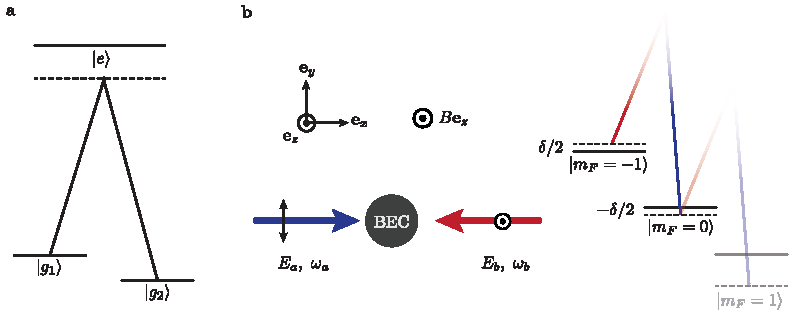
\includegraphics[]{Figures/Chapter3/Raman_coupling.pdf}
\caption[Raman coupling with two-photon transitions]{\note{TODO:write caption}}
\label{fig:Raman_coupling}
\end{center}
\end{figure*}

Consider two laser beams counter propagating along $\ex$ and with polarizations along $\ey$ and $\ez$ as is shown in Figure~\ref{fig:Raman_coupling}b. The electric field from the Raman beams is given by
%
\begin{equation}
  \mathbf{E}(x,t) = E_a\cos(k_a x-\omega_at)\e_y + E_b\cos(k_b x+\omega_bt)\ez,
\end{equation} 
%
and consequently 
%
\begin{equation}
	\mathbf{E}^*\times\mathbf{E} = 2i E_a E_b\cos(2\kl x-\Delta\omega t)\ex,
\end{equation}
%
where $\Delta\omega=\omega_a-\omega_b$. The geometry and wavelength of the Raman fields determine the natural units of the system: the single photon recoil momentum $k_{\mathrm{L}}=2\pi/\lambda_{\mathrm{R}}$ and its associated recoil energy $E_{\mathrm{L}}=\hbar^2k_{\mathrm{L}}^2/2m$, as well as the direction of the recoil momentum $\mathbf{k}_{\mathrm{L}}=k_{\mathrm{L}}\ex$. For most experiments we tune to the magic wavelength $\lambda_{\mathrm{R}}=790.032\,\nm$, so that the scalar light shift is zero and the scattering rate is minimized. We occasionally tuned away from this wavelength, for example when we were starving for laser power and wanted to increase our Raman coupling strength; Figure~\ref{fig:Raman_vs_lambda} shows the dependence of the Raman coupling strength and the lifetime on wavelength. 

\begin{figure*}[htb]
\begin{center}
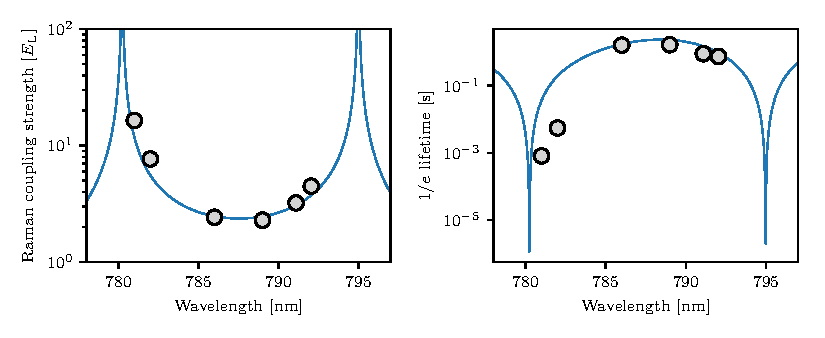
\includegraphics[]{Figures/Chapter3/Raman_vs_lambda.pdf}
\caption[Raman coupling strength and scattering rate as a function of wavelength]{Raman coupling strength and $1/e$ lifetime as a function of wavelength for a pair of Raman beams with waist $w_0\sim \unit[150]{\mu m}$ and powers of $~\unit[50, 10]{\mu W}$.}
\label{fig:Raman_vs_lambda}
\end{center}
\end{figure*}

The Raman Hamiltonian is given by
%
\begin{equation}
	\hat{H}_{R}=\Omega\cos(2\kl x-\Delta\omega t)\fx
\end{equation}
%
where $\Omega=\alpha^{(1)}g_F E_a E_b/g_J\propto \sqrt{I_a I_b}$ is the Raman coupling strength. In a frame rotating with angular frequency $\Delta\omega$ corresponding to applying the unitary transformation $\hat{U}(t)=\exp(-i\Delta\omega t\fz)$ and neglecting the fast terms rotating at frequency $2\Delta\omega$ (applying a RWA) the transformed Hamiltonian is
%
\begin{equation}
	\hat{U}^{\dagger}\hat{H}_R\hat{U} - i\hbar\hat{U}^{\dagger}\partial_t\hat{U}=\Delta\omega \fz+\frac{\Omega}{2}\cos(2\kl x)\fx-\frac{\Omega}{2}\sin(2\kl x)\fy,
	\label{eq:basic_Raman}
\end{equation}
%
which describes a helically precessing magnetic field with period $\lambda_{\rm R}/2$ which is illustrated in Figure~\ref{fig:B_eff}.

\begin{figure*}[htb]
\begin{center}
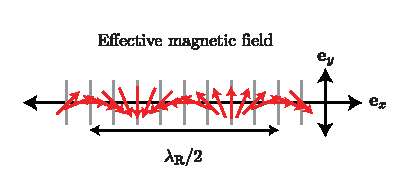
\includegraphics[]{Figures/Chapter3/B_eff.pdf}
\caption[Effective magnetic field from two cross polarized Raman laser beams]{The effective Raman Hamiltonian can be visualized as an interaction with an effective helically precessing magnetic field.}
\label{fig:B_eff}
\end{center}
\end{figure*}

\note{TODO: the two-level stuff maybe doesn't really make much sense anymore}


\subsection{Spin-orbit coupling}

The Raman Hamiltonian from Equation~\ref{eq:basic_Raman} can be massaged a bit more to make it look like a spin-orbit coupled\footnote{Not to be confused with the spin-orbit coupling giving rise to the fine and hyperfine structure mentioned earlier, perhaps a better name could be spin-momentum coupling} Hamiltonian that is familiar to condensed matter physicists. If we apply a spin-dependent momentum boost which is described by the unitary operator $\hat{U}(\kl)=\exp(i2\kl x \fz)$ the full Hamiltonian including the Raman coupling and the free 
%
\begin{equation}
 	\hat{H}_{\rm{SOC}} = \frac{\hbar^2}{2m}\left(\hat q_x-2\kl\fz\right)^2+\frac{\Omega}{2}\fx + \delta\fz + \hbar\epsilon\left(\mathds{1}-\frac{\fz^2}{\hbar^2}\right),
 \end{equation} 
%
where $\delta=E_-1-\Delta\omega$. We can go from an $F=1$ 3 system to an effective spin-$1/2$ system if we set $\Delta\omega=E_{-1}-E_0$ and consider a sizable quadratic Zeeman shift $\epsilon$, the $m_F=1$ state can be adiabatically eliminated. 
%
\begin{equation}
	\hat{H}_{SOC}=\frac{\hbar^2}{2m}(q_x-\kl\hat{\sigma}_y)^2+\frac{\hbar}{2}\Omega\hat{\sigma}_z + \frac{\hbar}{2}\delta\hat{\sigma}_y
\end{equation}
%
where $\sigma_{x,y,z}$ are the Pauli matrices. The Hamiltonian above corresponds to an equal superposition of Rashba-type~\cite{bychkov_oscillatory_1984} ($\propto \hat{\sigma}_xk_y-\hat{\sigma}_yk_x$) and Dresselhaus-type~\cite{dresselhaus_spin-orbit_1955} ($\propto -\sigma_xk_y-\sigma_y k_x$) SOC with an effective magnetic field $\propto\Omega$ in the $\ey-\ez$ plane~\cite{galitski_spin-orbit_2013,lin_spin-orbit-coupled_2011}. In Chapter~\ref{ch:Rashba} I discuss the Rashba term in more detail and introduce a way of engineering a system with only Rashba-type SOC using multiple internal levels and Raman transitions. 



\note{TODO: make plots of gamma, us and uv. Use data from atoms as an example?}

% In earlier sections we discussed the spin-orbit coupling interaction between spin and angular momentum that gives rise to the atomic level structure. In condensed matter systems, there is another kind of spin-orbit coupling that links the spin of the electrons with the linear or crystal momentum. In 2D materials, SOC can be represented as a sum of Rashba~\cite{bychkov_oscillatory_1984} and Dresselhaus~\cite{dresselhaus_spin-orbit_1955} SOC. 




\section{Floquet theory}



\section{Absorption imaging}
\subsection{Time of flight imaging}
Mention Stern Gerlach here
\subsection{Calibrating $I_{\rm{sat}}$}

%%%%%%%%%%%%%%%%%%%%%%%%%%%%%%%%%%%%%%%%%%%%%%%%%%%%%%%%%%%%%%%
%
%Graveyard
%
%%%%%%%%%%%%%%%%%%%%%%%%%%%%%%%%%%%%%%%%%%%%%%%%%%%%%%%%%%%%%

% The eigenstate of the perturbed Hamiltonian are linear combinations of the unperturbed eigenstates $\ket{n}$  
% %
% \begin{equation}
% 	\ket{\psi}=\sum_n a_n(t)e^{-iE_n t/\hbar}\ket{n},
% \end{equation}
% %
% using the time-dependent Schr\"odinger equation we can find equations for the coefficients $a_n(t)$
% %
% \begin{equation}
% 	i\hbar \partial_ta_n(t)=\sum_k\bra{n}\hat{H}_{\rm{dip}}\ket{k}a_k(t)e^{i\omega_{n,k}t}
% \end{equation}
% %
% where $\omega_{nk}=(E_n-E_k)/\hbar$. If we consider the perturbation being turned on at $t=0$ and if $\omega\neq\omega_{nk}$ the first order coefficient is
% %
% \begin{equation}
% 	a_n^{(1)}=-\frac{\bra{n}d_iE_0\ket{m}}{2\hbar}
% \end{equation}

% For $S$ electrons the hyperfine splitting can be described by the Hamiltonian $\hat H_{\rm{hfs}} = A_{\rm{hfs}}\mathbf{I}\cdot\mathbf{J}$\footnote{Notice how both the fine and hyperfine structure arise from a spin-orbit coupling interaction, we will discuss a very different type of spin-orbit coupling in future chapter.}. Figure~\ref{fig:fs_hfs}c shows the fine structure getting further split into states of total angular momentum $\mathbf{F}=\mathbf{J}+\mathbf{I}$. $\Rb87$ has a nuclear spin $I=3/2$ and therefore its ground state hyperfine configuration has $F=1$ and $F=2$. Here
% ~\cite{Steck} 

% Lets now consider the example of an atom in the presence of an oscillating electric field with amplitude $E_0$ and polarization $\epsilon$ $\mathbf{E}=E_0\cos(\omega t)\boldsymbol{\epsilon}$. We will use time-dependent perturbation theory to calculate the resulting energy shifts. 


% So far I have considered that the excited state has an infinitely long lifetime and does not decay. However, in reality the atom can spontaneously emit photons and decay. The lifetime of the excited state is given by $1/\Gamma_{e_j}$. The exponential decay of the excited state corresponds to adding a imaginary contribution to the energy $E_{e_j}\rightarrow E_{e_j}-i\hbar\Gamma_{e_j}/2$ which makes the polarizability a complex valued number. 

% The decay rate of a transition is related to the square of the dipole matrix element via Fermi's golden rule~\cite{Sakurai}

% \begin{equation}
% 	\Gamma_{J_gJ_e}=\frac{\omega_0^2}{3\pi\epsilon_0\hbar c^3}\frac{2J_g+1}{2J_e+1}\vert\langle g \| \mathbf{d}\|e\rangle\vert^2
% \end{equation}

% where $\vert\langle g \| \mathbf{d}\|e\rangle\vert^2$ is a reduced matrix element
% I will now look at the scalar polarizability term for Alkali atoms. For the case of far-detuned light such that the hyperfine $F$ levels are not well resolved the scalar polarizability can be calculated using the fine structure $J$ states. For an atom in an initial state $J$

% use scattering rate to find reduced matrix element write final expresion. skip the j, go back to generic notation
% %
% \begin{equation}
%  	\alpha^{(0)}\approx\sum_{J'}\frac{\vert\langle J \| \mathbf{d}\|J'\rangle \vert^2}{3\hbar}\left(\frac{1}{\omega+\omega_{JJ'}}-\frac{1}{\omega-\omega_{JJ'}}\right)
%  \end{equation} 
% If we consider Alkali atoms in the ground state hyperfine manifold in the presence of far detuned light such that the hyperfine levels are not well resolved we need to calculate the matrix elements using the $J$ states


% the scalar polarizability takes the form 
% The matrix element in Equation~\ref{eq:scalar_pol} can be expressed using the Wigner-Eckart theorem~\cite{Sakurai} in terms of the Clebsch-Gordan coefficients and the reduced matrix elements. 
%Here I will only consider the case of oscillating electric fields $\mathbf{E}=E_0\cos(\omega t)\boldsymbol{\epsilon}$ (i.e. plane waves of electromagnetic radiation) which are relevant to our experiments. 

% write tensor polarizability, write it into irreducible components. Mention that tensor component is very small and ignored. 

% Scalar polarizability: real part is light shift, complex part is scattering. Apply rwa and get the classic expressions for trapping potential and scattering. Make plot of polarizabily for RB87 Sub subsection: dipole traps

% Tensor polarizability



% Can break interaction into scalar, vector and tensor part. Interaction can also be resonant or off-resonant.

% \note{Why do you only get second order perturbation theory effects? I think it has something to do with unperturbed atomic states being eigenstates of the parity operator}

% We use light tuned to the magic wavelength $\lambda_{\mathrm{R}}=790.032\,\nm$ so that the scalar light shift vanishes (Section~\ref{sec:scalar_light_shift}). Because the light is considerably detuned from the D1 and D2 lines we do not take into account coupling into any of the excited states\footnote{Some atoms are inevitably excited of course, leading to heating from spontaneous emission (Equation~\ref{eq:scattering})}

% \note{Something about what we use this transitions for and how we usually ignore all other levels. (???)}

% \note{TODO: what about matrix elements between -1 and +1?. Move to intro chapter}


			% !TEX root = mainthesis.tex
%Chapter 4

\renewcommand{\thechapter}{4}

\chapter{Manipulation and detection of ultra-cold atoms}

\section{Atomic structure}

\section{Magnetic fields}
\subsection{Static magnetic fields}
Uniform fields: Zeeman splitting, Breit-Rabi formula
Gradients: Quadrupole potentials and Stern-Gerlach

\subsection{Oscillatory fields}
RF coupling and microwave coupling

\section{Electric fields: Atom-light interaction}

Can break interaction into scalar, vector and tensor part. Interaction can also be resonant or off-resonant.

\subsection{Scalar light shift: Dipole traps and optical lattices}

\subsection{Vector light shift: Raman coupling}

\section{Floquet}
How to treat systems when RWA is not valid and how to create new effective (stroboscopic) Hamiltonians.

\section{Absorption Imaging}
\subsection{Time of flight imaging}
\subsection{Partial transfer absorption imaging: magnetic field stabilization}



			% !TEX root = mainthesis.tex
%Chapter 5
\externaldocument{Chapter8.tex}

\renewcommand{\thechapter}{5}

\chapter{Fourier Transform Spectroscopy}
\label{ch:Fourier_spectroscopy}


The high level of control and tunability in ultracold atomic systems makes them an ideal platform for analog simulation of materials and other complex systems. The properties of these engineered `atomic' materials depend on the underlying single particle energies and it is therefore important to characterize them. Fourier transform spectroscopy was developed for this purpose. 

Many spectroscopy techniques in atomic physics rely on using 
a source of coherent electromagnetic radiation with a well known frequency that probes the internal structure of a system (atom). For example, in absorption spectroscopy~\cite{demtroder_doppler-limited_2008} coherent light is sent through an atomic medium and if the frequency of the light is resonant with an atomic transition it will be absorbed and a reduced transmission will be measured. Other variants of spectroscopy (e.g. Rabi spectroscopy~\cite{rabi_space_1937}, spin-injection spectroscopy~\cite{cheuk_spin-injection_2012}) work under a similar principle: atoms absorb and emit photons with frequencies equal to the transition energies between internal states. .

Fourier transform spectroscopy instead employs the connection between the energy spectrum of a system and its dynamics. This connection has been exploited to study the spectrum of both condensed matter \cite{jonas_two-dimensional_2003} and cold atom systems \cite{yoshimura_diabatic-ramping_2014,wang_atom-interferometric_2015} alike.
As opposed to other techniques, Fourier spectroscopy relies only on following the unitary evolution of an initial state suddenly subjected to a Hamiltonian of interest and measuring probabilities in a basis that does not diagonalize that Hamiltonian. 
% This spectroscopic tool is also useful for studying the energy spectrum of more complex time-dependent periodically driven systems \cite{eckardt_superfluid-insulator_2005,goldman_periodically_2014}, which are well suited for engineering and tuning Hamiltonians.

The frequency resolution of Fourier transform spectroscopy is limited only by the coherent evolution timescale of the system under study and can otherwise be applied to any system. Other applications of this technique implemented in our lab that are not included in this Chapter include measuring the dispersion relation of a Rashba spin-orbit coupled gas (see Chapter~\ref{ch:Rashba}) and the band structure of a sub-wavelength optical lattice~\cite{anderson_realization_2019}.

In this Chapter I first give a general description of the Fourier transform spectroscopy technique in Section~\ref{sec:fs-theory}. Then in Section~\ref{sec:fs-exp} I describe a set of experiments where we engineered a tunable spin-orbit coupled system and applied Fourier transform spectroscopy. This work was published in~\cite{valdes-curiel_fourier_2017}.

% which offers the advantage of simultaneous recording
% of a large spectral interval and with it a short measuring time.

\section{Operating principle of Fourier spectroscopy}
\label{sec:fs-theory}
%
\begin{figure*}[!ht]
	\begin{center}
		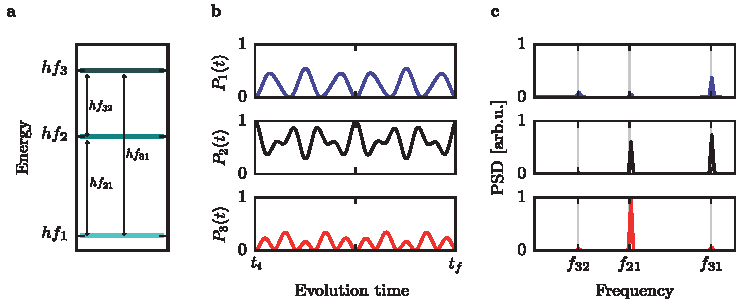
\includegraphics{Figures/Chapter5/Fig1.pdf}
		\caption[Operating principle of Fourier spectroscopy]
		{
			{\bf a.} Eigenenergies of a three-level system described by $\hat{H}'(\Omega_1,\Omega_2,\Omega_3)$. 
			{\bf b.} The system is prepared in $\ket{\psi_2}$ and subjected to $\hat{H}'$ at time $t_i$. The three panels show the occupation probabilities of the states $\ket{\psi_1}$ (blue), $\ket{\psi_2}$ (black), and $\ket{\psi_3}$ (red) in the measurement basis, for evolution times up to $t_f$. 
			{\bf c.} Power spectral density of the occupation probabilities from panel b. The three peaks in the Fourier spectra correspond to the energy differences present in panel a.
		\label{fig:Figure1}}
	\end{center}
\end{figure*}
%
We focus on a system where we can measure the occupation probabilities of a set of orthonormal states $\{\ket{\psi_i}\}$ that fully span the accessible Hilbert space of the system. We then consider the time evolution of an arbitrary initial state $\ket{\Psi_0}=\sum\limits_{i}a_i\ket{\psi_i}$ as governed by a Hamiltonian $\hat{H}'(\{\Omega_i \})$ and observe the occupation probabilities of the $\{\ket{\psi_i}\}$ states of the measurement basis as a function of time. When $\hat{H}'$ is applied, the evolution of the initial state is $\ket{\Psi(t)}=\sum\limits_{i,j}a_ic_{i,j}e^{-iE'_jt/\hbar}\ket{\psi'_j}$, where $E'_j$ and $\ket{\psi'_j}$ are the eigenenergies and eigenstates of $\hat{H}'$, and $c_{i,j}(t)=\braket{\psi_i}{\psi'_j}$. The probability 
%
\begin{align}
P_k(t)=&|\braket{\psi_k}{\Psi(t)}|^2=\lvert\sum\limits_{i,j}a_ic_{i,j}c^{*}_{j,k}e^{-iE'_jt/\hbar}\rvert^2
\label{Eq:Probability}
\end{align}
%
of finding the system in a state $\ket{\psi_k}$ of the measurement basis can be expressed as a sum of oscillatory components, with amplitude given by the magnitude of the overlap integrals between the initial state and the eigenvalues of $\hat{H}'$
\begin{align}
%P_k(t)=\tilde{a}_k+\sum\limits_{i\neq j}\tilde{b}_{i,j,k}\cos(2\pi f_{j,j'}t),
P_k(t)=1+\sum\limits_{i,j\neq l} 2\lvert a_i^2c_{i,j}c_{j,k}c_{i,l}c_{l,k}\rvert \cos(2\pi f_{j,l}t),
\end{align}
where $f_{j,l}=(E'_{j}-E'_{l})/h$ is the frequency associated with the energy difference of two eigenstates of the Hamiltonian.
Fourier spectroscopy relies on measuring the populations on each state of the measurement basis as a function of time, and extracting the different frequency components $f_{j,l}$ directly by computing the discrete Fourier transform. The bandwidth and frequency resolution of the measurement are determined by the total sampling time and the number of samples. For $N$ samples separated by a time interval $\Delta t$, the highest resolved frequency will be $f_{\mathrm{bw}}=1/2\Delta t$, with resolution $\Delta f=1/\Delta tN$. This resolution can be decreased if the Fourier transform is calculated using certain types of windowing functions that enhance signal to noise.  Any  higher frequency  $f>f_{\mathrm{bw}}$ will be aliased and measured in the Fourier spectrum as $f_{\mathrm{alias}}=\vert f - m/\Delta t \vert$, where $m$ is an integer. If interactions are present in the system, the dynamics get modified in a time scale given by the magnitude of the interactions, giving an additional constraint to the smallest frequency components of a single particle Hamiltonian that can be resolved with our technique.

Figure~\ref{fig:Figure1} illustrates the principle of Fourier spectroscopy for a three level system, initially prepared in the state $\ket{\Psi_0}=\ket{\psi_2}$, subject to the Hamiltonian
%
\begin{equation}
\hat{H}'=\begin{pmatrix}
E_1 & 0 & 0  \\
0 & E_2 & 0  \\
0 & 0 & E_3 \\
\end{pmatrix}
+\hbar\begin{pmatrix}
0 & \Omega_1 & \Omega_2  \\
\Omega_1^{*} & 0 & \Omega_3  \\
\Omega_2^{*} & \Omega_3^{*} & 0
\end{pmatrix},
\end{equation}
%
where we measure the occupation probability as a function of time for each of the $\{\ket{\psi_1}, \ket{\psi_2},\ket{\psi_3}\}$ states. The three eigenenergies $E'_i=hf_i$ that result from diagonalizing $\hat{H}'$are displayed in figure~\ref{fig:Figure1}a. The three energy differences $hf_{jj'}$ between the levels determine the oscillation frequencies of the occupation probabilities, as can be seen in figure~\ref{fig:Figure1}b. Finally, a plot of the power spectral densities (PSD) in figure~\ref{fig:Figure1}c shows three peaks at frequencies corresponding to the three relative energies of $\hat{H}'$. 
%
\section{Measuring the SOC dispersion with Fourier transform spectroscopy}
\label{sec:fs-exp}
%
\subsection{System}

We applied the Fourier transform spectroscopy technique to measure the dispersion relation of BECs with (tunable) SOC. All of our experiments started with BECs containing about $4\times 10^4$ atoms in the $\ket{f=1,m_F=-1}$ hyperfine state. The experiments described in Section~\ref{sec:application_of_fs} were performed in an optical dipole trap with frequencies $(\omega_x,\omega_y,\omega_z)/2\pi=(42(3),34(2),133(3))\Hz$. We later modified the trapping frequencies in the $xy$ plane to try to make them more symmetric for the experiments described in Section~\ref{sec:effective_mass}. We broke the degeneracy of the three $m_F$ magnetic sub-levels by applying a $1.9893(3)\,$mT bias field along $\mathbf{e}_z$ that produced a $\omega_Z / 2\pi  = 14.000(2) \MHz$ Zeeman splitting, and a quadratic Zeeman shift $\epsilon$ that shifted the energy of $\ket{f=1,m_F=0}$ by $-h\times 28.45\, \kHz$. We transfered atoms into the $\ket{f=1,m_F=0}$ state using ARP (see~\ref{sec:arp}) and then we monitored and stabilized the magnetic field using partial transfer absorption imaging as described in Chapter~\ref{sec:ptai} by applying a pair of $\unit[250]{\mu s}$ microwave pulses, each of them detuned by $\pm \unit[2]{kHz}$ from the $\ket{f=1, m_F=0}\leftrightarrow\ket{f=2, mf=1}$ transition.

\begin{figure*}[!ht]
	\begin{center}
		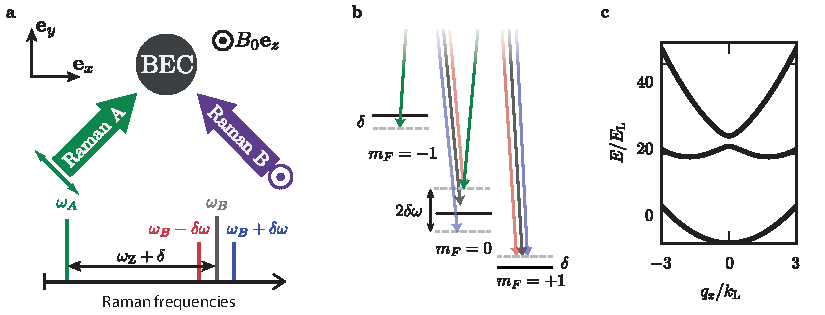
\includegraphics{Figures/Chapter5/Fig2.pdf}
		\caption[Experimental setup for engineering a tunable system with equal contributions of Rashba and Dresselhaus-type spin-orbit coupling]
		{
			{\bf a.} Setup. A bias magnetic field $B_0\ez$, with $B_0=1.9893$\,mT splits the hyperfine energy levels of the $f=1$ manifold of $^{87}$Rb by $\omega_Z/2\pi=14$\,MHz. A pair of cross polarized Raman beams propagating along $\ex+\ey$ and $\ex-\ey$ couple the atoms' momentum and spin states. 
			{\bf b.} The Raman frequencies are set to $\omega_A=\omega_L+\delta$ and $\omega_B=\omega_L+\omega_Z$. We add frequency sidebands to $\omega_B$, separated by $\pm \delta\omega$. The amplitude modulation from the interference between the multiple frequency components results in tunable SOC.
			{\bf c.} SOC dispersion for Raman coupling strength $\Omega_0=12E_{\mathrm{L}}$ and $\Omega=0$, on four photon resonance.
		\label{fig:Figure2}}
	\end{center}
\end{figure*}

We induced spin-orbit coupling using a pair of intersecting, cross polarized Raman laser beams propagating along $\mathbf{e}_x+\mathbf{e}_y$ and $\mathbf{e}_x-\mathbf{e}_y$, as shown in figure~\ref{fig:Figure2}a and b. This beams have angular frequency $\omega_A=\omega_L+\delta$ and $\omega_B=\omega_L+\omega_Z$, where $2\delta$ is the, experimentally controllable, detuning from four photon resonance between $m_F=-1$ and $m_F=+1$. 

Our system was well described by the Hamiltonian including atom-light interaction along with the kinetic contribution
 
 \begin{align}
 \begin{split}
 \hat{H}_{\mathrm{SOC}} = &\frac{\hbar^2q_x^2}{2m} + \alpha q_x\hat{F}_z  + 4E_{\mathrm{L}}\hat{\mathbb{1}} + \hbar\Omega_{\mathrm{R}}\hat{F}_x  +(4E_{\mathrm{L}}-\epsilon)(\hat{F}_z^2-\hat{\mathbb{1}}) +\hbar\delta\hat{F}_z,
 \label{Eq:SOCone}
 \end{split}
 \end{align}
 %
where $q$ is the quasimomentum, $\hat{F}_{x,y,z}$ are the spin-1 angular momentum matrices,  $\alpha=\hbar^2k_{\mathrm{L}}/m$ is the SOC strength, and $\Omega_{\mathrm{R}}$ is the Raman coupling strength, proportional to the Raman laser intensity. The Raman field coupled $\ket{m_F=0,\, q=q_x}$ to $\ket{m_F=\pm1,\, q=q_x\mp 2k_{\mathrm{L}}}$, generating a spin change of $\Delta m_F=\pm1$ and imparting a $\mp 2k_{\mathrm{L}}$ momentum. The eigenstates of $\hat{H}_{\mathrm{SOC}}$ are linear combinations of these states and $\ket{m_F=0,\,q=q_x}$, and the set $\{\ket{m_F,q}\}$ constituted the measurement basis for Fourier transform spectroscopy.

Figure \ref{fig:Figure2}c shows a typical band structure of our spin-1 SOC system as a function of quasimomentum for a large and negative quadratic Zeeman shift $-\epsilon>4E_{\mathrm{L}}$. In this parameter regime the ground state band has a nearly harmonic dispersion with an effective mass $m^{*} = \hbar^2[d^2E(k_x)/d^2x]^{-1}$, only slightly different from that of a free atom. 

\subsection{Tunable SOC}
We engineered a highly tunable dispersion relation in which we can independently control the size of the gap at $q_x=0$ as well as the SOC strength $\alpha$ by adding frequency sidebands to one of the Raman beams. The state of the system can change from $\ket{m_F=-1,\,q=q_x+2k_{\rm{L}}}$ to  $\ket{m_F=1,\,q=q_x-2k_{\mathrm{L}}}$ by absorbing a red detuned photon first followed by a blue detuned photon and vice versa, in a similar way to the M\o lmer-S\o rensen entangling gate in trapped ion systems \cite{sorensen_entanglement_2000}. When we set the angular frequencies of the sidebands to $\omega=\omega_{\mathrm{A}}+\omega_Z \pm \delta\omega$, the Hamiltonian (Equation~\ref{Eq:SOCone}) acquired a time-dependent coupling $\Omega_{\mathrm{R}}(t)=\Omega_0 + \Omega\cos(\delta\omega t)$. This periodically driven system is well described by Floquet theory \cite{floquet_sur_1883} (see Chapter~\ref{sec:Floquet_theory}). Figure~\ref{fig:Floquet} shows the spectrum of Floquet quasi-energies for a system described by~\ref{Eq:SOCone} where $\Omega_{\rm R}$ oscillates with angular frequency $\delta\omega$. 
%
\begin{figure*}[htb]
	\begin{center}
		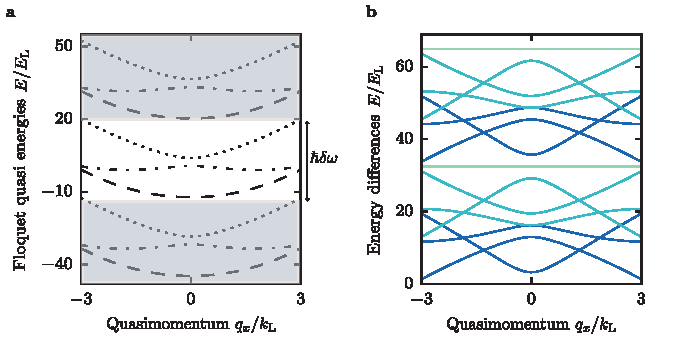
\includegraphics{Figures/Chapter5/Fig3.pdf}
		\caption[Floquet quasi-energy spectrum of a three-level system with spin-orbit coupling and periodic coupling strength]
		{
			{\bf a.} Floquet quasi-energies of a three level Hamiltonian with SOC and time periodic coupling strength. The quasi-energies are grouped into manifolds consisting of three levels that get repeated with a periodicity equal to $\hbar\delta\omega$.
%
			{\bf b.} Energy differences of the Floquet quasi-energies. Each color represents the energy difference, separated by a fixed number of neighboring levels. When the number of neighboring levels is a multiple of 3, the energy differences are straight lines, a result of the periodic structure of the Floquet manifolds. 
		\label{fig:Floquet}}
	\end{center}
\end{figure*}

We found an effective time-independent Hamiltonian using a unitary transformation $\hat{U}(t)$ and applying a RWA. Recall that the time evolution of a wave function in a transformed frame  $\ket{\psi'}=\hat{U}^{\dag}\ket{\psi}$ is given by the time dependent Schr\"odinger equation with a Hamiltonian $\hat{H}'=\hat{U}^{\dag}\hat{H}\hat{U}-i\hbar\hat{U}^{\dag}\partial_t\hat{U}$. Here we used 
\begin{equation}
\hat{U}(t)=\mathrm{exp}[-i\frac{\Omega}{\delta\omega}\sin(\delta\omega t)\hat{F}_x]
\end{equation}
%
so that $i\hbar\hat{U}^{\dag}\partial_t\hat{U}=\hbar\Omega_{\rm R}(t)\fx$. The transformed Hamiltonian $\hat{H}'(t)$ has terms proportional to $\sin(\Omega/\delta\omega\sin(\delta\omega t))$, $\sin^2(\Omega/\delta\omega\sin(\delta\omega t))$, $\cos(\Omega/\delta\omega\sin(\delta\omega t))$ and $\cos^2(\Omega/\delta\omega\sin(\delta\omega t))$ which we simplified using the Jacobi-Anger expansion for large values of $\theta$
\begin{align*}
&\cos(z\sin\theta)= J_0(z) + 2\sum_{n=1}^{\infty}J_{2n}(z)\cos(2n\theta) \approx J_0(z) \\
&\sin(z\sin\theta)= 2\sum_{n=0}^{\infty}J_{2n+1}(z)\sin((2n+1)\theta) \approx 0,
\end{align*} 
%
 where $J_n$ is the the $n$th order Bessel function of the first kind.

This approximation is valid for $\hbar\delta\omega > \vert\epsilon\vert+12E_{\rm{L}}$ and $\vert q_x\vert \leq 2\kl$ so that quasi-energy manifolds are well separated as in figure~\ref{fig:Floquet}a. The resulting Hamiltonian retained the form of Equation~\ref{Eq:SOCone} with renormalized coefficients and an additional coupling term:

\begin{align}
\begin{split}
\hat{H}_{Fl} = &\hat{H}_{SOC}(q,\Omega_0,\tilde{\alpha},\tilde{\delta},\tilde{\epsilon}) + \tilde{\Omega}\hat{F}_{xz},
\label{Eq:SOCeff}
\end{split}
\end{align}

where $\tilde{\alpha}= J_0(\Omega/\delta\omega)\alpha$, $\tilde{\Omega}=1/4(\epsilon+4E_{\mathrm{L}}) [J_0(2\Omega/\delta\omega)-1]$, $\tilde{\delta}=J_0(\Omega/\delta\omega)\delta$, and $\tilde{\epsilon}= 1/4(4E_{\mathrm{L}}-\epsilon) -
1/4(4E_{\mathrm{L}} + 3 \epsilon) J_0( 2\Omega/\delta\omega)$. $\hat{F}_{xz}$ is the $\hat{\lambda}_4$ Gell-Mann matrix that directly couples $\ket{m_F=-1, q=q_x+2k_{\mathrm{L}}}$ and $\ket{m_F=+1, q=q_x-2k_{\mathrm{L}}}$ states. The experimentally tunable parameters $\delta\omega$, $\Omega$ and $\Omega_0$ can be used to tune the SOC dispersion.

\subsection{Application of Fourier spectroscopy}
\label{sec:application_of_fs}

We used Fourier transform spectroscopy to measure the spectrum of the SOC Hamiltonian (Equation~\ref{Eq:SOCeff}) for three coupling regimes: (i) $\Omega_0\neq0$ and $\Omega=0$, (ii)  $\Omega_0=0$ and $\Omega\neq0$ and (iii) $\Omega_0\neq0$ and $\Omega\neq0$. We turned on the Raman laser non-adiabatically, in approximately $1	\,\mu\mathrm{s}$. We let the system evolve subject to $\hat{H}_{\mathrm{SOC}}$ for up to $900\, \mathrm{\mu s}$, and  then turned off the laser while releasing the atoms from the optical dipole trap. As usual, we resolved the spin and momentum distribution using Stern-Gerlach and a $\unit[21]{\ms}$ TOF which allowed us to measure the fraction of atoms in each state of the measurement basis $\{\ket{m_F, q}\}$. The density of sampling points and the maximum evolution time were chosen so that the bandwidth of the Fourier transform was comparable to, or larger than, the highest frequency in the evolution of the system while maximizing resolution. Experimental decoherence resulting in loss of contrast of the oscillations, which arises from magnetic field noise and small magnetic field gradients present in our apparatus, was an additional constraint that becomes significant around 1 ms. 

In order to map the full spin and momentum dependent band structure of $\hat{H}_{\mathrm{SOC}}$, we measured the time dependent occupation probabilities at a fixed Raman coupling strength and different values of Raman detuning $\delta$, for the same initial state $\ket{m_F=0, q_x=0}$. This detuning corresponded to the Doppler shift experienced by atoms moving relative to a light source with quasimomentum $q_x/k_{\mathrm{L}}=\hbar\delta/4E_{\mathrm{L}}$. We controlled the frequency and the detuning of the Raman beams using two AOMs, one of which is driven by up to three phase coherent frequencies (the carrier frequency plus two sidebands). For each of the three coupling cases that we measured, we applied the Raman beams at detuning values within the interval $\pm 12 E_{\mathrm{L}}$ which corresponds to quasimomentum values $\pm 3k_{\mathrm{L}}$.

This approach of changing detuning rather than using atoms with non-zero quasimomentum had the advantage that the state preparation was very reliable (making BECs at rest is easy\footnote{Well, nothing in the lab is really `easy'...}!) and we got very good signal to noise ratios due to the relatively high densities of the BECs. The downside is that if one is interested in looking at a large range of quasimomentum values, it takes a long time to repeat each experiment for different detuning values. In future experiments where we used Fourier transform spectroscopy we sacrificed some signal to noise for speed and used the momentum distribution of non-condensed atoms to parallelize our measurements. 

% For $\hat{H}_{\mathrm{SOC}}$, momentum and detuning are equivalent up to a numerical factor, $\delta/E_{\mathrm{L}}=4q_x/k_{\mathrm{L}}$, since the detuning term $\delta\hat{F}_z$ and the momentum term $\alpha\hat{q}_x\hat{F}_z$ have the same effect in the relative energies. This relation follows from the Doppler shift of the light frequency experienced by atoms moving relative to a light source: a stationary BEC in the laboratory reference frame dressed by a detuned laser field is equivalent to a moving BEC and a resonant laser field.

\subsection{Effective mass}
\label{sec:effective_mass}

Fourier transform spectroscopy only gives access to the relative energies of a Hamiltonian. If we want to recover the absolute energies we need to have an additional energy reference. For this particular set of experiments we had a ground state with a nearly quadratic dispersion and we could measure its effective mass which allowed us to obtain such reference. 

We measured the effective mass of the Raman dressed atoms by adiabatically preparing the BEC in the lowest eigenstate and inducing dipole oscillations. The effective mass of the dressed atoms  is related to the bare mass $m$ and the bare and dressed trapping frequencies $\omega$ and $\omega^{*}$ by the ratio $m^{*}/m=(\omega/\omega^{*})^2$. We measured this ratio following~\cite{lin_synthetic_2011}; we start in  $\ket{m_F=0,\, k_x=0}$ state and adiabatically turn on the Raman laser in $10\,\mathrm{ms}$ while also ramping the detuning to $\delta\approx0.5\,\El$, shifting the minima in the ground state energy away from zero quasi-momentum. We then suddenly bring the field back to resonance, exciting the BEC's dipole mode in the optical dipole trap. We measured the bare state frequency by using the Raman beams to initially induce motion but subsequently turn them off in $1\ms$ and let the BEC oscillate. For this set of measurements, we adjusted our optical dipole trap to give new trapping frequencies $(\omega_x, \omega_y, \omega_z)/2\pi=(35.6(4), 32.2(3), 133(3))\,\Hz$, nominally symmetric in the plane defined by $\ex$ and $\ey$. The Raman beams were co-propagating with the optical dipole trap beams; therefore, the primary axes of the dipole trap frequencies are at a $45^{\circ}$ angle with respect to the direction of $\mathbf{k}_{\mathrm{L}}$. 

The kinetic and potential terms in the Hamiltonian including the contribution of the Raman and optical dipole trap were

\begin{align}
\hat{H}_{\perp}= &\frac{\hbar^2q_x^2}{2m^{*}} + \frac{\hbar^2q_y^2}{2m}+\frac{m}{2}[\omega_{x'}^2x'^2+\omega_y'^2y'^2] \nonumber \\
= & \frac{\hbar^2}{2m^{\star}}k_x^2 + \frac{1}{2m}k_y^2+\frac{m}{4}[(\omega_{x'}^2+\omega_{y'}^2)(x^2+y^2)+2xy(\omega_{x'}^2-\omega_{y'}^2)],
\end{align}
%
where we have used  $x'=(x+y)/\sqrt{2}$ and   $y'=(x-y)/\sqrt{2}$ to rotate the dipole trap coordinates by $45^{\circ}$ . For an axially symmetric trap with $\omega_{x'}=\omega_{y'}$, the frequency of oscillation along the Raman recoil direction  is 

\begin{equation}
\omega_x^2=\frac{m}{2m^{*}}(\omega_{x'}^2+\omega_{y'}^2).
\label{Eq:meff}
\end{equation}

Our trap had a small $3.4$\,Hz asymmetry and therefore there is some coupling of the motion along the axis perpendicular to $\k_{\rm L}$ which becomes more significant at larger values of effective mass. The sampling times for the measurements were small compared to the trap asymmetry and therefore we can locally approximate the motion of the atoms by simple harmonic function with a frequency along $\ex$ given by Equation~\ref{Eq:meff}.

Figure~\ref{fig:Figure4} shows the dipole oscillations along the $\mathbf{e}_{x}$ and $\mathbf{e}_{y}$ directions for the three different coupling regimes we explored, as well as the bare state motion. The resulting mass ratios for the three coupling regimes are $m/m^{*}=$  (i) $1.04(8)$, (ii) $0.71(7)$, and (iii) $0.62(4)$.
\begin{figure*}[!ht]
	\begin{center}
		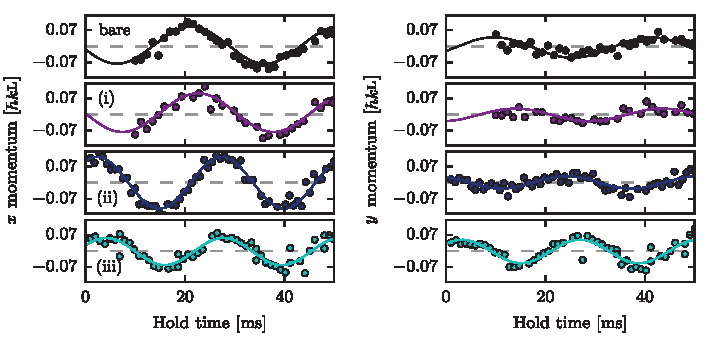
\includegraphics{Figures/Chapter5/Fig4.pdf}
		\caption[Dipole oscillations of a spin-orbit coupled BEC in a dipole trap]
		{  Oscillation of the BEC in the dipole trap along the  recoil directions $\mathbf{e}_{x}$ and  $\mathbf{e}_{y}$ for (top) bare atoms, and the three parameter regimes that we explored (i), (ii), and (iii).  We believe that the observed low amplitude oscillations along $\ey$ are due to the initial detuning ramp not being fully adiabatic. 
		\label{fig:Figure4}}
	\end{center}
\end{figure*}
%
\subsection{Measured dispersion}
\begin{figure*}[htb]
	\begin{center}
		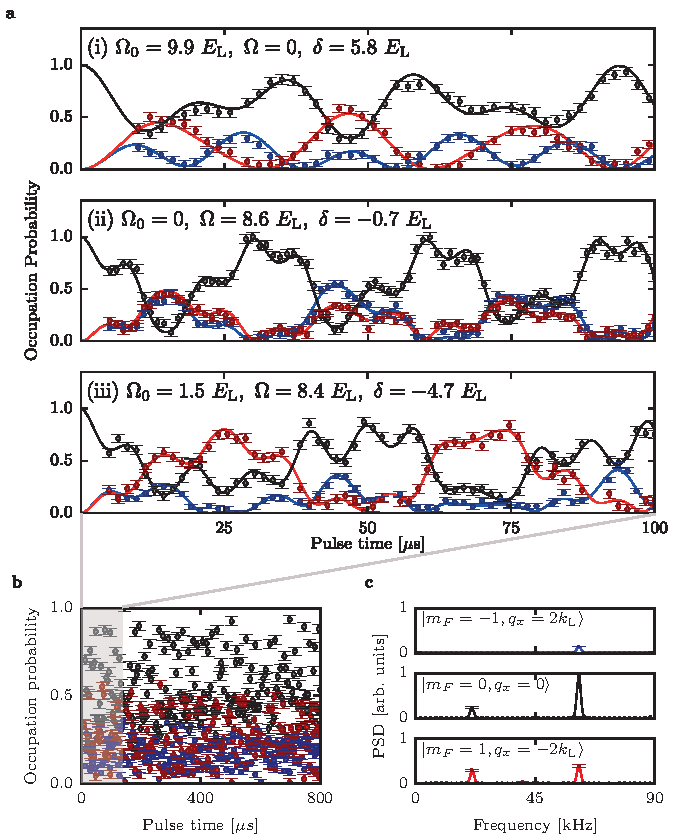
\includegraphics{Figures/Chapter5/Fig5.pdf}
		\caption[Time evolution and Fourier transforms of a SOC system]
		{{\bf a.}
		Occupation probability for the three states in the measurement basis $\ket{m_F=-1, q=q_x+2\kl}$ (blue), $\ket{m_F=0,q=q_x}$ (black), and $\ket{m_F=+1,q=q_x-2\kl}$(red),  following unitary evolution under $\hat{H}_{\mathrm{SOC}}$ for times up to 100 $\mu s$ at different spin-orbit coupling regimes: (i) $\Omega_0=9.9 E_{\mathrm{L}}$, $\Omega=04$,  $\delta=5.8 E_{\mathrm{L}}$, (ii) $\Omega_0=0$, $\Omega=8.6\,E_{\mathrm{L}}$,  $\delta=-0.7\,E_{\mathrm{L}}$, $\delta\omega=\epsilon+12\,E_{\mathrm{L}}$, and (iii) $\Omega_0=1.5\,E_{\mathrm{L}}$, $\Omega=8.4\, E_{\mathrm{L}}$,  $\delta=-4.7\,E_{\mathrm{L}}$, $\delta\omega=\epsilon+17\,E_{\mathrm{L}}$.
		{\bf b.} Occupation probability for long pulsing up to 800 $\mu$s for parameters as in (iii). 
		{\bf c.} Power spectral density of the occupation probability. We subtract the mean value of each probability before taking the Fourier transform to remove peaks at $f=0$. The peaks in the PSD then correspond to the relative eigenenergies of $\hat{H}_{SOC}$.
		}
		\label{fig:Figure5}
	\end{center}
\end{figure*}
%
We mapped the band structure of SOC atoms for three different coupling regimes. Figure~\ref{fig:Figure5}a shows representative traces of the measured occupation probabilities for short evolution times along with fits to the unitary evolution given by $\hat{H}_{\mathrm{SOC}}$ with $\delta$, $\Omega_0$, and $\Omega$ as free parameters. The fit parameters agree well with independent microwave and Raman power calibrations. In the lower two panels, where the Raman coupling strength was periodically modulated, the occupation probabilities oscillate with more than three frequencies since the full description of the system was given by a Floquet quasi-energy spectrum. Figure~\ref{fig:Figure5}b,c shows the occupation probabilities for the parameter regime (iii) for longer evolution times along with the PSD of the occupation probability of each spin state. 



\begin{figure}[!ht]
	\begin{center}
		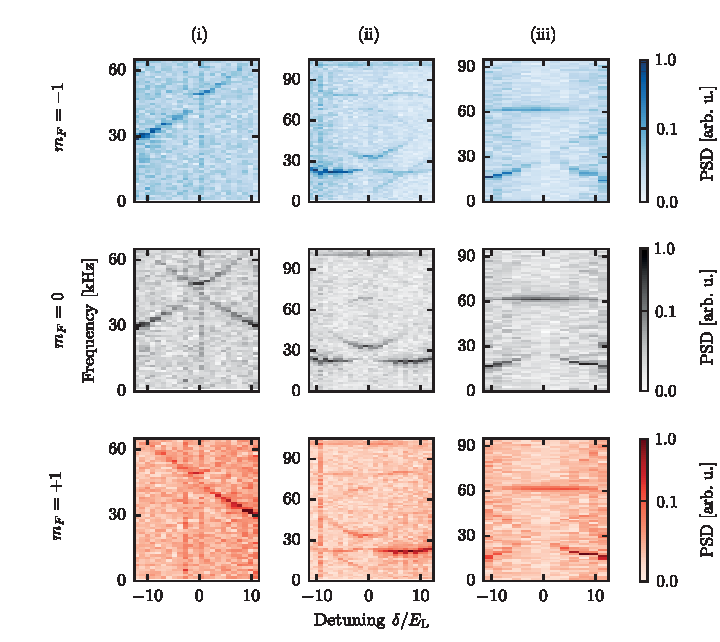
\includegraphics{Figures/Chapter5/Fig6a.pdf}
		\caption[Power spectral density of the time dependent occupation probability for each state in the measurement basis for three coupling regimes]
		{
			 Power spectral density of the time dependent occupation probability for each state in the measurement basis for three coupling regimes:
			{ (Left)} $\Omega_0=9.9 E_{\mathrm{L}}$, $\Omega=0$,
			{ (Center)} $\Omega_0=0$, $\Omega=8.6 E_{\mathrm{L}}$,  $\delta\omega=\epsilon+12 E_{\mathrm{L}}$, and
			{ (Right)} $\Omega_0=4.9 E_{\mathrm{L}}$, $\Omega=8.4 E_{\mathrm{L}}$,  $\delta\omega=\epsilon+17 E_{\mathrm{L}}$. Each panel is normalized to peak amplitude to highlight small amplitude features in the PSD of the periodically driven SOC, and the highest value on the frequency axis corresponds to the FFT bandwidth..
			{\bf b.} Spin-dependent SOC dispersion for three different coupling regimes. We combine the PSD of the occupation probability of the states $\ket{m_F=\pm 1, q_x=\mp 2k_{\mathrm{L}}}$, and shift each frequency by an amount proportional to the squared quasimomentum and the effective mass. The dashed lines are the calculated Floquet energies for the Hamiltonian using our calibration parameters. 
		}
		\label{fig:Figure6a}
	\end{center}
\end{figure}

We used a non-uniform fast Fourier transform algorithm (NUFFT) on a square window to obtain the power spectral density of the occupation probabilities since our data points were not always evenly spaced because of imperfect imaging shots. The heights of the peaks in the PSD are related to the magnitude of the overlap integrals between the initial state and the Raman dressed states. Figure~\ref{fig:Figure5}c shows the raw PSD of the time evolution of the system under $\hat{H}_{\mathrm{SOC}}$ for a given Raman coupling strength and detuning. We put together all the PSDs for the three coupling regimes in the spectra shown on the top three panels in figure~\ref{fig:Figure6a}. Each column corresponds to a different coupling regime and the colors represent the different spin states of the measurement basis. The spectra show that some overlap integrals vanish near $\delta=0$, which is manifested as missing peaks in the PSD. The periodic structure of the Floquet quasi-energy spectrum gives rise to peaks at constant frequencies of $\delta\omega$ and $2\delta\omega$ independently of the Raman detuning, and a structure that is symmetric about the frequencies $2\pi f_1=\delta\omega/2$ and $2\pi f_2=\delta\omega$. If you are interested in seeing another nice experiment where the Floquet quasienergy spectrum becomes important due to breaking of the RWA see~\cite{deng_observation_2015}.

\begin{figure}[!ht]
	\begin{center}
		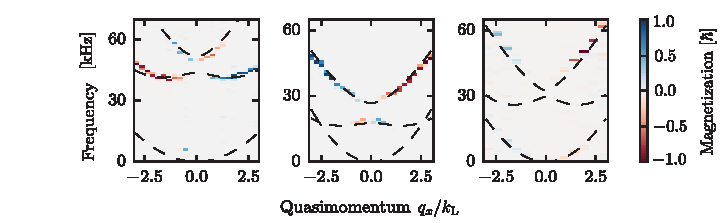
\includegraphics{Figures/Chapter5/Fig6b.pdf}
		\caption[Spin-dependent SOC dispersion for three different coupling regimes]
		{
			Spin-dependent SOC dispersion for three different coupling regimes. We combine the PSD of the occupation probability of the states $\ket{m_F=\pm 1, q_x=\mp 2k_{\mathrm{L}}}$, and shift each frequency by an amount proportional to the squared quasimomentum and the effective mass. The dashed lines are the calculated Floquet energies for the Hamiltonian using our calibration parameters. 
		}
		\label{fig:Figure6b}
	\end{center}
\end{figure}

We obtained the characteristic dispersion of a SOC system after adding a quadratic term to the PSD, proportional to the measured effective mass,  and after rescaling the detuning into recoil momentum units. We combined the PSD of the time evolution of the three $\ket{m_F}$ states to look at the spin dependence of the spectra. Figure \ref{fig:Figure6b} shows the measured dispersion relations as well as the Floquet quasi-energies calculated for the Hamiltonian parameters obtained from our calibrations. The spectral lines that can be resolved with our technique depend on the overlap integrals of the initial state with the target Hamiltonian eigenstates. Additional energies can be measured by repeating the experiment with different initial states. The spectral lines we were able to resolve are in good agreement with the calculated energies of the Hamiltonian. 

\begin{figure*}[!ht]
	\begin{center}
		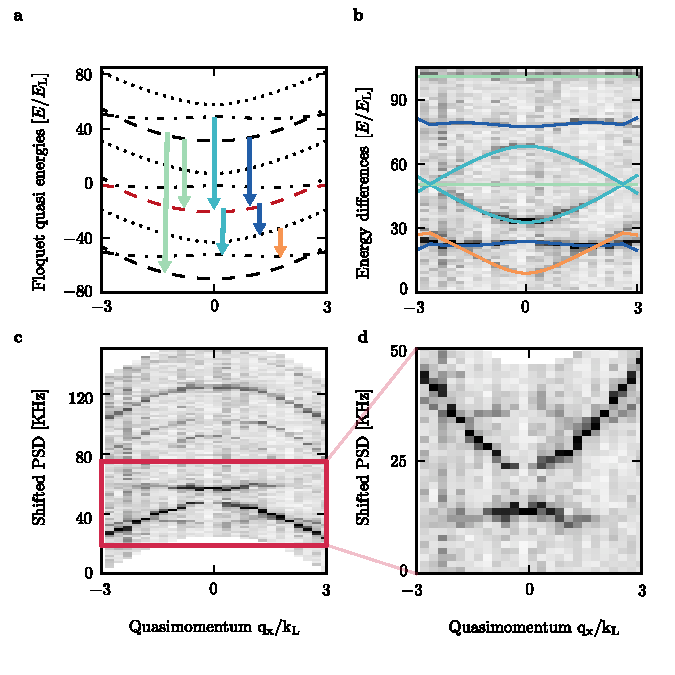
\includegraphics{Figures/Chapter5/Fig7.pdf}
		\caption[Converting energy differences into absolute energies]
		{  {\bf a} Floquet quasi-energy spectrum of a SOC Hamiltonian with periodic coupling strength. The red line represents the eigenstate that has the largest overlap with the initial $\ket{m_F=0}$ state. The arrows indicate the energies of the states that have non-zero overlap with the initial state and can be measured with Fourier transform spectroscopy.
		{\bf b} PSD of the occupation probability and numerically calculated energy differences between the levels indicated by the arrows on panel a.
		{\bf c} PSD shifted by a quadratic term $-\hbar^2 q^2_x/2m^*$. The red box indicates the region of interest where we can recover the SOC spectrum.
		{\bf d} We invert the frequency axis and shift it by $\delta\omega$.   
		}
		\label{fig:Figure7}
	\end{center}
\end{figure*}

Finally, because it is not so trivial to visualize what we did to recover the dispersion for the periodically driven SOC cases, Figure \ref{fig:Figure7} illustrates in detail the steps that were taken. The red line in panel a represents a level within a Floquet manifold that has the largest overlap integral with the initial $\ket{m_F=0, q=0}$ state. The peaks in the PSD correspond to energy differences between the marked level and the levels in neighboring Floquet manifolds pointed by the colored arrows. We show the theoretically computed energy differences on top of the measured PSD in panel b. The lowest frequency dominant peaks of the PSD correspond to energy differences with the adjacent lower Floquet manifold. To properly recover the SOC dispersion we shifted the PSD by a negative quadratic term $-\hbar^2q_x^2/2m^{*}$ as we show on panel c. We finally invert the frequency axis and shift it by $\delta\omega$. Including the effective mass to reconstruct the spectrum of the time-independent SOC case, amounts to shifting the PSD by a positive quadratic term.

\section*{Conclusion}

This chapter introduced the basic principles of the Fourier transform spectroscopy technique and used it to measure the spin and momentum dependent dispersion relation of a spin-1 spin-orbit coupled BEC. We additionally studied a periodically driven SOC system and found a rich Floquet quasi-energy spectrum. Our method can be applied generically to any system with long enough coherent evolution to resolve the energy scales of interest, and could prove particularly useful to study systems where it is harder to predict or compute the exact energies, such as cold atom realizations of disordered or highly correlated systems \cite{eisert_quantum_2015}. In our lab, this technique has been used to study the spectrum of a Rashba spin-orbit coupled system~\cite{valdes-curiel_unconventional_2019} and of a fractional period adiabatic superlattice~\cite{anderson_realization_2019}.

Our main interest in this project was originally to create tunable spin-orbit coupling and Fourier spectroscopy was conceived as a tool to characterize it. We realized that the use of Raman transitions from multiple frequency beams was equivalent to another experiment that achieved tunable SOC using amplitude modulated Raman coupling~\cite{jimenez-garcia_tunable_2015}.  %We therefore decided to focus on Fourier spectroscopy instead, a decision that turned out to be very fruitful for our lab as we continue to use this technique to characterize the spectrum of a variety of systems. 

% The idea of Fourier transform spectroscopy was born from a very different natured project. The project was originally conceived as a way to engineer tunable spin-orbit coupling using multiple-tone Raman transitions. The inspiration came from a previous project where we used multiple-tone Raman transitions to engineer a spin-1 spin-orbit coupled system whose ground state presented different magnetic phases~\cite{campbell_magnetic_2016}. Fourier spectroscopy was conceived as a new way to characterize the tunable dispersion relation resulting from our proposed coupling scheme. Unfortunately, we realized that this proposal was equivalent to another experiment that achieved tunable SOC using amplitude modulated Raman coupling~\cite{jimenez-garcia_tunable_2015}. We therefore decided to focus on studying Fourier spectroscopy instead, a decision that turned out to be very fruitful for our lab as we continue to use this technique to characterize the spectrum of a variety of systems. 








			% !TEX root = mainthesis.tex
%Chapter 6

% Our system is not the only one suffering from this issues; decoherence of quantum systems due to uncontrolled fluctuations of the environment presents fundamental obstacles in quantum science.
\newcommand{\reffig}[1]{Figure~\ref{#1}}
\newcommand{\refeq}[1]{Equation~\ref{#1}}
\externaldocument{Chapter4.tex}

\renewcommand{\thechapter}{6}

\chapter{Synthetic clock transitions through continuous dynamical decoupling}
\label{ch:clock_states}

Most of the experiments techniques described so far have used the hyperfine $\ket{m_F}$ states as effective spins and dressed them with an RF or Raman field. However, due to the linear dependence of their energies with respect to magnetic field, and our lack of control of environmental changes we always had to take special care to stabilize the magnetic field in the lab (see Section~\ref{sec:ptai}). An alternative to doing active magnetic field stabilization is to use clock transitions which are first-order insensitive to changes in magnetic field but unfortunately they are not present in all systems or for arbitrary system parameters. However, under almost all circumstances, clock transitions can be synthesized using dynamical decoupling protocols. These protocols involve driving the system with an external oscillatory field, resulting in a dynamically protected `dressed' system.

The idea of implementing continuous dynamical decoupling (CDD) in the lab came from a theoretical proposal to engineer Rashba type SOC using Raman beams and a strong RF field~\cite{campbell_rashba_2016}, the second being a necessary ingredient for CDD. We initially worked in implementing CDD protocols to create `synthetic clock states' as an intermediate step towards our final goal of engineering Rashba SOC. Just like with Fourier spectroscopy, CDD became a workhorse of the lab both for the stability it provides against environmental fluctuations and because it has given us access to non-zero matrix coupling elements that we otherwise would not have when working with the bare $\ket{m_F}$ states. We have continued to use CDD  not only for engineering Rashba SOC (Chapter~\ref{ch:Rashba}) but also to engineer subwavelength optical lattices\cite{anderson_realization_2019} and Hofstadter~\cite{hofstadter_energy_1976} cylinders (work in preparation). On the theory side, we developed a proposal that uses them as a platform for emulating $\mathcal{PT}$ symmetric Hamiltonians~\cite{trypogeorgos_perpetual_2018}. 

This Chapter discusses the implementation of CDD in the ground $F=1$ hyperfine manifold of ultracold $\Rb87$. First I give a general overview of dynamical decoupling and continuous dynamical decoupling. Then I describe the technical details and characterization of our CDD protocol which produces a protected three-level system of dressed-states and whose Hamiltonian is fully controllable. Finally, I discuss an implementation of concatenated CDD that renders the system first-order insensitive to both magnetic field noise and noise in the control field. This work was published in~\cite{trypogeorgos_synthetic_2018} and was done in parallel with~\cite{anderson_continuously_2018}.

\section{Basic principles of CDD}

Dynamical decoupling (DD) protocols consist in applying an external control Hamiltonian, generally implemented by a series of pulses, which has the effect of canceling out the dynamics that arise from ta quantum system coupling to the environment. DD was first introduced in the context of nuclear magnetic resonance (NMR) with the discovery of spin-echoes~\cite{hahn_spin_1950}, where a single `refocusing' pulse was applied to eliminate dephasing of spins resulting from variations in magnetic field. These ideas were later generalized in~\cite{viola_dynamical_1998} to protect a system from decoherence induced by interactions with a quantum environment. Continuous dynamical decoupling (CDD) relies on the application of time-periodic continuous control fields, rather than a series of pulses. %Unlike conventional dynamical decoupling protocols, CDD does not require any encoding overhead.% or quantum feedback measurements. 

A number of dynamical decoupling protocols, pulsed or continuous, have been shown to isolate quantum systems from low-frequency environmental noise~\cite{cohen_continuous_2017,fanchini_continuously_2007,aharon_fully_2016,biercuk_optimized_2009,cai_robust_2012,bermudez_robust_2012,baumgart_ultrasensitive_2016,kazakov_magic_2015,sarkany_controlling_2014}. Thus far, CDD has inoculated multi-level systems in nitrogen vacancy centers in diamond, nuclear magnetic resonance experiments, and trapped atomic ions~\cite{laucht_dressed_2017,farfurnik_experimental_2017,noguchi_generation_2012,golter_protecting_2014,timoney_quantum_2011,webster_simple_2013,barfuss_strong_2015,rohr_synchronizing_2014}, from spatiotemporal magnetic field fluctuations. 

\section{CDD of a spin-1 system}
\begin{figure}[!!h]
    \centering
    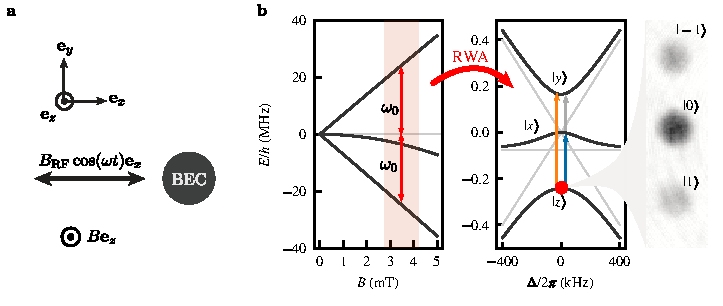
\includegraphics[]{Figures/Chapter6/fig1a.pdf}
    \caption[Implementing CCD.]{{\bf a.} Setup for implementing CCD using a strong RF magnetic field. {\bf b.}  Left: dependence of the $5^2S_{1/2}$, $F=1$ ground state of $\Rb87$ on magnetic field, where the quadratic dependence of the $\ket{m_F=0}$ state's Zeeman shift has been exaggerated so it is visible on the same scale.
    Center: energies of the $\xyz$ eigenstates, for $\Omega/2\pi=\SI{200}{kHz}$ (black curves) and $\Omega=0$ (grey curves).
    Right: TOF absorption image of $\ket{z}$ at $\Delta=0$, showing the constituent $\ket{m_F}$ states.
    }
    \label{fig:1}
\end{figure}

We implemented CDD using a strong RF magnetic field with strength $\Omega$ which linked the three $\ket{m_F}$ states comprising the $F=1$ electronic ground state manifold of $\Rb87$.
The RF field was linearly polarized along ${\bf e}_x$, and had angular frequency $\omega$ close to the Larmor frequency $\omega_0 = g_F \mu_{\rm B} B_0$ from a magnetic field $B_0 {\bf e}_z$; $g_F$ is the Lande $g$-factor and $\mu_{\rm B}$ is the Bohr magneton. Using the rotating frame approximation for the frame rotating at $\omega$ (which is valid for $\omega >>\Omega$), the system is described by
%
\begin{equation}
    \hat{H} = \hbar\Delta\fz+\hbar\epsilon(\fz^2-\hat{\mathbb{1}})+ \hbar\Omega \fx,
    \label{eq:h0}
\end{equation}
with detuning $\Delta=\omega-\omega_0$, quadratic Zeeman shift $\epsilon$, spin-1 angular momentum operators $\hat F_{x,y,z}$, and the identity operator $\hat{\mathbb 1}$.% For a detailed derivation of Equation~\ref{eq:h0} see Section~\ref{seq:rf_coupling}.

\section{The $\xyz$ states}
\label{seq:xyz_states}

The eigenstates of Equation~\ref{eq:h0} correspond to the CDD basis. In this section, I describe their properties and show that their energies are first-order insensitive to magnetic field fluctuations.

\subsection{State decomposition}

We denote the eigenstates of Equation~\ref{eq:h0} by $\ket{x}$, $\ket{y}$ and $\ket{z}$. The CDD states are linear combinations of the $\ket{m_F}$ basis states, and for $\Delta=0$ the (non-normalized) eigenvectors are:
%
\begin{align}
    \ket x =& \ket{-1} - \ket{1}, \nonumber \\
    \ket y =& \ket{-1} -\frac{\epsilon + \tilde\Omega}{\sqrt 2 \Omega} \ket 0 + \ket 1, \\
    \ket z =& \ket{-1} -\frac{\epsilon - \tilde\Omega}{\sqrt 2 \Omega} \ket 0 + \ket 1. \nonumber
\end{align}
%
Figure~{\ref{fig:s1}} shows the normalized full state decomposition as a function of $\Delta$, where it can be seen that the $\xyz$ states adiabatically map to the $\ket{m_F}$ states for $\vert\Delta\vert \gg \Omega$: for positive (negative) detuning $\ket z$ maps to $\ket 1$ ($\ket{-1}$); $\ket y$ maps in the exact opposite way to $\ket z$; and $\ket x$ always maps to $\ket 0$.
\begin{figure*}[ht]
    \centering
    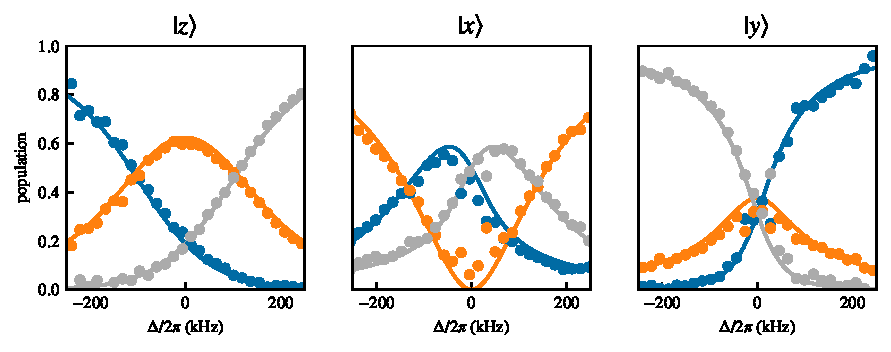
\includegraphics[]{Figures/Chapter6/figS11}
    \caption[State decomposition of the $\xyz$ states]{Decomposition of the $\xyz$ states on the $\ket{m_F}$ basis for $\Omega/2\pi=\SI{145(1)}{kHz}$
    The $\ket{m_F=-1,0,1}$ states correspond to blue, orange, gray respectively.}
    \label{fig:s1}
\end{figure*}

We labeled our dressed states $\xyz$ since for $\Omega\rightarrow 0^+$ and $\Delta=0$, they continuously approach the $\XYZ$ states familiar from quantum chemistry~\cite{cooper_reaching_2013}:
\begin{align}
    \ket X &= \frac{\ket{1} - \ket{-1}}{\sqrt{2}}, \nonumber \\
    \ket Y &= i\frac{\ket{1} + \ket{-1}}{\sqrt{2}}, \\
    \ket Z &= \ket{0}. \nonumber
\end{align}
which transform under the application of the spin-1 operators as $\epsilon_{jkl}\hat F_j \ket k= i\hbar \ket l$, so that a resonant probe field can induce transitions between at least one pair of states, irrespectively of its polarization.

Finally, when $\Omega\to\infty$ they are independent of the driving field amplitude and continuously approach the eigenstates of the $\hat F_x$ operator
\begin{align}
    \ket x &= \ket{1} - \ket{-1}, \nonumber \\
    \ket y &= \ket{1} + \sqrt 2 \ket 0 + \ket{-1}, \\
    \ket z &= \ket{1} - \sqrt 2 \ket 0 + \ket{-1}. \nonumber
\end{align}

\subsection{Energies}

The clock-like nature of these states is determined by their eigenvalues which are even functions with respect to $\Delta$ as can be seen by the leading order expansion of the eigenenergies $E_i=\hbar\omega_i$ for $\Delta\to 0$
\begin{align}
    \omega_x =& -\frac{\epsilon}{\Omega^2} \Delta^2 + \mathcal{O}(\Delta^4), \nonumber \\
    \omega_y =& \frac 12 (-\epsilon + \tilde\Omega) - \frac{(\epsilon + \tilde\Omega)}{-\epsilon^2-4\Omega^2+\epsilon\tilde\Omega} \Delta^2 + \mathcal{O}(\Delta^4), \label{eq:exp} \\
    \omega_z =& \frac 12 (-\epsilon - \tilde\Omega) + \frac{(\epsilon - \tilde\Omega)}{\epsilon^2+4\Omega^2+\epsilon\tilde\Omega} \Delta^2 \nonumber ,
\end{align}
where  we have defined $\tilde\Omega=\sqrt{4\Omega^2+\epsilon^2}$. The energy differences $\hbar\omega_{xy}$, $\hbar\omega_{zy}$ and $\hbar\omega_{zx}$ are only quadratically sensitive to $\Delta$ for $\Delta\ll\Omega$~\footnote{The energies are quadratic in $\Delta$ for $\Delta\ll\Omega$, and linear for $\Delta\gg\Omega$ with a slope of \SI{7}{MHz/mT}.} so that detuning fluctuations $\delta \Delta$ are suppressed to first order, making these a trio of synthetic clock states. The curvatures of $\omega_x$ and $\omega_z$ have the same sign and in principle there is a critical value of $\Omega$ where the quadratic term in transition energy can be made arbitrarily small, making it quartic in $\Delta$. However, this cancellation does not take place when we consider the dependence of $\epsilon$ on $\Delta$ from the Breit-Rabi expression. It is still possible to find an optimal $\Omega$ for which $\omega_{zx}$ depends quartically on $\Delta$, but it does not occur at $\Delta=0$ as is predicted by Equation~\ref{eq:exp} for constant $\epsilon$. 

\subsection{Transition matrix elements}
\label{sec:xyz_matrix_elements}

Unlike the $\ket{m_F}$ basis, an oscillatory magnetic field with the right polarization can drive transitions between all pairs of the $\xyz$ states with non-zero transition matrix elements. The transition matrix elements between the $\xyz$ have a dependence on both $\Omega$ and $\Delta$. For the $\Delta=0$ case they can be read from the representation of the spin-1 matrices in the $\xyz$ basis

\begin{align}
\fx &\rightarrow \begin{pmatrix}
 \frac{2 \Omega }{\tilde{\Omega}} & 0 & -\frac{\epsilon }{\tilde{\Omega}} \nonumber \\
 0 & 0 & 0 \nonumber\\
 -\frac{\epsilon }{\tilde{\Omega}} & 0 & -\frac{2 \Omega }{\tilde{\Omega}} \nonumber\\
\end{pmatrix} \nonumber \\ \nonumber\\
%
\fy &\rightarrow \begin{pmatrix}
 0 & -\frac{i (\tilde{\Omega} -\epsilon )}{\Omega  \sqrt{\frac{(\epsilon -\tilde{\Omega} )^2}{\Omega ^2}+4}} & 0 \nonumber\\
 \frac{i (\tilde{\Omega} -\epsilon )}{\Omega  \sqrt{\frac{(\epsilon -\tilde{\Omega} )^2}{\Omega ^2}+4}} & 0 & -\frac{i (\tilde{\Omega} +\epsilon )}{\Omega 
   \sqrt{\frac{(\tilde{\Omega} +\epsilon )^2}{\Omega ^2}+4}} \nonumber\\
 0 & \frac{i (\tilde{\Omega} +\epsilon )}{\Omega  \sqrt{\frac{(\tilde{\Omega} +\epsilon )^2}{\Omega ^2}+4}} & 0 \\
\end{pmatrix}  \nonumber\\ \nonumber\\
%
\fz &\rightarrow \begin{pmatrix}
 0 & -\frac{\sqrt{\frac{\epsilon }{\tilde{\Omega}}+1}}{\sqrt{2}} & 0 \\
 -\frac{\sqrt{\frac{\epsilon }{\tilde{\Omega}}+1}}{\sqrt{2}} & 0 & -\frac{2}{\sqrt{\frac{\left(\tilde{\Omega}+\epsilon
   \right)^2}{\Omega ^2}+4}} \\
 0 & -\frac{2}{\sqrt{\frac{\left(\tilde{\Omega}+\epsilon \right)^2}{\Omega ^2}+4}} & 0 \\
\end{pmatrix},
\label{eq:matrix_elements}
\end{align}
%
where the states have been ordered by decreasing energy ($\ket{y}$, $\ket{x}$, $\ket{z}$). We therefore see that a term in a Hamiltonian that is proportional to $\fx$ can only drive transitions between $\ket{z}$ and $\ket{y}$ and that a coupling term proportional to $\fy$ and $\fz$ can drive both drive transitions between $\ket{z}$ and $\ket{x}$ or $\ket{x}$ and $\ket{y}$ with different strengths. It can be seen from Equation~\ref{eq:matrix_elements} that when $\Omega$ and $\epsilon$ are comparable in magnitude there exists at least one non-zero transition matrix element for each pair of dressed states and they can all be coupled cyclically.

%  are nonzero and the states can be coupled cyclically.

% For $\Omega \ll \epsilon$ the matrix elements correspond to those of the $\ket{m_F}$ basis and $\langle x \vert \hat F_+ \vert y \rangle = 0$ as expected by angular momentum selection rules. When $\Omega$ and $\epsilon$ are comparable in magnitude al transition matrix elements are nonzero and the states can be coupled cyclically.

% \note{TODO: write matrix elements in dressed basis}
% As $\Omega \gg \epsilon$ the $\ket z$ and $\ket y$ states decouple and the system resembles an `undressed basis' following similar selection rules. \note{I'm not entirely sure how this were computed, I should redo this plots}

% \begin{figure*}[ht]
%     \centering
%     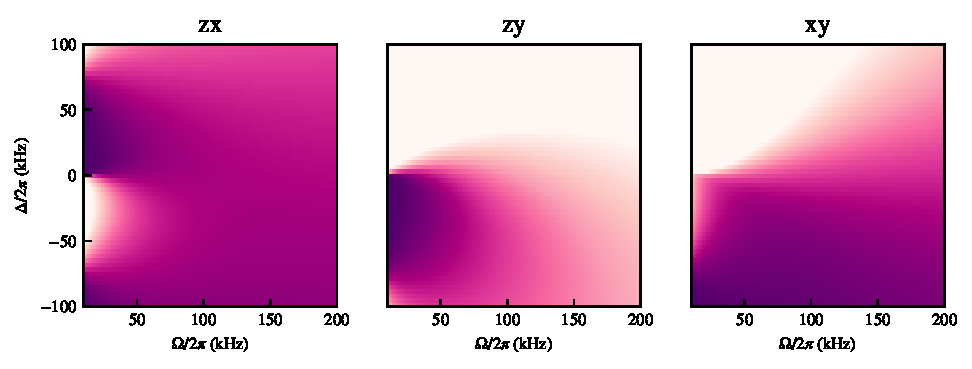
\includegraphics[]{Figures/Chapter6/figS12}
%     \caption[Transition matrix elements over $\Omega$ and $\Delta$.]{Transition matrix elements over $\Omega$ and $\Delta$.
%     There is an assymetry between coupling on the blue and red side of the resonance that corresponds to the counter- and co-rotating terms $\hat F_-$ and $\hat F_+$.}
%     \label{fig:s12}
% \end{figure*}

\section{$\xyz$ state preparation}
\label{sec:xyz_state_preparation}

We implemented CCD to BECs with $N\approx\num{5e4}$ atoms. For all of the experiments described in this Chapter the dipole trap had trapping frequencies of $(f_x,\, f_y,\, f_z) = (42(3),\, 34(2),\, 133(3))$\,Hz. We applied a $B_0 \approx \SI{3.27}{mT}$ bias field that lifted the ground state degeneracy, giving an $\omega_0/2\pi = \SI{22.9}{MHz}$ Larmor frequency, with a quadratic shift $\epsilon/2\pi=\SI{76.4}{kHz}$. We determined that the ambient magnetic field fluctuations were dominated  by contributions from line noise giving an RMS uncertainty $\delta\Delta/2\pi = g_F \mu_{\rm B}\delta B/h=\SI{0.67(3)}{kHz}$.

The state preparation consisted of two stages of ARP. On the first stage we followed the usual protocol described in Section~\ref{sec:arp} to prepare the BEC in any of the $\ket{m_F = 0,-1,1}$ states. On the second stage, we adiabatically transformed the $\ket{m_F}$ states into the $\xyz$ states. We started with the bias field far from resonance ($\Delta(t=0)/2\pi \approx -\SI{450}{kHz}$) and with all coupling fields off. Then we ramped on $\Omega$ in a two-step process. We first ramped from $\Omega=0$ to an intermediate value $\Omega_{\rm mid}$, approximately half its final value in \SI{1}{ms}. We then ramped $\Delta$ to zero in \SI{3}{ms} by increasing the magnetic field $B_0$. After allowing $B_0$ to stabilize for \SI{30}{ms}, we ramped the RF dressing field to its final value $\Omega$ in \SI{1}{ms}, yielding the dynamically decoupled $\xyz$ states. It was important that we waited for the field to stabilize at an intermediate $\Omega_{\rm mid}$ as we found several times that the capacitors on the impedance matching network of the antenna used to generate the RF field would burn if we kept the power on for too long.

After performing any experiment with the $\xyz$ states we measured their populations by adiabatically deloading them back into the $\ket{m_F}$ basis. We first ramped $B_0$ so that $\Delta$ approached its initial detuned value in \SI{2}{ms}, and then ramped off the dressing RF field in \SI{1}{ms}. A typical experimental sequence for $\Delta$ and $\Omega$ can be visualized in Figure~\ref{fig:ccd_protocol}. As usual, we obtained the spin-resolved momentum distribution using absorption imaging after TOF, with a  Stern-Gerlach field to spatially separate the spin components. The right panel of \reffig{fig:1}b shows a TOF image of the $\ket{m_F}$ state decomposition of the $\ket z$ state. For this image as well as for the measurement of the dressed state decomposition shown in Figure~\ref{fig:s1} we suddenly (not-adiabatically) turned the RF coupling off, thereby projecting the $\xyz$ states back into the $\ket{m_F}$ basis.
\begin{figure*}[ht]
    \centering
    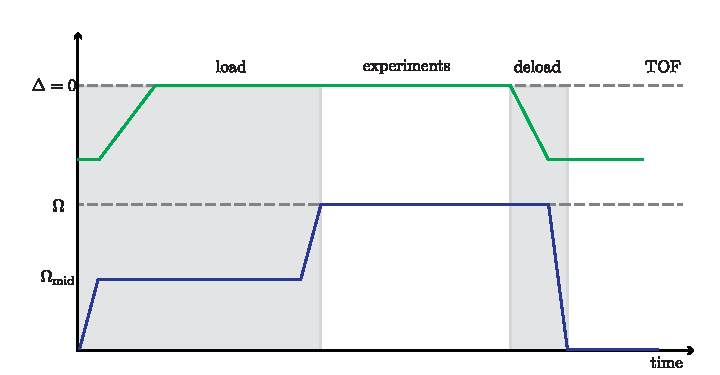
\includegraphics[]{Figures/Chapter6/loading_xyz_traces}
    \caption[Experimental CCD protocol]{Detuning and RF coupling strengths ramps (not to scale) performed to adiabatically prepare the $\xyz$ states starting in the $\ket{m_F}$ states and vice versa.}
    \label{fig:ccd_protocol}
\end{figure*}



\section{Initial characterization of $\Omega$}

Producing RF fields with large coupling strength was not a trivial task and when testing different antenna designs it was important to have an easy and quick way of characterizing them. We mostly relied on two different techniques to get an initial estimate of $\Omega$: first, we prepared atoms in $\ket{m_F=-1}$ and pulse on the RF to drive transitions between the three $\ket{m_F}$ states. We would then fit the populations in the three states as a function of pulsing time to the time evolution given the time dependent Sch\"odinger equation for the RF Hamiltonian (Equation~\ref{eq:h0}) with $\Omega$ and $\Delta$ as free parameters. 

\begin{figure*}[ht]
    \centering
    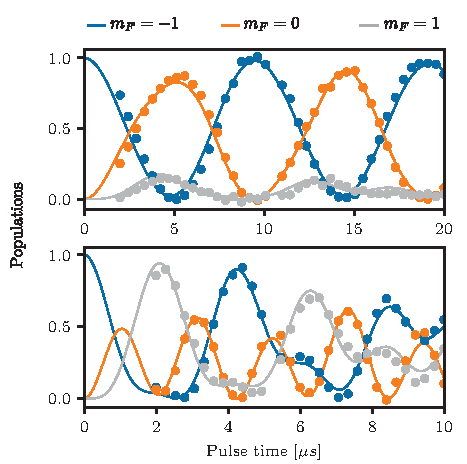
\includegraphics[]{Figures/Chapter6/Rabi_flop_calibrations.pdf}
    \caption[Calibration of $\Omega$]{We prepared the system in the $\ket{m_F=-1}$ state and pulsed $\Omega$ for variable times. We fit the populations in the $\ket{m_F}$ states as a function of pulsing time to get an initial estimate of $\Omega$. The top panel shows the time evolution of $\Omega/2\pi\approx\unit[76]{kHz}$ and the bottom panel shows the evolution for $\Omega/2\pi\approx\unit[238]{kHz}$}
    \label{fig:rabi_calibration}
\end{figure*}

Alternatively, we followed the loading procedure described in Section\ref{sec:xyz_state_preparation} but suddenly turned $\Omega$ off for different values of $\Delta$ to get the decomposition of the $\xyz$ states in terms of the $\ket{m_F}$ states. We then fit the populations to the eigenstates of the Equation~\ref{eq:h0} with $\Omega$ and $\Delta$ as free parameters. Figure~\ref{fig:s1} is an example of such type of calibration. 

For an antenna with a high quality factor such as ours ($q\sim20$) we could not `suddenly' turn $\Omega$ on or off as it takes some time for power to build up and to die out when the RF fields are turned on or off. If we did not include this into the model used to calibrate $\Omega$ we could get some results that were slightly off. We only used these measurements as initial estimates and once we found an antenna design that could produce a large enough $\Omega$ we used the spectroscopy techniques described in the next section to fully characterize the system. 

\section{Spectroscopy}
We confirmed our control and measurement techniques spectroscopically by measuring the energy differences between the $\xyz$ states with an additional probing field with angular frequency $\omega+\omega_p$, coupling strength $\Omega_p$ and polarized along $\ey$. In the frame rotating with angular frequency $\omega$ and after using a RWA the system was described by the Hamiltonian 
%
\begin{align}
    \hat H = \Delta\hat F_z &+ \hbar\epsilon(\hat F_z^2 / \hbar^2 - \hat{\mathbb I}) + \Omega \hat F_x \nonumber \\
    &+ \Omega_p \left(\sin(\omega_p t) \hat F_x + \cos(\omega_p t) \hat F_y\right).
    \label{eq:h}
\end{align}
%
In this rotating frame the probe field initially polarized along $\ey$ has components along $\ex$ and $\ey$, resulting in at least one non-zero transition matrix element for all transitions between pairs of dressed states. If the probing field was polarized along $\ez$ we would not be able to drive the $zy$ transition as can be seen from the matrix elements in Equation~\ref{eq:matrix_elements}.

To probe the dependence of the $\xyz$ state energies on detuning, we performed Rabi spectroscopy (Section~\ref{sec:Rabi_oscillations}) by pulsing $\Omega_p$ on for a constant time and scanned $\omega_p$ for different values of $\Delta$. Figure~\ref{fig:1}b shows the spectroscopically resolved values of $\omega_{xy}/2\pi$, $\omega_{yz}/2\pi$, and $\omega_{zx}/2\pi$ for $\Omega/2\pi=\SI{194.5(1)}{kHz}$ and the side panel shows a sample spectra measured with coupling strength $\Omega_p/2\pi \approx \SI{1}{kHz}$ and $\Delta/2\pi \approx \SI{9}{kHz}$. The dashed curves were computed by diagonalizing \refeq{eq:h0}, and they clearly depart from our measurements for the $zx$ transition.
This departure results from neglecting the weak dependence of the quadratic shift $\epsilon$ on bias field $B_0$. In near-perfect agreement with experiment, the solid curves from the full Breit-Rabi expression account for this dependency.
%
\begin{figure*}[ht]
    \centering
    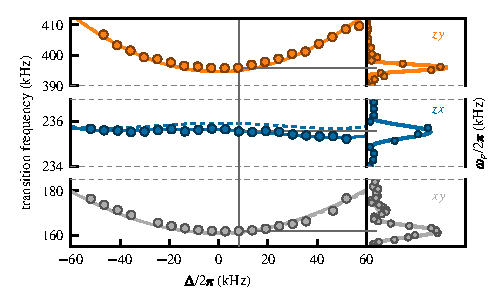
\includegraphics[]{Figures/Chapter6/fig1b}
    \caption[Spectroscopy of the $\xyz$ states]{Left: spectroscopic data showing transitions between the $\xyz$ states for $\Omega/2\pi = \SI{194.5(1)}{kHz}$.
    The vertical scale of the center panel ($zx$ transition) has only $10\%$ the range of the other panels. The dashed lines correspond to the Hamiltonian of \refeq{eq:h0} while the solid lines include the dependence of the quadratic shift on $\Delta$.Right: representative spectra.}
    \label{fig:xyz_spextroscopy}
\end{figure*}
%
\begin{figure}[!!h]
    \centering
    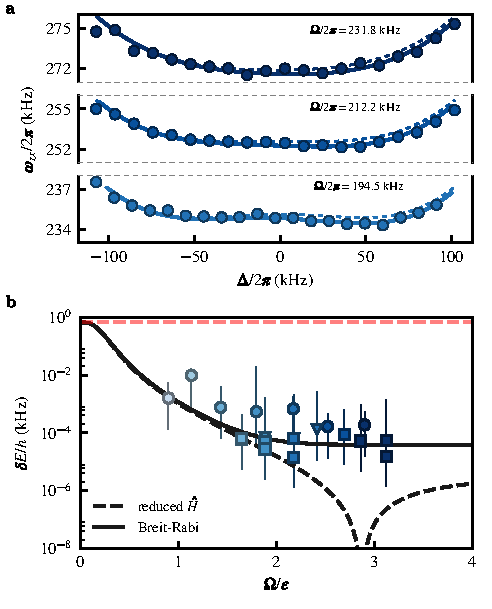
\includegraphics[]{Figures/Chapter6/fig2.pdf}
    \caption[The $\ket{z}\rightarrow\ket{x}$ transition as a function of $\Omega_{\rm RF}$]{{\bf a.} Transition frequency $\omega_{zx}/2\pi$ for three values of $\Omega/2\pi$.
    The dashed curves correspond to \refeq{eq:h}, while the solid curves use the Breit-Rabi expression.
    {\bf b.} The change in energy from our experimental detuning fluctuations as measured in the $\ket{m_F}$ basis is $\delta \Delta/2\pi = \SI{0.67}{kHz}$ (red dashed line).
    Triangles correspond to $\xyz$ spectroscopy data, squares to side-of-peak $\pi$-pulse data, and circles to double-dressed data.
    The black dashed (solid) curve was calculated using \refeq{eq:h} (the Breit-Rabi expression).
    The shading of the data points corresponds to the Rabi frequencies in \reffig{fig:3}.}
    \label{fig:2}
\end{figure}

\section{Robustness}
We focus on the robustness of the $zx$ transition which can be made virtually independent of magnetic field variations due to the similar curvature of $\omega_z(\Delta)$ and $\omega_x(\Delta)$ (see the middle panel of \reffig{fig:1}b). We quantified the sensitivity of this transition to field variations with three methods corresponding to the different markers in \reffig{fig:2}b:
(1) Triangles denote data using Rabi spectroscopy as in \reffig{fig:2}a.
(2) Squares denote data in which a detuned $\pi$-pulse of the probe field transferred approximately half of the atoms from $\ket z$ to $\ket x$. This `side-of-peak' technique overcomes the limitation of Rabi spectroscopy being first-order insensitive to changes in $\omega_{zx}$.
(3) Circles describe data using a double dressing technique that will be described in Section~\ref{sec:concatenated_cdd}.
In each case we measured the energy shift from resonance as a function of detuning (magnetic field) and then used a fourth-order polynomial fit to extract the RMS residuals $\delta \omega_{zx}$ due to the known detuning noise~\footnote{Our procedure also quantifies the small fluctuations that survive for spectra that are flat beyond second order, as in \refeq{eq:h0}.}. The results are not consistent with the theory simple from \refeq{eq:h} (dashed) and instead require the Breit-Rabi expression (solid) to obtain full agreement~\footnote{The fluctuations can be even smaller for a given $\Omega$ if we allow for $\Delta \neq 0$.}.

Even at our smallest coupling $\Omega/2\pi=\SI{69(1)}{kHz}$ the typical magnetic field noise was attenuated by two orders of magnitude, rendering it essentially undetectable. Ideally, the radius of curvature of $\omega_{zx}(\Delta)$ changes sign at about $\Omega/2\pi = \SI{220}{kHz}$, leaving only a $\Delta^4$ contribution, however, in practice the small dependence of $\epsilon$ on $B$ prevents this perfect cancellation. Still it is possible to see the changing curvature of $\omega_{zx}(\Delta)$ near $\Delta=0$ for different values of $\Omega$ in Figure~\ref{fig:2}a.

\subsection{Optimal response to noise}

The sensitivity of the $zx$ transition to detuning fluctuations can be optimized further by working at $\Delta \neq 0$ as shown in \reffig{fig:sopt}.
%This behavior can only be captured by including the dependence of the quadratic shift on $\Delta$ as given by the Breit-Rabi expression.

For small values of $\Omega$, the optimum value of $\Delta$ corresponds to one of the concave features of the $zx$ transition energy that arises due to the asymmetry introduced by the quadratic shift.
As $\Omega$ gets larger, these features merge into a single one and the optimum value is $\Delta \approx 0$.
The deviation from $\Delta=0$ is due to an overall tilt of the transition energy coming from the dependence of the quadratic shift on $\Delta$.
At the optimum point $\Omega/\epsilon \approx 3$ the sensitivity of the synthetic clock transition is \SI{1.9e-07}{kHz}, c.f, the $\Rb87$ clock transition which scales as \SI{57.5}{kHz/mT^2} and gives \SI{5.8e-07}{kHz}.
\begin{figure*}[ht]
    \centering
    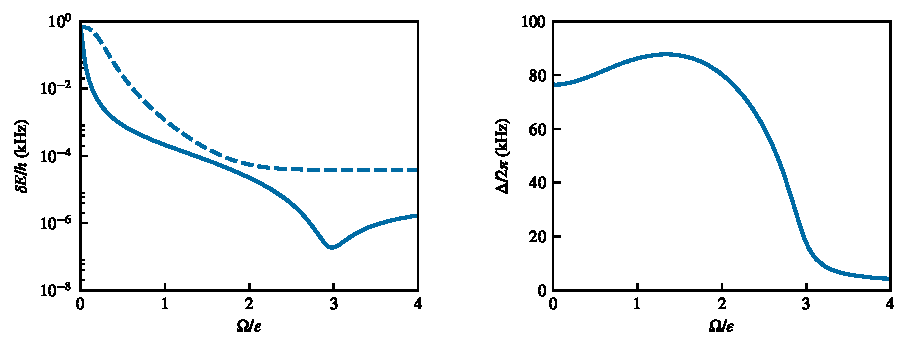
\includegraphics[]{Figures/Chapter6/figS13}
    \caption[Optimal response of the $zx$ transition]{Left: Optimum response (solid) of the $zx$ transition to detuning fluctuations allowing for finite $\Delta$ compared to $\Delta=0$ (dashed) for the full Breit-Rabi model.
    Right: The values of $\Delta$ that correspond to the minimum derivative of $\omega_{zx}$.}
    \label{fig:sopt}
\end{figure*}

\section{Driving dressed state transitions}
\begin{figure}[ht]
    \centering
    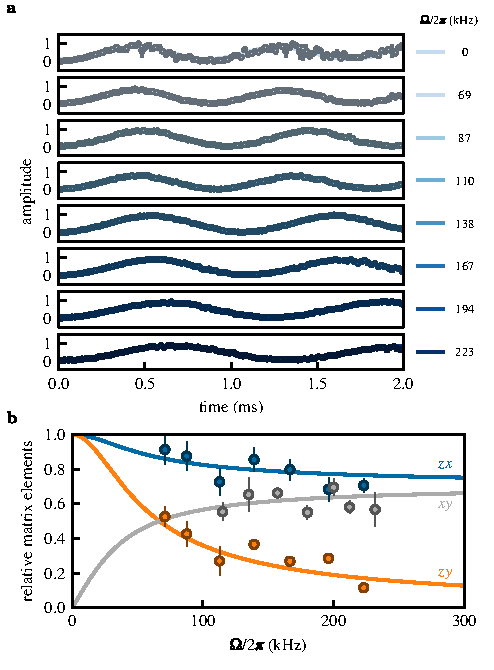
\includegraphics[]{Figures/Chapter6/fig3.pdf}
    \caption[Coherent driving of dressed state transitions]{{\bf a.} Rabi oscillations.
    Phase coherence is maintained throughout the oscillations in the dressed basis, while it is quickly lost in the $\ket{m_F}$ basis.
    The marker size reflects the typical uncertainties on the dressed basis oscillations.
    {\bf b.} Transition matrix elements for $zx$ (blue) and $zy$ (orange) transitions decrease monotonically with increasing $\Omega$ for $\Delta=0$, while they increase for $xy$.
    }
    \label{fig:3}
\end{figure}
We explored the strength of the probe-driven transitions between these states by observing coherent Rabi oscillations (\reffig{fig:3}a) where our BEC was prepared in $\ket z$ and the probe field had strength $\Omega_p/2\pi\approx\SI{1}{kHz}$.
The top panel shows Rabi oscillations between $\ket{m_F=0}$ and $\ket{m_F=-1}$ states for reference, and the remaining panels show oscillations between $\ket{z}$ and $\ket{x}$.
The observed Rabi frequency between dressed states decreased with increasing $\Omega$ indicating a dependence of the $zx$ transition matrix elements on $\Omega$. We repeated this experiment driving all possible pairs of dressed state transitions at fixed $\Omega_p$ for,  and \reffig{fig:3}b shows the dependence of these matrix elements on $\Omega$ for $\Delta=0$.

The coherence of the Rabi oscillations for longer times was limited by gradients in $\Omega$ that lead to phase separation of the dressed states, and therefore loss of contrast in the oscillations. This effect was faster for smaller frequency Rabi oscillations. For example for $\Omega_p/2\pi=\unit[5]{kHz}$ we observed coherent Rabi oscillations with almost full contrast for more than $\unit[10]{ms}$ while for the $\Omega_p/2\pi=\unit[870]{Hz}$ oscillation shown in Figure~\ref{fig:decaying_rabi} the contrast was significantly reduced after $\unit[5]{ms}$. The loss of contrast was even worse when we tried performing a Ramsey sequence where the time evolution is most sensitive to the environment. One solution to this problem would be to change the experimental setup to a double loop antenna to generate a more spatially uniform magnetic field. 
%
\begin{figure}[ht]
    \centering
    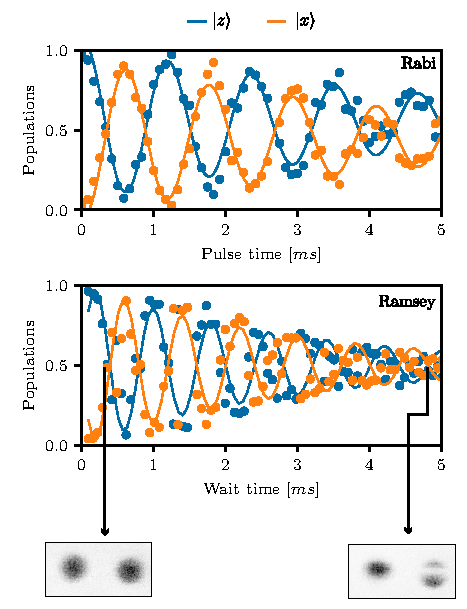
\includegraphics[]{Figures/Chapter6/RF_Ramsey.pdf}
    \caption[Loss of contrast of coherent oscillations]{Loss of contrast in coherent oscillations. A Rabi oscillation (top) between the $\ket{z}$ and $\ket{x}$ states with $\Omega_p/2\pi=\unit[870]{Hz}$ decays by $1/e$ in $\unit[4.6]{ms}$ and a Ramsey oscillation (middle) with about $\unit[1]{kHz}$ frequency decays in about $\unit[3]{ms}$. The gradients in $\Omega$ lead to phase separation of dressed states and loss of contrast for longer pulse/wait times.  
    }
    \label{fig:decaying_rabi}
\end{figure}

In comparison, we found that for both Rabi and Ramsey oscillations between the $\ket{m_F}$ states the phase started deteriorating after a few hundreds of $\us$, this is not surprising due to bias magnetic field temporal noise. We canceled gradient magnetic fields so that no phase separation of the bare states was observed for $>\SI{10}{sec}$. As a result, the system can in principle undergo coherent evolution without loss of contrast for a long time but because of field fluctuations between shots what we observed instead was full contrast noise. 

\section{Concatenated CDD }
\label{sec:concatenated_cdd}
The driving field $\Omega$ coupled together the $\ket{m_F}$ states, giving us the $\xyz$ synthetic clock states that were first-order insensitive to magnetic field fluctuations. However, the spectrum of these states is still first-order sensitive to fluctuations of the driving field $\delta \Omega$. Reference~\cite{cai_robust_2012} showed that an additional field coupling together with these $\xyz$ states can produce doubly-dressed states that are insensitive to both $\delta \Omega$ and $\delta \Delta$: a process called concatenated CDD.
In our experiment, the probe field provided the concatenating coupling field. 
Because $\Omega_p\ll\Omega$, we focus on a near-resonant two-level system formed by a single pair of dressed states, here $\ket{z}$ and $\ket{x}$, which we consider as pseudospins $\ket{\!\uparrow}$ and $\ket{\!\downarrow}$.
These states are described by the effective two-level Hamiltonian
\begin{equation}
    \hat H_p = \frac{\hbar\Delta'}{2} \hat \sigma_3 + \hbar\Omega' \cos(\omega_p t) \hat \sigma_1,
    \label{eq:h2}
\end{equation}
with energy gap $\Delta' \approx \omega_{z,x}$ (shifted by off-resonant coupling to the $zy$ and $xy$ transitions) and coupling strength $\Omega' \propto \Omega_p$, as set by the matrix elements displayed in~\reffig{fig:3}b.
Here $\hat \sigma_{1,2,3}$ are the three Pauli operators.

We perform a second transformation into a frame rotating with angular frequency $\omega_p$ and use a RWA to compute the eigenenergies of Equation~\ref{eq:h2}. For large values of $\Omega'$ the energies take the values $E_{\uparrow,\downarrow} \approx \pm\Omega^\prime/2 + (\Delta^\prime)^2/2\Omega^\prime$. Even though $E_{\uparrow,\downarrow}$ are still first order sensitive to $\Omega$ because $\Delta'\approx\omega_{z,x}\propto\Omega$, its effect is suppressed by a factor of $1/\Omega'$. Thus, the concatenated CDD field protects from the fluctuations $\delta\Delta^{\prime}$ of the first dressing field in a similar way that CDD provided protection from detuning noise $\delta \Delta$. Table~\ref{table:CDD} summarizes the dependence of the $\xyz$ and $\ket{\uparrow\downarrow}$ energies on $\Delta$, $\Omega$ and $\Omega'$. 
%
\begin{table}[h]
\caption[Summary of CDD energies]{Energies of the CDD and CCDD states as a function of $\Delta$, $\Omega$ and $\Omega'$. The dependence on parameters not relevant to the expansion is given by the functions $f_1$, $f_2$, $g_1$ and $g_2$.}
\begin{center}
\begin{tabular}{c|c|c}
\hline
 % & & \\
 & CDD & concatenated CDD \\
 % & & \\
\hline \hline
 % & & \\
$\Delta$ dependence  & $f_1(\epsilon,\Omega)\Delta^2$ & $f_2(\Omega,\epsilon)\frac{\Delta^2}{\Omega'}$ \\
 & & \\
\hline
 % & & \\
$\Omega$, $\Omega'$ dependence & $\Omega+g_1(\Delta, \epsilon)\frac{1}{\Omega}$ &  $\left[\Omega^2 + \epsilon\Omega + g_2(\Delta, \epsilon)\frac{1}{\Omega}\right]\frac{1}{\Omega'}$ \\
 & & \\  
% \hline
\end{tabular}
\end{center}
\label{table:CDD}
\end{table}

We produced doubly-dressed states by doing (one more!) ARP sequence. We initialized the system in the $\ket{\!\downarrow}$ state with RF coupling strength $\Omega_i$. We set the probe frequency to be $\sim\unit[20]{kHz}$ off resonant with respect to the $\ket{\, \downarrow}\rightarrow \ket{\, \uparrow}$ transition and ramped it on in $\unit[10]{ms}$. We then ramped $\Omega_i\rightarrow\Omega_f$ in $\unit[30]{ms}$. The experimental sequence can be visualized in Figure~\ref{fig:concatenated_cdd}. We chose the value of $\Omega_f$ such that it would bring $\omega_p$ to resonance at $\Delta=0$, creating double dressed states that were equal superposition of $\ket{\,\downarrow}$ and $\ket{\,\uparrow}$. We quantified the sensitivity of this transition to large changes in the detuning $\Delta$ in terms of the fractional population imbalance $\langle\hat\sigma_3\rangle = P_\downarrow(\Delta)-P_\uparrow(\Delta)$, shown in \reffig{fig:4}a for $\Omega_f/2\pi=\SI{138.2(1)}{kHz}$~\footnote{We chose the maximum value of $\Delta$ such that the population of \unexpanded{$\ket y$}, was negligible after deloading.}.
This signal is first-order sensitive to $\omega_{\downarrow, \uparrow}$, and provided our third measurement of sensitivity to detuning in \reffig{fig:2}b denoted by circles.
\begin{figure}[!ht]
    \centering
    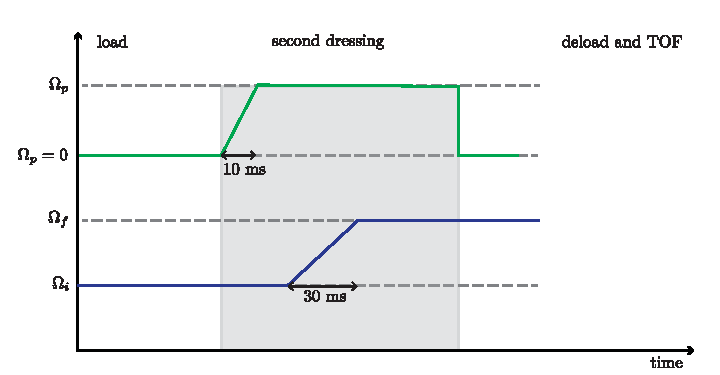
\includegraphics[]{Figures/Chapter6/concatenated_cdd.pdf}
    \caption[Concatenated CDD protocol]{Experimental protocol for implementing concatenated CDD. We started an initial RF coupling strength $\Omega_i$ and ramped on the probe field $\Omega_p$ in a few ms with $\omega_p=\omega_{z,x}(\Omega_f)$ so that it was initially slightly off resonant with the $zx$ transition. We then ramped the RF field to $\Omega_f$, brining $\omega_p$ to resonance. 
    }
    \label{fig:concatenated_cdd}
\end{figure}
\begin{figure}[h]
    \centering
    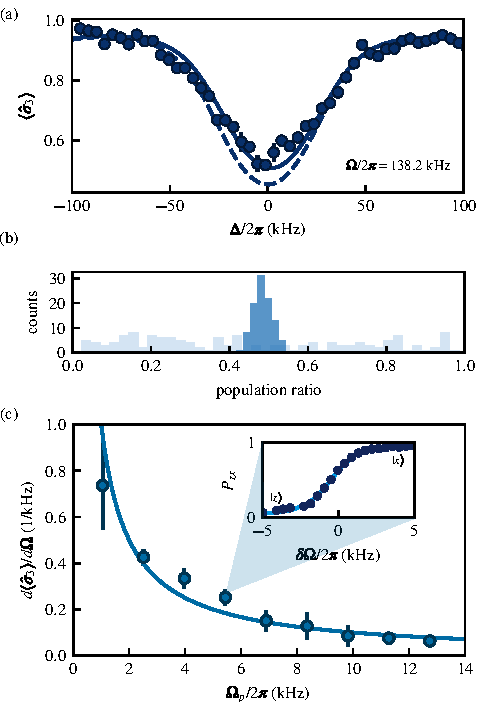
\includegraphics[]{Figures/Chapter6/fig4.pdf}
    \caption[Concatenated CCD]{(a) The fractional population imbalance of the $\downarrow\uparrow$ transition for $\Omega/2\pi=\SI{138.2(1)}{kHz}$ over detuning $\Delta$.
    The dashed curve is calculated using \refeq{eq:h} and the solid one using the full Breit-Rabi expression.
    (b) The fidelity of preparing a balanced superposition of $\ket{\!\downarrow}$ and $\ket{\!\uparrow}$ (dark blue) states compared to $\ket{m_F=0}$ and $\ket{m_F=-1}$ states (light blue).
    (c) The robustness of $\downarrow, \uparrow$ transition against fluctuations $\delta \Omega$ for different probe field coupling strengths.
    The points represent the slope of the fitted curves to the fractional population imbalance (inset).}
    \label{fig:4}
\end{figure}

We compared the fidelity of preparing a superposition of the $\ket{\,\downarrow}$ and $\ket{\,\uparrow}$ states to adiabatically preparing a similar superposition of the the $\ket{m_F=0}$ and $\ket{m_F=-1}$ states using a single ARP (no dressed states involved), both with a probe field strength of  $\approx\SI{1}{kHz}$.
Figure~\ref{fig:4}b shows the RMS deviation of the population imbalance measured over a few hundred repetitions of the experiment.
The RMS deviation for the dressed basis is $0.024(1)$ and is an order of magnitude smaller than for the $\ket{m_F}$ basis $0.29(1)$, where it practically impossible to prepare a balanced superposition for the parameters used here~\footnote{In \reffig{fig:4}b, the noise in the $\ket{m_F}$ basis is not Gaussian distributed as is typical of line noise in these experiments.}.

Figure~\ref{fig:4}c shows the response of the $\ket{\, \downarrow}\rightarrow \ket{\, \uparrow}$ transition to small changes $\delta\Omega$ for different values of $\Omega_p$.
We prepared an equal superposition of $\ket{\,\downarrow}$ and $\ket{\,\uparrow}$ following the same procedure as before for $\Omega_f/2\pi = \SI{138.2(1)}{kHz}$.
We then measured how the population imbalance changes for small variations of $\Omega$ --- the effective detuning in the `twice-rotated frame' --- for different probe amplitudes $\Omega_p$.
We defined a sensitivity parameter $d\langle\hat\sigma_3\rangle / d\Omega$, obtained from the linear regime of the population imbalance measurements (see inset in \reffig{fig:4}c).
The robustness of the doubly-dressed states against $\delta \Omega$ fluctuations increased with $\Omega_p$, thus verifying the concatenating effect of CDD in the $\xyz$ basis.

However promising the application of multiple concatenating fields might seem, this procedure has a fundamental limitation. Each time a new coupling field is applied the energies of the dressed states are reduced to something on the order of magnitude of the coupling strength from the applied concatenating field. For example, in the experiments we described here we started with $\ket{m_F}$ states with transition frequencies on the order of MHz. The transition frequencies of the $\ket{xyz}$ states were reduced to hundreds of kHz (or in general the magnitude of $\Omega$). After applying the second concatenating RF field the transition frequencies of the $\ket{\!\downarrow\uparrow}$ are of the order of $\Omega_p\sim\unit[10]{kHz}$ which needs to be smaller than $\Omega$ for the second RWA to be valid. Therefore we see that after applying multiple concatenating fields we are at the risk of having some very robust states that are also very closely spaced in energy which might not be desirable for some applications. 

\section{Conclusions}
We realized a three-level system that is dynamically decoupled from low-frequency noise in magnetic fields, measured now-allowed transitions between all three states, and demonstrated control techniques for creating arbitrary Hamiltonians.  These techniques add no heating or loss mechanisms, yet within the protected subspace retain the full complement of cold-atom coherent control tools such as optical lattices and Raman laser coupling, and permit new first-order transitions that are absent in the unprotected subspace.
These transitions enable experiments requiring a fully connected geometry as for engineering exotic states, e.g., in cold-atom topological insulators, and two-dimensional Rashba spin-orbit coupling in ultracold atomic systems~\cite{campbell_rashba_2016, juzeliunas_generalized_2010}.

The synthetic clock states form a decoherence-free subspace that can be used in quantum information tasks where conventional clock states might be absent, or incompatible with other technical requirements~\cite{bacon_universal_2000}.
Moreover, their energy differences are proportional to the amplitude of the dressing field, and hence tunable, so they can be brought to resonance with a separate quantum system.
The effective quantization axis can be arbitrarily rotated so that the two systems can be strongly coupled, pointing to applications in hybrid quantum systems~\cite{solano_chapter_2017,xiang_hybrid_2013}.
Introducing a second coupling field shields the system from fluctuations of the first, a process that can be concatenated as needed.
More broadly, synthetic clock states should prove generally useful in any situation where fluctuations of the coupling field can be made smaller than those of the environment.

% \section{Locating field resonance}

% We used an iterative procedure to measure and adjust the value of the detuning $\Delta$ to account for the weak response of the $\xyz$ states to detuning variations.
% As most of our experiments were done at $\Delta=0$, we first obtained an estimate of $\Delta$ from the imbalance of $\ket 1$ and $\ket{-1}$ populations from the decomposition of $\ket z$ which should be zero for $\Delta=0$ (see \reffig{fig:s1}).
% We then located the transition frequencies for at least two transitions (usually $zx$ and $zy$ as shown in \reffig{fig:s2}) using an ARP protocol as described in the main text and varying the frequency of the probe field.
% These frequencies correspond to a unique pair of $\Omega$ and $\vert\Delta\vert$ values which can then be used to adjust the bias magnetic field $B_0$ so that $\Delta=0$.
% However, there is an ambiguity as to the sign of $\Delta$ since the eigenstates are even functions of $\Delta$.

% We selected a direction randomly and subsequently verified if $\Delta=0$ using another set of spectroscopic measurement.
% We fixed the value of the probe field to be a few kHz above the transition frequency corresponding to $\Delta=0$ and used the same ARP sequence to transfer atoms from $\ket z$ to $\ket x$.
% This procedure gave two resonant values for $\Delta$ were atom transfer takes place, and the value where $\Delta=0$ corresponded to their mean (see \reffig{fig:s2}).
% Finally, we remeasured the $zx$ and $zy$ transition frequencies to validate that $\Delta=0$.
% For higher values of $\Omega_R$, using the $zx$ transition becomes impractical
% due to its insensitivity to detuning, and we followed the same procedure but using the $xy$ transition instead.










			% !TEX root = mainthesis.tex
%Chapter 7

\renewcommand{\thechapter}{7}

\chapter{Topological order in quantum systems}
\label{ch:Topology}

Topological order can be found in a wide range of physical systems, from crystalline solids\cite{hasan_colloquium:_2010}, photonic meta-materials\cite{ozawa_topological_2019} and even atmospheric waves\cite{delplace_topological_2017} to optomechanic\cite{peano_topological_2015}, acoustic\cite{yang_topological_2015} and atomic systems\cite{cooper_topological_2019}. Topological systems are a robust foundation for creating quantized channels for transporting electrical current, light, and atmospheric disturbances. These topological effects can be quantified in terms of integer-valued invariants such as the Chern number, applicable to the quantum Hall effect\cite{thouless_quantized_1982,haldane_model_1988}, or the $\mathbb{Z}_2$ invariant suitable for topological insulators\cite{kane_$z_2$_2005}. 

The topology of Bloch bands defines integers that serve to both classify crystalline materials and precisely specify properties, such as conductivity, that are independent of small changes to lattice parameters\cite{hasan_colloquium:_2010}. Topologically non-trivial materials first found application in metrology with the definition of the von Klitzing constant as a standard of resistance, which is now applied in the realization of the kilogram\cite{newell_codata_2018}. Today, topological systems have found applications in the engineering of low loss optical waveguides\cite{ozawa_topological_2019} and present a promising path to quantum computation\cite{nayak_non-abelian_2008}.

We got interested in topology when working on engineering Rashba~\cite{bychkov_oscillatory_1984} type spin-orbit coupling in the lab. Our system had non-trivial topology but it broke from the usual mold of topological materials as it didn't have an underlying crystalline structure that conventionally yields to integer Chern numbers. 

Before describing our experiments that characterize the unconventional topology of a Rashba spin-orbit coupled gas, in this Chapter I take a step back to describe the basic concepts of topology and its applications to the band theory of solids. The ideas of topology and how exactly one can connect donuts with band structures might feel a bit obscure and complicated for non-experts in the field. I wrote this Chapter with that in mind, with the hope that it can be followed by non-experts and provide some insight and intuition about this field. The concepts introduced in this Chapter will be necessary for understanding the results presented in Chapter~\ref{ch:Rashba}.
 
\section{Topology in mathematics} 

Topology is a branch of mathematics that studies continuity~\cite{differential_topology_and_geometry}. The most familiar example might be that of objects being continuously deformed into one another. For example, a donut can be continuously deformed into a coffee mug but if we want to deform it into a pretzel we need to poke more holes in it. This gives us some intuition that the donut and the mug must share the same topology, which is different from that of the pretzel. Topology also studies more abstract objects but I will limit the discussion to closed two-dimensional surfaces in three dimensions, which will be enough to provide some intuition when we define topological invariants for band structures in the following sections.  

The topology of 2D surfaces can be classified by the Euler characteristic, and it is related to the local Gaussian curvature of a surface by the Gauss-Bonet theorem. The Gaussian curvature can be interpreted in the following way: at any point in a surface we can find a normal vector which is orthogonal to the tangent plane of the surface. We can then define a family of planes containing the normal vector and their intersection with the surface defines a family of curves. The curvature of a any of these curves at the point where the planes intersect, which is equal to the quadratic coefficient in a Taylor expansion around that point, is called the normal curvature $\kappa$. When we consider all the normal curvatures, the minimum and maximum of these are called the principal curvatures and are used to define the Gaussian curvature at any point of a surface $K=\kappa_{min}\kappa_{max}$~\cite{differential_topology_and_geometry} 

The Gauss-Bonnet theorem states that the integral of the local Gaussian curvature over the whole surface is equal to the integer valued Euler characteristic
%
\begin{equation}
	\chi = \frac{1}{2\pi}\int_S K dA,
	\label{eq:euler_characteristic}
\end{equation}
%
which is related to the genus $g$ (number of holes or handles in the surface) by $\chi=2(1-g)$. The Gauss-Bonnet theorem is a very powerful result as it relates the local properties of a surface,the Gaussian curvature, with a global topological invariant, the Euler characteristic. \note{Add picture to describe principal curvatures?}

In the following sections I will introduce topological invariants in the context of condensed matter physics, which even though might seem a bit more abstract, their interpretation can be closely related to the concepts just defined in this section. 
\section{Topological order in condensed matter}

Just like topology classifies properties of geometric objects, one important task of condensed matter physics has been to classify phases of matter. Many of these phases, for example magnetic or conducting phases, can be described in terms of order parameters related to spontaneously broken symmetries~\cite{landau_theory_1936}. However, in the past few decades and increasing number of systems have been found where it is only possible to understand their phases and properties in terms of the underlying topology of their quantum states. This new paradigm of physics has been so important that in 2016 the Nobel prize in physics was awarded to David J. Thoules, F. Duncan M. Haldane and J. Michael Kosterlitz for the theoretical discoveries of topological phase transitions and topological phases of matter 

The effects of topology in condensed matter systems were first observed when von Klitzing and colleagues~\cite{klitzing_new_1980} measured the quantized Hall resistance in two-dimensional electron gases subjected to a strong perpendicular magnetic field. The effect can be understood semi-classically by thinking of the electrons' quantized cyclotron orbits\footnote{This is an intuitive but not very complete explanation of the quantum Hall effect, see \cite{tong_lectures_2016} if you want to learn more about this subject.} that give rise to Landau levels. If the Landau levels are filled then there is an energy gap separating two consecutive levels and the material acts as an insulator but if an electric field is applied the orbits drift and the electrons will be `skipping orbits' in the edge as can be seen in Figure~\ref{fig:quantum_hall}, giving rise to what is known as edge states.
% 
\begin{figure*}[htb]
\begin{center}
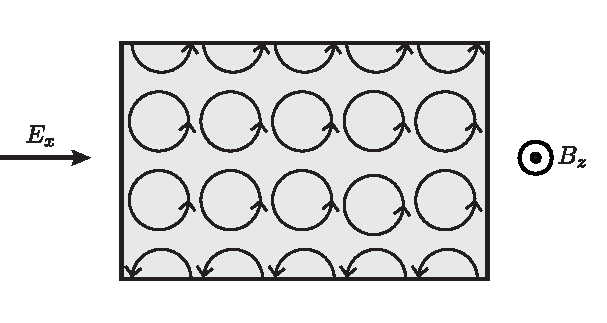
\includegraphics[]{Figures/Chapter7/quantum_hall.pdf}
\caption[The quantum Hall effect]{The quantum Hall effect. An electron gas is confined in a two-dimensional material and a strong magnetic field is applied perpendicular to the plane. The electrons on the bulk travel in cyclotron orbits while the electrons on the edge travel `skipping orbits'.}
\label{fig:quantum_hall}
\end{center}
\end{figure*}

In a seminal paper Thoules, Kohomoto, Nightingale, and den Nijs~\cite{thouless_quantized_1982} explained that the quantization of the Hall conductivity is determined by the underlying topology of the band structure. Just like the Euler characteristic defined in Equation~\ref{eq:euler_characteristic} classifies 2D solids that can be continuously deformed without opening or closing holes, there is a topological invariant that classifies band structures that can be deformed into one another without opening or closing an energy gap. This invariant, initially known as the `TKNN invariant', was later recognized by the mathematical physicist Bary Simon as the `first Chern class invariant from $U(1)$ fiber bundles'~\cite{simon_holonomy_1983}\footnote{See~\cite{geometry_topology_physics} if you want to dive into hardcore topology.} and the TKNN invariant became what is known today as the Chern number or Chern invariant. Another very valuable contribution from Simon's work was that he made the connection between the Chern number and the the Berry's geometrical phase~\cite{berry_michael_victor_quantal_1984} which will be defined in the following sections and will allow us to make a physical interpretation of this otherwise abstract seeming topological invariant. 

\section{Berry phase and Berry curvature}
\label{sec:Berry phase and curvature}

A Berry or geometric phase is used to describe the phase acquired by a quantum state as it moves through a closed trajectory in parameter space. It plays a key role in topological band theory and can help provide a physical interpretation of the Chern number. 

Consider a Hamiltonian $\hat H$ that depends on a set of parameters $\r=(r_1, r_2, ...)$. If the parameters are slowly changed in time, the corresponding change in the system can be described by a path in parameter space $\r(t)$. The state $\ket{\psi(t)}$ evolves according to the time dependent Sch\"odinger equation and at any given time $t$ there is a basis that satisfies
%
\begin{equation}
	\hat H(\r)\ket{n(\r)}=E_n(\r)\ket{n(\r)}
	\label{eq:hamiltonian_eigenvectors}
\end{equation}
%
for $\r=\r(t)$. Suppose the system is initially in state $\ket{n(\r(t=0))}$, if the parameters are changed slowly such that the adiabatic theorem is valid, then at time $t$ the state of the system can be written as
%
\begin{equation}
	\ket{\psi(t)}=\exp\Big\{-\frac{i}{\hbar}\int_0^tdt'E_n(\r(t'))\Big\}\exp(i\gamma_n(t))\ket{n(\r(t))},
	\label{eq:berry_wf}
\end{equation}
%
where the first exponential term corresponds to a dynamical phase factor, and the second term is a geometric phase. By imposing that $\ket{\psi(t)}$ satisfies the time-dependent Schr\"odinger equation one finds that 
%
\begin{equation}
	\gamma_n(t)=i\braket{n(\r)}{\nabla_{\r}n(\r)}\cdot\dot{\r}(t),
\end{equation}
%
where the term
%
\begin{equation}
	\mathbf{A}_n(\r)=i\braket{n(\r)}{\nabla_{\r}n(\r)}
	\label{eq:berry_connection}
\end{equation}
%
 is usually referred to as the Berry connection\footnote{This is related to the connection defined in differential geometry that is used to describe things like parallel transport.} or the Berry vector potential for reasons that will become apparent. Because eigenvectors can only be defined up to a global phase, $\mathbf{A}$ is a gauge dependent quantity. If we make a gauge transformation such that $\ket{n(\k)}\rightarrow\e^{i\xi(\k)}\ket{n(\k)}$ then the Berry connection is also transformed as $\mathbf{A}_n(\k)\rightarrow\mathbf{A}_n(\k)-\nabla_{\k}\xi(\k)$. However if we integrate the Berry connection on a closed loop
%
\begin{equation}
	\gamma_n(\mathcal{C})=\oint_{\mathcal{C}} \mathbf{A}_n(\r)\cdot d\mathbf{l},
	\label{eq:berry_phase}
\end{equation}
%
we obtain the Berry phase which, unlike the Berry connection, is gauge independent (modulo $2\pi$). %It should also be noted that  $\gamma_n$ only depends on the geometry of the path and is independent of how it was traversed in time.

An alternative way to compute Berry's phase uses Stokes's theorem from vector calculus
%
\begin{align}
	\oint_{\mathcal{C}} \mathbf{A}_n\cdot d\mathbf{l}=&\int_{\mathcal{S}}\nabla\times\mathbf{A}_n\cdot d\mathbf{S} \nonumber \\
	=& \int_{\mathcal{S}}\mathbf{\Omega}_n\cdot d\mathbf{S},
	\label{eq:berry_connection}
\end{align}
%
where the vector field $\mathbf{\Omega}_n=\nabla\times\mathbf{A}_n$ is known as the Berry curvature or Berry fieldT. By rewriting the Berry phase in this way, its resemblance with the definition of the Euler characteristic from Equation~\ref{eq:euler_characteristic} becomes apparent.

Using some vector calculus identities the Berry curvature can be rewritten as

\begin{align}
	\mathbf{\Omega}_n=&i[\nabla_{\r}\bra{n}]\times[\nabla_{\r}\ket{n}]\nonumber \\ 
	=& \sum_{j\neq n} i[\bra{n}\nabla_{\r}\ket{j}]\times[\bra{j}\nabla_{\r}\ket{n}] \nonumber \\
	=& i\sum_{j\neq n}\frac{\bra{n}\nabla_{\r}\hat{H}\ket{j}\times\bra{j}\nabla_{\r}\hat{H}\ket{n}}{(E_j-E_n)^2},
	\label{eq:alternative_berry_con}
\end{align}
%
where $\bra{n}\nabla_{\r}\ket{j}$ was replaced with $\bra{n}\nabla_{\r}\hat{H}\ket{j}/(E_j-E_n)$ by differentiating Equation~\ref{eq:hamiltonian_eigenvectors}. This expression shows that $\mathbf{\Omega}_n$ is a gauge independent quantity as it does not depend on the derivatives of a particular gauge choice for $\ket{n}$ but rather on $\nabla_{\r}\hat{H}$ which is gauge independent. Also we can see that $\mathbf{\Omega}_n$ becomes singular when there are degeneracies present in the Hamiltonian, and these degeneracies act as `sources' for the Berry connection. Finally, even though the system may remain in state $\ket{n}$ during the adiabatic evolution, this expression for the Berry curvature makes it explicit that other eigenstates of the Hamiltonian have an influence in the Berry phase acquired. 

\subsection{Aharonov-Bohm phase as an example of a Berry's phase}

A familiar example of geometric phases is the Aharonov-Bohm phase~\cite{aharonov_significance_1959} gained by an electrons moving along closed trajectories around a solenoid. This phase was initially conceived as a way of showing that in quantum mechanics magnetic vector potentials, typically conceived only as mathematical objects, can have a physical effect on the wave function. They considered a coherent electron beam split into two paths around a solenoid that produces a magnetic field $\mathbf{B}$ as shown in Figure~\ref{fig:aharonov_bohm}. Outside the solenoid the magnetic field $\mathbf{B}=0$, but there can be a non-zero magnetic vector potential such that $\mathbf{B}=\nabla\times\mathbf{A}$. The two beams are later recombined. Even though the electron's trajectories are not modified, when looking at the interference pattern one finds that the two paths acquired different phases, and their difference is remarkably equal to magnetic flux piercing the area enclosed by the electrons path $\Delta\varphi = 2\pi \Phi_B/\Phi_0$, where $\Phi_0=h/e$ is the flux quantum. 

\begin{figure*}[htb]
\begin{center}
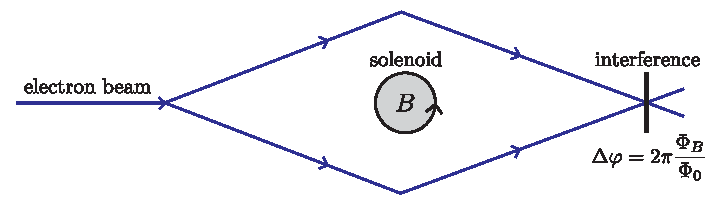
\includegraphics[]{Figures/Chapter7/aharonov_bohm.pdf}
\caption[The Aharonov-Bohm experiment]{The Aharonov-Bohm experiment. A coherent electron beam is split into two paths surrounding a solenoid which produces a non-zero magnetic field $\mathbf{B}$ inside the gray region and $\mathbf{B}=0$ outside. The two beams are later recombined and an interference pastern reveals a phase difference $\Delta\varphi = 2\pi \Phi_B/\Phi_0$ equal to the magnetic flux enclosed by the electron's path.}
\label{fig:aharonov_bohm}
\end{center}
\end{figure*}

This Aharonov-Bohm phase can be interpreted as an example of a Berry phase in real space. For a charged particle in the presence of a vector potential the momentum dependence of the free-particle Hamiltonian is modified $\mathbf{p}\rightarrow\mathbf{p}-q\mathbf{A}$ so that the wave function will depend on the magnetic vector potential as well. Using Equations~\ref{eq:berry_phase} and~\ref{eq:berry_connection} it can be shown that the Berry phase associated to a closed path around the solenoid is exactly equal to the Aharonov-Bohm phase: 
%
\begin{align}
	\gamma_n(\mathcal{C})=&\frac{e}{\hbar}\oint_{\mathcal{C}}\mathbf{A}(\mathbf{r})\cdot d\mathbf{r} \nonumber \\
	=& \frac{e}{\hbar}\int_{\mathcal{S}}\nabla\times\mathbf{A}\cdot d\mathbf{S} \nonumber \\
	=& \frac{e\Phi_B}{\hbar},
	\label{eq:aharonov_bohm_phase}
\end{align}

For this particular example, the Berry connection is exactly equal to the magnetic vector potential and the Berry curvature is the magnetic field. This gives us a very physical intuition for interpreting the Berry phase in terms of the `magnetic flux' from abstract sources of `magnetic fields' in parameter space.  

\subsection{Chern number}

The Chern number is conventionally used to describe the topology of materials which have an underlying crystalline structure. According to Bloch's theorem, the wave functions of a space periodic Hamiltonian can be written as $\ket{\psi(\k)}=e^{i\k\cdot\mathbf{r}}\ket{u(\k)}$, where $\ket{u(\k)}$ are periodic wave functions. If we define the Bloch Hamiltonian
%
\begin{equation}
	\hat{H}(\k)=e^{i\k\cdot\mathbf{r}}\hat{H}(\mathbf{r})e^{-i\k\cdot\mathbf{r}}, 
\end{equation}
%
their eigenvectors are given by $\ket{u(\k)}$ and the eigenvalues define the band structure. Translational symmetry implies that $\hat{H}(\k+\mathbf{a})=\hat{H}(\k)$ where $\mathbf{a}$ is a reciprocal lattice vector. The crystal momentum or quasimomentum is only defined within the periodic Brillouin zone and therefore can be mapped into a torus in $d$ dimensions if we glue the edges together.  

The Chern number of the $n$th band is defined as
%
\begin{equation}
	C_n=\frac{1}{2\pi}\int_{BZ}\mathbf{\Omega}_n d\k,
	\label{eq:chern_number}
\end{equation}
%
where the relevant parameter space is crystal momentum and the surface of integration corresponds to the BZ (a torus). The definition of Chern number is closely related to the definition of the Berry phase from Equation~\ref{eq:berry_connection}. For our previous example of a quantum Hall system, the integer proportionality factor in the quantized conductance is exactly equal to the Chern number. 

Just like two-dimensional surfaces are classified by the integral of their Gaussian curvature, the topology of Bloch bands and of quantum systems in general is determined by the integral of the Berry curvature. In a similar way, the integral connects local properties of a quantum system, the Berry connection, with a global topological invariant, the Chern number. One subtle difference is that the Euler characteristic is only determined by the surface (and its intrinsic Gaussian curvature) while the Chern number is defined both by a surface (the BZ) and an additional local curvature (the Berry curvature). By studying different Hamiltonians one can obtain a different Berry curvature, but the geometry of the BZ and thereby the surface of integration is typically defined by a torus\footnote{In next chapter we consider a case where this breaks down.}. This difference will be important later on when we describe the experiments performed to study a system with Rashba spin-orbit coupling and an unconventional topology. %Using our intuition from the Aharonov-Bohm phase, the Chern number can also be interpreted as the total flux from a `Berry field'  defined in the BZ and whose sources are `monopoles' given by degeneracies in the Hamiltonian. 

% Even though the Chern invariant was initially conceived to classify the topology of systems in momentum space, there have been experiments that studied the topology of quantum systems in other abstract parameter spaces, see for example ~\cite{roushan_observation_2014} and \cite{sugawa_second_2018}.

\section{The bulk-edge correspondence principle}

Earlier I mentioned that topological systems provide very robust channels for transporting things like electrical current and light. This transport phenomena typically arises when there is a spatial interface between two topologically distinct phases. The electrons skipping orbits at the interface of a (topological) quantum Hall material and (trivial) vacuum are one example of this. Notice that for this particular example the modes propagate along a given direction, they are chiral. In general one can expect to have modes moving along two directions, and the difference between the number of these modes $N_L - N_R$ is fixed and determined by the topology of the bulk states. The bulk-edge correspondence principle relates the difference in the number of these modes with the bulk topology of the materials at the interface:
%
\begin{equation}
	\Delta C=N_R - N_L
\end{equation}
%
where $\Delta C$ is the difference of Chern number on the interface. 

\section{Example: two-level model}
\label{sec:2_level_topology}

Many of the concepts introduced in the previous section can be readily applied and understood using a two-level model
%
\begin{equation}
	\hat{H}(\mathbf{k})= \mathbf{h}(\mathbf{k})\cdot\hat{\boldsymbol{\sigma}}
	\label{eq:2D_Hamiltonian}
\end{equation}
%
where $\hat{\boldsymbol{\sigma}}=(\sigma_x, \sigma_y, \sigma_z)$ are the Pauli matrices and $\mathbf{h}(\mathbf{k})=(h_x(\k),h_y(\k), h_z(\k))$ are functions of $\k$. This model has been used to describe a number of physical systems like graphene~\cite{haldane_model_1988} and spin-orbit coupled systems~\cite{bychkov_oscillatory_1984,dresselhaus_spin-orbit_1955}. Let us now consider the simple case $h(\k)=\k$, for which $\nabla_{\k}\hat{H}=\boldsymbol{\sigma}$ and using Equation~\ref{eq:alternative_berry_con} it can be shown that
%
\begin{equation}
	\mathbf{\Omega}=-\frac{\mathbf{h}}{2h^3}
	\label{eq:monopole}
\end{equation}
%
which can be recognized as the field of a Dirac monopole~\cite{dirac_paul_adrien_maurice_quantised_1931} with charge $-1/2$. The degeneracy in the energies that gives rise to the monopole is known as a Dirac point as the energies in that vicinity resemble the dispersion of a massless Dirac particle. It follows from Equation~\ref{eq:monopole} that the Berry phase gained by moving in a closed path $\mathcal{C}$ is equal to the flux from the monopole in the surface enclosed by $\mathcal{C}$ as is shown in Figure~\ref{fig:solid_angle}. This connects nicely with our intuition from the Aharonov-Bohm effect. For a closed surface enclosing the Dirac point, the Chern number is an integer equal to 1. 
%
\begin{figure*}[htb]
\begin{center}
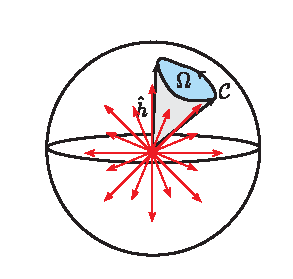
\includegraphics[]{Figures/Chapter7/solid_angle.pdf}
\caption[Graphical representation of Chern number]{For a two-level system, the Berry curvature from a Dirac point can be viewed as a Dirac monopole in momentum (parameter) space. The Chern number can be interpreted as the flux from the monopole on the solid angle subtended by the vector $\hat{h}(\k)$ or alternatively as the number of times $\hat{h}(\k)$ wraps around a unit sphere.}
\label{fig:solid_angle}
\end{center}
\end{figure*}

For a Hamiltonian with arbitrary $\mathbf{h}(\k)$ we can define a normalized vector $\hat{h}=\mathbf{h}/\vert\mathbf{h}\vert$ and the Chern number takes the form
%
\begin{equation}
	C=\frac{1}{4\pi}\int(\partial_{k_x}\hat{h}\times\partial_{k_y}\hat{h})\cdot\hat{h} \, d\k
\end{equation}
%
and can be interpreted as the number of times that the vector $\hat{h}(\k)$ wraps around a unit sphere~\cite{kaufmann_notes_2016}, a quantity that is known as the winding number.

% \note{My current points of confusion are the following:}
% Why is the Chern number for a single Dirac point on a torus a half? I'm thinking in particular for the quantum hall effect and the example on section 2 on the review on topological insulators. Also how to go from closed paths in parameter space to closed surface integrals?
% Also keep in mind Krammers theorem: for every energy eigenstate of a time-reversal symmetric system with half-integer total spin, there is at least one more eigenstate with the same energy. In other words, every energy level is at least doubly degenerate if it has half-integer spin.
% Why is $h_z\neq0$ the same as breaking time reversal symmetry? What about the other components? 

\section{Monopoles and Dirac strings}

We just gained some intuition about interpreting the Chern number as the flux from Dirac monopoles. But if we stick to our knowledge of electromagnetism we might remember that monopoles are forbidden since
%
\begin{equation}
	\int_{\mathcal{S}}\mathbf{B}\cdot d\mathbf{S}=\int_{V}(\nabla\cdot\mathbf{B})dV
\end{equation}
%
and $\nabla\cdot\mathbf{B}=\nabla\cdot(\nabla\times\mathbf{A})=0$. So how is this possible? The solution to this problem was envisioned by Dirac~\cite{dirac_paul_adrien_maurice_quantised_1931} and is now called a Dirac string. If we consider an semi-infinitely long and infinitesimally thin solenoid, the magnetic field in the finite end will resemble that of a monopole as can be seen in Figure~\ref{fig:monopole}. This tiny solenoid corresponds to the Dirac string. 
%
\begin{figure*}[htb]
\begin{center}
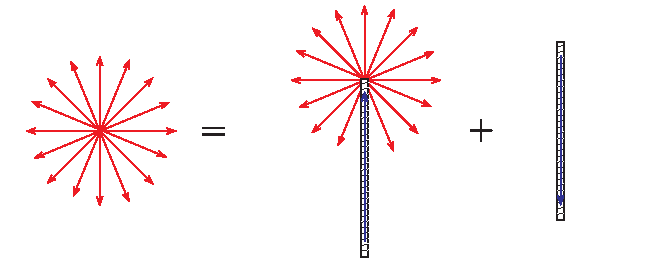
\includegraphics[]{Figures/Chapter7/monopole.pdf}
\caption[Graphical representation of Chern number]{For a two-level system, the Berry curvature from a Dirac point can be viewed as a Dirac monopole in momentum (parameter) space. The Chern number can be interpreted as the flux from the monopole on the solid angle subtended by the vector $\hat{h}(\k)$ or alternatively as the number of times $\hat{h}(\k)$ wraps around a unit sphere.}
\label{fig:monopole}
\end{center}
\end{figure*}
A more mathematical interpretation of these strings comes from the fact that the vector potential of a monopole has `lines' where it becomes singular. For example for a particular gauge we can write
%
\begin{equation}
	\mathbf{A}(\r)=g\frac{-y\ex+x\ey}{r(r+z)}
\end{equation}
%
which is singular for the negative $z$ axis where $z=-r$. The orientation of the Dirac string is gauge dependent, something that should not surprise or bother us at this point. However, the physical effects of the Dirac string should be gauge independent, or in other words, the Aharonov-Bohm phase gained by a charged particle moving in a path that encloses the string should be an integer multiple of $2\pi$. This is argument gives rise to the Dirac charge quantization~\cite{dirac_paul_adrien_maurice_quantised_1931}, and in the context of topology, it guarantees that when we calculate the Berry phase by integrating the Berry connection (vector field) along a path that enclose a Dirac string, its effect will be indistinguishable. 


% In order for the field resulting from this string to be indistinguishable from that of a monopole, the Aharonov-Bohm phase gained by an electron moving around it has to be indistinguishable. For a monopole with charge $g$ this means that $2\pi N=\Phi_g/\Phi_0$

% A For this gauge choice, the $-z$ axis corresponds to the Dirac string. The orientation of the string might change for a different basis but if we demand that the field resulting from either of this vector potentials 


% I mentioned earlier that the Berry curvature from a Dirac point looks like a monopole and that the flux from this monopole on a closed surface is equal to the Chern number. This 
% If we try to write the vector potential for a monopole we will find that there is a line where it becomes singular. For example, for a monopole with charge g we can write
% %
% \begin{equation}
% 	\mathbf{A}(\r)=g\frac{-y\ex+x\ey}{r(r+z)}
% \end{equation}
% %
% which is singular at the south pole where $z=-r$. We could alternatively write 
% %
% \begin{equation}
% 	\mathbf{A}(\r)=g\frac{y\ex-x\ey}{r(r-z)}
% \end{equation}
% %
% which leads to the same 
% The existence of Dirac monopoles comes with some interesting consequences. A magnetic monopole can be thought of as the end of a semi-infinitely long and infinitesimally thin magnetic solenoid. In order for the field of the solenoid to be indistinguishable from that of a monopole, the Aharonov-Bohm phase gained by an electron moving around it has to be indistinguishable. For a monopole with charge $g$ this means that $2\pi N=\Phi_g/\Phi_0$

% . This thin solenoid can in fact be identified with  


% The existence of Dirac monopoles means that there has to be a singularity in the vector potential. 


% to be a Dirac string~\cite{dirac_paul_adrien_maurice_quantised_1931}. Dirac envisioned having an infinitesimally thin solenoid whose end looks like a magnetic charge. The monopole can only be identified as such if the thin solenoid is not experimentally detectable.

% Lets imagine for a moment 
% %
% \begin{equation}
% 	\int_{\mathcal{S}}\mathbf{B}\cdot d\mathbf{S}=q_m
% \end{equation}

% It is possible to find a magnetic vector potential 
% m This objects were conceived by Dirac as tiny solenoids
% If magnetic monopoles exist then electric charge must be quantized
% In electromagnetic theory 

% A consequence of the Berry connection being singular 

% This vector potential has one problem. It is singular at the north pole (z = r). In fact, one can prove that no matter which gauge one uses, there will always be a singularity point.

% Degeneracies as sources of Berry curvature field. There must therefore be Dirac strings as well...

\section{Conclusions}

Topology plays a very important role both in math and in physics. In this Chapter I reviewed the basic concepts of topology in the context of condensed matter physics that will be relevant for our experiments with unconventional topology. As a closing remark, Figure~\ref{fig:topology_analogies} summarizes the main concepts that were introduced and is a reminder that topological invariants are global properties defined in terms of integrals of local properties. Furthermore, we can use our intuition from electromagnetic theory to interpret topological invariants in quantum mechanics. 

 \begin{figure*}[htb]
\begin{center}
\includegraphics[]{Figures/Chapter7/topology_analogies.pdf}
\caption[Different topological invariants]{The Euler characteristic and the Chern number are topological invariants defined by integrals of local curvatures. The Aharonov-Bohm phase gives us physical intuition to interpret the Chern number as the flux from a `Berry field'.}
\label{fig:topology_analogies}
\end{center}
\end{figure*}

%%%%%%%%%%%%%%%%%%%%%%%%%%%%%%%%%%%%%%%%%%%%%%%%%%%%%%%%%%%%%%%
%
%Graveyard
%
%%%%%%%%%%%%%%%%%%%%%%%%%%%%%%%%%%%%%%%%%%%%%%%%%%%%%%%%%%%%%%%%


% If there is inversion ($\mathcal{P}$) and time reversal ($\mathcal{T}$) symmetry $h_z(\k)=0$ and there are points where the Hamiltonian in Equation~\ref{eq:2D_Hamiltonian} becomes singular. For example, in graphene this occurs in two points. In the vicinity of these points $\q=\k-\k_0$, Equation~\ref{eq:2D_Hamiltonian} resembles the Hamiltonian of a massles Dirac fermion $\hat H(\mathbf k)=\hbar v_F\mathbf q\cdot \vec \sigma$, where $v_F$ is a velocity. 
 
% The $\mathcal{T}$ symmetry can be broken for example by applying a magnetic field, in which case the degeneracy at the Dirac point is broken and \ref{eq:2D_Hamiltonian} becomes a massive Dirac Hamiltonian. 


%  For simplicity lets consider $\mathbf{h}(\k)=h(\sin\theta\cos\phi,\sin\theta\sin\phi,\cos\theta)$. The Hamiltonian has eigenvalues $\pm h$ and the eigenstates are
% %
% \begin{align}
% 	\ket{+}=&(\sin\theta/2e^{-i\phi}, -\cos\theta/2 )  \nonumber \\
% 	\ket{-}=&(\cos\theta/2e^{-i\phi}, \sin\theta/2) 
% \end{align}
%

%For a small and constant value of $h_z$, $\hat{h}$ only wraps around the top or lower half of the Bloch sphere, depending on the sign of $h_z$.

% If $h_z=0$ there are Dirac points\footnote{This can happen if there is inversion ($\mathcal{P}$) and time reversal ($\mathcal{T}$) symmetry} where $\vert\mathbf{h}\vert=0$ and near these ponits Equation~\ref{eq:2D_Hamiltonian} locally resembles the Hamiltonian of a massless Dirac fermion. Near the Dirac points the Berry connection can be written as

			% !TEX root = mainthesis.tex
%Chapter 8

\renewcommand{\thechapter}{8}

\chapter{Unconventional topology with a Rashba SOC quantum gas}
\label{ch:Rashba}

There has been considerable interest in engineering non-Abelian gauge potentials in ultracold atomic systems~\cite{wilczek_appearance_1984,ruseckas_non-abelian_2005}. In particular, Rashba-type~\cite{bychkov_oscillatory_1984}, an example of a non-Abelian gauge potential, has multiply degenerate single particle eigenstates which could open the possibility of studying strongly correlated phases in the presence of interactions for systems of both fermions and bosons~\cite{stanescu_spin-orbit_2008,sedrakyan_composite_2012,hu_probing_2011}. However, in order to observe meaningful many-body physics it is necessary to have a long lived system and even though 2D SOC has been previously realized in ultracold $^{40}$K\cite{huang_experimental_2016} the experiments were limited by the collisional relaxation lifetime due to the coupling of atoms in different hyperfine manifolds. These concerns motivated a new proposal~\cite{campbell_rashba_2016} to engineer Rashba SOC within the ground hyperfine manifold of alkali atoms using the RF dressed $\xyz$ states discussed in Chapter~\ref{ch:clock_states} and Raman transitions. 

Even though this new proposal offered many advantages compared to previous experiments, we were still feeling very pessimistic about the lifetime of our system mostly because of spontaneous emission from the Raman lasers. Rather than trying to measure a fragile many-body phase we decided to instead shift our focus into topology as the Rashba Hamiltonian has a topologically non-trivial dispersion relation. Unlike conventional materials, there is no underlying crystalline structure leading to Chern numbers that can take unconventional half-integer values. 

Ultracold atomic systems are an emerging platform for engineering topological lattices, from the Harper-Hofsdater model\cite{miyake_realizing_2013,aidelsburger_realization_2013}, the Haldane model\cite{jotzu_experimental_2014}, to the Rice-Mele model\cite{lu_geometrical_2016,lohse_thouless_2016} as well as assembling spin-orbit coupled lattices without analogues in existing materials\cite{wu_realization_2016,sun_highly_2018}. 

Experimental realizations of topological materials have focused on engineering different topological bands (with different Berry curvatures) in lattice systems, where the BZ is always a torus. We show that by eliminating the lattice potential and thereby changing  the BZ from ${\mathbb T}^2$ to ${\mathbb R}^2$, i.e. from a torus to a Cartesian plane, it is possible to create topological branches of the dispersion relation with half-integer Chern number. In our experiments we created both topological and non-topological dispersion branches by introducing Rashba-like spin-orbit coupling (SOC)\cite{campbell_realistic_2011, huang_experimental_2016, meng_experimental_2016} to a cold quantum gas. 

In this Chapter I will describe a series of experiments that we performed to engineer and characterize the topology of a Rashba spin-orbit coupled quantum gas. First I describe the engineering of the Rashba Hamiltonian using a trio of Raman coupled CDD states (Chapter~\ref{ch:clock_states}) and validate our quantum engineering using Fourier transform spectroscopy (Chapter~\ref{ch:Fourier_spectroscopy}).  Then I will describe a quantum state tomography procedure to measure the eigenstates of our system, and directly obtain the Chern number for both a topologically trivial and non-trivial configuration, where it respectively takes the value of zero or a half integer. To avoid confusion between dressed state $xyz$ labels and Cartesian coordinates, in this Chapter I will use the numbers $1,2,3$ to label the coordinates $\ex, \ey, \ez$ and the letters $x,y,z$ to label dressed state parameters. 

\section{Rashba spin-orbit coupling}

Rashba SOC~\cite{bychkov_oscillatory_1984} appears in condensed matter systems where electrons are confined in a 2D plane and experience an intrinsic out-of-plane electric field. If the electron's momentum is given by $\hbar\k=\hbar(k_x\ex+k_y\ey)$ and the electric field is $\mathbf{E}=E\ez$, in the electron's moving frame there will be a momentum dependent magnetic field $\mathbf{B}_{\rm SOC}=-\hbar\k/m\times\mathbf{E}/c^2=\hbar E/mc^2(-k_y, k_x, 0)$. The interaction between the electron's spin with this field through the magnetic Zeeman interaction $-\mathbf{\mu}\cdot{\mathbf{B}_{\rm SOC}}$ gives rise to the SOC Hamiltonian
%
\begin{equation}
	\hat{H}_{\rm SOC}=\frac{2\alpha}{m}(k_y\hat{\sigma}_x-k_x\hat{\sigma}_y)
	\label{eq:Rashba_ham}
\end{equation}
%
where $\alpha=g\mu_BE/c^2$, $g$ is the electrons gyromagnetic ratio, $\mu_B$ is the Bohr magneton and $\hat{\sigma}_i$ are the Pauli matrices. 

The Rashba dispersion relation is characterized by having a Dirac point located at $\k=0$ (see Chapter~\ref{sec:2_level_topology}) and a degenerate ground state that is described by the ring $k_x^2+k_y^2=\alpha^2$. \note{TODO: Make figure} If we combine Equation~\ref{eq:Rashba_ham} with the free particle Hamiltonian the Hamiltonian can can be written as $\hat{H}=(\hbar\k-\hat{\mathbf{A}})^2/2m$ where $\mathbf{\hat{A}}=\alpha(\hat{\sigma}_y\ex-\hat{\sigma}_x\ey)$ can be interpreted as a (matrix valued) non-abelian gauge potential whose elements do not commute. This term is closely related to the Berry connection discussed in Chapter~\ref{sec:Berry phase and curvature}. This in combination with the presence of the Dirac point hints to us that a system with Rashba SOC has non-trivial topology. 

SOC is also a necessary ingredient for realizing $\mathds{Z}_2$ topological insulators and the quantum spin-Hall effect. Furthermore, the degeneracy of the ground state single particle eigenstates could open the possibility of studying strongly correlated phases in the presence of interactions for systems of both fermions and bosons~\cite{stanescu_spin-orbit_2008,sedrakyan_composite_2012,hu_probing_2011}. SOC systems offer the possibility of studying a wide range of interesting physics and naturally using ultracold atomic systems to engineer SOC, and in particular Rashba type SOC, has been a longstanding goal~\cite{galitski_spin-orbit_2013}. 


\section{Rashba SOC for neutral atoms}
\label{sec:rashba_ring_coupling}

Proposals for engineering Rashba type SOC in neutral atoms consist in using lasers to link internal states of an atom with its linear momentum. In order to achieve non-trivial gauge potentials it is necessary to couple $N\geq3$ levels (see~\cite{goldman_light-induced_2014}). I will describe the proposal by~\cite{campbell_realistic_2011} which considers a `ring coupling' which is shown in Figure~\ref{fig:rashba_ring_coupling} for the case of $N=3$. The states $\ket{j}$ represent internal atomic states and they are linked to each other with complex valued matrix elements $\frac{\Omega_j}{2}e^{i\k_{j}\cdot\x}$, where $\k_{j}$ is a momentum transfer associated with the $\ket{j}\rightarrow\ket{j+1}$ transition and $\Omega_i=e^{i\phi_i}\vert\Omega\vert$ represents the coupling strength. We require that $\sum\k_i=0$ so that no momentum is transfered when a closed loop $\ket{1}\rightarrow\ket{2}\dots \rightarrow\ket{N}\rightarrow\ket{1}$ is completed. For this case the $\k_i$ momenta vectors can be written as $\k_j=\mathbf{K}_{j+1}-\mathbf{K}_j$, and we make $\mathbf{K}_j=\kl\sin(2\pi j/N)\ex+\kl\cos(2\pi j /N)\ey$, corresponding to the vertices of an N sided regular polygon. We can further make a gauge transformation such that we can replace the phases $\phi_i$ associated to each coupling with $\bar{\phi}=\sum_i\phi_i/N$.

\begin{figure*}[htb]
\begin{center}
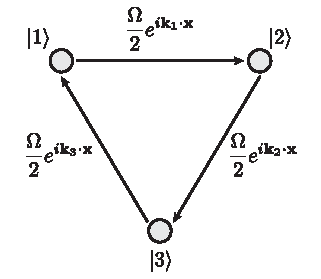
\includegraphics[]{Figures/Chapter8/Rashba_ring_coupling.pdf}
\caption[The Rashba ring coupling]{The Rashba ring coupling. To generate Rashba SOC in a system of cold atoms it is necessary to cyclically couple $N\geq3$ internal states such that the transition $\ket{j}\rightarrow\ket{j+}1$ has a momentum transfer $\k_j$ and $\sum_j\k_j=0$ such that there is no momentum transfer for a closed loop $\ket{1}\rightarrow\ket{2}\dots\ket{N}\rightarrow\ket{1}$. The ring coupling combined with the free particle Hamiltonian give rise to a 2-level subspace that can be described to first order by the Rashba Hamiltonian}
%
\label{fig:rashba_ring_coupling}
\end{center}
\end{figure*}
%
The Hamiltonian describing this coupling along with the kinetic term is 
%
\begin{equation}
	H_{j, j'}=\frac{\hbar^2 k^2}{2m}\delta_{j,j'} + \frac{\Omega}{2}(e^{i(\bar{\phi}+\k_j\cdot\x)}\delta_{j, j'+ 1} + {\rm h.c.}),
\end{equation}
%
and after applying the unitary transformation $U_{j, j'}=\exp[i\mathbf{K}_i\cdot\x]\delta_{j,j'}$\footnote{This transformation is equivalent to applying a state dependent momentum boost $\k\rightarrow \k +\mathbf{K}_j $} it gets transformed to 
%
\begin{equation}
	H_{j,j'}=\frac{\hbar^2}{2m}\vert \q +\mathbf{K}_j\vert^2\delta_{j,j'} + \frac{\Omega}{2}(e^{i\bar{\phi}}\delta_{j, j'+ 1} + {\rm h.c.}),
	\label{eq:rashba_tight_binding}
\end{equation}
%
where I have replaced the momentum $\k$ by the quasimomentum $\q$. The off diagonal terms of Equation~\ref{eq:rashba_tight_binding} can be related to a 1D periodic tight-binding Hamiltonian with hopping elements $\Omega/2$ where the internal states $\ket{j}$ represent lattice sites and completing one loop corresponds to gaining a `flux' of $N\bar{\phi}$. It is helpful to write the Hamiltonian in a basis that is conjugate to the index $j$
%
\begin{equation}
	\ket{l}=\frac{1}{\sqrt{N}}\sum_{j=1}^N e^{i2\pi jl/N}\ket{j}
\end{equation}
%
where the index $l$ is analogous to the crystal momentum index for a Bloch Hamiltonian. In this new basis, terms with oscillatory components (e.g. $\vert \q + \mathbf{K}_j\vert$) in the diagonals are displaced to the off-diagonal and oscillatory terms in the off diagonal are displaced to the diagonal. Under this basis the Hamiltonian starts looking very much Rashba-like
%
\begin{equation}
	H_{l,l'} = \left[\frac{\hbar^2}{2m}(q^2+ k_L^2)+E_l\right]\delta_{l,l'} + \frac{\hbar^2\kl}{m}\left[(iq_x+q_y)\delta_{l-1,l'}+{\rm h.c}\right],
	\label{eq:ring_coupling_ft}
\end{equation}
%
where $E_L=2\hbar\Omega\cos(2\pi l/3+\bar{\phi})$ correspond to the eigenenergies when $q=0$. The phase $\bar{\phi}$ can be tuned such that a pair of states with consecutive $l$ index become degenerate, indicating the presence of a Dirac point at $q=0$. Figure~\ref{fig:ring_coupling_energies} shows the energies $E_l$ for $N=3$ and $\bar{\phi}=0$.

\begin{figure*}[htb]
\begin{center}
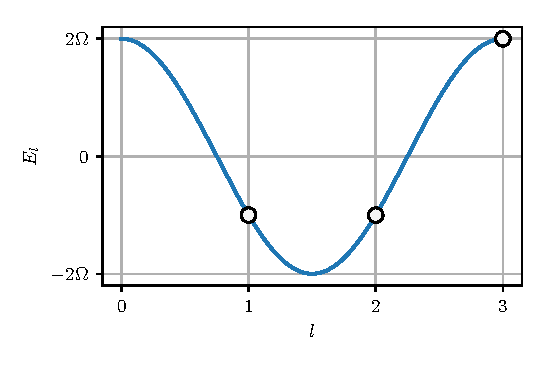
\includegraphics[]{Figures/Chapter8/ring_coupling_energies.pdf}
\caption[Rashba ring coupling eigenenergies]{Eigenenergies of Equation~\ref{eq:ring_coupling_ft} for $q=0$ for $N=3$ and $\bar{\phi}=0$. For this particular choice of phase, the energies of the $l=1$ and $l=2$ states become degenerate}
\label{fig:ring_coupling_energies}
\end{center}
\end{figure*}

We consider the degenerate states corresponding to two consecutive $\ket{l}$ states as pseudospins which are described to zeroth order by the Rashba plus free particle Hamiltonian
%
\begin{equation}
	\hat{H}^{(0)} = \frac{\hbar^2q^2}{2m} + \frac{\hbar^2\kl}{m}(\hat{\sigma_x}q_y-\hat{\sigma}_yq_x), 
\end{equation}
 %
with spin orbit coupling strength given by $\alpha=\hbar^2k_L/2$. The zeroth-order Hamiltonian has continuous rotational symmetry while we the proposed ring coupling only has only discrete rotational symmetry. The symmetry of the Hamiltonian is recovered when higher order corrections of the Hamiltonian are included. The complete expressions for the higher order terms for $N=3$ and $N=4$ can be found in~\cite{campbell_realistic_2011}, and they are reminiscent of quadratic and cubic Dresselhaus SOC~\cite{stanescu_spin_2007}. The largest leading order term is inversely proportional to $\Omega^2$ so that this ring-coupling scheme results in a more `Rashba-like' Hamiltonian as one goes to higher coupling strengths. Figure~\ref{fig:rashba_alien} shows level curves of the ground state eigenenergies of Equation~\ref{eq:ring_coupling_ft} for $N=3$ and $\bar{\phi}=0$ for increasing $\Omega$. At low $\Omega$ the dispersion has discrete rotational symmetry and is characterized by three local minima. As $\Omega$ is increased the local minima start merging into each other and in the large $\Omega$ limit we recover the characteristic Rashba ring-like dispersion.   

\begin{figure*}[htb]
\begin{center}
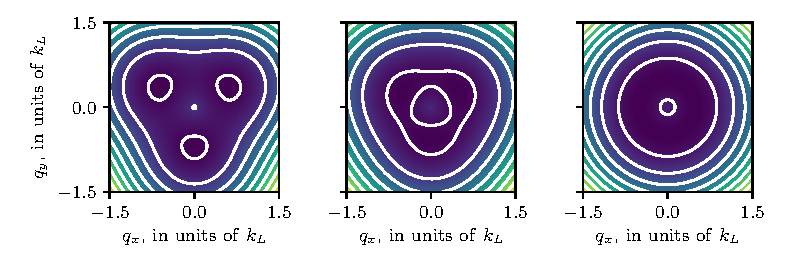
\includegraphics[]{Figures/Chapter8/rashba_alien.pdf}
\caption[Rashba ring coupling ground state dispersion]{Ground state dispersion relation of Equation~\ref{eq:ring_coupling_ft} for $N=3$ and $\bar{\phi}=0$ for $\Omega=\unit[1.75]{\El}$ (left), $\Omega=\unit[3.5]{\El}$ (middle) and $\Omega=\unit[175]{\El}$ (right). Higher order corrections to $\hat{H}^{(0)}$ decay as $1/\Omega^2$ and in the large $\Omega$ limit we recover the Rashba ring dispersion.}
\label{fig:rashba_alien}
\end{center}
\end{figure*}

So far we have only considered the case where all the coupling strengths and the vectors $\k_j$ are symmetric. In the lab it might be hard due to constraints imposed by the capabilities of an experimental apparatus. As one departs from the ideal ring-coupling, we find that the resulting dispersion can looses its discrete rotational symmetry. While this perturbations can have a significant impact on the dispersion, the Dirac point is remarkably robust and as long as $\bar{\phi}$ is such that there are at least two degenerate states in the ideal ring coupling case the Dirac point will remain gapless although it might move from $\q=0$. The exact location of the Dirac point as a function of $\Omega_i$ and $\q$ for an imperfect ring-coupling scheme is derived in \cite{huang_experimental_2016}. Figure~\ref{fig:rashba_perturbed} shows some examples of how the ground state dispersion is modified when the vectors $\mathbf{K}_j$ that don't lie in the vertices of a regular polygon and when the amplitude of $\Omega$ is state dependent. 

\begin{figure*}[htb]
\begin{center}
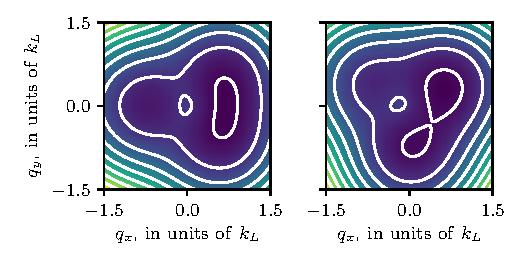
\includegraphics[]{Figures/Chapter8/rashba_perturbed.pdf}
\caption[Perturbed Rashba dispersion]{(left) Ground state dispersion relation of Equation~\ref{eq:ring_coupling_ft} for $N=3$ and $\bar{\phi}=0$ for $\Omega=\unit[1.75]{\El}$ but $\mathbf{K}_j$ that don't correspond to to the vertices of an isosceles triangle rather than an equilateral triangle. Ground state dispersion for symmetric $\mathbf{K}_j$ but state dependent $\Omega=$. In both cases the discrete rotational symmetry is lost but the gapless Dirac point remains.}
\label{fig:rashba_perturbed}
\end{center}
\end{figure*}

\section{Experimental implementation of Rashba SOC}

 We implemented the ring-coupling scheme and thereby engineered Rashba SOC by resonantly coupling three internal atomic states using two-photon Raman transitions\cite{campbell_rashba_2016} as depicted in Figure~\ref{fig:Schematic}. As shown in Figure~\ref{fig:Schematic}a, the engineered system consisted of an effective spin-1/2 Rashba subspace, along with a topologically trivial high-energy branch. Our engineered Rashba system had a single Dirac cone near $\q=0$, where the two lower dispersion branches become degenerate and the Berry curvature becomes singular. Each of these branches extend to infinite momentum, making the supporting manifold a plane rather than a torus. We characterized this system using both spectroscopy and quantum state tomography. This allowed us to measure the dispersion branches and directly observe the single Dirac point linking the lowest two branches as well as to reconstruct the Berry connection to derive the associated Chern numbers. \note{TODO:maybe the stuff of plane and torus doesn't go here}


%%%%%%%%%%%%%%%%%%%%%%%%%%%%%%%%%%%%%%%%%%%%%%%%%%%%%%%%%%%%%%%%%%
%
% Brief descrpiption of Rashba SOC: theory and implementation
%
%%%%%%%%%%%%%%%%%%%%%%%%%%%%%%%%%%%%%%%%%%%%%%%%%%%%%%%%%%%%%%%%%%

\begin{figure*}[htb]
\begin{center}
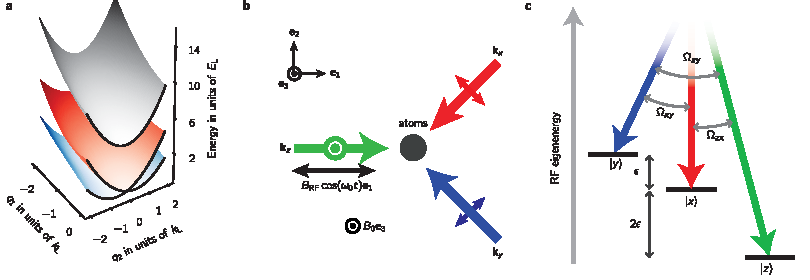
\includegraphics[width=\textwidth]{Figures/Chapter8/fig1.pdf}
\caption{{\bfseries a} Our engineered dispersion consisted of a two-level Rashba subspace (red and blue) with a single Dirac point linking the lowest two branches and a topologically trivial higher branch (gray). {\bfseries b} We generated $\xyz$ states by combining a bias magnetic field along $\mathbf{e}_3$ with an RF magnetic field oscillating along $\mathbf{e}_1$. These states were coupled by three cross-polarized Raman laser beams propagating along $\mathbf{e}_1$, $\mathbf{e}_2-\mathbf{e}_1$ and $-\mathbf{e}_1-\mathbf{e}_2$. {\bfseries c} Each pair of Raman lasers was in two-photon resonance with a single transition between the $\xyz$ states which we coupled strengths $(\Omega_{zx}, \Omega_{xy}, \Omega_{yz})/2\pi=\unit[(12.6(5), 8.7(8), 10(1))]{kHz}$.}
\label{fig:Schematic}
\end{center}
\end{figure*}

%%%%%%%%%%%%%%%%%%%%%%%%%%%%%%%%%%%%%%%%%%%%%%%%%%%%%%%%%%%%%%%%%%
%
% Brief details on experimental implementation
%
%%%%%%%%%%%%%%%%%%%%%%%%%%%%%%%%%%%%%%%%%%%%%%%%%%%%%%%%%%%%%%%%%%

All of our experiments started with about with $N\approx 1\times 10^6$$\Rb87$ atoms in a crossed optical dipole trap\cite{lin_rapid_2009}, with frequencies $(f_1,f_2,f_3) \approx \unit[(70, 85, 254)]{Hz}$, just above the transition temperature for Bose-Einstein condensation. We initially prepared the atoms in the $\ket{F=1, m_F=-1}$ state of the $5S_{1/2}$ electronic ground state and transfered atoms to the $m_F=0$ and $m_F=+1$ states as needed using ARP. A bias field $B_0\mathbf{e}_3$ gave a $\omega_0/2\pi=\unit[23.9]{MHz}$ Larmor frequency along with a quadratic shift of $\epsilon/2\pi=\unit[83.24]{kHz}$. The experiments were performed using the $\xyz$ states described in Chapter~\ref{ch:clock_states}. We implemented CDD using an RF magnetic field oscillating at the Larmor frequency with strength $\Omega_{\rm RF}=1.41(2)\epsilon$. We adiabatically prepared the $\xyz$ states starting from the $m_F$ states following the procedure described in Chapter~\ref{sec:xyz_state_preparation}. 

\subsection{Raman coupling the $\xyz$ states}

We Raman-coupled atoms prepared in any of the $\xyz$ states using the three cross-polarized Raman laser beams shown in Figure~\ref{fig:Schematic}b, tuned to the `magic zero' wavelength $\lambda_L = \unit[790]{nm}$. We arranged the Raman lasers into the tripod configuration shown in Figure~\ref{fig:Schematic}c, bringing each pair into two-photon resonance with a single transition with strengths $(\Omega_{zx}, \Omega_{xy}, \Omega_{yz})/2\pi=\unit[(12.6(5), 8.7(8), 10(1))]{kHz}$. The geometry of our experimental implementation differs from~\cite{campbell_rashba_2016} where all Raman lasers are perpendicular. We had to go away from this configuration because we were interested in having all of the Raman recoil vectors lying on the imaging plane so we could image all the Raman induced $\k$ dependent dynamics. As a result of this the dispersion relation no longer has discrete rotational symmetry, however the Dirac point is very robust against changes in Hamiltonian parameters. 

The energies of the $\xyz$ states are $\omega_x=0$ and $\omega_{z,y}=-(\epsilon\pm\sqrt{4\Omega_{\rm RF}^2+\epsilon^2})/2$. We set the frequencies of the Raman lasers to $\omega_x=\omega_L+\omega_0+\omega_{xy}$, $\omega_y=\omega_L+\omega_0$ and $\omega_z=\omega_L-\omega_{zx}$,  where $\omega_L=2\pi c/\lambda_L$ and $(\omega_{zx}, \omega_{xy}, \omega_{zy})/2\pi = \unit[(166.47, 83.24, 249.71)]{kHz}$ are the transition frequencies between pairs of dressed states and are integer multiples of $\epsilon$ for our coupling strength $\Omega = \sqrt{2}\epsilon$. 

The Raman coupled states can be described by the combined kinetic and light-matter Hamiltonian
%
\begin{equation}
	\hat H_{\rm R}(\k) =\sum_{j\in\{xyz\}}\bigg(\frac{\hbar^2k^2}{2m}+\hbar \omega_i\bigg)\ket{j}\bra{j}+\sum_{j'\neq j}\hbar\Omega_{j,j'}e^{i(\k_{j,j'}\cdot\x-i\omega_{j,j'}t)}\ket{j}\bra{j'},
	% \label{Eq:Rashba_atoms}
\end{equation}
%
where $\k_{j,j'}$ is the recoil momentum from an $\ket{j}\rightarrow\ket{j'}$ transition and $\Omega_{ij}$ is the Raman coupling strength between a pair of RF dressed states. The Hamiltonian above only includes the matrix elements associated to resonant couplings. We apply the unitary transformation $\hat{U}_{j,j'}=\exp(-i\k_j\cdot\x-\omega_j t)\delta_{j,j'}\ket{j}\bra{j'}$ so that the Hamiltonian takes the familiar form of the ring coupling scheme
\begin{equation}
	\hat H_{\rm R}=\sum_{j\in\{xyz\}}\bigg(\frac{\hbar^2(\q-\k_j)^2}{2m}+\hbar\delta_j\bigg)\ket{j}\bra{j}+\sum_{j\neq j'}\hbar\Omega_{jj'}\ket{j}\bra{j'},
	\label{Eq:Rashba_atoms}
\end{equation}
%
where $\k_j$ are the Raman wave vectors and $\delta_j$ is the detuning from Raman resonance. 

This coupling scheme simultaneously overcomes three limitations of earlier experiments\cite{huang_experimental_2016,meng_experimental_2016} that performed the ring coupling using a combination of states in the $F=1$ and $F=2$ hyperfine manifolds of $^40$K : (1) working in the same hyperfine manifold eliminates spin-relaxation collisions~\cite{tojo_spin-dependent_2009}; (2) unlike $m_F$ states, the $\xyz$ states can be tripod-coupled with lasers far detuned relative to the excited state hyperfine splitting greatly reducing spontaneous emission\cite{cooper_reaching_2013}; and (3) CDD renders the $\xyz$ states nearly immune to magnetic field noise.
\note{TODO: understand what is the deal with spin-relaxation collisions, also what is the deal with coupling far detuned stuff}

\subsubsection{Floquet and off resonant coupling effects}

We operated in a regime where the transition energies between the $\xyz$ states were integer multiples of $\omega_{xy}$: $\omega_{zx}=2\omega_{xy}$ and $\omega_{zy}=3\omega_{xy}$, and therefore we can use Floquet theory for a complete description of our system\cite{goldman_periodically_2014}. The Hamiltonian in Equation~\ref{Eq:Rashba_atoms} is therefore an effective Hamiltonian that describes the stroboscopic dynamics of the full Floquet Hamiltonian. We observed that the effective Raman coupling strengths for the driven three level system differed from our calibrations which were performed by only driving one pair of states because of the presence of nearby quasi-energy manifolds. This effect could be mitigated for larger values of $\omega_{xy}$ as the spacing between quasi-energy manifolds is increased. Appendix~\ref{app:rashba_derivation} has a full derivation of the Raman Hamiltonian starting from the $\ket{m_F}$ basis in the lab frame including the full time dependence and off resonant terms which can also modify the Hamiltonian parameters. 

\begin{figure*}[htb]
\begin{center}
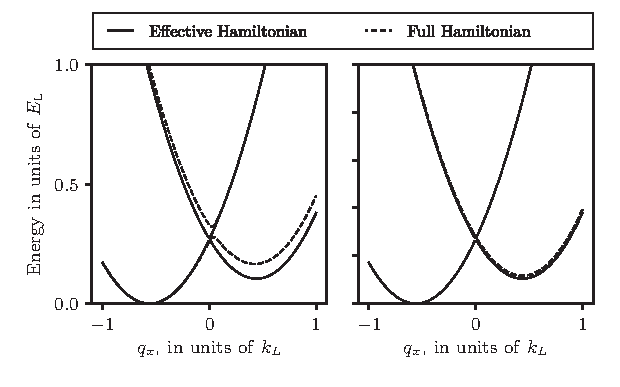
\includegraphics[]{Figures/Chapter8/floquet_effects_legend.pdf}
\caption[Effect of neighboring Floquet manifolds on Rashba dispersion]{Solid lines: Dispersion relation from the effective Floquet Hamiltonian from Equation~\ref{Eq:Rashba_atoms} as a function of $q_x$ for $\Omega_{i,j}=\unit[1.5]{\El}$ and $\delta_i=0$. Dashed lines: Dispersion relation computed for the full Floquet Hamiltonian. We considered $\omega_{zx}=2\omega_{xy}$ and $\omega_{zy}=3\omega_{xy}$ in both cases so the separation between Floquet manifolds is $\omega_{xy}$. In the left panel $\omega_{xy}=\unit[83.24]{kHz}$ as in our experiments and in the right panel $\omega_{xy}=\unit[416.2]{kHz}$. As the spacing between Floquet manifolds becomes larger, the dispersion from the effective and full Hamiltonians become closer.}
\label{fig:floquet_effects}
\end{center}
\end{figure*}

\subsubsection{Lifetime}

The measured spontaneous emission limited lifetime of our system is $\unit[320(17)]{ms}$. However it is reduced to $\unit[40(2)]{ms}$ when the we Raman couple the $\xyz$ states, which we attribute to technical noise in the relative phase between the RF dressing field and the Raman laser fields, which has caused considerable consternation in ongoing experiments. However annoying this reduced lifetime is, all the experiments reported here were short compared to this timescale. Figure~\ref{fig:raman_lifetime} shows measurements of the lifetimes of Raman dressed atoms in both $\ket{m_f}$ and $\xyz$ states. We obtained the lifetime by fitting decaying exponentials to the integrated OD from TOF images of thermal atoms where the Raman was turned on in $\unit[1]{ms}$ and held on for up to $\unit[50]{\mu s}$\footnote{How long we could hold on the Raman was limited by the RF antenna heating up.}. 

\begin{figure*}[htb]
\begin{center}
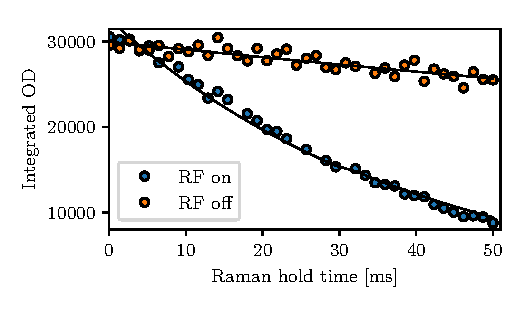
\includegraphics[]{Figures/Chapter8/raman_lifetime.pdf}
\caption[Lifetime of Raman dressed states]{Lifetime of Raman dressed states. We Raman dressed atoms in the $\ket{m_f}$ and $\xyz$ states. The orange markers correspond to atoms initially prepared in $\ket{m_f=-1}$ (no high power RF involved) and the blue markers correspond to atoms $\xyz$ (three averaged traces). The lifetime of doubly dressed states is significantly reduced as compared to the lifetime of the Raman dressed $\ket{m_f}$ states, indicating that of resonant scattering of photons is not our only loss mechanism.}
\label{fig:raman_lifetime}
\end{center}
\end{figure*}

\subsection{Measuring quasimomentum distributions}
Each pair of Raman lasers coupled states $\ket{i, \k}\rightarrow \ket{j, \k+\k_{i,j}}$ where $\ket{i}$ and $\ket{j}$ denote the initial and final $\xyz$ states, $\k$ is the initial momentum and $\k_{i,j}=\k_i-\k_j$ is the two-photon Raman recoil momentum. Dressed states with quasimomentum $\q$ are comprised of three bare states $\ket{j,\k}$ with momentum $\k=\q-\k_j$. The eigenstates of our Rashba SOC Hamiltonian take the form
\begin{equation}
	\ket{\Psi_n(\q)}=\sum_{j\in xyz}\sqrt{a_{n,j}(\q)}e^{i\phi_{n,j}(\q)}\ket{j,\k=\q-\k_{j}},	
	\label{Eq:Raman_wavefunction}
\end{equation}
where the quasimomentum $\q$ is a good quantum number and the amplitudes are parametrized by $a_{n,j}(\q)$ and $\phi_{n,j}(\q)$. We leveraged the wide momentum distribution of a non-condensed ensemble ($T\approx\unit[180]{nK}$ and $T/T_c\approx 1.1$) to sample a wide range of momentum states simultaneously. By starting separately in each of the $\xyz$ states we sampled the range of quasimomentum states shown in Figure~\ref{fig:quasimomentum_map}b, where the momentum distributions of an initial state $\ket{j,\k}$ is shifted from $\q=0$ by the corresponding Raman wave vector $\k_{j}$. 
%
\begin{figure*}[t]
\begin{center}
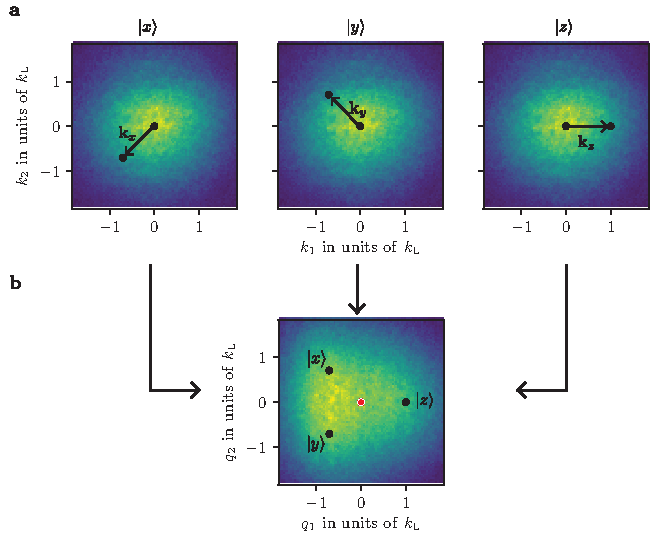
\includegraphics[]{Figures/Chapter8/quasimomentum_map.pdf}
\caption[Mapping momentum into quasimomentum]{Mapping momentum into quasimomentum: {\bf a} We used non-condensed atoms with a broad momentum distribution ($T\approx\unit[180]{nK}$ and $T/T_c\approx 1.1$). {\bf b} Atoms in $\ket{j,\k}$ are mapped to Raman dressed states with quasimomentum $\q=\k+\k_j$. The black dots in the bottom panel represent the location of $\k=0$ for each of the $\xyz$ states and the red dot corresponds to $\q=0$. We performed our experiments starting separately in each of the $\xyz$ states, which allowed us to sample a larger range of quasimomentum states.}
\label{fig:quasimomentum_map}
\end{center}
\end{figure*}

Our measurement protocol consisted of abruptly removing the confining potential and the Raman lasers, initiating a $\unit[21]{ms}$ TOF. During this TOF we adiabatically transformed each of the $\xyz$ states back to a corresponding $\ket{m_F}$ state following the same procedure described in Chapter~\ref{sec:xyz_state_preparation} and spatially separated them using a Stern-Gerlach gradient. Finally we used resonant absorption imaging to measure the resulting density distributions.

The FWHM of the cloud after TOF is about $\unit[700]{\mu m}$ which is much larger than the size of the in-situ cloud $\sim\unit[50]{\mu m}$ and therefore the spatial density distribution of the TOF images represents momentum distribution of the atoms.  For the $\unit[7.4]{\mu m}$ pixel size of our camera and the $3.283$ magnification of our imaging system, the momentum resolution of our images was $\unit[0.018]{\kl}$ and the momentum distributions after TOF had a FWHM of $\sim\unit[2.2]{\kl}$. 

\subsubsection{Correcting shears from gradients}
\begin{figure*}[t]
\begin{center}
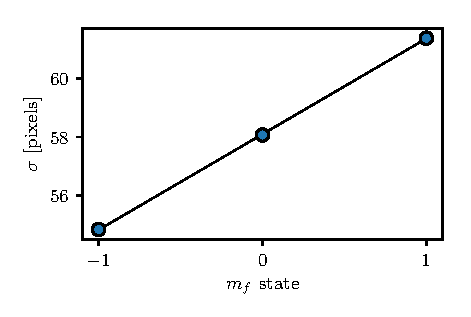
\includegraphics[]{Figures/Chapter8/sg_shear.pdf}
\caption{We measured the standard deviation of the momentum distribution along the axis perpendicular to the SG for 10 shots on each $m_f$ state. From the slope of the linear fit we obtain a shearing parameter $\alpha\approx\pm0.067$ for $m_f=\pm 1$.}
\label{fig:sg_shear}
\end{center}
\end{figure*}

The SG field had a non-zero curvature which caused a compression (or expansion) of the $m_f=-1\ (+1)$ cloud in the direction perpendicular to the SG direction. The projections of a given momentum state $\k$ along the SG axis and perpendicular to it were transformed as $k_{\parallel}\rightarrow k_{\parallel}$ and $k_{\perp}\rightarrow (1+\alpha)k_{\perp}$, where $\alpha=0$ for $m_f=0$ and $\mathrm{sign}(\alpha)=\pm 1$ for $m_f=\pm 1$. Since all our measurements were momentum dependent we had to take special care to quantify and correct this effect on the TOF images. 

We used two different methods to quantify these shears. First we prepared thermal atoms in all three of the $m_f$ states and fit 2D Gaussians rotated by the angle of the SG displacement; $63.8$ degrees for our images. Figure~\ref{fig:sg_shear} shows the standard deviation extracted from the Gaussian fits along the axis perpendicular to the SG deviation as a function of $m_f$ state. We performed a liner fit of $\sigma$ and found that the $m_f=\pm$ states are expanded/contracted by about $\pm 6.7\%$. 

Alternatively we performed the Ramsey interferometer described in Section~\ref{sec:Ramsey} but coupling only 2 states, either $\ket{z}\leftrightarrow\ket{x}$ or $\ket{x}\leftrightarrow\ket{y}$ (mapped to $\ket{-1}\leftrightarrow\ket{0}$ and $\ket{0}\leftrightarrow\ket{+1}$ after TOF). We looked at the oscillation frequencies on each pixel and fit them to Equation~\ref{eq:ramsey_freq} for fixed value of the recoil momentum $\k_{i,j}$ and with a free shear parameter that modifies $\q$. Using this method we extracted a shearing of the order of $7\%$, in good agreement with the Gaussian fitting method.

The transformed momentum coordinates were described by a function $g(\k)=\k^{\mathrm{(shear)}}$ and our observed data $(y_i^{(\mathrm{shear})},\k^{(\mathrm{shear})})$ was the OD in the sheared coordinate system at the $i$th pixel of the CCD sensor. The OD in the unsheared coordinate were estimated using 
%
\begin{equation}
	y_j = \frac{\sum_i\exp[-(g(\k_j)-\k_i^{\mathrm{(shear)}})^2/2\sigma^2]y_i^{\mathrm{(shear)}}}{\sum_i\exp[-(g(\k_j)-\k_i^{\mathrm{(shear)}})^2/2\sigma^2]},
\end{equation}
%
where we used $\sigma$ as the spacing between points in the unsheared coordinate sytem. Prior to any data analysis we applied this transformation to all of our images, where we used different values of $\alpha$ that define $g(\k)$ for each of the $m_f$ states.

\note{TODO: Need to understand origin of this...}
%%%%%%%%%%%%%%%%%%%%%%%%%%%%%%%%%%%%%%%%%%%%%%%%%%%%%%%%%%%%%%%%%%
%
% Results I: Fourier spectroscopy
%
%%%%%%%%%%%%%%%%%%%%%%%%%%%%%%%%%%%%%%%%%%%%%%%%%%%%%%%%%%%%%%%%%

\section{Fourier spectroscopy of the Rashba dispersion}

\begin{figure*}[htb]
\begin{center}
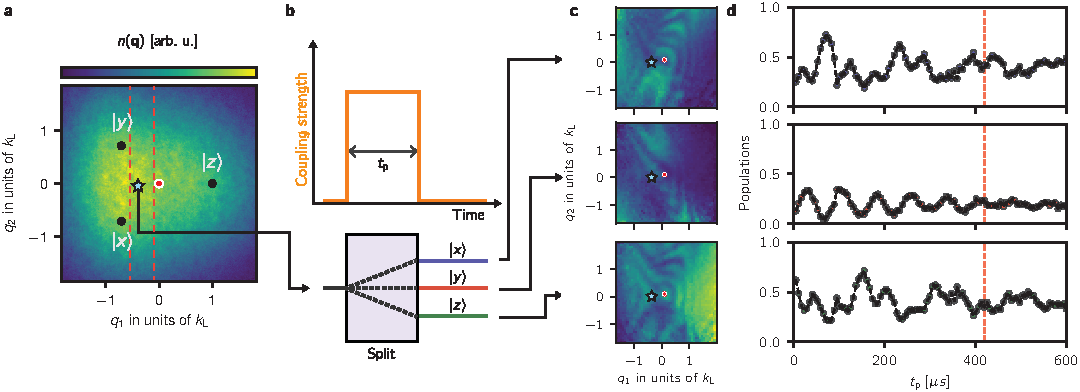
\includegraphics[width=\textwidth]{Figures/Chapter8/fig2.pdf}
\caption{{\bfseries a} Fourier spectroscopy protocol. We applied the Raman lasers for a variable time $t_{\mathrm{p}}$: a Rabi-type atomic interferometer analogous to a three-port beam splitter. {\bfseries b} Probabilities as a function of quasimomentum for a fixed Raman pulse time $t_{\rm p}=\unit[420]{\mu s}$ {\bfseries c} Dynamics of the final populations of the $\xyz$ states with quasimomentum $(q_1, q_2)=\unit[(-0.55,-0.18)]{k_{\rm L}}$ (blue star in panels {\bfseries b}) after initializing the system in the $\ket{z}$ state. }
\label{fig:fourier_spectroscopy}
\end{center}
\end{figure*}

We directly measured the 2D dispersion relation using Fourier transform spectroscopy\cite{valdes-curiel_fourier_2017} (see Chapter~\ref{ch:Fourier_spectroscopy}). In this technique we considered the evolution of an initial state $\ket{i,\mathbf{k}}$ suddenly subjected to the Raman coupling lasers. This atomic Rabi-type interferometer is analogous to the three-port beam-splitter depicted in Figure~\ref{fig:fourier_spectroscopy}b. During a pulse time $t_{\mathrm{p}}$ we followed the dynamics of the populations in the $\xyz$ states which evolved with oscillatory components proportional to $\sum_{j\neq n} a_{n,j}(\q)\cos([E_n(\q)-E_{j}(\q)]t_{\mathrm{p}}\,/\hbar)$, with frequencies determined by the eigenenergy differences $E_n-E_j$. Figure~\ref{fig:fourier_spectroscopy}c shows the momentum dependent populations for a fixed pulse time $t_{\mathrm{p}}$ and Figure~\ref{fig:fourier_spectroscopy}d shows representative final populations as a function of $t_{\mathrm{p}}$ for a fixed quasimomentum state. We Fourier transformed the populations with respect to $t_p$ and for a given quasimomentum state for a total of 9 state, all of them with the same $\q$ accounting for each of the three initial $\xyz$ states that was then split into 3 states. Figure~\ref{fig:fourier_grid} shows the PSD computed for each of the 9 states for planes of constant $q_1$. The amplitude of the oscillatory components depends on the overlap integral between the initial state and the Raman dressed states as was discussed in Chapter~\ref{ch:Fourier_spectroscopy} so sampling all these states gave us access to a wider range of measurable frequencies. The spectral maps in Figure~\ref{fig:fourier_spectroscopy_bands}b were produced by averaging the PSDs from the 9 different states using $\bar{n}$, the mean population in $t_{\rm p}$, as a weight:
%
\begin{equation}
	\mathrm{PSD}^{(\rm{mean})}(\q) = \frac{\sum_{i,j}\mathrm{PSD}_{i,j}(\q)\bar{n}_{i,j}(\q)}{\sum_{i,j}\bar{n}_i,j(\q)},
\end{equation}
%
where the indices $i,j$ represent the different states of the grid shown in Figure~\ref{fig:fourier_grid}. The extrema in the spectral maps are the energy differences $E_n-E_j$ in the engineered dispersion (Figure~\ref{fig:fourier_spectroscopy}a). The combined maps show the presence of a single Dirac point in the Rashba subspace, evidenced by the gap closing near $\q=0$ and the photon-like lower branch. The dashed curves correspond to the energy differences computed for our system using the dispersions shown in Figure~\ref{fig:fourier_spectroscopy_bands}a, and are in clear agreement with our experiment. %This measurement directly confirms the expected set of energies, including the existence of a two-state subspace approximately described by the Rashba Hamiltonian. 
\begin{figure*}[htb]
\begin{center}
\includegraphics[]{Figures/Chapter8/fourier_grid.pdf}
\caption{Something}
\label{fig:fourier_grid}
\end{center}
\end{figure*}

\begin{figure}[htb]
\begin{center}
\includegraphics[]{Figures/Chapter8/fig3.pdf}
\caption{{\bfseries a} Predicted dispersion relation as a function of $q_2$ for fixed $q_1=-0.09 \,k_{\rm L}$ (left) and $0.65\,k_{\rm L}$ (right), computed for the experiment parameters. The energy differences between the branches enclosing the vertical arrows appear as peaks in the spectral maps below. {\bfseries b} Power spectral density (PSD) for the same parameters as above which we obtained by Fourier transforming the populations in the $\xyz$ states with respect to $t_{\mathrm{p}}$. The dashed lines correspond to the energy differences computed using the dispersion curves on the top panel.}
\label{fig:fourier_spectroscopy_bands}
\end{center}
\end{figure}


%%%%%%%%%%%%%%%%%%%%%%%%%%%%%%%%%%%%%%%%%%%%%%%%%%%%%%%%%%%%%%%%%%
%
% Results II: Measurement of Chern number
%
%%%%%%%%%%%%%%%%%%%%%%%%%%%%%%%%%%%%%%%%%%%%%%%%%%%%%%%%%%%%%%%%%%
%
\section{Quantum state tomography with Ramsey interferometer}
\label{sec:Ramsey}

The Fourier spectroscopy measurement confirmed our quantum engineering of the Rashba Hamiltonian. However, the energies shed no light on the topology of the different branches of the dispersion, which instead requires knowledge of the eigenstates. The Berry curvature present in Equation~\ref{Eq:topology} can be derived from the Berry's connection $\mathbf{A}_n(\q)=i\bra{\Psi_n(\q)}\mathbf{\nabla}_q\ket{\Psi_n(\q)}$, which as discussed in Chapter~\ref{ch:Topology} behaves much like a vector potential in classical electromagnetism. The Berry curvature $\mathbf{\Omega}_n(\q)=\mathbf{\nabla}_q\times\mathbf{A}(\q)$ is the associated magnetic field and the flux through any surface is the line integral of $\mathbf{A(\q)}$ along its boundary, after neglecting the contributions of Dirac strings which we will discuss later. Using the expression for the Raman dressed eigenstates from Equation~\ref{Eq:Raman_wavefunction} we obtain
%
\begin{equation}
 \mathbf A_n(\q)= -\!\!\!\!\!\!\sum_{j \in\{x, y, z\}}  a_{n,j}(\q)  \nabla_q \phi_{n,j}(\q),
\label{Eq:Berry_connection1}
\end{equation}
%
which depends on both the phase and amplitude of the wave function.  We obtained $a_{n,j}(\q)$ and $\phi_{n,j}(\q)$ using a three-arm time-domain Ramsey interferometer, implementing a variant of quantum state tomography\cite{flaschner_experimental_2016,godfrin_generalized_2018}. The use of a multi-path interferometer allowed us to transduce information about phases into state populations, which we readily obtained from absorption images. 
%
\begin{figure*}[htb]
\begin{center}
\includegraphics[]{Figures/Chapter8/fig4a.pdf}
\caption{Experimental protocol for three-arm Ramsey interferometer (not to scale). (Top) We started with atoms in state $\ket{z,y,\q_i=\k+\mathbf{k}_j}$ and with detuning $\delta_y=\pm \unit[5]{E_{\rm L}}$ and $\delta_z=\pm\unit[5]{E_{\rm L}}$. We ramped the Raman lasers on in $750 \us$ and then ramped the detuning to nominally zero. We let the system evolve in the dark for times between $5 \,\us$ and $400\,\us$, followed by a $\unit[25]{us}$ Raman pulse. (Bottom) The implemented experimental protocol was equivalent to a three-arm interferometer that split an initial state into three final states with amplitudes related to the initial wave function phases.}
\label{fig:Ramsey_ramps}
\end{center}
\end{figure*}

Figure~\ref{fig:Ramsey_ramps} shows our experimental protocol which I will describe in detail in more detail in the following section. We adiabatically mapped an initial $\ket{j, \k}$ state into a corresponding eigenstate $\ket{n,\q=\k+\k_j}$, either in the topologically trivial highest dispersion branch ($n=3$) or in the topological ground branch ($n=1$) by dynamically tailoring both the Raman coupling strength and detuning. We suddenly turned off the Raman coupling, thereby allowing the three bare state components of the Rashba eigenstates to undergo free evolution for a time $t_{\mathrm{free}}$, constituting the three arms of our time-domain interferometer. Finally we applied a three-port beam splitter using a brief Raman `recombination' pulse to interfere the three arms. 

\subsection{Wave function evolution in Ramsey interferometer}

{\bf Rashba dressed state preparation:} We started with $\xyz$ states at different coupling strength $\Omega_{\rm RF}/\pi 2\pm \unit[20]{kHz}$, such that the energies of the $\ket{z}$ and $\ket{y}$ states were shifted by about $\pm \unit[18.8]{kHz}$. We used the same Raman frequencies as described earlier and therefore the change in the $\xyz$ state eigenenergies corresponded to non-zero $\delta_z$ and $\delta_y$ in Equation~\ref{Eq:Rashba_atoms}. We chose the detuning such that the initial state had a large overlap with either the $n=1$ or the $n=3$ eigenstates of Equation~\ref{Eq:Rashba_atoms}. We then ramped on the Raman coupling in $\unit[750]{\mu s}$, adiabatically mapping the $\ket{z}$ and $\ket{y}$ states into the $n=1$ or $n=3$ eigenstates. Because our only experimental knob for dynamically changing the detuning was $\Omega_{\rm{RF}}$ we could not control $\delta_x$ so when we initialized the system in $\ket{x}$ the the final dressed state always corresponded to the $n=2$ branch. After turning on the Raman we ramped $\Omega_{\rm RF}$ to its final value in $\unit[1]{ms}$, effectively ramping $\delta_z$ and $\delta_y$ close to zero. This detuning ramp had the additional effect of moving the location Dirac point through the atoms, thereby creating a trajectory where the state preparation was not adiabatic. This trajectory depended on the sign of the detuning ramp and combining data from different initial states allowed us to exclude the Dirac point trajectories. Near the final location of the Dirac point the state preparation can not be adiabatic regardless of the initial state or detuning used for the ground state preparation. At the end of this stage, the state of the system was described by the eigenstates in Equation~\ref{Eq:Raman_wavefunction}.

{\bf Free evolution:} We suddenly turned off the Raman coupling, thereby projecting the Raman dressed states back into the $\xyz$ basis. Each of the $\xyz$ state represents a different branch of the interferometer and they acquire phases that are proportional to $t_{\rm{free}}$
%
\begin{equation}
	\ket{\Psi_n(\q)}\rightarrow \sum_{j\in xyz}\sqrt{a_{n,j}(\q)}e^{i\phi_{n,j}(\q)}e^{-iE_j(\q)t_{\rm{free}}/\hbar}\ket{j,\k=\q-\k_{j}},
\end{equation}
%
where $E_j(\q)=\hbar^2\q^2/2m$ is the free particle energy. One subtle difference between our interferometer and other types of interferometers is that in our case the phase that we are interested in measuring is imprinted when the state is split. The dynamical phases $E_j(\q)t_{\rm{free}}/\hbar$ acquired in the different interferometer arms does not contribute to our knowledge of the Rashba eigenstates as they describe the evolution of the system in the absence of Raman dressing. 

{\bf Recombination pulse:} We applied a $\unit[25]{us}$ Raman pulse that acted as a second beam splitter in our interferometer sequence. The wave function after the pulse is
%
\begin{equation}
	\ket{\Psi(\q)}= \sum_{j,j'\in xyz}\sqrt{a_{n,j}(\q)}e^{i(\phi_{n,j}(\q)-E_j(\q)t_{\rm{free}}/\hbar)} U_{j,j'}(\q)\ket{j,\k=\q-\k_{j}},
\end{equation}
%
where $U_{j,j'}(\q)=\vert U_{j,j'}(\q)\vert \exp(i\phi_{j,j'}^{\rm{(pulse})}(\q))$ is the matrix element of the unitary transformation $\exp(i\hat H_{\rm R}(\q) t_{\rm{pulse}})$ associated to the Raman pulse. At the end of this procedure, the population in a final state $\ket{l, \q}$ is
\begin{equation}
P_l(\q,t)=\sum_{i\neq j} \vert U_{l,i}\vert \vert U_{j,l}\vert \sqrt{a_{n,i} a_{n,j}}\cos(\omega_{i,j}(\q) t+\phi_{n,i}(\q) - \phi_{n,j}(\q)+\phi_{l,i,j}^{(\rm{pulse})}(\q)),
\label{Eq:Ramsey_evolution}
\end{equation}
which directly reads out the phase differences, independent of the output port $l$. Here $\phi_{l,i,j}^{(\rm{pulse})}=\phi_{j,l}^{\rm{(pulse})}-\phi_{l,i}^{\rm{(pulse})}$ is a smoothly varying phase imprinted by the recombination pulse and is independent of $\q$ in the limit of short, strong pulses. The angular frequencies
%
\begin{equation}
	\omega_{i,j}(\q)=\hbar \q \cdot \k_{i,j}/m + \delta_{i,j}
	\label{eq:ramsey_freq}
\end{equation}
%
result from the known free particle kinetic energy, the recoil momenta and detuning $\delta_{i,j}$ from the tripod resonance condition. Figure~\ref{fig:Ramsey_ramps}b shows the momentum-dependent populations in each output port at fixed $t_{\rm free}=\unit[160]{\mu s}$ and Figure~\ref{fig:Ramsey_ramps}c shows the populations as a function of $t_{\mathrm{free}}$ for a representative quasimomentum state $(q_1, q_2)=(0.55,-0.92)\,k_{\rm L}$.  

\begin{figure*}[htb]
\begin{center}
\includegraphics[]{Figures/Chapter8/fig4bc.pdf}
\caption{{\bfseries a} Probabilities as a function of quasimomentum for the three output ports of the interferometer at $t_{\rm free}=\unit[160]{\mu s}$ {\bfseries b} Probabilities as a function of free evolution time $t_{\mathrm{free}}$ for an input state with quasimomentum $(q_1, q_2)=(0.55,-0.92)\,k_{\rm L}$ indicated by the blue star on {\bfseries a} and in the topological ground branch ($n=1$)}
\label{fig:Ramsey_fringes}
\end{center}
\end{figure*}

\subsection{Measuring phases}

We obtained the relative phases $\Delta\phi_{n,i,j,l}=\phi_{n,i}(\q) - \phi_{n,j}(\q)+\phi_{l,i,j}^{\rm{(pulse)}}(\q)$ from Equation~\ref{Eq:Ramsey_evolution} by fitting the measured populations to the sum of three cosines with the known free particle frequencies but unknown amplitudes and phases. The last term in the expression has $\q$-independent term that only depends on the final state and a $\q$-dependent term that has no dependence on the final state, i.e.,  $\phi_{l,i,j}^{\rm{(pulse)}}(\q)=\phi^{(0)}_l+\phi^{(1)}_{i,j}(\q)$. 


The phases of the fitted populations at the output of the interferometer correspond to $\Delta\phi_{n,i,j,l}=\phi_{n,i}(\q) - \phi_{n,j}(\q)+\phi_{l,i,j}^{p}(\q)$. The last term in the expression has $\q$-independent term that depends on the final state and a $\q$-dependent term that has no dependence on the final state, i.e.,  $\phi_{l,i,j}^{p}(\q)=\phi^{p_0}_l+\phi^{p_1}_{i,j}(\q)$. 


When combining the phases from different initial states we removed their final state dependence by shifting $\Delta\phi_{n,i,j,l}$ by a constant number such that they maximally overlap, effectively making $\phi^{p_0}_l$ the same for all states. Finally, we averaged all the phase differences obtained from the fits, weighted by the inverse of the uncertainties obtained from the fitting procedure. For the topological branch data we excluded the regions away from $\q=0$ where the Dirac point was moved from the average. Finally we chose a gauge such that $\phi_1(\q)=0$ and used this to convert phase dif

\begin{figure*}[htb]
\begin{center}
\includegraphics[]{Figures/Chapter8/topological_eigenvecs.pdf}
\caption{{\bfseries a} Probabilities as a function of quasimomentum for the three output ports of the interferometer at $t_{\rm free}=\unit[160]{\mu s}$ {\bfseries b} Probabilities as a function of free evolution time $t_{\mathrm{free}}$ for an input state with quasimomentum $(q_1, q_2)=(0.55,-0.92)\,k_{\rm L}$ indicated by the blue star on {\bfseries a} and in the topological ground branch ($n=1$)}
\label{fig:topological_eigenvecs}
\end{center}
\end{figure*}

\begin{figure*}[htb]
\begin{center}
\includegraphics[]{Figures/Chapter8/nontopological_eigenvecs.pdf}
\caption{{\bfseries a} Probabilities as a function of quasimomentum for the three output ports of the interferometer at $t_{\rm free}=\unit[160]{\mu s}$ {\bfseries b} Probabilities as a function of free evolution time $t_{\mathrm{free}}$ for an input state with quasimomentum $(q_1, q_2)=(0.55,-0.92)\,k_{\rm L}$ indicated by the blue star on {\bfseries a} and in the topological ground branch ($n=1$)}
\label{fig:nontopological_eigenvecs}
\end{center}
\end{figure*}

Talk about gauges. ff

Figure~\ref{fig:Ramsey_phases}a shows typical phase-maps for both the non-topological and topological branches. In the non-topological phase-maps the momentum dependence of the recombination pulse $\phi_{l,i,j}^{p}(\q)$ causes a smooth variation of the phases along the Raman recoil axes that does not affect the evaluation topological index of our system. To recover the phases $\phi_{n,j}$ of the full spinor wave function from the fits, we made the gauge choice described in the Methods.

We recovered the phases $\phi_{n,j}$ of the full spinor wave function from the relative phases obtained from the fits by choosing a particular gauge (see Methods). We then used the values of $a_{n,i}$ obtained from measuring the populations in the $\xyz$ states at $t_{\mathrm{free}}=0$ in combination with the phases of the wave function to compute the Berry connection\cite{fukui_chern_2005}. Figure~\ref{fig:Ramsey_phases}b shows the three phase differences as a function of polar angle for a loop of radius $q\approx 0.77\,k_{\rm L}$ for both the topological and non-topological branches. In addition to the smooth variations induced by the recombination which are present in both columns, the phases of the topological branch have two $\pi$ valued jumps that lead to non-zero Berry phases when the Berry connection is integrated along a closed loop in momentum space. Figure~\ref{fig:Ramsey_phases}c shows the integrated Berry phase as a function of loop radius. The largest value of $t_{\mathrm{free}}$ in the experiment limits how well we can resolve the phases of low frequencies $\omega_{ij}(\q)$ near $q=0$ as well as when two different frequencies $\omega_{ij}(\q)$ and $\omega_{i'j'}(\q)$ are close to each other, as can be seen in the high noise present in the phase-maps near $q=0$ as well as in lines where the fit frequencies become nearly degenerate. This limitation is reflected in the large variation in the Berry phase depicted in the shaded region of Figure~\ref{fig:Ramsey_phases}c near $q=0$. For loops with $q>0.4\,k_{\rm L}$ we obtain an integrated Berry phase that suggests an asymptotic Chern number of $\Phi_{\rm B}/2\pi=0.01(1)$ for the non-topological branch and $\Phi_{\rm B}/2\pi=0.5(5)$ for the topological branch. However, Berry's phase measurements including ours includes the (potential) contribution of any Dirac strings traversing the integration area. In our system, these are possible at the Dirac point $^*$, and each contributes $\pm2\pi$ to $\Phi_{\rm B}$. Even with this $2\pi$ ambiguity we are able to associated a half-integer Chern number with the topological branch, which is possible only for a topological dispersion branch in the continuum. 
\begin{figure}[htb]
\begin{center}
\includegraphics[]{Figures/Chapter8/fig5.pdf}
\caption{Topological invariants from quantum state tomography, for the non-topological branch ($n = 3$, left) and the topological branch ($n = 1$, right). {\bfseries a} Phase differences as a function of quasimomentum from the the $z\rightarrow x$ transition {\bfseries b} Phase differences as a function of polar angle for a loop radius $\unit[0.77]{\kl}$ from the $z\rightarrow x$ (top), $x\rightarrow y$ (middle) and $y\rightarrow z$ (bottom) transitions. The phases associated to the topological branch are characterized by two $\pi$ valued discontinuities. Each row of phases was shifted by a constant value so that the three rows of phases share the same vertical axis. All phases shown here were binned and averaged using the fit uncertainties as weights. {\bfseries c} Inferred Chern number as a function of loop radius. For loops with $q>0.4\,k_{\rm L}$ we obtained an integrated Berry phase and asymptotic Chern number of $\Phi_{\rm B}/2\pi=0.01(1)$ for the non-topological branch and $\Phi_{\rm B}/2\pi=0.5(5)$ for the topological branch.}
\label{fig:Ramsey_phases}
\end{center}
\end{figure}


In conventional lattices --- for example graphene, or the topological Haldane model --- it is well established that Dirac points each contribute a Berry's phase of $\Phi_{\rm B} /2\pi =\pm 1/2$\cite{duca_aharonov-bohm_2015}, but crystalline materials conspire for these to appear in pairs\cite{nielsen_adler-bell-jackiw_1983}, always delivering integer Chern numbers. In contrast, our continuum system contains a single Dirac point, resulting in a non-integer Chern number. This leads to intriguing questions about edge states at interfaces with non-integer Chern numbers with non-integer Chern number differences. Initial studies in the context of electromagnetic waveguides\cite{silveirinha_chern_2015 } and atmospheric waves\cite{delplace_topological_2017} have applied Chern invariants and the bulk-edge correspondence to continuous media. 

While the true Rashba Hamiltonian features a ring of degenerate eigenstates, our implementation including the quadratic and cubic Dresselhaus-like SOC lifts this macroscopic degeneracy giving three nearly degenerate minima\cite{campbell_realistic_2011}. Already these three minima could allow the study of rich ground state physics in many body systems of bosons, for example the formation of fragmented BECs\cite{stanescu_spin-orbit_2008} when the system does not condense into a single-particle state. Furthermore, the use of additional spin states or larger Raman couplings can partially restore this degeneracy allowing the possible realization of fractional Hall like states\cite{sedrakyan_statistical_2015}. 

\note{Modify words} Our present work clearly shows new non-integer values for topological invariants, but leaves open the “bulk-boundary” connection, which links quantized transport to interfaces between systems with different topological invariants.


%%%%%%%%%%%%%%%%%%%%%%%%%%%%%%%%%%%%%%%%%%%%%%%%%%%%%%%%%%%%%%%%%
%
%Methods
%
%%%%%%%%%%%%%%%%%%%%%%%%%%%%%%%%%%%%%%%%%%%%%%%%%%%%%%%%%%%%%%%%%%



%%%%%%%%%%%%%%%%%%%%%%%%%%%%%%%%%%%%%%%%%%%%%%%%%%%%%%%%%%%%%
%
%Graveyard
%
%%%%%%%%%%%%%%%%%%%%%%%%%%%%%%%%%%%%%%%%%%%%%%%%%%%%%%%%%%%%%
% \textit{Fiber bundles} A manifold is a topological space which looks locally like $R^n$ , but not necessarily so globally. A fibre bundle is, so to speak, a topological space which looks locally like a direct
% product of two topological spaces. 

% systems with Rashba-type~\cite{bychkov_oscillatory_1984} spin-orbit coupling represents can be

% Often, systems with SOC will have multiply degenerate single particle eigenstates with topological character: this suggests that strongly correlated phases will exist in the presence of interactions for both bosonic and fermionic systems

% which can be understood as non-Abelian gauge potential, is an important ingredient for realizing $\mathds{Z}_2$ topological insulators and the quantum spin Hall effect~\cite{kane_$z_2$_2005,hasan_colloquium:_2010} 

% There has been a lot of interest in the community to engineer non-abelian gauge potentials in ultracold atomic systems~\cite{ruseckas_non-abelian_2005}. In particular Rashba-type spin-orbit coupling 

% The SO interaction plays an essential role in topological insulators, which have been predicted and experimentally discovered in two-dimensional (2D) and 3D materials (1, 2), and topological superconductors (3, 4), which host exotic zero-energy states called Majorana fermions (5) and still necessitate rigorous experimental verification. For topological insulators, the strong SO interaction leads to band inversion, which drives topological phase transitions in such systems. In superconductors, triplet p-wave pairing may occur when SO coupling is present and results in topologically nontrivial superconductivity under proper conditions (6).

% SOC is pervasive in material systems. In some cases it leads to parasitic effects such as reduced spin coherence times [197], while in other contexts, like topological insulators, it is essential [74, 198]. Topological insulators—non-interacting fermionic systems—represent a first realization of time- reversal (TR) invariant systems with topological order [74]. In analogy with the progression from the TR-violating single- particle IQHE to the interaction driven fractional quantum Hall effects (FQHEs), the next important step is realizing strongly interacting cousins to the topological insulators, of which topological superconductors are a first example [199, 200]. Ultracold atoms are an ideal platform to study strongly interacting SOC systems, both with bosonic [165] and fermionic atoms [50].

% Abelian gauge potentials (7, 8), can enable the study of a broader range of nontrivial quantum states such as topological insulators driven by 2D and 3D SO interactions (1, 2). Furthermore, a 2D SO interaction is the minimal requirement to reach a gapped topological superfluid phase through a conventional s-wave superfluid state (22, 23).

% The topology of Bloch bands defines integers that serve to both classify crystalline materials and precisely specify properties, such as conductivity, that are independent of small changes to lattice parameters\cite{hasan_colloquium:_2010}. Topologically non-trivial materials first found application in metrology with the definition of the von Klitzing constant as a standard of resistance, which is now applied in the realization of the kilogram\cite{newell_codata_2018}. Today, topological systems have found applications in the engineering of low loss optical waveguides\cite{ozawa_topological_2019} and present a promising path to quantum computation\cite{nayak_non-abelian_2008}.

% Both the Euler characteristic and the Chern number are integer valued, but the Euler characteristic depends only on the manifold $\mathcal{M}$ and its intrinsic curvature, whilst the Chern number depends both on a manifold (the BZ) and an additional vector field defined on $\mathcal{M}$ (the Berry curvature). 


% As discussed in Chapter~\ref{ch:Topology}, a central tenet in topological matter is the existence of integer valued `invariants' that are independent of small changes to parameters. 


% For an arbitrary closed 2-manifold $\mathcal{M}$ and a suitable choice of vector field (i.e., a two-form) $\mathbf{\Omega}$ the surface integral
% %
% \begin{equation}
% 	\frac{1}{2\pi}\int_{BZ}\mathbf \Omega\cdot d\mathbf S
% 	\label{Eq:topology}
% \end{equation}
% %


% In contrast, when $\mathcal{M}$ is a torus describing a two-dimensional Brillouin zone (BZ) and $\mathbf{\Omega}$ is the Berry curvature that characterizes the underlying quantum states, Equation~\ref{Eq:topology} instead gives the Chern number. 


			% !TEX root = mainthesis.tex
%Chapter 9

\renewcommand{\thechapter}{9}


\chapter{Conclusions and outlook}

This thesis presented new experimental techniques which have proven to be useful in the control and characterization of ultracold atomic systems and applied them in a new implementation Rashba-type spin orbit coupling.

We developed a Fourier stransform spectroscopy technique~\cite{valdes-curiel_fourier_2017} which is based on measuring the quantum coherent evolution of a single particle system under a quench of a Hamiltonian of interest. This technique was successfully used to measure the dispersion relation of a BEC with tunable 1D (equal combination of Rashba and Dresselhaus) spin-orbit coupling. The use of this technique was extended to thermal gases with broad momentum distributions to perform a parallelized measurement of the dispersion relation of a system with Rashba-type SOC~\cite{valdes-curiel_unconventional_2019} as well as the band structure of a fractional period adiabatic superlattice~\cite{anderson_realization_2019}. 

We implemented CDD ground hyperfine manifold of $\Rb87$ by applying a strong RF magnetic field~\cite{trypogeorgos_synthetic_2018}. The CDD states are first order insensitive to magnetic field fluctuations, making them effective clock states, and additionally have non-zero matrix coupling elements which allows for cyclical couplings that are not possible in the bare hyperfine $\ket{m_F}$ states. The clock states have made our experiments more robust against magnetic field noise and were a necessary ingredient for the implementation of Rashba spin-orbit coupling as well as the engineering of fractional period adiabatic superlattice and an ongoing project involving Hofstadter cylinders.

Finally we show a new implementation of Rashba spin-orbit coupling using Raman induced transitions of the CDD states and characterize the topology underlying this system.  We present a protocol for performing quantum state tomography which involves a three-arm Ramsey like interferometer and use it to reconstruct the momentum-dependent wave function and calculate topological invariants. Unlike conventional materials with an underlying crystalline structure where topological invariants take integer values, we find that our system in the continuum is characterized by half-integer invariants. Our Rashba implementation offers the possibility of studying new ground state physics at the nearly degenerate minima like the formation of fragmented condensates or possible realizations of fractional Hall like states. One open question lead for a half-integer Chern number system like ours is what kind of edge states emerge at the interfaces where the Chern numbers differ by a non-integer number. 





		%%
%% This is file `supertabular.sty',
%% generated with the docstrip utility.
%%
%% The original source files were:
%%
%% supertabular.dtx  (with options: `package')
%% Copyright (C) 1989-2004 Johannes Braams. All rights reserved.
%% 
%% This file was generated from file(s) of the supertabular package.
%% -----------------------------------------------------------------
%% 
%% It may be distributed and/or modified under the
%% conditions of the LaTeX Project Public License, either version 1.3
%% of this license or (at your option) any later version.
%% The latest version of this license is in
%%   http://www.latex-project.org/lppl.txt
%% and version 1.3 or later is part of all distributions of LaTeX
%% version 2003/12/01 or later.
%% 
%% This work has the LPPL maintenance status "maintained".
%% 
%% The Current Maintainer of this work is Johannes Braams.
%% 
%% This file may only be distributed together with a copy of the
%% supertabular package. You may however distribute the supertabular package
%% without such generated files.
%% 
%% The list of all files belonging to the supertabular package is
%% given in the file `manifest.txt.
%% 
%% The list of derived (unpacked) files belonging to the distribution
%% and covered by LPPL is defined by the unpacking scripts (with
%% extension .ins) which are part of the distribution.
%% Sourcefile `supertabular.dtx'.
%%
%% Copyright (C) 1988 by Theo Jurriens
%% Copyright (C) 1990-2004 by Johannes Braams texniek at braams.cistron.nl
%%                            Kersengaarde 33
%%                            2723 BP Zoetermeer NL
%%                       all rights reserved.
%%
%%
\NeedsTeXFormat{LaTeX2e}
\ProvidesPackage{supertabular}
              [2004/02/20 v4.1e the supertabular environment]
\newcount\c@tracingst
\DeclareOption{errorshow}{\c@tracingst\z@}
\DeclareOption{pageshow}{\c@tracingst\tw@}
\DeclareOption{debugshow}{\c@tracingst5\relax}
\ProcessOptions
\newif\if@topcaption \@topcaptiontrue
\def\topcaption{\@topcaptiontrue\tablecaption}
\def\bottomcaption{\@topcaptionfalse\tablecaption}
\long\def\tablecaption{%
  \refstepcounter{table}\@dblarg{\@xtablecaption}}
\long\def\@xtablecaption[#1]#2{%
  \long\gdef\@process@tablecaption{\ST@caption{table}[#1]{#2}}}
\global\let\@process@tablecaption\relax
\newif\ifST@star
\newif\ifST@mp
\newdimen\ST@wd
\newskip\ST@rightskip
\newskip\ST@leftskip
\newskip\ST@parfillskip
\long\def\ST@caption#1[#2]#3{\par%
  \addcontentsline{\csname ext@#1\endcsname}{#1}%
                  {\protect\numberline{%
                      \csname the#1\endcsname}{\ignorespaces #2}}
  \begingroup
    \@parboxrestore
    \normalsize
    \if@topcaption \vskip -10\p@ \fi
    \@makecaption{\csname fnum@#1\endcsname}{\ignorespaces #3}\par
    \if@topcaption \vskip 10\p@ \fi
  \endgroup}
\newcommand\tablehead[1]{%
  \gdef\@tablehead{%
  \noalign{%
      \global\let\@savcr=\\
      \global\let\\=\org@tabularcr}%
    #1%
    \noalign{\global\let\\=\@savcr}}}
\tablehead{}
\newcommand\tablefirsthead[1]{\gdef\@table@first@head{#1}}
\newcommand\tabletail[1]{%
  \gdef\@tabletail{%
    \noalign{%
      \global\let\@savcr=\\
      \global\let\\=\org@tabularcr}%
    #1%
    \noalign{\global\let\\=\@savcr}}}
\tabletail{}
\newcommand\tablelasttail[1]{\gdef\@table@last@tail{#1}}
\newcommand\sttraceon{\c@tracingst5\relax}
\newcommand\sttraceoff{\c@tracingst\z@}
\newcommand\ST@trace[2]{%
  \ifnum\c@tracingst>#1\relax
    \GenericWarning
      {(supertabular)\@spaces\@spaces}
      {Package supertabular: #2}%
  \fi
  }
\newdimen\ST@pageleft
\newcommand*\shrinkheight[1]{%
  \noalign{\global\advance\ST@pageleft-#1\relax}}
\newcommand*\setSTheight[1]{%
  \noalign{\global\ST@pageleft=#1\relax}}
\newdimen\ST@headht
\newdimen\ST@tailht
\newdimen\ST@pagesofar
\newdimen\ST@pboxht
\newdimen\ST@lineht
\newdimen\ST@stretchht
\newdimen\ST@prevht
\newdimen\ST@toadd
\newdimen\ST@dimen
\newbox\ST@pbox
\def\ST@tabularcr{%
  {\ifnum0=`}\fi
  \@ifstar{\ST@xtabularcr}{\ST@xtabularcr}}
\def\ST@xtabularcr{%
  \@ifnextchar[%]
    {\ST@argtabularcr}%
    {\ifnum0=`{\fi}\cr\ST@cr}}
\def\ST@argtabularcr[#1]{%
  \ifnum0=`{\fi}%
  \ifdim #1>\z@
    \unskip\ST@xargarraycr{#1}
  \else
    \ST@yargarraycr{#1}%
  \fi}
\def\ST@xargarraycr#1{%
  \@tempdima #1\advance\@tempdima \dp \@arstrutbox
  \vrule \@height\z@ \@depth\@tempdima \@width\z@ \cr
  \noalign{\global\ST@toadd=#1}\ST@cr}
\def\ST@yargarraycr#1{%
  \cr\noalign{\vskip #1\global\ST@toadd=#1}\ST@cr}
\def\ST@startpbox#1{%
  \setbox\ST@pbox\vtop\bgroup\hsize#1\@arrayparboxrestore}
\def\ST@astartpbox#1{%
  \bgroup\hsize#1%
  \setbox\ST@pbox\vtop\bgroup\hsize#1\@arrayparboxrestore}
\def\ST@endpbox{%
  \@finalstrut\@arstrutbox\par\egroup
  \ST@dimen=\ht\ST@pbox
  \advance\ST@dimen by \dp\ST@pbox
  \ifnum\ST@pboxht<\ST@dimen
    \global\ST@pboxht=\ST@dimen
  \fi
  \ST@dimen=\z@
  \box\ST@pbox\hfil}
\def\ST@aendpbox{%
  \@finalstrut\@arstrutbox\par\egroup
  \ST@dimen=\ht\ST@pbox
  \advance\ST@dimen by \dp\ST@pbox
  \ifnum\ST@pboxht<\ST@dimen
    \global\ST@pboxht=\ST@dimen
  \fi
  \ST@dimen=\z@
  \unvbox\ST@pbox\egroup\hfil}
\def\estimate@lineht{%
  \ST@lineht=\arraystretch \baslineskp
  \global\advance\ST@lineht by 1\p@
  \ST@stretchht\ST@lineht\advance\ST@stretchht-\baslineskp
  \ifdim\ST@stretchht<\z@\ST@stretchht\z@\fi
  \ST@trace\tw@{Average line height: \the\ST@lineht}%
  \ST@trace\tw@{Stretched line height: \the\ST@stretchht}%
  }
\def\@calfirstpageht{%
  \ST@trace\tw@{Calculating height of tabular on first page}%
  \global\ST@pagesofar\pagetotal
  \global\ST@pageleft\@colroom
  \ST@trace\tw@{Height of text = \the\pagetotal; \MessageBreak
                Height of page = \the\ST@pageleft}%
  \if@twocolumn
    \ST@trace\tw@{two column mode}%
    \if@firstcolumn
     \ST@trace\tw@{First column}%
      \ifnum\ST@pagesofar > \ST@pageleft
        \global\ST@pageleft=2\ST@pageleft
        \ifnum\ST@pagesofar > \ST@pageleft
          \newpage\@calnextpageht
          \ST@trace\tw@{starting new page}%
        \else
          \ST@trace\tw@{Second column}%
          \global\advance\ST@pageleft -\ST@pagesofar
          \global\advance\ST@pageleft -\@colroom
        \fi
      \else
        \global\advance\ST@pageleft by -\ST@pagesofar
        \global\ST@pagesofar\z@
      \fi
    \else
      \ST@trace\tw@{Second column}
      \ifnum\ST@pagesofar > \ST@pageleft
        \ST@trace\tw@{starting new page}%
        \newpage\@calnextpageht
      \else
        \global\advance\ST@pageleft by -\ST@pagesofar
        \global\ST@pagesofar\z@
      \fi
    \fi
  \else
    \ST@trace\tw@{one column mode}%
    \ifnum\ST@pagesofar > \ST@pageleft
      \ST@trace\tw@{starting new page}%
      \newpage\@calnextpageht
    \else
      \global\advance\ST@pageleft by -\ST@pagesofar
      \global\ST@pagesofar\z@
    \fi
  \fi
  \ST@trace\tw@{Available height: \the\ST@pageleft}%
  \ifx\@@tablehead\@empty
    \ST@headht=\z@
  \else
    \setbox\@tempboxa=\vbox{\@arrayparboxrestore
      \ST@restore
      \expandafter\tabular\expandafter{\ST@tableformat}%
      \@@tablehead\endtabular}%
    \ST@headht=\ht\@tempboxa\advance\ST@headht\dp\@tempboxa
  \fi
  \ST@trace\tw@{Height of head: \the\ST@headht}%
  \ifx\@tabletail\@empty
    \ST@tailht=\z@
  \else
    \setbox\@tempboxa=\vbox{\@arrayparboxrestore
      \ST@restore
      \expandafter\tabular\expandafter{\ST@tableformat}
        \@tabletail\endtabular}
    \ST@tailht=\ht\@tempboxa\advance\ST@tailht\dp\@tempboxa
  \fi
  \advance\ST@tailht by \ST@lineht
  \ST@trace\tw@{Height of tail: \the\ST@tailht}%
  \ST@trace\tw@{Maximum height of tabular: \the\ST@pageleft}%
  \@tempdima\ST@headht
  \advance\@tempdima\ST@lineht
  \advance\@tempdima\ST@tailht
  \ST@trace\tw@{Minimum height of tabular: \the\@tempdima}%
  \ifnum\@tempdima>\ST@pageleft
    \ST@trace\tw@{starting new page}%
    \newpage\@calnextpageht
  \fi
}
\def\@calnextpageht{%
  \ST@trace\tw@{Calculating height of tabular on next page}%
  \global\ST@pageleft\@colroom
  \global\ST@pagesofar=\z@
  \ST@trace\tw@{Maximum height of tabular: \the\ST@pageleft}%
  }
\def\x@supertabular{%
  \let\org@tabular\tabular
  \let\tabular\inner@tabular
  \expandafter\let
    \csname org@tabular*\expandafter\endcsname
    \csname tabular*\endcsname
  \expandafter\let\csname tabular*\expandafter\endcsname
    \csname inner@tabular*\endcsname
  \if@topcaption \@process@tablecaption \fi
  \global\let\@oldcr=\\
  \def\baslineskp{\baselineskip}%
  \ifx\undefined\@classix
    \let\org@tabularcr\@tabularcr
    \let\@tabularcr\ST@tabularcr
    \let\org@startpbox=\@startpbox
    \let\org@endpbox=\@endpbox
    \let\@@startpbox=\ST@startpbox
    \let\@@endpbox=\ST@endpbox
  \else
    \let\org@tabularcr\@arraycr
    \let\@arraycr\ST@tabularcr
    \let\org@startpbox=\@startpbox
    \let\org@endpbox=\@endpbox
    \let\@startpbox=\ST@astartpbox
    \let\@endpbox=\ST@aendpbox
  \fi
  \ifx\@table@first@head\undefined
    \let\@@tablehead=\@tablehead
  \else
    \let\@@tablehead=\@table@first@head
  \fi
  \let\ST@skippage\ST@skipfirstpart
  \estimate@lineht
  \@calfirstpageht
  \noindent
  }
\def\supertabular{%
  \@ifnextchar[{\@supertabular}%]
               {\@supertabular[]}}
\def\@supertabular[#1]#2{%
  \def\ST@tableformat{#2}%
  \ST@trace\tw@{Starting a new supertabular}%
  \global\ST@starfalse
  \global\ST@mpfalse
  \x@supertabular
  \expandafter\org@tabular\expandafter{\ST@tableformat}%
  \@@tablehead}
\@namedef{supertabular*}#1{%
  \@ifnextchar[{\@nameuse{@supertabular*}{#1}}%
               {\@nameuse{@supertabular*}{#1}[]}%]
  }
\@namedef{@supertabular*}#1[#2]#3{%
  \ST@trace\tw@{Starting a new supertabular*}%
  \def\ST@tableformat{#3}%
  \ST@wd=#1\relax
  \global\ST@startrue
  \global\ST@mpfalse
  \x@supertabular
  \expandafter\csname org@tabular*\expandafter\endcsname
  \expandafter{\expandafter\ST@wd\expandafter}%
  \expandafter{\ST@tableformat}%
  \@@tablehead}%
\def\mpsupertabular{%
  \@ifnextchar[{\@mpsupertabular}%]
               {\@mpsupertabular[]}}
\def\@mpsupertabular[#1]#2{%
  \def\ST@tableformat{#2}%
  \ST@trace\tw@{Starting a new mpsupertabular}%
  \global\ST@starfalse
  \global\ST@mptrue
  \ST@rightskip \rightskip
  \ST@leftskip \leftskip
  \ST@parfillskip \parfillskip
  \x@supertabular
  \minipage{\columnwidth}%
  \parfillskip\ST@parfillskip
  \rightskip \ST@rightskip
  \leftskip \ST@leftskip
  \noindent\expandafter\org@tabular\expandafter{\ST@tableformat}%
  \@@tablehead}
\@namedef{mpsupertabular*}#1{%
  \@ifnextchar[{\@nameuse{@mpsupertabular*}{#1}}%
               {\@nameuse{@mpsupertabular*}{#1}[]}%]
  }
\@namedef{@mpsupertabular*}#1[#2]#3{%
  \ST@trace\tw@{Starting a new mpsupertabular*}%
  \def\ST@tableformat{#3}%
  \ST@wd=#1\relax
  \global\ST@startrue
  \global\ST@mptrue
  \ST@rightskip \rightskip
  \ST@leftskip \leftskip
  \ST@parfillskip \parfillskip
  \x@supertabular
  \minipage{\columnwidth}%
  \parfillskip\ST@parfillskip
  \rightskip \ST@rightskip
  \leftskip \ST@leftskip
  \noindent\expandafter\csname org@tabular*\expandafter\endcsname
  \expandafter{\expandafter\ST@wd\expandafter}%
  \expandafter{\ST@tableformat}%
  \@@tablehead}%
\def\endsupertabular{%
  \ifx\@table@last@tail\undefined
    \@tabletail
  \else
    \@table@last@tail
  \fi
  \csname endtabular\ifST@star*\fi\endcsname
  \ST@restore
  \if@topcaption
  \else
    \@process@tablecaption
    \@topcaptiontrue
  \fi
  \global\let\\\@oldcr
  \global\let\@process@tablecaption\relax
  \ST@trace\tw@{Ended a supertabular\ifST@star*\fi}%
  }
\expandafter\let\csname endsupertabular*\endcsname\endsupertabular
\def\endmpsupertabular{%
  \ifx\@table@last@tail\undefined
    \@tabletail
  \else
    \@table@last@tail
  \fi
  \csname endtabular\ifST@star*\fi\endcsname
  \endminipage
  \ST@restore
  \if@topcaption
  \else
    \@process@tablecaption
    \@topcaptiontrue
  \fi
  \global\let\\\@oldcr
  \global\let\@process@tablecaption\relax
  \ST@trace\tw@{Ended a mpsupertabular\ifST@star*\fi}%
  }
\expandafter\let\csname endmpsupertabular*\endcsname\endmpsupertabular
\def\ST@restore{%
  \ifx\undefined\@classix
    \let\@tabularcr\org@tabularcr
  \else
    \let\@arraycr\org@tabularcr
  \fi
  \let\@startpbox\org@startpbox
  \let\@endpbox\org@endpbox
  }
\def\inner@tabular{%
  \ST@restore
  \let\\\@oldcr
  \noindent
  \org@tabular}
\@namedef{inner@tabular*}{%
  \ST@restore
  \let\\\@oldcr
  \noindent
  \csname org@tabular*\endcsname}
\def\ST@cr{%
  \noalign{%
    \ifnum\ST@pboxht<\ST@lineht
      \global\advance\ST@pageleft -\ST@lineht
      \global\ST@prevht\ST@lineht
    \else
     \ST@trace\thr@@{Added par box with height \the\ST@pboxht}%
      \global\advance\ST@pageleft -\ST@pboxht
      \global\advance\ST@pageleft -0.1\ST@pboxht
      \global\advance\ST@pageleft -\ST@stretchht
      \global\ST@prevht\ST@pboxht
      \global\ST@pboxht\z@
    \fi
    \global\advance\ST@pageleft -\ST@toadd
    \global\ST@toadd=\z@
    \ST@trace\thr@@{Space left for tabular: \the\ST@pageleft}%
  }
  \noalign{\global\let\ST@next\@empty}%
  \ifnum\ST@pageleft<\z@
    \ST@skippage
  \else
    \noalign{\global\@tempdima\ST@tailht
      \global\advance\@tempdima\ST@prevht
    \ifST@mp
      \ifvoid\@mpfootins\else
        \global\advance\@tempdima\ht\@mpfootins
        \global\advance\@tempdima 3pt
      \fi
    \fi}
    \ifnum\ST@pageleft<\@tempdima
      \ST@newpage
    \fi
  \fi
  \ST@next}
\def\ST@skipfirstpart{%
  \noalign{%
    \ST@trace\tw@{Tabular too high, moving to next page}%
    \global\advance\ST@pageleft\pagetotal
    \global\ST@pagesofar\z@
    \newpage
    \global\let\ST@skippage\ST@newpage
    }}
\def\ST@newpage{%
  \noalign{\ST@trace\tw@{Starting new page, writing tail}}%
  \@tabletail
  \ifST@star
    \csname endtabular*\endcsname
  \else
    \endtabular
  \fi
  \ifST@mp
    \endminipage
  \fi
  \global\let\ST@skippage\ST@newpage
  \newpage\@calnextpageht
  \let\ST@next\@tablehead
  \ST@trace\tw@{writing head}%
  \ifST@mp
    \noindent\minipage{\columnwidth}%
    \parfillskip\ST@parfillskip
    \rightskip \ST@rightskip
    \leftskip \ST@leftskip
  \fi
  \noindent
  \ifST@star
    \expandafter\csname org@tabular*\expandafter\endcsname
    \expandafter{\expandafter\ST@wd\expandafter}%
    \expandafter{\ST@tableformat}%
  \else
    \expandafter\org@tabular\expandafter{\ST@tableformat}%
  \fi}
\endinput
%%
%% End of file `supertabular.sty'.

		\titleformat{\chapter}
      		{\normalfont\large}{Appendix \thechapter:}{1em}{}
		%Appendix -- January 2015
\appendix
\renewcommand{\thechapter}{A}
\renewcommand{\chaptername}{Appendix}

\chapter{Experiments with partial transfer absorption imaging}


		%Appendix -- January 2015
\appendix
\renewcommand{\thechapter}{B}
\renewcommand{\chaptername}{Appendix}

\chapter{New apparatus}
\label{app:new_apparatus}

As mentioned in the main text, the construction of a new apparatus for producing BECs of $\Rb87$ and $^{39}$K is underway. The design of the apparatus is intended to be a bug fix version of the RbChip~\cite{AbyThesis} lab at NIST. The new apparatus does not have a Zeeman slower and instead will use magnetic transport coils to move atoms from a MOT cell to the main science cell. 

This Appendix describes some aspects of the design and construction of the new apparatus where I was involved. Disclaimer: none of this things have been tested yet so we don't know yet if it will all work horribly. I have listed all relevant part numbers in case replacements are needed. 

\section{Water cooling}

The lack of a Zeeman slower in the apparatus greatly simplifies the water cooling system compared to that of RbLi. Since we don't anticipate to have any coils with high flow impedance we expect that the pressure from a recirculating chiller will be enough to provide water cooling to the transistor banks and the magnetic transport coils. 

Our choice of chiller was the \noted{TF1LN400-LN} $\unit[1.4]{kW}$ recirculating chiller from \noted{Thermo Fisher Scientific}. The water is filtered both at the output and the return with a high-impedance filter with a cellulose cartridge (filter: Mcmaster \noted{4422K3}, cartridge: McMater \noted{7191K11}). A breakout manifold divides the chilled water into 5 different lines, each one with a flow meter (\noted{Proteus Industries 0101C110}) that can be used to interlock the current of water cooled applications to the flow of water. Based on previous experiences with plumbing (see Appendix~\ref{app:RbLi}) I highly encourage replacing the filters at least once a year and to use a solution of $10\%$ corrosion inhibitor (e.g. OptiShield Plus) and distilled water as a coolant. 

\begin{figure*}[htb]
\begin{center}
\includegraphics[]{Figures/AppendixB/plumbing.pdf}
\caption[Water cooling]{Water cooling}
\label{fig:plumbing}
\end{center}
\end{figure*}

\section{Electrical installation}
We have two \noted{Agilent 6690A} ($\unit[440]{A}$ at $\unit[15]{V}$ max. current) to provide all the necessary currents. The power supplies are located in the service corridor and are connected to three copper bars corresponding to $\unit[\pm 15]{V}$ and ground using welding cable (McMaster \noted{7818A17}) that is laid on cable trays (McMaster \noted{30065T11} e.g.). The positive and negative terminals of the power supples have two cables attached to them and they are all arranged in the pattern shown in Figure~\ref{fig:welding_cables} so that the magnetic field produced by them is closer to a magnetic quadrupole which decays faster than the field of a magnetic dipole. This means we disturb our lab as well as neighboring labs less whenever we are running high currents. We are not planing to use commercial bipolar power supplies in this lab (see Appendix~\ref{app:RbLi}) and instead we will be using a MOSFET based homemade device that will draw current from the $\unit[\pm15]{V}$ rails. 

\begin{figure*}[htb]
\begin{center}
\includegraphics[]{Figures/AppendixB/welding_cables.pdf}
\caption{Configuration of the welding cables connecting the power supplies to equipment in the lab.}
\label{fig:welding_cables}
\end{center}
\end{figure*}
%
\begin{figure*}[htb]
\begin{center}
\includegraphics[]{Figures/AppendixB/electric.pdf}
\caption[Electrical installation]{A roller coaster ride, from the power supplies in the service corridor to three copper bars that distribute the power.}
\label{fig:electric}
\end{center}
\end{figure*}

\section{Coil winding}
All the coils in the apparatus including magnetic transport, bias and gradient cancellation have been wound using \noted{Laminax} ribbon wire from \noted{Bridgeport Magnetics}. We followed the the coil fabrication process described in~\cite{AbyThesis} which involves first winding a fixed number of turns around a prefabricated form with a particular geometry. The coils were then covered with a machinable epoxy (\noted{Stycast 1266}) to fill in any air gaps. A lesson we learned while doing this is that only room temperature epoxy should be mixed. We keep the epoxy in a fridge to extend its lifetime but if it is cold some tiny drops of water will condense in it as it is being mixed and it will not properly be cured. To minimize the air bubbles we placed the coils with epoxy on a vacuum bell and we pumped the air out using an electric vacuum pump (\noted{McMaster 4396K21}). After the epoxy has cured (overnight if it is left at room temperature or less if it is left at higher temperature) the coils are ready for lathing to remove all excess epoxy and kapton tape up to the surface of the copper. After some trial and error (and lots of frustration) we found that using a diamond tip cutter (\noted{McMaster 3316A32}) and spinning the lathe not faster than $\unit[150]{rpm}$ the best results. Using a cutter that is not sharp enough or cutting too aggressively close to the soft copper results in deformed rather. In the past when coils were fabricated at NIST a lathing form was used to mount the coils on the lathe. The machinist at UMD considered this was not safe enough so I instead mounted the coils using a 6 jaw chuck as shown in Figure~\ref{fig:coil_winding}a. than cut traces that merge into each other causing unwanted shorts. For anyone making coils in the future: it is sort of an art to get it right and screwing up many coils is part of learning the art. 

\begin{figure*}[htb]
\begin{center}
\includegraphics[]{Figures/AppendixB/coil_winding.pdf}
\caption[Lathing of magnetic transport coils]{{\bf a.} I used a six jaw chuck and a diamond cutter on the lathe to remove the excess epoxy and kapton on the coils. {\bf b.} Coils before (left) and after lathing (right). {\bf c.} A good labeling system is important to keep to ensure uniformity of coils. The `Wartortle' coil shown here has 64 turns. During fabrication we keep track of all the number of turns and resistance of all coils in a table.}
\label{fig:coil_winding}
\end{center}
\end{figure*}

\section{Rb source and `oven'}
The Rb source consists of a $1.33"$ CF flanged bellow (\noted{Kurt J. Lesker} \noted{MH-CF-A03}) with a Rb ampule . The bellow is housed in a cold `oven' which is designed to keep the source at a temperature $\approx \unit[1]{C}$ to keep the vapor pressure low. The oven is made of hollow aluminum cylinder with a slit on one side with tapped holes so that $1/4-20$ screws can be used to fix the oven to the source. The bottom of the oven attaches to the cold end of a TEC that provides the cooling. The hot side of the TEC is attached to a heat sink made of a hollow brass piece with tapped holes for $1/4"$ NPT pipes are used to provide water cooling. The left panel of Figure xxx shows CAD drawings of the oven both of this parts and the right panel shows the actual parts mounted on a test bench. The Rb source will be connected to the MOT glass cell; the plan is to use light induced atomic desorption (LIAD)\cite{anderson_loading_2001} to increase the Rb vapor pressure for MOT loading using non-thermal means. 

We tested the performance of a prototype without any vacuum systems attached to it. We applied a $\unit[2]{A}$ current to two TECs (\noted{Digikey 102-1664-ND}) sandwiched in between the heat sink and oven. The heat sink was water cooled using $\approx[18]{C}$ water. Figure~\ref{fig:rb_source}b shows the temperature of both the oven side (top) and the heat sink side (bottom) of the assembly. We did not use any insulation for this test to prevent condensation (see Figure~\ref{fig:rb_source}c right) which should be done once its installed on the apparatus.

Our initial hope was to control the temperature using a linear temperature controller designed at the JQI (the design is available at the \href{https://github.com/JQIamo/Linear-Temperature-Controller}{JQI GitHub}) interfaced to the lab computer andLabscript using a serial to ethernet adapter (\noted{WIZnet WIZ107SR}). Unfortunately this project is not completed to this date.  

\begin{figure*}[htb]
\begin{center}
\includegraphics[]{Figures/AppendixB/rb_source.pdf}
\caption[Rubidium oven assembly]{Rubidium oven assembly}
\label{fig:rb_source}
\end{center}
\end{figure*}

\section{Table enclosures}
The enclosures of the optical tables are made of $\noted{Alumalite}$ from \noted{Laminators Inc.} mounted on frames made out of aluminum extrusions from \noted{80/20} and sliding tracks (\noted{2220} and \noted{2210}). Alumalite is a sandwich of a corrugated corrugated polypropylen material in between two thin sheets of aluminum. We chose this material because it is strong and lightweight. Its laser safety properties remain to be tested but we anticipate it is better than the acrylic panels at the RbLi lab. %The initial frames were designed and built mostly by former graduate student Daniel Campbell and later finished and modified by former undergraduate student Eliot Fenton, current graduate student Junheng Tao and me.  

To the new and future members of the lab: I sincerely hope the things I designed and built don't cause you much pain!


		% !TEX root = mainthesis.texx
%Appendix 
\appendix
\renewcommand{\thechapter}{C}
\renewcommand{\chaptername}{Appendix}

\chapter{Full derivation of the Raman coupled $\xyz$ states}
\label{app:Rashba_derivation}

In this Appendix I derive the full time-dependent Hamiltonian describing the $\xyz$ states coupled by three Raman beams as shown in Figure~\ref{fig:Rashba_layout}. It takes a bit of thinking to understand what the frequencies of the Raman coupling terms arising from different laser polarizations mean in the rotating frame of the atoms. Hopefully this Appendix helps to clarify our specific choices for the laser geometry and polarization. 


Our system is based on the theoretical proposal in~\cite{campbell_rashba_2016} to engineer a system with Rashba-like SOC. We consider $\Rb87$ atoms in the ground hyperfine $F=1$ manifold subject to a constant magnetic field $B_0\ez$ and an RF magnetic field $B_{\rm{RF}}\cos(\omrf t)\ex$ as in Chapter~\ref{ch:clock_states}. The system is described by the Hamiltonian
%
\begin{equation}
\hat H_{\rm{RF}} = \omega_0 \fz - \frac{\epsilon}{\hbar} (\fz^2-\mathbb{I})+2\Omrf\cos(\omrf t)\fx,
\label{Eq:H_RF}
\end{equation}
%
where $\omega_0 = g_F\mu_B B_0$ is the Larmor frequency, $\epsilon$ is a quadratic Zeeman shift that breaks the degeneracy of the $\ket{m_F=-1}\leftrightarrow$ $\ket{m_F=0}$ and $\ket{m_F=1}\leftrightarrow$ $\ket{m_F=0}$ transitions, and $\Omrf = g_F\mu_B B_{\rm{RF}} / 2$ is the RF coupling strength. We transform the Hamiltonian into a rotating frame using the unitary transformation $\hat U(t) = \exp(-i \omrf t \fz)$. The spin-1 operators under this transformation become
\begin{align}
\begin{split}
\fx  & \rightarrow \cos(\omrf t)\fx -\sin(\omrf t)\fy \\
     & = e^{i\omega_{\rm{RF}}t}\fp +e^{-i\omega_{\rm{RF}}t}\fm\\
\fy & \rightarrow \sin(\omrf t)\fx + \cos(\omrf t)\fy \\
     &=\frac{1}{i}(e^{i\omega_{\rm{RF}}t}\fp-e^{-i\omega_{\rm{RF}}t}\fm) \\
\fz & \rightarrow \fz.
\label{eq:rotation_transformations}
\end{split}
\end{align}
%
The unitary evolution in the rotating frame is described by the transformed Hamiltonian $\hat U^{\dagger}(t)(\hat H_{\rm{RF}} -i \hbar \partial_t)\hat U(t)$, which after neglecting terms that are oscillating with angular frequency $2\omrf$ is 

\begin{equation}
\hat H_{RWA}= \Delta \fz - \frac{\epsilon}{\hbar} (\fz^2-\mathbb{I}) + \Omrf \fx
\label{Eq:H_RWA}
\end{equation}
%
\begin{figure*}[!htb]
	\begin{center}
		\includegraphics{Figures/AppendixC/Rashba_layout.pdf}
		\caption
		{Laser layout:  We use a strong RF field and three linearly polarized Raman beams propagating in the $xy$ plane couple the $\xyz$ states and engineer the Rashba Hamiltonian. 
		\label{fig:Rashba_layout}}
	\end{center}
\end{figure*}
%
The eigenstate of Equation~\ref{Eq:H_RWA} are the $\xyz$ states described in Chapter~\ref{ch:clock_states}. Now we apply three Raman beams as shown in Figure~\ref{fig:Rashba_layout}. This configuration differs from the one proposed in~\cite{campbell_rashba_2016} for technical reasons as we wanted all the Raman recoil vectors to lie within the imaging plane of the experiment which in this Figure it corresponds to the $xy$ plane. 

The electric field at the atoms in the lab frame is
%
\begin{equation}
\mathbf{E}(x, t)=\sum_{i=1}^{3}E_i\mathbf{e}_i e^{i(\mathbf{k}_i\cdot\mathbf{x}-\omega_i t)},
\label{eq:Raman_basic}
\end{equation}
%
where $E_i$ is the field amplitude, $\omega_i$ is the angular frequency, $\k_i$ is the wave vector and $\mathbf{e}_i$ is the polarization of each of the beams. In order to have the right coupling matrix elements to cyclically couple all three states in a ring-like coupling as described in~\cite{campbell_realistic_2011} we need a Hamiltonian of the form

\begin{equation}
	\hat{H}_{\rm{SOC}}=(\Omega_x, \Omega_y, \Omega_z)\cdot \hat{\mathbf{F}}
\end{equation}
%
(see Section~\ref{sec:xyz_matrix_elements}). This is possible if we choose two Raman beams to have in plane polarization and one vertically polarized beam:
%
\begin{align}
\begin{split}
\mathbf{e}_1&=\frac{(k_{1y}, -k_{1x}, 0)}{\vert\vert \mathbf k_1 \vert\vert^2}, \\
\mathbf{e}_2&=(0, 0, 1), \\
\mathbf{e}_3&=\frac{(k_{3y}, -k_{3x}, 0)}{\vert\vert \mathbf k_3 \vert\vert^2}, \\
\label{eq:polarization}
\end{split}
\end{align}
%

The Raman coupling strength is proportional to the vector polarizability (see Section~\ref{sec:vector_polarizability}) and the Hamiltonian describing the atom-light coupling is
%
\begin{equation}
\hat{H}_R=(iu_v\mathbf E\times\mathbf E^*)\cdot\hat F,
\label{eq:vector_stark}
\end{equation}
%
where $u_v$ is the vector polarizability. The expression for the cross product of the electric field at the atoms is quite messy, lets rewrite it in a more convenient way:

\begin{align}
\begin{split}
\mathbf E\times\mathbf E^* &= (E_1^* \e_1 e^{-i(\mathbf k_1\cdot \mathbf x -\omega_1 t)}
					       +E_2^* \e_2 e^{-i(\mathbf k_2\cdot \mathbf x -\omega_2 t)} 
					       +E_3^* \e_3 e^{-i(\mathbf k_3\cdot \mathbf x -\omega_3 t)})
					       \times c.c \\
					  & = E_1^*E_2(\e_1\times \e_2)e^{i[(\k_2-\k_1)\cdot\x-(\omega_2-\omega_1)t]}
					      + E_1^*E_3(\e_1\times \e_3)e^{i[(\k_3-\k_1)\cdot\x-(\omega_3-\omega_1)t]} \\
					  & + E_2^*E_1(\e_2\times \e_1)e^{i[(\k_1-\k_2)\cdot\x-(\omega_1-\omega_2)t]}	 
					     + E_2^*E_3(\e_2\times \e_3)e^{i[(\k_3-\k_2)\cdot\x-(\omega_3-\omega_2)t]} \\
					  & + E_3^*E_1(\e_3\times \e_1)e^{i[(\k_1-\k_3)\cdot\x-(\omega_1-\omega_3)t]}
					     +  E_3^*E_2(\e_3\times \e_2)e^{i[(\k_2-\k_3)\cdot\x-(\omega_2-\omega_3)t]} \\
					  &=2i\big[ (\e_1\times\e_2) \text{Im}
					  	\{E_1^*E_2\ e^{i(\k_{21}\cdot \x - \omega_{21} t)}\} \\
					& +(\e_1\times\e_3) \text{Im}\{E_1^*E_3\ e^{i(\k_{32}\cdot \x - \omega_{32} t)}\} \\
					& +(\e_2\times\e_3) \text{Im}\{E_2^*E_3\ e^{i(\k_{32}\cdot \x - \omega_{32} t)}\} \big]
\end{split}
\end{align}
%
and using the definition of the polarization vectors (Equation~\ref{eq:polarization})
%
\begin{align}
\begin{split}
\e_1\times \e_2 &= \frac{(-k_{1x}, -k_{1y}, 0)}{\vert\vert \k_1\vert\vert^2} = -\hat\k_1 \\
\e_1\times \e_3 &= \frac{(0, 0, -k_{1y}k_{3x}+k_{3y}k_{1x})}{\vert\vert \k_1\vert\vert^2\vert\vert \k_3\vert\vert^2} = \ez\sin\theta_{13}\\
\e_2\times\e_3 &= \frac{(k_{3x}, k_{3y}, 0)}{\vert\vert \k_3\vert\vert^2} = \hat\k_3,
\end{split}
\end{align}
%
we obtain the the desired Hamiltonian describing the atom light interaction
\begin{align}
\begin{split}
iu_v\mathbf E^* \times\mathbf E \cdot\mathbf{\hat{F}}&= -2u_v\big[-\hat\k_1\text{Im}\{12\}+\ez\sin\theta_{13}\text{Im}\{13\}+\hat\k_3\text{Im}\{23\}\big] \cdot \hat{\mathbf{F}}\\
&=(\Omega_x, \Omega_y, \Omega_z)\cdot \hat{\mathbf{F}},
\label{eq:full_Raman}
\end{split}
\end{align}
%
where
\begin{align}
\begin{split}
\Omega_x &=\frac{k_{1x}}{\vert\vert\k_1\vert\vert}\text{Im}\{\Omega_{12}e^{i(\k_{21}\cdot\x-\omega_{21}t)}\}
		+\frac{k_{3x}}{\vert\vert\k_3\vert\vert}\text{Im}\{\Omega_{23}e^{i(\k_{32}\cdot\x-\omega_{32}t)}\}\\
\Omega_y &=\frac{k_{1y}}{\vert\vert\k_1\vert\vert}\text{Im}\{\Omega_{12}e^{i(\k_{21}\cdot\x-\omega_{21}t)}\}
		+\frac{k_{3y}}{\vert\vert\k_3\vert\vert}\text{Im}\{\Omega_{23}e^{i(\k_{32}\cdot\x-\omega_{32}t)}\}\\
\Omega_z &=\text{Im} \{\Omega_{13}e^{i(\k_{31}\cdot\x-\omega_{31}t)}\},
\end{split}
\end{align} 
and
\begin{align}
\begin{split}
\Omega_{12}&=2u_vE_1^*E_2 \\
\Omega_{13}&=-2u_vE_1^*E_3\sin\theta_{13}\\
\Omega_{23}&=-2u_vE_2^*E_3.
\end{split}
\end{align}


Now we need to transform Eq.~\ref{eq:full_Raman} into the rotating frame, this is where things start getting fun. Which terms are `slow' and we get to keep and which are `fast' depends on the specific choice of Raman frequencies. The frequencies of the beams should be such that each of the frequency differences $\omega_{ij}$ is resonant with a dressed state transition in the rotating frame as shown in Figure~\ref{fig:Rashba_frequencies}a. I showed in Equation~\ref{eq:rotation_transformations} that in the rotating frame the $\fx$ and $\fy$ operators get additional factors of $\exp(\pm i\omega_{\rm{RF}})$ while $\fz$ remains unchanged.

We must therefore have the frequencies of beams giving rise to $\fx$ and $\fy$ coupling to differ in frequency by an additional $\omrf$ and the beams that give the $\fz$ coupling to be close in frequency. The two possible ways of doing so are shown in Figure~\ref{fig:Rashba_frequencies}b and they determine weather $\omega_{21}$ and $\omega_{31}$ are positive or negative.

\begin{figure*}[!htb]
	\begin{center}
		\includegraphics{Figures/AppendixC/laser_frequencies.pdf}
		\caption[Raman coupling of the $\xyz$ states]
		{{\bf a} The choice of laser frequencies should be such that in the frame rotating with frequency $\omrf$ we get resonant Raman coupling of the $\xyz$ states. {\bf b.} Possible laser frequency configurations: {\bf{i)}} Blue detuned configuration: There are 2 frequencies smaller by about $\omega_{\rm{RF}}$ and one larger frequency. {\bf{ii)}} The red detuned configuration: there are 2 frequencies that are larger by about $\omega_{\rm{RF}}$ and one smaller frequency. 
		\label{fig:Rashba_frequencies}}
	\end{center}
\end{figure*}

%
Lets look at the firs term of the $\Omega_x\fx$ coupling to get an idea of how the RWA will work here:
\begin{align}
\begin{split}
\Omega_x ^{(1)}\fx &\rightarrow\frac{1}{4i}\frac{k_{1x}}{\vert\vert\k_1\vert\vert}
\left(\Omega_{12}e^{i(\k_{21}\cdot\x-\omega_{21})t} - \Omega_{12}^*e^{-i(\k_{21}\cdot\x-\omega_{21}t)}\right)\left(e^{i\omega_{\rm{RF}}t}\fp +e^{-i\omega_{\rm{RF}}t}\fm\right) \\
& \approx \frac{1}{4i}\frac{k_{1x}}{\vert\vert\k_1\vert\vert}
\left(\Omega_{12}e^{i(\k_{21}\cdot\x-(\omega_{21}\mp\omega_{\rm{RF}})t)}\hat{F}_{\pm} 
- \Omega_{12}^*e^{-i(\k_{21}\cdot\x-(\omega_{21}\mp \omega_{\rm{RF}})t)}\hat{F}_{\mp}\right) \\
% & = \frac{1}{4i}\frac{k_{1x}}{\vert\vert\k_1\vert\vert}
% \left(\Omega_{12}e^{i(\k_{21}\cdot\x-(\omega_{21}\mp\omega_{\rm{RF}})t)}-c.c.\right)\fx
% \pm i\left(\Omega_{12}e^{i(\k_{21}\cdot\x-(\omega_{21}\mp\omega_{\rm{RF}})t)}+c.c.\right)\fy \\
& = \frac{1}{2}\frac{k_{1x}}{\vert\vert\k_1\vert\vert}\vert\Omega_{12}\vert\Big(\sin[\k_{21}\cdot\x-(\omega_{21}\mp\omega_{\rm{RF}})t+\phi_{12}]\fx \\
&\pm\cos[\k_{21}\cdot\x-(\omega_{21}\mp\omega_{\rm{RF}})t+\phi_{12}]\fy\Big).
\end{split}
\end{align} 
%
Here the upper sign corresponds to the $\omega_{21}>0$ case (blue detuned) and the lower sign to $\omega_{21}<0$ (red detuned) and I performed a RWA approximation in the second line by neglecting the terms oscillating with frequency close to $2\omrf$. Similarly, the second therm of $\Omega_x\fx$ is
\begin{align}
\begin{split}
\Omega_x ^{(2)}\fx &\rightarrow\frac{1}{4i}\frac{k_{3x}}{\vert\vert\k_3\vert\vert}
\left(\Omega_{23}e^{i(\k_{32}\cdot\x-\omega_{32})t} - \Omega_{23}^*e^{-i(\k_{32}\cdot\x-\omega_{32}t)}\right)\left(e^{i\omega_{\rm{RF}}t}\fp +e^{-i\omega_{\rm{RF}}t}\fm\right) \\
& \approx  \frac{1}{2}\frac{k_{3x}}{\vert\vert\k_3\vert\vert}\vert\Omega_{23}\vert
\Big(\sin[\k_{32}\cdot\x-(\omega_{32}\mp\omega_{\rm{RF}})t+\phi_{23}]\fx \\
&\pm\cos[\k_{32}\cdot\x-(\omega_{32}\mp\omega_{\rm{RF}})t+\phi_{23}]\fy\Big)
\end{split}
\end{align}
%
where I used the same sign convention as before. It is important to keep in mind that if $\omega_{21}$ is positive then $\omega_{32}$ must be negative and vice versa. 
%
Lets keep cranking the algebra!
\begin{align}
\begin{split}
\Omega_y^{(1)}\fy& \rightarrow -\frac{1}{4}\frac{k_{1y}}{\vert\vert\k_1\vert\vert}
\left(\Omega_{12}e^{i(\k_{21}\cdot\x-\omega_{21}t} - \Omega_{12}^*e^{-i(\k_{21}\cdot\x-\omega_{21}t)}\right)
\left(e^{i\omega_{\rm{RF}}t}\fp-e^{-i\omega_{\rm{RF}}t}\fm\right) \\
& \approx \mp\frac{1}{4}\frac{k_{1y}}{\vert\vert\k_1\vert\vert} 
\left(\Omega_{12}e^{i(\k_{21}\cdot\x-(\omega_{21}\mp\omega_{\rm{RF}})t)}\hat{F}_{\pm} 
+ \Omega_{12}^*e^{-i(\k_{21}\cdot\x-(\omega_{21}\mp \omega_{\rm{RF}})t)}\hat{F}_{\mp}\right) \\
% &=\mp\frac{1}{4}\frac{k_{1y}}{\vert\vert\k_1\vert\vert} 
% \left(\left(\Omega_{12}e^{i(\k_{21}\cdot\x-(\omega_{21}\mp\omega_{\rm{RF}})t)} + c.c.\right)\fx 
% + i\left(\Omega_{12}e^{i(\k_{21}\cdot\x-(\omega_{21}\mp\omega_{\rm{RF}})t)} - c.c.\right)\fy \right) \\
&= \mp\frac{1}{2}\frac{k_{1y}}{\vert\vert\k_1\vert\vert} 
\vert\Omega_{12}\vert\Big(\cos[\k_{21}\cdot\x-(\omega_{21}\mp\omega_{\rm{RF}})t+\phi_{12}]\fx \\
&-\sin[\k_{21}\cdot\x-(\omega_{21}\mp\omega_{\rm{RF}})t+\phi_{12}]\fy\Big),
\end{split}
\end{align}
%

\begin{align}
\begin{split}
\Omega_y^{(2)}\fy& \rightarrow -\frac{1}{4}\frac{k_{3y}}{\vert\vert\k_3\vert\vert}
\left(\Omega_{23}e^{i(\k_{32}\cdot\x-\omega_{32}t} - \Omega_{23}^*e^{-i(\k_{32}\cdot\x-\omega_{32}t)}\right)
\left(e^{i\omega_{\rm{RF}}t}\fp-e^{-i\omega_{\rm{RF}}t}\fm\right) \\
&\approx \mp\frac{1}{2}\frac{k_{3y}}{\vert\vert\k_3\vert\vert} 
\vert\Omega_{23}\vert\Big(\cos[\k_{32}\cdot\x-(\omega_{32}\mp\omega_{\rm{RF}})t+\phi_{23}]\fx \\
&-\sin[\k_{32}\cdot\x-(\omega_{32}\mp\omega_{\rm{RF}})t+\phi_{23}]\fy\Big).
\end{split}
\end{align}
%
The complete Hamiltonian in the rotating frame after doing the rotating wave approximation is then
%
\begin{align}
\begin{split}
\hat{H}= \frac{1}{2}\frac{\vert\Omega_{12}\vert}{\vert\vert\k_1\vert\vert}
\Bigg(&\Big(k_{1x}\sin[\k_{21}\cdot\x-(\omega_{21}\mp\omega_{\rm{RF}})t+\phi_{12}]
\pm k_{1y}\cos[\k_{21}\cdot\x-(\omega_{21}\pm\omega_{\rm{RF}})t+\phi_{12}]\Big)\fx \\
+ &\Big(\pm k_{1x}\cos[\k_{21}\cdot\x-(\omega_{21}\mp\omega_{\rm{RF}})t+\phi_{12}]
\mp k_{1y}\sin[\k_{21}\cdot\x-(\omega_{21}\pm\omega_{\rm{RF}})t+\phi_{12}]\Big)\fy\Bigg) \\
\frac{1}{2}\frac{\vert\Omega_{23}\vert}{\vert\vert\k_3\vert\vert}
\Bigg(&\Big(k_{3x}\sin[\k_{32}\cdot\x-(\omega_{32}\mp\omega_{\rm{RF}})t+\phi_{23}]
\pm k_{3y}\cos[\k_{32}\cdot\x-(\omega_{32}\pm\omega_{\rm{RF}})t+\phi_{23}]\Big)\fx \\
+ &\Big(\pm k_{3x}\cos[\k_{32}\cdot\x-(\omega_{32}\mp\omega_{\rm{RF}})t+\phi_{23}]
\mp k_{3y}\sin[\k_{32}\cdot\x-(\omega_{32}\pm\omega_{\rm{RF}})t+\phi_{23}]\Big)\fy \Bigg)\\
+&\vert\Omega_{13}\vert\sin(\k_{31}\cdot\x - \omega_{31}t+\phi_{13})\fz
\label{eq:complete_Rashba}
\end{split}
\end{align}
%

In order to go from this rather complicated looking Hamiltonian to the effective time independent Hamiltonian used in Chapter~\ref{ch:Rashba} we need to take two steps: first the off resonant coupling terms need to be neglected. This can be more or less safely done since they will be detuned by something on the order of tens to hundreds of kHz. Second we need to go into a second transformed frame using the unitary transformation
%
\begin{equation}
\hat{U}=\sum_{i\in\{xyz\}}e^{i(\k_i\cdot\x-\omega_it)}	
\end{equation}
%
and eliminate the terms that are proportional to $\exp(i\omega_{ij})$. The neglected terms of the Hamiltonian in Equation~\ref{eq:complete_Rashba} have the effect of slightly shifting the eigenenergies of the effective Hamiltonian from Equation~\ref{Eq:Rashba_atoms}. We interpret this shifts in energy as coming from new effective Raman coupling strengths that slightly differ from our calibrations performed by measuring the Rabi frequencies of individual pairs of Raman beams. 


% \begin{figure*}[htb]
% \begin{center}
% \includegraphics[]{Figures/Chapter8/topological_eigenvecs.pdf}
% \caption{{\bfseries a} Probabilities as a function of quasimomentum for the three output ports of the interferometer at $t_{\rm free}=\unit[160]{\mu s}$ {\bfseries b} Probabilities as a function of free evolution time $t_{\mathrm{free}}$ for an input state with quasimomentum $(q_1, q_2)=(0.55,-0.92)\,k_{\rm L}$ indicated by the blue star on {\bfseries a} and in the topological ground branch ($n=1$)}
% \label{fig:topological_eigenvecs}
% \end{center}
% \end{figure*}

% \begin{figure*}[htb]
% \begin{center}
% \includegraphics[]{Figures/Chapter8/nontopological_eigenvecs.pdf}
% \caption{{\bfseries a} Probabilities as a function of quasimomentum for the three output ports of the interferometer at $t_{\rm free}=\unit[160]{\mu s}$ {\bfseries b} Probabilities as a function of free evolution time $t_{\mathrm{free}}$ for an input state with quasimomentum $(q_1, q_2)=(0.55,-0.92)\,k_{\rm L}$ indicated by the blue star on {\bfseries a} and in the topological ground branch ($n=1$)}
% \label{fig:nontopological_eigenvecs}
% \end{center}
% \end{figure*}


	\end{chapter_env}

	\begin{bib_env}
		\begin{thebibliography}{99}
\setlength{\parskip}{1em}

\bibitem{Agrawal1} G.P. Agrawal, {\em Nonlinear Fiber Optics} (Academic
Press, San Diego, CA, 2001), Chap. 1.
\bibitem{Bloembergen} N. Bloembergen, {\em Nonlinear Optics} (Benjamin,
Reading, MA, 1977).
\bibitem{Shen} Y.R. Shen, {\em Principles of Nonlinear Optics} (Wiley, New
York, 1984).
\bibitem{Butcher} P.N. Butcher and D.N. Cotter, {\em The Elements of
Nonlinear Optics} (Cambridge University Press, Cambridge, UK, 1990).
\bibitem{Boyd} R.W. Boyd, {\em Nonlinear Optics} (Academic Press, San Diego,
CA, 1992).
\bibitem{Newell} A.C. Newell and J.V. Moloney {\em Nonlinear Optics (Advanced Topics in the Interdisciplinary Mathematical Sciences)} (Westview Press, Boulder, CO, April 1992). 
\bibitem{Marcuse} D. Marcuse,{\em Light Transmission Optics} (Van Nostrand
Reinhold, New York, 1982), Chaps. 8 and 12.
\bibitem{Agrawal2} G.P. Agrawal, {\em Nonlinear Fiber Optics} (Academic
Press, San Diego, CA, 2001), Chap. 2.
\bibitem{Diament} P. Diament, {\em Wave Transmission and Fiber Optics}
(Macmillan, New York, 1990).
\bibitem{Zakharov} V.E. Zakharov and A.Shabat, Sov. Phys. JETP 
\textbf{34}, 62 (1972)
\bibitem{Hardin} R.H. Hardin and F.D. Tappert, SIAM
Rev. Chronicle \textbf{15}, 423 (1973).
\bibitem{Fisher} R.A.Fisher and
W.K. Bischel, Appl. Phys. Lett. \textbf{23}, 661 (1973); J. Appl. Phys
\textbf{46}, 4921 (1975).
\bibitem{Cooley} J.W. Cooley and J.W. Tukey,
Math. Comput. \textbf{19}, 297 (1965).
\bibitem{Trebino} R. Trebino, D.J. Kane, "Using phase retrieval to measure
the intensity and phase of ultrashort pulses: frequency resolved optical gating," J. Opt. Soc. Am. B \textbf{10}, 1101 (1993). 
\bibitem{Kanejqe} D.J. Kane, R. Trebino, "Characterization of Arbitrary Femtosecond Pulses Using Frequency-Resolved Optical Gating," IEEE J. Quant. Elect. \textbf{29}, 571 (1993). 
\bibitem{Kaneoptlett} D.J. Kane, R. Trebino, "Single-shot measurement of the intensity and phase of an arbitrary ultrashort pulse  by using frequency-resolved optical gating," Opt. Lett. \textbf{10}, 1101 (1993).
\bibitem{OShealett}P. O'Shea, M. Kimmel, X. Gu, R. Trebino, "Highly simplified device for ultrashort-pulse measurement," Opt. Lett. \textbf{26}, 932 (2001).
\bibitem{Agrawal3} G.P. Agrawal, {\em Nonlinear Fiber Optics} (Academic
Press, San Diego, CA, 2001), Chap. 3.
\bibitem{Agrawal4} G.P. Agrawal, {\em Nonlinear Fiber Optics} (Academic
Press, San Diego, CA, 2001), Chap. 4.
\bibitem{Agrawal10} G.P. Agrawal, {\em Nonlinear Fiber Optics} (Academic
Press, San Diego, CA, 2001), Chap. 10.
\bibitem{Agrawal7} G.P. Agrawal, {\em Nonlinear Fiber Optics} (Academic
Press, San Diego, CA, 2001), Chap. 7.
\bibitem{Agrawal6} G.P. Agrawal, {\em Nonlinear Fiber Optics} (Academic
Press, San Diego, CA, 2001), Chap. 6.
\bibitem{Stolen} R.H. Stolen, E.P. Ippen, and A.R. Tynes,
Appl. Phys. Lett. \textbf{20}, 62 (1972). 
\bibitem{Ippen} E.P. Ippen and R.H. Stolen, Appl. Phys. Lett. \textbf{21}, 
539 (1972). 
\bibitem{Smith} R.G. Smith, Appl. Opt. \textbf{11}, 2489 (1972).
\bibitem{Agrawal9} G.P. Agrawal, {\em Nonlinear Fiber Optics} (Academic
Press, San Diego, CA, 2001), Chap. 9.
\bibitem{Agrawal8} G.P. Agrawal, {\em Nonlinear Fiber Optics} (Academic
Press, San Diego, CA, 2001), Chap. 8.
\bibitem{hart1} D.L. Hart, Arthur F. Judy, Rajarshi Roy and James W. Beletic, Phys. Rev. E \textbf{57}, 4757 (1998); D.L. Hart, Arthur F. Judy, T.A.B. Kennedy, Rajarshi Roy and K. Stoev, Phys. Rev. A \textbf{50}, 1807 (1994).   
\bibitem{ito} K. Ito, {\em Lectures on Stochastic Processes} (Tata Institute of Fundamental Research, Bombay, 1960).
\bibitem{stratanovich} R.L. Stratanovich, {\em Topics in the Theory of Random Noise}, Vols I. and II. (Gordon \& Breach, New York, 1963).
\bibitem{risken} H. Risken, {\em The Fokker-Planck Equation} (Springer-Verlag, Berlin, 1989).
\bibitem{werner2} M.J. Werner and P.D. Drummond, J. Comput. Phys. \textbf{132}, 312 (1997).
\bibitem{drummond1} P.D. Drummond and I.K. Mortimer, J. Comput. Phys. \textbf{93}, 144 (1991).
\bibitem{carter3} S.J. Carter, Phys. Rev. A. \textbf{51}, 3274 (1995).
\bibitem{thompson1} J.R. Thompson and Rajarshi Roy, Phys. Rev. A \textbf{43}, 4987 (1991).
\bibitem{boxmuller} W.H. Press, S.A. Teukolsky, W.T. Vetterling and B.P. Flannery, {\em Numerical Recipes in Fortran: The Art of Scientific Computing} (Cambridge University Press, Cambridge, 1992).
\bibitem{headley} C. Headley, G.P. Agrawal, IEEE J. Quantum Electron. \textbf{QE-31}, 2058 (1995), C. Headley, G.P. Agrawal J. Opt. Soc. Am. B. \textbf{13}, 2170 (1995).
\bibitem{perlmutter1} S.H. Perlmutter, M.D. Levenson, R.M. Shelby and
M.B. Weisman, Phys. Rev. Lett. \textbf{61} 1388, 1988.
\bibitem{abdullaev} F. Kh. Abdullaev, J.H. Hensen, S. Bischoff and M.P. Sorensen, J. Opt. Soc. Am. B. \textbf{15}, 2424 (1998); F. Kh. Abdullaev, J.G. Caputo, and Nikos Flytzanis, Phys. Rev E. \textbf{50}, 1552 (1994).
\bibitem{glenn} William H. Glenn, IEEE J. Quantum Electron. \textbf{QE-25}, 1218 (1989).
\bibitem{Trebinobook} R. Trebino. {\em Frequency-Resolved Optical Gating: The Measurement of Ultrashort Laser Pulses} (Kluwer Academic 2002).
\bibitem{Agrawal} G.P. Agrawal {\em Nonlinear Fiber Optics} (Academic,
San Diego, 2001).
\bibitem{Dudley} J.M. Dudley, X. Gu, L. Xu, M. Kimmel, E. Zeek, P. O'Shea, R. Trebino, S. Coen, R.S. Windeler, "Cross-correlation frequency resolved optical gating analysis of broadband continuum generation in photonic crystal fiber: simulations and experiments," Opt. Express \textbf{10}, 1215 (2002).
\bibitem{Liu1} Q.D. Liu, J.T. Chen, Q.Z. Wang, P.P. Ho, and R.R. Alfano, "Single pulse degenerate-cross-phase modulation in a single-mode optical fiber," Opt. Lett. \textbf{20}, 542 (1995).
\bibitem{Sylvestre} T. Sylvestre, H. Maillotte, E. Lantz, and D. Gindre "Combined spectral effects of pulse walk-off and degenerate cross-phase modulation in birefringent fibers", Journal of Nonlinear Optical Physics and Materials 6, 313-320 (1997).
\bibitem{Liu2} Q.D. Liu, L. Shi, P.P. Ho, R.R. Alfano, R.J. Essiambre, and G.P. Agrawal, "Degenerate cross-phase modulation of femtosecond laser pulses in a birefringent single-mode fiber," IEEE Photon. Tech. Lett. \textbf{9}, 1107 (1997). 
\bibitem{Omenetto1} F.G. Omenetto, B.P. Luce, D. Yarotski and A.J. Taylor, "Observation of chirped soliton dynamics at l= 1.55 mm in a single-mode optical fiber with frequency-resolved optical gating," Opt. Lett. \textbf{24}, 1392 (1999).
% 1.55 micron regime - check for more recent papers by Omenetto use both web-sci and inspec
\bibitem{Omenetto2} F.G. Omenetto, Y. Chung, D. Yarotski, T. Shaefer, I. Gabitov and A.J. Taylor, "Phase analysis of nonlinear femtosecond pulse propagation and self-frequency shift in optical fibers," Opt. Commun. \textbf{208}, 191 (2002). 
\bibitem{Omenetto3} F.G. Omenetto, J.W. Nicholson, B.P. Luce, D. Yarotski, A.J. Taylor, "Shaping, propagation and characterization of ultrafast pulses in optical fibers," Appl. Phys. B \textbf{70}[Suppl.], S143 (2000).
\bibitem{Nishizawa1} N. Nishizawa and T. Goto, "Experimental analysis of ultrashort pulse propagation in optical fibers around zero-dispersion region using cross-correlation frequency resolved optical gating," Opt. Express \textbf{8}, 328 (2001).
\bibitem{Nishizawa2} N. Nishizawa and T. Goto, "Trapped pulse generation by femtosecond soliton pulse in birefringent optical fibers," Opt. Express \textbf{10}, 256 (2002).
\bibitem{Nishizawa3} N. Nishizawa and T. Goto, "Characteristics of pulse trapping by use of ultrashort soliton pulses in optical fibers across the zero-dispersion wavelength," Opt. Express \textbf{10}, 1151 (2002).
\bibitem{Nishizawa4} N. Nishizawa and T. Goto, "Ultrafast all optical switching by use of pulse trapping across zero-dispersion wavelength," Opt. Express \textbf{11}, 359 (2003).
% All of Nishizawa and Goto papers are related to 1.3 micron experiments and simulations.
\bibitem{Ogawa}, K. Ogawa, M.D. Pelusi, "Characterization of ultrashort optical pulses in a dispersion-managed fiber link using two-photon absorption frequency-resolved optical gating," Opt. Commun. \textbf{198}, 83-87 (2001).
\bibitem{Altes} R.A. Altes, "Detection, estimation, and classification
with spectrograms," J. Acoust. Soc. Am. \textbf{67}(4), 1232 (1980).
\bibitem{Christian} A. Christian Silva, "GRENOUILLE - Practical Issues," unpublished.
\bibitem{Mejia} J. Garduno-Mejia, A.H. Greenaway, and D.T. Reid, "Designer
femtosecond pulses using adaptive optics," Opt. Express \textbf{11}
2030 (2003).
\bibitem{OSheaexpress1} P. O'Shea, M. Kimmel, X. Gu, R. Trebino, "Increased-bandwidth in ultrashort-pulse measurement using an angle-dithered nonlinear-optical crystal," Opt. Express \textbf{7}, 342 (2000).
\bibitem{OSheaexpress2} P. O'Shea, M. Kimmel, R. Trebino, "Increased phase-matching bandwidth in simple ultrashort-laser-pulse measurements," J. Opt. B \textbf{4}, 44 (2002).
\bibitem{Akturk} S. Akturk, M. Kimmel, P. O'Shea, R. Trebino, "Measuring pulse-front tilt in ultrashort pulses using GRENOUILLE", Opt. Express \textbf{11}, 491 (2003).
\bibitem{Blow} K. J. Blow, D. Wood, "Theoretical Description of Transient Stimulated Raman Scattering in Optical Fibers," IEEE J. Quant. Elect. \textbf{25}, 2665 (1989).
\bibitem{Stolen2} R.H. Stolen, J.P. Gordon, W.J. Tomlinson,
J. Opt. Soc. Am. B \textbf{6}, 1159 (1989).
\bibitem{Mamyshev} P.V. Mamyshev and S.V. Chernikov, Sov. Lightwave
Commun. \textbf{2}, 97 (1992).
\bibitem{Headleythesis} C. Headley III, \em{Ultrafast Stimulated Raman
Scattering in Optical Fibers}, Ph.D. Thesis, University of Rochester,
NY (1995).
\end{thebibliography}

		% When using Bibtex switch to:
		% \newpage
		% \bibliographystyle{unsrt} 
		% \bibliography{bib_file_1, bib_file_2, ...}
	\end{bib_env}
	
\end{document}
